% Author Name: José António Portela Areia
% Author Contact: jose.apareia@gmail.com
% Version: 2.2.5 - 2025/03/15
% Public Repository: https://github.com/joseareia/ipleiria-thesis
% Wiki/Getting Help: https://github.com/joseareia/ipleiria-thesis/wiki

%%% Document Options %%%
\documentclass[
    language=english,
    school=agh,
    docstage=final,
    media=paper,
    linkcolor=black,
    chapterstyle=classic,
    coverstyle=classic
]{AGHThesis} % Refer to the Wiki for a list of available options.

%%% Document Version %%%
\DocumentVersion{1.0.0} % This is required only if the 'docstage' is set to 'working'.

%%% Document Metadata %%%
% First Author (Mandatory)
\FirstAuthor{Piotr Urbańczyk}
\FirstAuthorNumber{423649}

% Second Author (Optional)
% \SecondAuthor{Jane Smith}
% \SecondAuthorNumber{2230456}

% Third Author (Optional)
% \ThirdAuthor{July Smith}
% \ThirdAuthorNumber{2230457}

% Supervisor (Mandatory)
\Supervisor{Aleksander Byrski}
\SupervisorMail{olekb@agh.edu.pl}
% Please provide: [Current Title, Affiliation]
\SupervisorTitle{Full Professor, AGH University of Krakow} 

%% Co-Supervisor (Optional)
%\CoSupervisor{Steve Smith}
%\CoSupervisorMail{steve.smith@ipleiria.pt}
%\CoSupervisorTitle{Associate Professor, Polytechnic of Leiria}
%
%% Second Co-Supervisor (Optional)
%\SecCoSupervisor{Shak Smith}
%\SecCoSupervisorMail{shak.smith@ipleiria.pt}
%\SecCoSupervisorTitle{Associate Researcher, Computer Science \& Communication Research Centre}

% Title (Mandatory)
\Title{Multi-Hybrid Swarm Optimization}

% Subtitle (Mandatory)
\Subtitle{Multi-hybrydowa optymalizacja rojowa}

% University (Mandatory)
\University{AGH University of Krakow}

% School (Mandatory)
\School{AGH University of Krakow}

% Department (Mandatory)
\Department{Faculty of Computer Science}

% Degree (Mandatory)
\Degree{Computer Science {\textemdash} Data Science}

% Course (Optional)
% \Course{Offensive \& Defensive Cybersecurity}

% Thesis Theme (Mandatory)
\ThesisType{Master Thesis\\Praca Dyplomowa}

% Local & Date (Mandatory)
\Date{Kraków, \number\year}

% Academic Year 
\AcademicYear{2025/26}

%%% Loading of Glossary and Acronyms %%%
\makeglossaries
\loadglsentries{Matter/04-Glossary}
\loadglsentries[\acronymtype]{Matter/05-Acronyms}


\begin{document}

%%% Front Matter %%%
\ifthenelse{\equal{\CoverOption}{classic}}{
    \newcommand\BackgroundPicCover{%
    \put(0,0){%
    \parbox[b][\paperheight]{\paperwidth}{%
    \vfill
    \centering
    
\includegraphics[width=\paperwidth,height=\paperheight,keepaspectratio]{Figures/Theme/Cover-BG.pdf}% Classic background
    \vfill
    }}}
}
{
    \ifthenelse{\equal{\CoverOption}{dark}}{
        \newcommand\BackgroundPicCover{%
        \put(0,0){%
        \parbox[b][\paperheight]{\paperwidth}{%
        \vfill
        \centering
        
\includegraphics[width=\paperwidth,height=\paperheight,keepaspectratio]{Figures/Theme/Cover-BG-dark.pdf}% Dark background
        \vfill
        }}}
    }{
        \ifthenelse{\equal{\CoverOption}{light}}{
            \newcommand\BackgroundPicCover{%
            \put(0,0){%
            \parbox[b][\paperheight]{\paperwidth}{%
            \vfill
            \centering
            
\includegraphics[width=\paperwidth,height=\paperheight,keepaspectratio]{Figures/Theme/Cover-BG-light.pdf}% Light background
            \vfill
            }}}
        }{}
    }
}

\AddToShipoutPictureBG*{\BackgroundPicCover}

\newgeometry{margin=1.98cm, top=2.15cm, bottom=1.47cm}
\begin{titlepage}
    \latofont
    \ifthenelse{\equal{\CoverOption}{classic}}{
        \color{black} % Classic option: black text
    }{
        \ifthenelse{\equal{\CoverOption}{dark}}{
            \color{white} % Dark option: dark color for text
        }{
            \color{black} % Light option: light color for text
        }
    }
    \vspace*{\baselineskip}
    
    \ifthenelse{\equal{\CoverOption}{classic}}{
        \ifthenelse{\equal{\SchoolOption}{agh}}{
            \begin{figure}
                
\includegraphics[width=0.385\linewidth]{Figures/Theme/Logotypes/AGH_EN_color_cmyk.pdf}
            \end{figure}
        }{}
        
        \ifthenelse{\equal{\SchoolOption}{aghwi}}{
            \begin{figure}
                
\includegraphics[width=0.685\linewidth]{Figures/Theme/Logotypes/AGH_WI_color.pdf}
            \end{figure}
        }{}
    }{
        \ifthenelse{\equal{\CoverOption}{dark}}{
            \ifthenelse{\equal{\SchoolOption}{agh}}{
                \begin{figure}
                    
\includegraphics[width=0.485\linewidth]{Figures/Theme/Logotypes/AGH_EN_W_cmyk.pdf}
                \end{figure}
            }{}
            
            \ifthenelse{\equal{\SchoolOption}{aghwi}}{
                \begin{figure}
                    
\includegraphics[width=0.685\linewidth]{Figures/Theme/Logotypes/AGH_WI_W.pdf}
                \end{figure}
            }{}
        }{
            \ifthenelse{\equal{\CoverOption}{light}}{
                \ifthenelse{\equal{\SchoolOption}{agh}}{
                    \begin{figure}
                        
\includegraphics[width=0.385\linewidth]{Figures/Theme/Logotypes/AGH_EN_B_cmyk.pdf}
                    \end{figure}
                }{}
                
                \ifthenelse{\equal{\SchoolOption}{aghwi}}{
                    \begin{figure}
                        
\includegraphics[width=0.685\linewidth]{Figures/Theme/Logotypes/AGH_WI_B.pdf}
                    \end{figure}
                }{}
            }{}
        }
    }

    \vspace{4.5\baselineskip}

    % Title.
	\noindent
    \makebox[\textwidth][l]{%
        \parbox{\dimexpr\textwidth-4cm\relax}{
            \setstretch{1.03}
            \raggedright\bfseries\fontsize{20}{26}\selectfont\GetTitle
        }
    }

    \vspace{0.8\baselineskip}

    % Subtitle.
    \noindent
    \makebox[\textwidth][l]{%
        \parbox{\dimexpr\textwidth-7cm\relax}{
            \setstretch{1.03}
            \raggedright\fontsize{14}{19}\selectfont\GetSubtitle
        }
    }

    \vspace{35pt}  

    % Author.
    {\noindent\bfseries\fontsize{14}{19}\selectfont\GetFirstAuthor}

    \ifdefined\GetSecondAuthor
        \vspace{8pt}
        {\noindent\bfseries\fontsize{14}{19}\selectfont\GetSecondAuthor}
	\fi

    \ifdefined\GetThirdAuthor
        \vspace{8pt}
        {\noindent\bfseries\fontsize{14}{19}\selectfont\GetThirdAuthor}
	\fi
 
	\vfill

    % School.
	{\noindent\fontsize{10}{12}\selectfont\GetSchool}
	
    % Department.
	{\noindent\fontsize{10}{12}\selectfont\GetDepartment}

    % Degree.
	{\noindent\fontsize{10}{12}\selectfont\GetDegree}

    % Course.
    \ifdefined\GetCourse
        {\noindent\fontsize{10}{12}\selectfont\GetCourse}
	\fi

    \ifthenelse{\equal{\DocStageOption}{working}}{
        \vspace{62pt}
        {\noindent\fontsize{10}{12}\selectfont\overwritecolor{yellow}{\GetDocumentVersion \\ \textit{\today}}} 
        \vspace{62pt}
    }{
        \vspace{100pt}
    }

    % Local & Date.
	{\noindent\fontsize{10}{12}\selectfont\GetDate}

    \vspace{68pt}
\end{titlepage}
\restoregeometry
\MediaOptionLogicBlank
% \newcommand\BackgroundPicFrontPage{%
    \put(0,0){%
    \parbox[b][\paperheight]{\paperwidth}{%
    \vfill
    \centering
    
\includegraphics[width=\paperwidth,height=\paperheight,keepaspectratio]{Figures/Theme/Front-Page-BG.pdf}%
    \vfill
}}}
\AddToShipoutPictureBG*{\BackgroundPicFrontPage}

\newgeometry{margin=1.98cm, top=2.15cm, bottom=1.47cm}
\begin{titlepage}
    \latofont
    \color{frontpagedark}
    \vspace*{\baselineskip}

    \ifthenelse{\equal{\SchoolOption}{agh}}{
        \begin{figure}
            
\includegraphics[width=0.385\linewidth]{Figures/Theme/Logotypes/AGH_EN_B_cmyk.pdf}
        \end{figure}
    }
    
    \ifthenelse{\equal{\SchoolOption}{aghwi}}{
        \begin{figure}
            
\includegraphics[width=0.685\linewidth]{Figures/Theme/Logotypes/AGH_WI_B.pdf}
        \end{figure}
    }
    

    \vspace{3\baselineskip}

    % Title.
	\noindent
    \makebox[\textwidth][l]{%
        \parbox{\dimexpr\textwidth-2.5cm\relax}{
            \setstretch{1.03}
            \raggedright\bfseries\fontsize{20}{26}\selectfont\GetTitle
        }
    }

    \vspace{0.8\baselineskip}

    % Subtitle.
    \noindent
    \makebox[\textwidth][l]{%
        \parbox{\dimexpr\textwidth-7cm\relax}{
            \setstretch{1.03}
            \raggedright\fontsize{14}{19}\selectfont\GetSubtitle
        }
    }

    \vspace{35pt}

    % Author.
    {\noindent\bfseries\fontsize{14}{19}\selectfont\GetFirstAuthor}

    \ifdefined\GetSecondAuthor
        \vspace{8pt}
        {\noindent\bfseries\fontsize{14}{19}\selectfont\GetSecondAuthor}
	\fi

    \ifdefined\GetThirdAuthor
        \vspace{8pt}
        {\noindent\bfseries\fontsize{14}{19}\selectfont\GetThirdAuthor}
	\fi

    \vspace{70pt}    

    {
    \noindent
    \latofont
    \fontsize{10}{12}\selectfont
    \renewcommand{\arraystretch}{0.1}
    \hspace*{-2.5pt}\begin{tabular}{@{}r@{\hspace{5pt}}>{\raggedright\arraybackslash}m{6cm}@{}}
        \textbf{Supervisor:} & \GetSupervisor \\ [-.7ex]
        & \setstretch{0.9}{\fontsize{8}{10}\selectfont\itshape \GetSupervisorTitle} \\ [2ex]
        
        \ifdefined\GetCoSupervisor
            \textbf{Co-supervisor:} & \GetCoSupervisor \\ [-.7ex]
            & \setstretch{0.9}{\fontsize{8}{10}\selectfont\itshape \GetCoSupervisorTitle} \\ [.5ex]
        \fi

        \ifdefined\GetSecCoSupervisor        
            & \GetSecCoSupervisor \\ [-.7ex]
            & \setstretch{0.9}{\fontsize{8}{10}\selectfont\itshape \GetSecCoSupervisorTitle} \\
        \fi
    \end{tabular}
    }
    
    \vfill
	
    % School.
	{\noindent\fontsize{10}{12}\selectfont\GetSchool}
	
    % Department.
	{\noindent\fontsize{10}{12}\selectfont\GetDepartment}

    % Degree.
	{\noindent\fontsize{10}{12}\selectfont\GetDegree}

    % Course.
    \ifdefined\GetCourse
        {\noindent\fontsize{10}{12}\selectfont\GetCourse}
	\fi

    \vspace{45pt}

    % Thesis option.
	{\noindent\fontsize{10}{12}\itshape\selectfont\GetThesisType}

    \vspace{35pt}

    % Local and date.
	{\noindent\fontsize{10}{12}\selectfont\GetDate}

    \vspace{68pt}
\end{titlepage}
\restoregeometry
\MediaOptionLogicBlank
\newcommand\BackgroundPicFrontPage{%
    \put(0,0){%
    \parbox[b][\paperheight]{\paperwidth}{%
    \vfill
    \centering
    
\includegraphics[width=\paperwidth,height=\paperheight,keepaspectratio]{Figures/Theme/Front-Page-BG.pdf}%
    \vfill
}}}
\AddToShipoutPictureBG*{\BackgroundPicFrontPage}

\newgeometry{margin=1.98cm, top=2.15cm, bottom=1.47cm}
\begin{titlepage}
    \latofont
    \color{frontpagedark}
    \vspace*{\baselineskip}

    \ifthenelse{\equal{\SchoolOption}{agh}}{
        \begin{figure}
            
\includegraphics[width=0.385\linewidth]{Figures/Theme/Logotypes/AGH_EN_B_cmyk.pdf}
        \end{figure}
    }
    
    \ifthenelse{\equal{\SchoolOption}{aghwi}}{
        \begin{figure}
            
\includegraphics[width=0.685\linewidth]{Figures/Theme/Logotypes/AGH_WI_B.pdf}
        \end{figure}
    }
    

    \vspace{3\baselineskip}

\begin{center}
    
\begin{center}
  \begin{minipage}{0.9\textwidth}
    \setstretch{1.03}
    \centering
    \bfseries\fontsize{20}{26}\selectfont \GetTitle
  \end{minipage}

  \vspace{0.8\baselineskip}

  \begin{minipage}{0.8\textwidth}
    \setstretch{1.03}
    \centering
    \fontsize{14}{19}\selectfont \GetSubtitle
  \end{minipage}
\end{center}


    \vspace{35pt}

    % Author.
    {\noindent\bfseries\fontsize{14}{19}\selectfont\GetFirstAuthor}

    \ifdefined\GetSecondAuthor
        \vspace{8pt}
        {\noindent\bfseries\fontsize{14}{19}\selectfont\GetSecondAuthor}
	\fi

    \ifdefined\GetThirdAuthor
        \vspace{8pt}
        {\noindent\bfseries\fontsize{14}{19}\selectfont\GetThirdAuthor}
	\fi

    \vspace{70pt}    

    {
    \noindent
    \latofont
    \fontsize{10}{12}\selectfont
    \renewcommand{\arraystretch}{0.1}
    \hspace*{-2.5pt}\begin{tabular}{@{}r@{\hspace{5pt}}>{\raggedright\arraybackslash}m{6cm}@{}}
        \textbf{Supervisor:} & \GetSupervisor \\ [-.7ex]
        & \setstretch{0.9}{\fontsize{8}{10}\selectfont\itshape \GetSupervisorTitle} \\ [2ex]
        
        \ifdefined\GetCoSupervisor
            \textbf{Co-supervisor:} & \GetCoSupervisor \\ [-.7ex]
            & \setstretch{0.9}{\fontsize{8}{10}\selectfont\itshape \GetCoSupervisorTitle} \\ [.5ex]
        \fi

        \ifdefined\GetSecCoSupervisor        
            & \GetSecCoSupervisor \\ [-.7ex]
            & \setstretch{0.9}{\fontsize{8}{10}\selectfont\itshape \GetSecCoSupervisorTitle} \\
        \fi
    \end{tabular}
    }
    \end{center}

    \vfill

% \begin{flushright}
%   \begin{minipage}{0.4\textwidth}
%     \raggedright
%     {\fontsize{10}{12}\selectfont \GetSchool \par}
%     {\fontsize{10}{12}\selectfont \GetDepartment \par}
%     {\fontsize{10}{12}\selectfont \GetDegree \par}
%     \ifdefined\GetCourse
%       {\fontsize{10}{12}\selectfont \GetCourse \par}
%     \fi
%   \end{minipage}
% \end{flushright}
\noindent
\begin{minipage}[t]{0.45\textwidth}
  \raggedright
  {\fontsize{10}{12}\selectfont \GetSchool\\\  \par}
  \smallskip
  {\fontsize{10}{12}\selectfont \GetDepartment \par}
    \smallskip
  {\fontsize{10}{12}\selectfont \GetDegree \par}
  \ifdefined\GetCourse
    {\fontsize{10}{12}\selectfont \GetCourse \par}
  \fi
\end{minipage}%
\hfill
\begin{minipage}[t]{0.45\textwidth}
  \raggedleft
  {\fontsize{10}{12}\selectfont Akademia Górniczo-Hutnicza\\im. Stanisława Staszica w Krakowie
 \par}
   \smallskip
  {\fontsize{10}{12}\selectfont Wydział Informatyki \par}
    \smallskip
  {\fontsize{10}{12}\selectfont Informatyka {\textemdash} Data Science \par}
  \ifdefined\GetCourse
    {\fontsize{10}{12}\selectfont \GetCourse \par}
  \fi
\end{minipage}

    
    \vspace{45pt}

\begin{center}
    
    % Thesis option.
	{\noindent\fontsize{10}{12}\itshape\selectfont\GetThesisType}

    \vspace{35pt}

    % Local and date.
	{\noindent\fontsize{10}{12}\selectfont\GetDate}

\end{center}


    \vspace{18pt}
\end{titlepage}
\restoregeometry
\MediaOptionLogicBlank





%%% Copyright Statement %%%
%\pagenumbering{gobble} % Prevent page numbering.

\vspace*{\fill}

\ifthenelse{\equal{\LanguageOption}{portuguese}}{%
    \noindent \textbf{\GetTitle}
    
    \noindent Copyright \textcopyright~\the\year{} - \GetFirstAuthor, \GetSchool.
    
    \vspace{.575em}
    
    \noindent A presente dissertação é um trabalho original, elaborado exclusivamente para este fim, tendo sido devidamente citados todos os autores cujos estudos contribuíram para a sua elaboração. É permitida a sua reprodução parcial com indicação do autor e referência ao grau, ano letivo, instituição - \textit{Politécnico de Leiria} - e data da defesa pública.
}{%
    \noindent \textbf{\GetTitle}
    
    \noindent Copyright \textcopyright~\the\year{} - \GetFirstAuthor, \GetSchool.
    
    \vspace{.575em}
    
    \noindent This dissertation is original work, written solely for this purpose, and all the authors whose studies and publications contributed to it have been duly cited. Partial reproduction is allowed with acknowledgment of the author and reference to the degree, academic year, institution - \textit{Polytechnic University of Leiria} - and public defense date.
}

\vspace*{\fill}
\MediaOptionLogic

%%% Roman Numeration %%%
\pagenumbering{roman}

%%% Acknowledgements %%%
\ifthenelse{\equal{\LanguageOption}{portuguese}}{%
    \chapter*{Agradecimentos}
}{%
    \chapter*{Acknowledgements}
}

% \guideinfo{In the \textit{Acknowledgment} section, express your gratitude to those who helped and supported your work. Start by thanking your advisors, mentors, or supervisors who provided guidance and expertise. Mention any colleagues, classmates, or team members who contributed to discussions or offered assistance. You can also acknowledge specific organisations, institutions, or funding sources that supported your research or work. Lastly, include any personal acknowledgments for family or friends who offered encouragement and moral support during the project. Keep this section sincere, concise, and professional.}

% The computations were performed on the Ares supercomputer at ACC Cyfronet AGH-UST using the PLGrid Infrastructure.

I gratefully acknowledge Poland's high-performance computing infrastructure PLGrid (ACK Cyfronet AGH) for providing computing resources and support within the computational grant \texttt{plglscclass24}.
The computations were performed on the Ares supercomputer.

\vspace{4cm} % Add vertical space to separate the two "chapters"

% % --- AI Usage Declaration ---
% \ifthenelse{\equal{\LanguageOption}{portuguese}}{%
%     {\raggedleft\Huge \crimsonfont Declaração de Uso de IA \\[1.5em]}
% }{%
%     {\raggedleft\Huge \crimsonfont AI Usage Declaration \\[1.5em]}
% }

\noindent In the preparation of this master’s thesis, AI-powered language tools were employed to enhance the clarity, coherence, and overall quality of the written text. These tools supported tasks such as grammar checking, style adjustments, and phrasing suggestions. Nonetheless, all ideas, research findings, and conclusions are entirely the author’s own. The author accepts full responsibility for any errors or oversights.

\MediaOptionLogicBlank

%%% Abstract %%%
\thispagestyle{plain}
%\chapter*{Resumo}
%
%\guiainfo{Na secção \textit{Resumo}, apresente um resumo conciso do seu projeto, destacando os pontos principais. Comece com uma breve declaração do problema ou objetivo, seguido de uma descrição da sua abordagem ou metodologia. Resuma os principais resultados ou conclusões, salientando a sua importância ou implicações. Conclua com uma ou duas frases sobre a contribuição global ou o impacto do seu trabalho. O resumo deve ser claro e conciso, idealmente com 150-250 palavras, para que os leitores compreendam rapidamente o seu trabalho e a sua importância.}
%
%\keywordspt{Palavra-Chave A, Palavra-Chave B, Palavra-Chave C.}
%
%\MediaOptionLogicBlank

\pdfbookmark[1]{Abstract}{abstract}
\chapter*{Abstract}

% In the \textit{Abstract} section, provide a concise summary of your project, highlighting the key points. Begin with a brief statement of the problem or objective, followed by a description of your approach or methodology. Summarise the main results or findings, emphasising their significance or implications. Conclude with a sentence or two on the overall contribution or impact of your work. Keep the abstract clear and focused, ideally within 150-250 words, to give readers a quick understanding of your research and its importance.

This thesis addresses the premature convergence limitation of Particle Swarm Optimization (PSO), especially in complex, high-dimensional problems. It introduces and evaluates novel informed diversity-enhancing strategies to improve PSO's exploration capabilities. The proposed methodology involves a family of mechanisms based on problem-specific landmarks (best/worst solutions) that apply attraction or repulsion forces within velocity updates. These strategies are categorized into opposing-best (repulsion), attraction-to-worst (negative learning), and opposing-worst (reverse learning) behaviors, forming both single-role algorithms and three multi-hybrid PSO par\-a\-digms: disjoint-role, component-specific, and fully flexible. Rigorous empirical testing on diverse benchmark functions up to 1000 dimensions demonstrates that these strategies, particularly multi-hybrid variants like component-specific Hy\-brid\-Par\-tial\-Dis
-jointPSO, significantly outperform standard PSO and simple perturbation methods in solution quality, convergence, and robustness. Variants employing attraction-to-worst strategies also showed strong, consistent performance. This research establishes that informed, role-based diversity mechanisms are, in most cases, more effective than random perturbations, offering scalable and robust PSO enhancements for complex optimization by better balancing exploration and exploitation.



% \keywordsen{Keyword A, Keyword B, Keyword C.}

\keywordsen{Evolutionary Computation, Swarm Intelligence, Hybrid Metaheuristics, Particle Swarm Optimization (PSO)}


\MediaOptionLogicBlank

%%% Table of Contents, List of Figures and List of Tables %%%
\bookmarktocentry\tableofcontents
\listoffigures
\listoftables
\algorithmstoc
\cleardoublepage

%%% Print: Glossary and Acronyms %%%
\glossarytoc\printnormalglossary
% \acronymtoc\printacronymglossary

%%% Arabic Numeration %%%
\cleardoublepage % Ensures main matter starts on an odd page
\pagenumbering{arabic} % Starts page numbering at 1

%%% Chapters %%%
\chapter[Particle Swarm Optimization (PSO)]{\acrfull{pso}}
\label{cp:introduction}

{
% \parindent0pt


\nocite{eberhart1995new}
\acrfull{pso}
% \acrshort{pso} \acrlong{pso}
is 
a meta-heuristic \glslink{metaheuristic} algorithm
% an evolutionary computational model
introduced by \citet{kennedy1995particle} and inspired by the social behavior and synchronous movement of groups of organisms.

\section{%Conceptual
Origins and Motivation}
% The authors of the particle swarm concept identify three primary sources of inspiration.
The development of the particle swarm paradigm was shaped by inspiration from several domains.
Firstly,
the
conceptual
origins of the
model
% particle swarm concept
trace back to early computational simulations aimed at visualizing the coordinated movement of animal formations, such as herds, flocks of birds or schools of fish.
% Particle swarm concept, introduced by \citet{kennedy1995particle},
In referencing early influences on their work, Kennedy and Eberhart point to the simulations of bird flocking developed by \citet{reynolds1987flocks} and by \citet{heppner1990stochastic}. Reynolds, motivated by the aesthetic beauty of 
graceful and erratic choreography of a bird flock,
% flocking behavior,
and Heppner, a zoologist interested in the biological mechanisms behind coordinated group movement, both explored how large numbers of birds could maneuver synchronously---suddenly shifting direction, dispersing, and regrouping with apparent ease. These researchers shared a key insight: that such complex and seemingly unpredictable collective behavior could emerge from simple, local processes,
% and primitive rules,
such as those modeled using systems like cellular automata.
% , provided a conceptual foundation for understanding how decentralized, self-organizing systems might be applied in computational models---an idea central to the development of Particle Swarm Optimization.

Beyond the aesthetic and biological insights, these simulations carried the implicit suggestion that such models could extend to more abstract domains, including human social and cognitive behavior. Drawing on observation that individuals in animal groups can benefit from shared information \parencite{wilson1975sociobiology}, \citeauthor{kennedy1995particle} proposed that similar mechanisms might underlie information exchange and adaptation in human social contexts. Unlike animals constrained by physical proximity and collision avoidance, humans operate in a multidimensional socio-cognitive space, adjusting beliefs, attitudes, and knowledge in response to peers. This abstraction allows for modeling human-like adaptation without the constraints of physical movement.

Within this framework, the PSO algorithm emerged not merely as a visual simulation of flocking, but as a conceptual tool for modeling social learning and adaptation. Particles, conceived as collision-free agents, navigate an abstract solution space, adjusting their positions based on both individual experience and the shared knowledge of the group. Thus, PSO embodies a synthesis of biological modeling, social theory, and computational optimization, grounded in the principle that simple, local rules can drive complex, adaptive behavior.
% in both natural and artificial systems.

Last but not least, in their another seminal paper, \citet{eberhart1995new} highlight that, in addition to the aforementioned artificial life (e-life) methodology, \acrlong{pso} also has its roots in the field of evolutionary computation. Specifically, they note that \acrshort{pso}, on the ground of conceptual foundations, shares important similarities with \acrfull{ga} and \acrfull{es}.

While it was evident from the very beginning that both approaches are similar in their parallel processing nature and share the core principle of population-based search and stochastic exploration, early researchers quickly recognized several important distinctions. Most notably,  \acrshort{ga} and \acrshort{es} employ a ``competitive'' strategy: individuals in the population compete for survival, and poorly performing solutions are replaced by offspring generated through variation operators such as crossover and mutation. In contrast, \acrshort{pso} operates on a ``cooperative'' principle with a velocity-driven update mechanism grounded in behavioral modeling, which allows for smoother, memory-informed trajectories through the search space. A more thorough philosophical and empirical comparison between PSO and GA is provided by \citet{angeline1998evolutionary}.




\section{Algorithm Principles}




% \section{Formal Setup}




In general, the \acrfull{pso} method can be described as:
\begin{equation}\label{eq:pso}
(P', \vec{b}_g') = m(P, \vec{b_g}, f)
\end{equation}
where \(P\) denotes a multiset---referred to as the \textit{swarm}---containing positions in the \gls{search-space}, with each element representing a solution candidate termed \textit{particle}.
% Each particle evaluates the \textit{objective function} \(f\)  at its current location,
% The function \(f\) is the \textit{objective function} used to evaluate each particle,
The function \(f\) is the \textit{objective function} that particles evaluate at their current locations.
The vector \(\vec{b_g}\) denotes the best solution found by the swarm so far, that is, the position corresponding to the lowest (or highest, depending on the optimization goal) value of the objective function \(f\).
In a \(d\)-dimensional \gls{search-space} \(\vec{b_g} = (b_{g}^{1}, b_{g}^{2}, \dots, b_{g}^{d}) \).
The function \(m\)~is a stochastic operator that governs how the swarm evolves, i.e., how particles move within the search space, defined by the equations~\eqref{eq:velocity_update}--\eqref{eq:gbest_update} below.

In line with common practice and terminology borrowed from the field of evolutionary computation, the terms swarm, particles, and objective function are often interchangeably referred to as population, individuals, and fitness function, respectively.

% In a \(d\)-dimensional \gls{search-space},
Each particle is represented by a tuple:
\begin{equation}\label{eq:particle}
X_i = \langle \vec{x_i}, \vec{v_{i}}, \vec{b_i} \rangle,
\end{equation}
where \(\vec{x_i}\) is the particle's position vector, i.e. a set of coordinates describing particle location in \gls{search-space},
% , i.e. a set of coordinates describing a point in space
\(\vec{x_i} = (x_{i}^{1}, x_{i}^{2}, \dots, x_{i}^{d})\). Each particle is also associated with a velocity vector, \(\vec{v_i} =\allowbreak\ (v_{i}^{1}, v_{i}^{2},\dots, v_{i}^{d})\) and retains a personal best position, 
\(\vec{b_i} = (b_{i}^{1}, b_{i}^{2}, \dots, b_{i}^{d}) \).



These terms are used to determine the movement of the particles, which is effectively guided by the following equations:
\begin{equation}\label{eq:velocity_update}
% \forall_{j \in \{ 1,\ldots,d \}}
v_{i}^{j}{}'= \underbrace{\omega v_{i}^{j}}_{\text{inertia}} +
\underbrace{c_1 r_1 (b_{i}^{j} - x_{i}^{j})}_{\text{cognitive component}} +
\underbrace{c_2 r_2 (b_{g}^{j} - x_{i}^{j})}_{\ \ \text{social component}\ \ }
\end{equation}
\begin{equation}\label{eq:position_update}
% \forall_{j \in \{ 1,\ldots,d \}}
x_{i}^{j}{}' = x_{i}^{j} + v_{i}^{j}{}',
\end{equation}
where $\omega$ is the \textit{inertia} weight, \(c_1\) and \(c_2\) are acceleration coefficients (sometimes called \textit{cognitive} and \textit{social} coefficients, respectively), \(r_1\) and \(r_2\) are random values uniformly distributed in the range [0, 1], and the equations are applied to each dimension  $j \in \{ 1,\ldots,d \}$.

The objective function defines a total order over the set of candidate solutions, allowing the algorithm to continuously identify and update the personal and global best positions throughout the search process. Each particle thus keeps track of its own historical best position, and is influenced by the global best position, 
\(\vec{b_g}\), found so far by the entire swarm.
\begin{equation}\label{eq:pbest_update}
\vec{b}_i' =
\begin{cases}
\vec{x}_i', & \text{if } f(\vec{x}_i') < f(\vec{b}_i) \\
\vec{b}_i, & \text{otherwise,}
\end{cases}
\end{equation}
\begin{equation}\label{eq:gbest_update}
\vec{b}_g' = \arg\min_{{\vec{b}_i'}\ \mid\ X_i' \in P'} f(\vec{b}_i').
\end{equation}

% The velocity equation continues the movement in the previous direction and directs a particle's movement toward both its personal best and the global best positions, encouraging convergence to an optimal solution over successive iterations.


The velocity update equation preserves momentum from the previous direction while steering each particle toward its personal best and the global best positions, thereby promoting convergence to the best known solution over successive iterations.

\begin{figure}[H]
    \centering
    \begin{tikzpicture}[
    % scale=1.2,
    point_style/.style={circle, fill=black, inner sep=1.5pt},
    vector_style/.style={-Latex, thick},
    label_style/.style={font=\small},
    component_label_style/.style={font=\footnotesize, sloped, midway},
    guide_line_style/.style={dashed, gray!60, thin}
    ]
    
    % --- Define Coordinates ---
    % Current particle position
    \coordinate (xi_t) at (0,0);
    
    % Personal best and Global best positions
    \coordinate (pbest_i) at (2.2,2.7);
    \coordinate (gbest) at (8,0.5);
    
    % --- Component vectors (as displacements) ---
    \coordinate (inertia_vec) at (0.9, -1.2);
    
    % Cognitive component: c1 * r1 * (p_best,i(t) - x_i(t))
    \coordinate (cognitive_vec_raw) at ($(pbest_i) - (xi_t)$);
    \coordinate (cognitive_vec) at ($1.4*(cognitive_vec_raw)$); % Scaled for visualization
    
    % Social component: c2 * r2 * (g_best(t) - x_i(t))
    \coordinate (social_vec_raw) at ($(gbest) - (xi_t)$);
    \coordinate (social_vec) at ($0.5*(social_vec_raw)$); % Scaled for visualization
    
    % --- Calculate New Velocity and Position ---
    \coordinate (v_tip1) at ($(xi_t) + (inertia_vec) + (cognitive_vec) + (social_vec)$);
    \coordinate (xi_t_plus_1) at (v_tip1); % Since v_i(t+1) is displacement from xi_t
    
    % --- Draw Points and Labels ---
    \node[point_style, label={[label_style]below left:$x_i$}] at (xi_t) {};
    \node[draw, cross out, inner sep=1.5pt, label={[label_style]above:$b_{i}$}] at (pbest_i) {};
    \node[draw, cross out, inner sep=1.5pt, label={[label_style]below right:$b_{g}$}] at (gbest) {};
    \node[circle, fill=black, inner sep=1.5pt, label={[label_style]above right:$x_i'$}] at (xi_t_plus_1) {};
    
    % --- Draw Guide Lines (to pbest and gbest) ---
    \draw[guide_line_style] (xi_t) -- (pbest_i);
    \draw[dash dot, gray!60, thin] (xi_t) -- (gbest);
    
    % --- Draw Resultant New Velocity ---
    \draw[vector_style, ultra thick, opacity=0.5] (xi_t) -- node[component_label_style, below, near end] {${v}_i'$} (v_tip1);
    
    % --- Draw Velocity Components (Tip-to-Tail for clarity) ---
    % 1. Inertia component
    \draw[vector_style, densely dotted] (xi_t) -- node[component_label_style, above] {$\omega v_{i}$} ($(xi_t) + (inertia_vec)$) coordinate (tip_inertia);
    
    % 2. Cognitive component (starting from tip of inertia)
    \draw[vector_style, dashed] (tip_inertia) -- node[component_label_style, above, near end] {$c_1 r_1 (p_{i} - x_{i})$} ($(tip_inertia) + (cognitive_vec)$) coordinate (tip_cognitive);
    
    % 3. Social component (starting from tip of cognitive)
    \draw[vector_style, dash dot] (tip_cognitive) -- node[component_label_style, above] {$c_2 r_2 (p_{g} - x_{i})$} ($(tip_cognitive) + (social_vec)$) coordinate (tip_social);

    \end{tikzpicture}
    \caption[Geometric illustration of PSO's position and velocity update]{Geometric 2-dimensional illustration of a single particle's position and velocity update in PSO.}
    \label{fig:PSO_geometric_illustration}
\end{figure}


% Naturally,
% \begin{equation}\label{eq:pbest_update}
% \vec{b}_i' =
% \begin{cases}
% \vec{x}_i', & \text{if } f(\vec{x}_i') < f(\vec{b}_i) \\
% \vec{b}_i, & \text{otherwise,}
% \end{cases}
% \end{equation}
% \begin{equation}\label{eq:gbest_update}
% \vec{b}_g' = \arg\min_{{\vec{b}_i'}\ \mid\ X_i' \in P'} f(\vec{b}_i').
% \end{equation}

% These equations encode the core intuition behind PSO: particles are agents that "learn" from their own successes (personal experience) and from the collective experience of the swarm. The inertia term maintains momentum from previous movements, which helps the swarm explore broadly. The cognitive component pulls particles back toward regions where they individually performed well, while the social component biases them toward globally successful areas. By dynamically balancing these influences through stochastic variation, PSO achieves a trade-off between exploration and exploitation---a hallmark of effective metaheuristic design.


The algorithm begins by initializing a population of particles, each representing a candidate solution, randomly sampled within the defined bounds of the \gls{search-space}. In parallel, initial velocity vectors are randomly assigned to each particle. The fitness of each particle is then evaluated using the objective function, allowing the assignment of each particle's personal best position. The best-performing particle among the entire swarm establishes the initial global best position.

Following initialization, the swarm enters an iterative optimization loop. In each iteration, particle velocities and positions are updated according to the above-mentioned equations \eqref{eq:velocity_update} and \eqref{eq:position_update}. After the movement step, each particle's new position is evaluated, and personal and global bests are updated if improvements are observed.


This iterative process---of evaluating fitness, updating velocities and positions, and tracking and adjusting towards the best solutions---continues until a predefined termination criterion is met.
Upon completion, the global best position discovered by any particle during the process is returned as the algorithm's final solution.

\vspace{.935em}

\begin{algorithm}[H]
% \caption{Particle Swarm Optimization (PSO)}
\caption{PSO}
\KwIn{Swarm size \(N\), acceleration coefficients \(c_1\) and \(c_2\), inertia weight \(\omega\)}
\KwOut{Best solution found}
Initialize population of \(N\) particles with random positions and velocities\;
Evaluate the fitness of each particle\;
Set global best position \(b_g\), for each particle set personal best position \(b_i\)\;
    \While{Termination criterion is not met}{
        Modify each particle's position and velocity by equations (\ref{eq:velocity_update}) and (\ref{eq:position_update})\;
        Evaluate the fitness of each particle\;
        Update the personal best \(b_i\) and global best \(b_g\) positions if necessary\;        
    }
\Return The global best position \(b_g\) as the final solution\;
\end{algorithm}

\vspace{.935em}

At its core, \acrshort{pso} mimics the social dynamics of a group of entities or agents---i.e., particles---that explore a solution space collectively, adjusting their paths based on individual experience and shared knowledge within the swarm. 

\section{Key Components and Parameters}

- velocity components (and coefficients)
- termination criterion
- repair algorithm (bounce, clip, reinitialize)
- early variants (Local Best PSO)


\section{Possible Application}

PSO offers elegant yet powerful approach to solving complex \glspl{optimization-problem}.

\section{Pros and Cons}
Welcome to the \textcolor{maincolor}{\textit{IPLeiria Thesis}} template! Thank you for choosing it for your dissertation, reports, or other projects. This template reflects countless hours of development and learning, and I hope you enjoy using it as much as I enjoyed creating it. This chapter introduces the motivation behind the template and guides you through the initial steps to start using it. In \autoref{cp:user-guide}, you will find a comprehensive guide to fully utilise the template, and \autoref{cp:latex-tutorial} provides a concise \LaTeX~tutorial to help you maximise its capabilities. Happy reading and future writing!

%%%%%%%%%%%%%%%%%%%%%
I've known \LaTeX~since 2020, and since then, I have been using it constantly for a wide variety of purposes. Over time, I've used and reviewed more than a hundred templates, and there is always something missing. \textit{Always}. If a template is powerful -- \textit{i.e.}, it has many options and is highly customisable -- it's often not well-organised. Conversely, if it is well-organised, it usually lacks flexibility and customisation options. Some templates even compile with numerous errors and warnings. Most importantly, the majority are not very user-friendly. For these reasons, I decided to create my own template for theses and reports, specifically tailored for the Polytechnic University of Leiria. Throughout this project, I focused on achieving four key goals: \(i)\) creating a template that is organised and well-structured in terms of file organisation, \(ii)\) ensuring it is clean yet aesthetically pleasing and professional, \(iii)\) making it customisable to suit different needs, and \(iv)\) designing it to be user-friendly, especially for newcomers.

\section{Getting Started}
To start using this template, you first need to know how to use \LaTeX. For this, please refer to \autoref{cp:latex-tutorial}. Once you are familiar with \LaTeX, you will need to either install it locally or use an online \LaTeX~editor.

If you prefer an online editor, I highly recommend \href{https://www.overleaf.com/}{Overleaf}. While Overleaf offers a paid subscription for extended compilation time, this template is specifically designed to compile within the limits of the free subscription plan. To use the template in Overleaf, just refer to \href{https://www.overleaf.com/latex/templates/unofficial-polytechnic-university-of-leiria-estg-thesis-slash-report-template/tqgbrncfhwgt}{official template page} and click \textit{Use as Template}. But if you prefer to use a different version of it (which I do not recommend), you can do the following:

\begin{enumerate}[font=\itshape]
    \setlength{\itemsep}{.375em}
    \item \textit{Download the \href{https://github.com/joseareia/ipleiria-thesis/releases}{desired version} from the GitHub repository as a Zip file.}
    \item \textit{Login to your Overleaf account.}
    \item \textit{In your Project area, click in the menu and then: New Project \(\to\) Upload Project.}
    \item \textit{Upload the Zip file.}
    \item \textit{Let Overleaf compile the document.}
\end{enumerate}

If you choose to use a local editor, you must first install \LaTeX~on your machine. For this, there are several options, but I personally recommend either \href{https://www.tug.org/texlive/}{TeX-Live} or \href{https://miktex.org/}{MikTeX}. After installing \LaTeX, you will need to select an editor for writing and editing your documents. To help with this decision, I suggest checking out this helpful \href{https://tex.stackexchange.com/questions/339/latex-editors-ides}{post}, which provides a comprehensive overview of various editors you can use. Once \LaTeX~and your editor are set up, simply clone or download the \href{https://github.com/joseareia/ipleiria-thesis/releases}{latest} version of the template from GitHub and start using it!

\begin{block}[tip]
\textit{Within the official GitHub repository, you will find a \href{https://github.com/joseareia/ipleiria-thesis/blob/master/Makefile}{Makefile} and a \href{https://github.com/joseareia/ipleiria-thesis/blob/master/.latexmkrc}{Latexmk} configuration file, both of which can be used to compile this project. The Makefile utilises \texttt{rubber} as the compiler and has a dependency of \texttt{inotify-tools}. Feel free to use whichever option best suits your needs.}
\end{block}

\section{Getting Help}
As a newcomer, you may encounter situations where you want to do something in \LaTeX~or with this template but aren't sure how. When questions arise, you have several options. First, you can read the wiki available in the \href{https://github.com/joseareia/ipleiria-thesis}{GitHub} repository for this template. Another great option is the \href{https://tex.stackexchange.com/}{TeX Stack Exchange}, an active community that can help with nearly any issue. Of course, Google is always a reliable resource. If all else fails, feel free to contact me directly with any questions about the template. You can reach me at \textit{\textcolor{blue}{\myuline{jose.apareia@gmail.com}}}.

\subsection{Issues, Feature Request and Suggestions}
If, by any chance, you encounter a bug, have a suggestion, or would like to request a feature, you can submit them via the \textit{Issues} tab in the \href{https://github.com/joseareia/ipleiria-thesis}{GitHub} repository. Please be as descriptive as possible when reporting issues, and make sure to provide the appropriate labels to help me triage them effectively.

For feature requests or suggestions, you can either follow the steps mentioned above or, if you prefer, you can implement the feature yourself and submit a pull request. Both pull requests and pushes trigger a \href{https://github.com/joseareia/ipleiria-thesis/actions/workflows/latex.yml}{GitHub Action} that will automatically compile the document. If the compilation fails, the pull request will be automatically rejected. Please keep this in mind and take care when submitting changes.

\subsection{In-Built Comments, Guidance Texts and Warnings}
Within this document template, you may encounter informational text displaying the message ``Writing Guidance.'' These sections are provided solely as guidance to help users understand what content should be included in specific sections. They are not related to the \LaTeX~code itself within this template.

While navigating through the template, especially the configuration files, you will notice that everything is thoroughly commented. \LaTeX~can sometimes be difficult to understand without proper documentation for the packages we are working with. With that in mind, I have made an effort to comment on all the changes I've made. Occasionally, I may forget or deem it unnecessary to comment on simpler changes, but more advanced modifications are always accompanied by detailed comments.

Finally, regarding warnings: please take them into consideration when compiling the document. As you may have noticed, the template is designed to be free of warnings, so please strive to maintain this clean compilation.

\section{Important Notices}
Although this template is specifically tailored for students from all six schools of the Polytechnic University of Leiria, you are welcome to use it if you are from a different institution. It is highly customisable and can be easily modified to suit the needs of other schools. If your school is interested in adopting this as the official template, please contact me first. 

If you decide to use this template, please consider acknowledging it in your work. To do so, simply cite it using \verb|\citep{IPLeiriaThesis}|. You can also show your appreciation for this template by giving a \href{https://github.com/joseareia/ipleiria-thesis/stargazers}{star} on the GitHub repository. This helps increase its visibility, and you will receive notifications about the latest updates and releases. Either way, acknowledging this work, which involved significant effort and countless hours, would be greatly appreciated.




}
\cleardoublepage
\chapter[Particle Swarm Optimization (PSO)]{\acrfull{pso}}
\label{cp:pso}

{
% \parindent0pt


\nocite{eberhart1995new}
\acrfull{pso}
% \acrshort{pso} \acrlong{pso}
is 
a meta-heuristic \glslink{metaheuristic} algorithm
% an evolutionary computational model
introduced by \citet{kennedy1995particle} and inspired by the social behavior and synchronous movement of groups of organisms.

\section{%Conceptual
Origins and Motivation}
% The authors of the particle swarm concept identify three primary sources of inspiration.
The development of the particle swarm paradigm was shaped by inspiration from several domains.
Firstly,
the
conceptual
origins of the
model
% particle swarm concept
trace back to early computational simulations aimed at visualizing the coordinated movement of animal formations, such as herds, flocks of birds or schools of fish.
% Particle swarm concept, introduced by \citet{kennedy1995particle},
In referencing early influences on their work, Kennedy and Eberhart point to the simulations of bird flocking developed by \citet{reynolds1987flocks} and by \citet{heppner1990stochastic}. Reynolds, motivated by the aesthetic beauty of 
graceful and erratic choreography of a bird flock,
% flocking behavior,
and Heppner, a zoologist interested in the biological mechanisms behind coordinated group movement, both explored how large numbers of birds could maneuver synchronously---suddenly shifting direction, dispersing, and regrouping with apparent ease. These researchers shared a key insight: that such complex and seemingly unpredictable collective behavior could emerge from simple, local processes,
and primitive rules,
such as those modeled using systems like cellular automata.
% , provided a conceptual foundation for understanding how decentralized, self-organizing systems might be applied in computational models---an idea central to the development of Particle Swarm Optimization.

Beyond the aesthetic and biological insights, these simulations carried the implicit suggestion that such models could extend to more abstract domains, including human social and cognitive behavior. Drawing on observation that individuals in animal groups can benefit from shared information \parencite{wilson1975sociobiology}, \citeauthor{kennedy1995particle} proposed that similar mechanisms might underlie information exchange and adaptation in human social contexts. Unlike animals constrained by physical proximity and collision avoidance, humans operate in a multidimensional socio-cognitive space, adjusting beliefs, attitudes, and knowledge in response to peers. This abstraction allows for modeling human-like adaptation without the constraints of physical movement.



During the initial simplification of the original paradigm, it became obvious that the behavior of the agent population resembles rather a \textit{swarm} than a flock. The term was adopted from \citet{millonas1993swarms}, who introduced early models of swarm intelligence within the context of artificial life (e-life) and identified five foundational principles underlying swarm behavior. Notably, \acrshort{pso} adheres to all five of these principles.
Similarly, the other part of the optimizer's name was selected as a compromise as that the entities used in the model have neither mass nor volume, and thus could be called \textit{points}. The authors decide to use this term \textit{particle}, because it had already started to be used in computer graphics to simulate scattered or fuzzy phenomena like smoke, fire, and clouds \citep{reeves1983particle}.


Last but not least, in their another seminal paper, \citet{eberhart1995new} highlight that, in addition to the aforementioned artificial life methodology, \acrlong{pso} also has its roots in the field of evolutionary computation. Specifically, they note that \acrshort{pso}, on the ground of conceptual foundations, shares important similarities with \acrfull{ga}, \acrfull{es}, and \acrfull{ep}.

While it was evident from the very beginning that both approaches are similar in their parallel processing nature and share the core principle of population-based search and stochastic exploration, early researchers quickly recognized several important distinctions. Most notably,  \acrshort{ga} and \acrshort{es} employ a ``competitive'' strategy: individuals in the population compete for survival, and poorly performing solutions are replaced by offspring generated through variation operators such as crossover and mutation. In contrast, \acrshort{pso} operates on a ``cooperative'' principle with a velocity-driven update mechanism grounded in behavioral modeling, which allows for smoother, memory-informed trajectories through the \gls{search-space}. A more thorough philosophical and empirical comparison between PSO and GA is provided by \citet{angeline1998evolutionary}.

% Within this framework, the PSO algorithm emerged not merely as a visual simulation of flocking, but as a conceptual tool for modeling social learning and adaptation. Particles, conceived as collision-free agents, navigate an abstract solution space, adjusting their positions based on both individual experience and the shared knowledge of the group. Thus, PSO embodies a synthesis of biological modeling, social theory, and computational optimization, grounded in the principle that simple, local rules can drive complex, adaptive behavior in both natural and artificial systems.




\section{Principles}




% \section{Formal Setup}




In general, the PSO method can be described as:
\begin{equation}\label{eq:pso}
(P', \vec{b}_g') = m(P, \vec{b_g}, f),
\end{equation}
where \(P\) denotes a multiset---referred to as the \textit{swarm}---containing positions in the \gls{search-space}, with each element representing a solution candidate termed \textit{particle}.
% Each particle evaluates the \textit{objective function} \(f\)  at its current location,
% The function \(f\) is the \textit{objective function} used to evaluate each particle,
The function \(f\) is the \textit{objective function} that particles evaluate at their current locations.
The vector \(\vec{b_g}\) denotes the best solution found by the swarm so far, that is, the position corresponding to the lowest (or highest, depending on the optimization goal) value of the objective function \(f\).
In a \(d\)-dimensional \gls{search-space} \(\vec{b_g} = (b_{g}^{1}, b_{g}^{2}, \dots, b_{g}^{d}) \).
The function \(m\)~is a stochastic operator that governs how the swarm evolves, i.e., how particles move within the \gls{search-space}, defined by the equations~\eqref{eq:velocity_update}--\eqref{eq:gbest_update} below.
%
In line with common practice and terminology borrowed from the field of evolutionary computation, the terms swarm, particles, and objective function are often interchangeably referred to as population, individuals, and fitness function, respectively.

% In a \(d\)-dimensional \gls{search-space},
Each particle is represented by a tuple:
\begin{equation}\label{eq:particle}
X_i = \langle \vec{x_i}, \vec{v_{i}}, \vec{b_i} \rangle,
\end{equation}
where \(\vec{x_i}\) is the particle's position vector, i.e. a set of coordinates describing particle location in \gls{search-space},
% , i.e. a set of coordinates describing a point in space
\(\vec{x_i} = (x_{i}^{1}, x_{i}^{2}, \dots, x_{i}^{d})\). Each particle is also associated with a velocity vector, \(\vec{v_i} =\allowbreak\ (v_{i}^{1}, v_{i}^{2},\dots, v_{i}^{d})\) and retains a personal best position, 
\(\vec{b_i} = (b_{i}^{1}, b_{i}^{2}, \dots, b_{i}^{d}) \).



These terms are used to determine the movement of the particles, which is effectively guided by the following equations:
\begin{equation}\label{eq:velocity_update}
% \forall_{j \in \{ 1,\ldots,d \}}
v_{i}^{j}{}'= \underbrace{\omega v_{i}^{j}}_{\text{inertia}} +
\underbrace{c_1 r_1 (b_{i}^{j} - x_{i}^{j})}_{\text{cognitive component}} +
\underbrace{c_2 r_2 (b_{g}^{j} - x_{i}^{j})}_{\ \ \text{social component}\ \ }
\end{equation}
\begin{equation}\label{eq:position_update}
% \forall_{j \in \{ 1,\ldots,d \}}
x_{i}^{j}{}' = x_{i}^{j} + v_{i}^{j}{}',
\end{equation}
where $\omega$ is the \textit{inertia} weight, \(c_1\) and \(c_2\) are acceleration coefficients (sometimes called \textit{cognitive} and \textit{social} coefficients, respectively), \(r_1\) and \(r_2\) are random values uniformly distributed in the range [0, 1], and the equations are applied to each dimension  $j \in \{ 1,\ldots,d \}$.

The velocity update equation preserves momentum from the previous direction while steering each particle toward its personal best and the global best positions, thereby promoting convergence to the best known solution over successive iterations.

\begin{figure}[H]
    \centering
    \begin{tikzpicture}[
    % scale=1.2,
    point_style/.style={circle, fill=black, inner sep=1.5pt},
    vector_style/.style={-Latex, thick},
    label_style/.style={font=\small},
    component_label_style/.style={font=\footnotesize, sloped, midway},
    guide_line_style/.style={dashed, gray!60, thin}
    ]
    
    % --- Define Coordinates ---
    % Current particle position
    \coordinate (xi_t) at (0,0);
    
    % Personal best and Global best positions
    \coordinate (pbest_i) at (2.2,2.7);
    \coordinate (gbest) at (8,0.5);
    
    % --- Component vectors (as displacements) ---
    \coordinate (inertia_vec) at (0.9, -1.2);
    
    % Cognitive component: c1 * r1 * (p_best,i(t) - x_i(t))
    \coordinate (cognitive_vec_raw) at ($(pbest_i) - (xi_t)$);
    \coordinate (cognitive_vec) at ($1.4*(cognitive_vec_raw)$); % Scaled for visualization
    
    % Social component: c2 * r2 * (g_best(t) - x_i(t))
    \coordinate (social_vec_raw) at ($(gbest) - (xi_t)$);
    \coordinate (social_vec) at ($0.5*(social_vec_raw)$); % Scaled for visualization
    
    % --- Calculate New Velocity and Position ---
    \coordinate (v_tip1) at ($(xi_t) + (inertia_vec) + (cognitive_vec) + (social_vec)$);
    \coordinate (xi_t_plus_1) at (v_tip1); % Since v_i(t+1) is displacement from xi_t
    
    % --- Draw Points and Labels ---
    \node[point_style, label={[label_style]below left:$x_i$}] at (xi_t) {};
    \node[draw, cross out, inner sep=1.5pt, label={[label_style]above:$b_{i}$}] at (pbest_i) {};
    \node[draw, cross out, inner sep=1.5pt, label={[label_style]below right:$b_{g}$}] at (gbest) {};
    \node[circle, fill=black, inner sep=1.5pt, label={[label_style]above right:$x_i'$}] at (xi_t_plus_1) {};
    
    % --- Draw Guide Lines (to pbest and gbest) ---
    \draw[guide_line_style] (xi_t) -- (pbest_i);
    \draw[dash dot, gray!60, thin] (xi_t) -- (gbest);
    
    % --- Draw Resultant New Velocity ---
    \draw[vector_style, ultra thick, opacity=0.5] (xi_t) -- node[component_label_style, below, near end] {${v}_i'$} (v_tip1);
    
    % --- Draw Velocity Components (Tip-to-Tail for clarity) ---
    % 1. Inertia component
    \draw[vector_style, densely dotted] (xi_t) -- node[component_label_style, above] {$\omega v_{i}$} ($(xi_t) + (inertia_vec)$) coordinate (tip_inertia);
    
    % 2. Cognitive component (starting from tip of inertia)
    \draw[vector_style, dashed] (tip_inertia) -- node[component_label_style, above, near end] {$c_1 r_1 (b_{i} - x_{i})$} ($(tip_inertia) + (cognitive_vec)$) coordinate (tip_cognitive);
    
    % 3. Social component (starting from tip of cognitive)
    \draw[vector_style, dash dot] (tip_cognitive) -- node[component_label_style, above] {$c_2 r_2 (b_{g} - x_{i})$} ($(tip_cognitive) + (social_vec)$) coordinate (tip_social);

    \end{tikzpicture}
    \caption[Geometric illustration of PSO's position and velocity update]{Geometric 2-dimensional illustration of a single particle's position and velocity update in PSO.}
    \label{fig:PSO_geometric_illustration}
\end{figure}

The objective function defines a total order over the set of candidate solutions, allowing the algorithm to continuously identify and update the personal and global best positions throughout the search process. Each particle thus keeps track of its own historical best position, and is influenced by the global best position, 
\(\vec{b_g}\), found so far by the entire swarm.
\begin{equation}\label{eq:pbest_update}
\vec{b}_i' =
\begin{cases}
\vec{x}_i', & \text{if } f(\vec{x}_i') \leq f(\vec{b}_i) \\[6pt]
\vec{b}_i, & \text{otherwise,}
\end{cases}
\end{equation}
\begin{equation}\label{eq:gbest_update}
\vec{b}_g' = \arg\min_{{\vec{b}_i'}\ \mid\ X_i' \in P'} f(\vec{b}_i').
\end{equation}



The algorithm begins by initializing a population of particles, each representing a candidate solution, randomly sampled within the defined bounds of the \gls{search-space}. In parallel, initial velocity vectors are randomly assigned to each particle. The fitness of each particle is then evaluated using the objective function, allowing the assignment of each particle's personal best position. The best-performing particle among the entire swarm establishes the initial global best position.

Following initialization, the swarm enters an iterative optimization loop. In each iteration, particle velocities and positions are updated according to the above-mentioned equations \eqref{eq:velocity_update} and \eqref{eq:position_update}. After the movement step, each particle's new position is evaluated, and personal and global bests are updated if improvements are observed.


This iterative process---of evaluating fitness, updating velocities and positions, and tracking and adjusting towards the best solutions---continues until a predefined termination criterion is met.
Upon completion, the global best position discovered by any particle during the process is returned as the algorithm's final solution.

\vspace{.935em}

\begin{algorithm}[H]
\caption{Particle Swarm Optimization (PSO)}\label{alg:pso}
% \caption{PSO}
\KwIn{Swarm size \(N\), acceleration coefficients \(c_1\) and \(c_2\), inertia weight \(w\)}
\KwOut{Best solution found}
Initialize population of \(N\) particles with random positions and velocities\;
Evaluate the fitness of each particle\;
Set global best position \(b_g\), for each particle set personal best position \(b_i\)\;
    \While{Termination criterion is not met}{
        Modify each particle's position and velocity by equations (\ref{eq:velocity_update}) and (\ref{eq:position_update})\;
        Evaluate the fitness of each particle\;
        Update the personal best \(b_i\) and global best \(b_g\) positions if necessary\;        
    }
\Return The global best position \(b_g\) as the final solution\;
\end{algorithm}

\vspace{.935em}

At its core, \acrshort{pso} mimics the social dynamics of a group of entities---i.e., particles---that explore the admissible space of solutions by adjusting their trajectories  based on both individual experience and shared information within the swarm. In consequence, the particle swarm is more than a mere collection of independent agents---a single particle, in isolation, is not capable to solve the problem. Progress emerges only through interaction and mutual influence among particles. Thus, problem-solving is a collective phenomenon, arising from the continuous exchange of information and the responses it triggers within the population \citep{poli2007particle}.

% \begin{figure}[!htbp]
%   \centering

%   % Manually define the frame numbers you want to include:
%   \foreach \n in {0000,0005,0010,0015,0020,0025,0030,0035,0040,0045,0050,0055} {
%     \begin{subfigure}{0.329\textwidth}
%       \centering
%       \includegraphics[width=\linewidth]{Figures/AlgorithmsAnimations/PSO/PSO_Rastrigin_with_arrows_frame_\n.png}
%       \caption*{Frame \n}
%     \end{subfigure}%
%     \ifnum\n=0010 \par\fi
%     \ifnum\n=0025 \par\fi
%     \ifnum\n=0040 \par\fi
%     \ifnum\n=0055 \par\fi
%   }

%   \caption{Selected frames of PSO on Rastrigin function (4×3 grid).}
%   \label{fig:pso-raster-grid}
% \end{figure}



\section{Key Components and Parameters}

\subsection{Swarm Size}

The swarm size \( \lvert P\mkern1mu\rvert = N \), as denoted in the Algorithm \ref{alg:pso} above, refers to the number of particles (or solution candidates) used by the algorithm.  Intuitively, a larger number of particles increases the initial diversity of the swarm—assuming a uniform initialization scheme—and may improve the probability of discovering high-quality solutions in a fewer number of steps. However, larger swarms also raise the computational cost per iteration, since the number of objective function evaluations per step scales linearly with the swarm size. Conversely, smaller swarms reduce this cost but may suffer from premature convergence, limited exploration, or failure to reach the global optimum.

While swarms in nature can number in the thousands or even millions, PSO has been proven to work surprisingly well with relatively small populations. Earlier studies claim that swarm sizes in the range of 20 to 50 particles are commonly used in practice \citep{poli2007particle}. Some authors report effective performance with even smaller swarms---10 to 30 particles---and successful applications have been documented with fewer than 10 particles under specific conditions \citep{engelbrecht2007computational, vandenbergh2002analysis}. However, more recent literature suggests that while small swarm sizes remain widely used, they are not optimal for efficiently solving complex or multimodal \glspl{optimization-problem}. For such tasks, swarm sizes in the range of 70 to 500 particles have been found to offer better performance \citep{abualigah2025particle}.

Ultimately, the optimal swarm size is problem-dependent, varying with characteristics of the objective landscape such as smoothness, modality, or dimensionality. It is commonly treated as a tunable hyperparameter, often adjusted through empirical calibration or automated tuning procedures. In the experiments presented in \autoref{cp:experiment}, the swarm size has been excluded from parameter tuning and was fixed at \( N = 100 \) for all PSO variants tested across all benchmark problems.


\subsection{Inertia Weight}

Inertia refers to the contribution of a particle's previous velocity to its current velocity update and acts as a memory term, sustaining previous trajcetories. If this influence were left unbounded, the algorithm would become unstable, often exhibiting oscillatory behavior with amplitudes increasing over successive iterations.
Historically, in the earliest implementations of PSO, the primary mechanism to control unstable, oscillating, and divergent particle trajectories and prevent velocities from ``exploding'' to large values was velocity clamping. This involved setting an upper bound ($v_{\text{max}}$) for the velocity components. If a particle's velocity exceeded this maximum in any dimension, it was simply truncated to $v_{\text{max}}$. Although velocity clamping helped limit excessive movement and supported global exploration, it introduced several challenges. The optimal value o $v_{\text{max}}$ was highly problem-dependent and difficult to tune. Moreover, clamping did not guarantee convergence, and often led to particles bouncing along or becoming clipped to the boundaries of the \gls{search-space}.

To address these limitations, the \textit{inertia weight}, $\omega$, was introduced by \citeauthor{shi1998modified} \parencite*{shi1998modified,shi1999empirical}. This parameter directly scales the contribution of the particle's previous velocity to its current velocity update. It governs how much of the particle's current velocity is retained in the next iteration. Intuitively, higher inertia weight values promote exploration by allowing particles to move more freely across the \gls{search-space}. However, if too large, it can cause the swarm to diverge or overshoot optimal solutions.
Lower values  enhances exploitation by reducing the particle's acceleration, allowing for finer, local searches around promising areas.  Extremely low values can limit the swarm's exploration ability, leading to premature convergence or stagnation in local optima.

\citet{clerc2002particle} introduced the constriction coefficient $\chi$ as an alternative to the inertia weight, also aimed at controlling swarm dynamics and ensuring convergence. Although their formulations differ, a PSO with a constriction coefficient is algebraically equivalent to a PSO with an inertia weight. This means that, properly tuned, both approaches can achieve similar performance and guarantee convergence without the need for arbitrary $v_{\text{max}}$ clamping. Despite their theoretical equivalence, the inertia-weight formulation has become the more widely adopted approach in the literature and remains the standard in most contemporary PSO implementations.

The choice of $\omega$ must be made in conjunction with the acceleration coefficients, $c_1$ and $c_2$. Theoretical studies have established conditions for guaranteed convergent particle trajectories. For a simplified PSO system
\begin{equation}
   1 > \omega > \frac{1}{2}(c_1 + c_2) - 1 \geq 0 
\end{equation}
ensures convergence to an equilibrium state \citep{vandenbergh2006study,trelea2003particle}.
This condition is critical for understanding when a particle's trajectory will converge, diverge, or exhibit cyclic behavior. These studies also show the sets of parameters that lead to divergent or oscillating trajectories.

While most PSO implementations used a static (constant) inertia weight, dynamic strategies have also been widely adopted to optimize performance across different stages of the search. Common strategies include decreasing $\omega$ from a high initial value to a lower final value either linearly
\citep[e.g.,][]{zheng2003convergence,guan2022improved}
or non-linearly \citep[e.g.,][]{naka2002hybrid,chen2006natural}, 
random selection of $\omega$ \citep[e.g.,][]{lin2019hybrid,fauzi2023inertia},
adjustment controlled by fuzzy logic \citep[e.g.,][]{shi2001fuzzy, nobile2018fuzzy}
and many others, including performance-based adaptation \citep[e.g.,][]{borowska2017nonlinear,zhang2023elite}.

In this study, a static inertia weight is employed. The value of 
$\omega$
 is tuned jointly with the acceleration coefficients 
$c_1$ and $c_2$
  for each PSO variant tested.

% In the present study, a static inertia weight is employed. The value of 
% $\omega$
%  is tuned jointly with the acceleration coefficients 
% $c_1$ and $c_2$
%   for each PSO variant tested, as described in the experimental section in \autoref{cp:experiment}.




\subsection{Acceleration Coefficients}

\subsubsection{Cognitive Component}\label{subsubsec:cog_comp}

The cognitive component embodies an individual particle's experiential knowledge---sometimes interpreted as a form of self-reflection. It encourages a particle to return towards its own personal best position, $b_i$, found since the search began. This inherent pull towards a particle's historical success is mathematically represented by one of the components in the velocity update equation \eqref{eq:velocity_update}:
\begin{equation}
\texttt{std}_\text{cog} = c_1 r_1 (b_{i}^{j} - x_{i}^{j})
\label{eq:std_cog_component}
\end{equation}
where, as previously introduced, $x_i$ is the particle's current position, $b_i$ is the best position the $i$-th particle has discovered so far, $r_1$ is a uniformly distributed random number in [0, 1], and $c_1$ is the \textit{cognitive acceleration coefficient}.

Intuitively, the cognitive component, by directing particles towards their individual best solutions, primarily facilitates local search and exploitation within the particle's discovered vicinity.
The cognitive acceleration coefficient ($c_1$) acts as a ``confidence parameter'', quantifying the degree to which a particle trusts its own personal best experience. 

\subsubsection{Social Component}

The social component represents the collective or shared knowledge within the swarm. It encourages a particle to move towards the global best position found by any particle in the entire swarm. This attraction to a ``group norm'' or ``standard'' is a core tenet of PSO's sociological inspiration. Mathematically, it appears in another part of particle's velocity update equation  \eqref{eq:velocity_update}:
\begin{equation}
\texttt{std}_\text{soc} = c_2 r_2 (b_{g}^{j} - x_{i}^{j})
\label{eq:std_soc_component}
\end{equation}
where, as previously explained, $x_i$ is the particle's current position, $b_g$ is the global best position found by the swarm up to current iteration, $r_2$ is a random number sampled from a uniform distribution between 0 and 1, and $c_2$ is the \textit{social acceleration coefficient}.

Intuitively, the social component primarily facilitates global search and exploration. It pulls particles towards the most successful areas identified collectively, fostering the propagation of good solutions throughout the swarm. The social acceleration coefficient $c_2$ acts as a ``trust parameter'' that quantifies how much confidence a particle places in its peers' or group success.

\subsubsection{Parameter Selection}\label{subsubsec:param_select}
% \vspace{.935em}

The value of $c_1$ and $c_2$ critically influences the balance between exploration and exploitation in the PSO algorithm.
\begin{itemize}
    \item If $c_1$ is significantly larger than $c_2$, particles are more strongly attracted to their own personal best positions, which can lead to ``excessive wandering'' or an inefficient exploration of new global areas, as particles may get stuck focusing only on their individual paths without sufficient pull towards the global optimum.
    Conversely, if $c_1 = 0$, particles rely solely on the social component, turning the entire swarm into a single stochastic hill-climber attracted to one point ($b_g$).
    \item If $c_2$ is significantly larger than $c_1$, particles are more strongly attracted to the global best position, which can cause them to rush prematurely towards optima, potentially leading to premature convergence if the $b_g$ is a local minimum.
    Conversely, if $c_2 = 0$, particles will rely solely on their individual best positions, reducing the swarm's overall exploratory ability and potentially leading to suboptimal solutions. In such model, there would be no interaction between particles.
\end{itemize}
One should keep in mind that, as with the inertia weight, poor initialization of $c_1$ and $c_2$ may also lead to divergent and oscillatory behavior of the swarm \citep[][]{engelbrecht2007computational}. Further discussion, comparative analysis and extensions of social-only and cognitive-only models can be found in \citep[][]{kennedy1997particle,brits2002niching,liu2019hierarchical,chen2025multi}.

In most PSO implementations, the acceleration coefficients are typically maintained at constant values throughout the optimization process. This convention also followed in the present study. Nonetheless, several alternative strategies  have been proposed in the literature.
% These include dynamically adjusting one or both coefficients during the run \citep[e.g.,][]{ratnaweera2002pso,watanabe2024nonlinear,tian2024improved}, adapting them to the current state of the swarm
% \citep[e.g.,][]{zhan2007adaptive,wang2011selfadaptive,wang2018hybrid,bonthagorla2025fast}, or binding one to the other via a functional relationship \citep[e.g.,][]{cleghorn2022particle,yin2023reinforcement}.
These include schemes that dynamically adjust the coefficients during the optimization run \citep[e.g.,][]{ratnaweera2002pso,watanabe2024nonlinear,tian2024improved}, approaches that adapt the coefficients based on the swarm's current state or performance indicators \citep[e.g.,][]{zhan2007adaptive,wang2011selfadaptive,wang2018hybrid,bonthagorla2025fast},
setting them at random \citep[e.g.,][]{krohling2004gaussian},
or coupling one coefficient through functional relationship with the other \citep[e.g.,][]{cleghorn2022particle,yin2023reinforcement}.

% In the literature the most common strategy is to keep the acceleration coefficient constant and this is the approach taken in this study. However, there are some implementations that implement dynamic  \citep[e.g.,][]{} or adaptive strategies \citep[e.g.,][]{} or bind one coefficient in relationship with the other \citep[e.g.,][]{}.

% As with the inertia weight, poor initialization of $c_1$ and $c_2$ may lead to divergent and oscillatory behavior of the swarm. 





\subsection{Boundary Management}

In PSO, particles, which represent candidate solutions, traverse a multidimensional \gls{search-space} based on their own best-found positions (personal best or $b_i$) and the overall swarm's best-found position (global best or $b_g$). During this iterative movement, particularly due to the velocity update mechanisms, particles can sometimes exceed the predefined boundaries of the \gls{search-space}. Such boundary violations are problematic because they can lead to particles exploring infeasible regions, diverging uncontrollably from the optimization task, or causing computational errors if the objective function is undefined outside its specified domain. To address this, various \textit{repair methods} or \textit{boundary handling techniques} have been developed to manage particles that approach or cross these boundaries, aiming to maintain search integrity, ensure solution feasibility, and effectively balance exploration and exploitation.

Key repair and boundary handling mechanisms are listed below. Some of them are PSO-specific, others are characteristic to any population-based optimization algorithm.

\subsubsection{Absorption}
    
        If a particle’s position exceeds a boundary, it is confined by projecting it back to the nearest valid point within the defined \gls{search-space}. This process---commonly referred to as boundary clamping (or, in some contexts, clipping)---involves replacing the violating coordinate with its nearest feasible boundary value. Formally, for each dimension $j$:
    \begin{equation}
        x_{i}^{j}{}' \leftarrow \min(\max(x_{i}^{j}{}', x_{\min}^{j}), x_{\max}^{j}),
    \end{equation}
    where $x_{\min}$ and $x_{\max}$ stand for the lower and upper bounds for dimension $j$, respectively.
    This method applies not only to continuous variables but can also be adapted for discrete variables (by rounding to the nearest valid integer), or even combinatorial problems (by adjusting to satisfy unique coordinate requirements).
    
\subsubsection{Reflection}
    When a particle's proposed position exceeds a boundary, its excess displacement is reversed---in effect, the position is reflected across the bound. 
Additionally, in my implementation, the velocity is reversed and damped, depending on how many times it being reflected, mimicking elastic bouncing behavior.
% Formally, suppose a coordinate $x_{i}^{j}{}'$ crosses the lower or upper bound for dimension $j$:
% \begin{equation}
% x_{i}^{j}{}' = 
% \begin{cases}
% x_{\min}^{j} + \Delta, & \text{if } n \bmod 2 = 0, \\[6pt]
% x_{\max}^{j} - \Delta, & \text{if } n \bmod 2 = 1,
% \end{cases}
% \end{equation}
% where
% \begin{equation}
% \Delta = \lvert x_{i}^{j}{}' - x_{\min}^{j} \rvert \bmod r^j, \quad 
% n = \left\lfloor \frac{ \lvert x_{i}^{j}{}' - x_{\min}^{j} \rvert }{ r^j } \right\rfloor, \quad
% r^j = x_{\max}^{j} - x_{\min}^{j}.
% \end{equation}
% An analogous rule applies when exceeding the upper bound by redefining the excess relative to $x_{\max}^{j}$.
% 
% Additionally, the corresponding velocity component is reversed in sign and damped based on the number of bounces to prevent perpetual boundary oscillations:
% 
% \begin{equation}
% v_{i}^{j}{}' = 
% \begin{cases}
% -\, |v_{i}^{j}{}'| \cdot \gamma, & \text{if reflected}, \\[6pt]
% |v_{i}^{j}{}'| \cdot \gamma, & \text{otherwise},
% \end{cases}
% \quad 0 < \gamma < 1.
% \end{equation}
% Here, $\gamma$ is a random or fixed damping factor that reduces kinetic energy with each bounce.
% 
% This reflection approach effectively handles multiple crossings by repeatedly folding the position back into the feasible interval, ensuring smooth constraint enforcement without abrupt clamping.
This method allows particles to remain dynamically active near the boundaries while preventing them from escaping the \gls{search-space}.

\subsubsection{Penalization}
    Instead of modifying the position directly, the objective function is augmented with a penalty term that discourages infeasible solutions by reducing their fitness \citep[see, e.g.,][]{parsopoulos2002particle}.
% \subsubsection{Rejection (Unconfined Repair)}% (maybe one-word term with -ion suffix - rejection?)\\
\subsubsection{Exclusion}
    This method allows particles to temporarily ``roam'' into infeasible space before being implicitly  ``repaired.''  \citet{hu2002solving} proposed an approach where $b_i$ and $b_g$ are updated only if the current position is better and violates no constraints, ensuring that both values always remain feasible.
    Invalid particles are then implicitly pulled back towards the feasible space over time. This prevents infeasible information from propagating through the swarm and influencing the swarm’s trajectory.  
    % \begin{equation}
    %     \vec{b}_i' =
    %     \begin{cases}
    %     \vec{x}_i', & \text{if } f(\vec{x}_i') \le f(\vec{b}_i) 
    %     \ \text{and} \ 
    %     \forall_j x_{\min}^j \le x_i^{j}{}' \le x_{\max}^j, \\[6pt]
    %     \vec{b}_i, & \text{otherwise}.
    %     \end{cases}
    % \end{equation}
    % \begin{equation}
    %     \vec{b}_g' = 
    %     \arg\min_{
    %     \substack{
    %     \forall_j x_{\min}^j \le b_i^{j}{}' \le x_{\max}^j,
    %     }
    %     }
    %     f(\vec{b}_i').
    % \end{equation}
    % This strategy
    It 
    % can enhance exploration near the edges of the feasible hypercube of solutions but
    is most effective when the proportion of infeasible particles remains low; if too many particles are infeasible, swarm diversity may be insufficient to cover the \gls{search-space} adequately.
% \subsubsection{Cancellation}
%     Components that cause boundary violations are disregarded in the velocity update, effectively canceling their influence.
% \subsubsection{Reversion}
%     A violating component can be replaced by its opposite, possibly scaled by a damping coefficient, to redirect the particle back into the feasible region \citep[cf.][]{clerc2006particle}.
\subsubsection{Transposition}
    In some designs---especially for periodic or toroidal \glspl{search-space}---a particle that exits one boundary re-enters from the opposite side. This is analogous to wrap-around or tiling in numerical simulations.
\subsubsection{Reinitialization}
    Replacing infeasible particles with new randomly generated positions from the \gls{search-space}. This approach may be beneficial in cases where the feasible space is made up of a number of disjointed regions. The strategy will allow particles to cross boundaries of one feasible region to explore another feasible region.
\subsubsection{Relocation}
     \citet{elgallad2002enhancing}  proposed replacing an infeasible particle’s position  with their last feasible personal best.

\vspace{.935em}


In practice, boundary handling often includes additional choices regarding the particle's velocity. Upon repair, the velocity can be preserved, reversed, reset to zero, or reinitialized. For an in-depth discussion and empirical comparisons of boundary handling methods in PSO, see \citep{chu2011handling} and \citep{padhye2013boundary}.

While boundary handling is fundamental for maintaining solution feasibility and preventing uncontrolled divergence, overly rigid methods can prematurely restrict the \gls{search-space}, potentially leading to entrapment in suboptimal local minima. Conversely, allowing controlled, transient excursions into infeasible regions can sometimes enhance the algorithm's global search capability, particularly in problems characterized by complex or disconnected feasible spaces. Effective boundary management is thus inherently problem-dependent and often requires careful tuning and empirical validation.
In this study, the absorption method is employed (without modifying the velocity). Preliminary tests done during parameter tuning indicated that this approach produced more stable and reliable results across all tested PSO variants, at least when comparing it with reflection and reinitialization.


\subsection{Termination Criteria}

In the context of stochastic optimization algorithms, termination criteria are essential mechanisms that determine when the iterative search process should conclude. The design of these criteria critically influences the algorithm’s efficiency and the quality of the solutions obtained. The overarching goal is to halt the optimization either when a sufficiently good solution has been found or when further computational effort is unlikely to produce meaningful improvement.

Termination strategies can be broadly categorized into direct criteria and adaptive, convergence-based methods that detect stagnation.

\subsubsection{Direct Criteria}

Direct criteria are simple, predefined stopping rules, commonly used due to their ease of implementation and general applicability.

% \begin{description}
%     \item[Maximum Number of Iterations or Function Evaluations] 
%     This is the most widely adopted and pragmatic stopping condition. The algorithm runs for a specified maximum number of iterations or until a predefined limit of fitness function evaluations is reached. This ensures consistent computational budgets across experiments. Both parameters are mutually definable via swarm size $N$ value. While straightforward, this approach does not guarantee solution quality: an insufficient budget can cause premature termination before convergence, whereas an excessive limit can waste computational resources after stagnation.

%     \item[Acceptable Solution Found]

%     This criterion terminates the search once a particle's fitness reaches a predefined acceptable error threshold 
%     $\epsilon$ of a known optimum $f(x^*)$, i.e.,
%     \begin{equation}
%         f(x_i) \le | f(x^*) - \epsilon |.
%     \end{equation}
%     This method directly addresses the optimization objective. However, it requires prior knowledge of the optimal value, which is often unavailable in real-world problems unless the optimum is a known value (e.g., zero for neural network training). Moreover, selecting an appropriate $\epsilon$ is non-trivial---a large value can lead to suboptimal solutions, while a very narrow tolerance may prevent termination entirely, especially for basic PSO variants that struggle with fine-grained refinement.
% \end{description}

\paragraph{Maximum number of iterations or function evaluations}
This is the most widely adopted and pragmatic stopping condition employed also in this study. The algorithm runs for a specified maximum number of iterations 
or until a predefined limit of fitness function evaluations is reached. This ensures consistent computational budgets across experiments. These parameters are mutually definable via the swarm size $N$.
While straightforward, this approach does not guarantee solution quality: an insufficient budget can cause premature termination before convergence, whereas an excessive limit can waste computational resources after stagnation.

\paragraph{Acceptable solution found}
This criterion terminates the search once a particle's fitness reaches a predefined acceptable error threshold 
$\epsilon$ of a known optimum $f(x^*)$, i.e.,
\begin{equation}
    f(x_i) \le | f(x^*) - \epsilon |.
\end{equation}
This method directly addresses the optimization objective. However, it requires prior knowledge of the optimal value, which is often unavailable in real-world problems unless the optimum is a known value (e.g., zero for neural network training). Moreover, selecting an appropriate $\epsilon$ is non-trivial---a large value can lead to suboptimal solutions, while a very narrow tolerance may prevent termination entirely, especially for basic PSO variants that struggle with fine-grained refinement.

\subsubsection{Adaptive Criteria (Stagnation Detection)}

Adaptive criteria monitor the swarm’s behavior during the run to detect stagnation---that is, loss of meaningful progress or exploration ability.

\paragraph{Improvement monitoring}

This general principle involves tracking the improvement metrics over a sliding window of iterations. If no significant change is observed, the swarm is deemed to have stagnated. The improvement can be measured by average change in particle positions or velocity---if approaches zero, it indicates that the swarm is making minimal progress.
The other improvement metric is the relative change in the global best fitness:
\begin{equation}
      f' = \frac{f(b_g') - f(b_g)}{f(b_g)}.
\end{equation}
If this ``slope'' falls below a small threshold for a consistent number of iterations, it suggests that the swarm is no longer making significant progress and has likely converged to a local minimum. This method is considered superior to position-based methods because it directly assesses progress based on the fitness landscape. However, its main drawback is the risk of premature termination if some particles are still actively exploring distant, potentially better regions of the \gls{search-space}. Therefore, it is often recommended to use the objective function slope in conjunction with position-based swarm diversity monitoring methods (like swarm radius or clustering) to ensure that all particles have converged before stopping. 


\paragraph{Swarm diversity monitoring} Swarm diversity can be quantified using spatial spread or clustering around the global best. One approach is to compute the normalized swarm radius---a near-zero radius indicates that particles have clustered tightly around $b_g$, suggesting convergence. An alternative is particle clustering, which defines a neighborhood around $b_g$ and counts how many particles lie within a specified distance. If the proportion of particles in this cluster exceeds a threshold (e.g., 60\% of the swarm), the swarm is considered converged.
Both approaches can complement improvement monitoring to detect stagnation and avoid unnecessary computation once convergence is evident.

\paragraph{}

% It is important to distinguish between theoretical convergence and practical convergence in PSO literature. Early analyses showed that particle velocities and positions converge to an stable point under certain parameter settings. However, this point is not necessarily an optimum of the objective function—it simply indicates that particles have ceased moving. This phenomenon, known as premature convergence or stagnation, remains a well-known limitation: the swarm can settle in a local minimum or suboptimal region, failing to locate the global optimum unless additional diversification mechanisms or restarts are employed.

A critical distinction in PSO literature is between ``convergence to an equilibrium state'' and ``convergence to an optimum'' (local or global). Early theoretical analyses \citep[][]{vandenbergh2002analysis} focused on ensuring that particle trajectories would eventually converge to a fixed point in the \gls{search-space}. However, this ``equilibrium point'' is not guaranteed to be an actual optimum of the objective function---it merely signifies that the particles have stopped moving or clustered together. This inherent weakness, known as "premature convergence" or "stagnation," means the original PSO algorithm is not guaranteed to find a local (let alone global) minimum from an arbitrary initial state.


\section{Applications}

Optimization is a fundamental task across numerous scientific, engineering, and industrial domains, involving the determination of the best values for a set of parameters to satisfy some measure of optimality, often subject to certain constraints. \Glspl{optimization-problem}  can vary significantly in their characteristics, including whether the variables are continuous or discrete, if constraints are present, the nature of the objective function (e.g., linear, non-linear, unimodal, multimodal), and the dimensionality of the \gls{search-space}.
Particle Swarm Optimization has emerged as a powerful and versatile \gls{metaheuristic} for addressing a broad spectrum of such challenges. A central strength of PSO lies in its ability to operate without requiring gradient information, making it particularly useful for problems where derivatives are unavailable, unreliable, or costly to compute.

Shortly after the original formulation of PSO, its binary variant was introduced \citep{kennedy1997discrete}, extending  the algorithm to discrete \glspl{search-space} by interpreting particle velocities as probabilities of bit flips, typically using a sigmoid transformation. 
PSO was also adapted to multi-objective optimization, giving rise to a family of MOPSO \glspl{metaheuristic} designed to approximate Pareto-optimal fronts for problems with conflicting objectives \citep{alvarezbenitez2005mopso, nebro2009smpsomcdm, shao2025improved}.


Even though the experiments presented in \autoref{cp:experiment} of this study focus primarily on the set of selected complex, single-objective, real-valued benchmark problems—spanning unconstrained, multivariate, non-linear, unimodal and multimodal, as well as differentiable and non-differentiable scenarios---the literature offers numerous examples of PSO being applied to real-world optimization tasks. Due to its versatility and effectiveness across diverse problem types, PSO has found successful application in a wide range of fields, including
electrical and electronic engineering \citep[e.g.,][]{jin2024improved, salvatierra2024pso, dibya2025optimized},
automation and control systems \citep[e.g.,][]{duan2024using,urgan2024pso,gil2024platooning}, 
communication theory \citep[e.g.,][]{qiao2025resource,jin2024overview,jin2025design}, 
operations research \citep[e.g.,][]{li2025ore,omran2025empirical,dong2022optimized, palaniappan2025task, simaiya2024hybrid}, 
mechanical and civil engineering \citep[e.g.,][]{ramkumar2025intelligent,wang2025optimisation,houssein2025recent, hao2025composite}, 
energy systems \citep[e.g.,][]{bade2025multi,zhang2024energy,hamza2024optimization}, 
biomedical engineering \citep[e.g.,][]{mallik2024swarm}, 
data mining \citep[e.g.,][]{shan2024research,zuo2024knowledge,carstensen2025efficient}, 
machine learning \citep[e.g.,][]{alenezi2025hybrid,balavani2024enhanced,tijjani2024enhanced}, 
robotics \citep[e.g.,][]{sharma2025swarm,liu2025design,prakash2024swarm}, 
and many other domains. 





\section{Limitations}

Particle Swarm Optimization is particularly renowned for its elegant simplicity and ease of implementation, requiring only a handful of intuitive parameters and being easy to adapt to a particular problem. It also delivers fast convergence and computational efficiency, often finding high-quality solutions in fewer iterations and with smaller swarm sizes than many alternative \glspl{metaheuristic}. Crucially, PSO does not require gradient information, enabling it to tackle non-differentiable or simulation-based objective functions where traditional methods fail. Moreover, PSO’s decentralized, particle-based mechanism lends itself naturally to parallel and distributed implementations.

% Despite its widespread adoption, conceptual simplicity, and computational efficiency, PSO is not without its limitations.
% The performance and convergence behavior of PSO heavily depend on the careful selection and tuning of control parameters, including the inertia weight ($\omega$), cognitive coefficient ($c_1$), social coefficient ($c_2$). Improper tuning can lead to inefficient exploration, poor convergence, or excessive computational costs. For instance, a high inertia weight promotes global exploration, but if too high, it can lead to divergence or particles overshooting optimal regions. Conversely, a very low inertia weight encourages local exploitation but may result in premature convergence to local optima. The optimal values for these parameters are often problem-dependent, requiring extensive trial-and-error or cross-validation for specific applications.

% PSO also faces challenges when applied to high-dimensional search spaces, an issue often referred to as the "curse of dimensionality". As the number of decision variables (dimensions) increases, the search space expands exponentially, making it significantly more difficult for the algorithm to efficiently explore and locate optima. In such spaces, PSO's performance can deteriorate, with particles potentially spending too much time in unimodal regions rather than finding optimal solutions. While various niching techniques have been developed to locate multiple optima, their solution quality tends to fall sharply as the dimensionality of the problem increases.


Despite these advantages, PSO exhibits several well-documented limitations: 
parameter sensitivity,
challenges when applied to high-dimensional \glspl{search-space},
the inability to adapt to dynamic and noisy cases,
and the lack of a native mechanism for handling constraints
\citep[see,][]{abualigah2025particle},
but
one of the most significant shortcomings of PSO is its tendency towards premature convergence and stagnation in local optima. Premature convergence occurs when the swarm settles on a suboptimal solution before thoroughly exploring the entire \gls{search-space}. This issue is particularly pronounced in multimodal optimization problems, which feature multiple local minima, making it challenging for the swarm to escape local attraction basins and locate the true global optimum. The core of this problem lies in the inherent dynamics of PSO: when a particle's current position, its personal best, and the global best positions coincide, the velocity update equation can cause the particle's velocity to diminish to zero. This leads to a stagnant state where particles cease movement, even if the converged point is not a local or global minimum.

Moreover, PSO's ability to refine solutions in the late stages of the search rapidly diminish. As particles approach the equilibrium spot, their step sizes tend to decrease, and velocities can become very small, making further significant progress difficult. The traditional PSO lacks dynamically adjustable mechanisms to balance exploration and exploitation effectively just after initial stages, which can hinder the ultimate accuracy of the found solution or prolong the convergence time unnecessarily.


% These drawbacks, extensively documented in the literature, often necessitate modifications or hybridizations of the canonical algorithm to ensure robust and effective performance, particularly on complex optimization landscapes. There is a vast body of papers that report on numerous variants, modifications, and hybrid PSO-based algorithms.

These drawbacks, extensively documented in the literature, have driven extensive research into PSO variants, modifications, and hybrid algorithms, resulting in a vast literature of enhanced PSO-based methods tailored for robust and effective performance on complex optimization landscapes \citep[see,][]{thangaraj2011particle,zhang2015comprehensive,sengupta2019particle,jain2022Overview,minku2023introduction,abualigah2025particle,chauhan2025learning,urbanczyk2025sequential}. This thesis contributes to that body of work, providing modified PSO variants that explicitly address above-mentioned issues through novel learning and diversity-enhancing strategies.
% The goal of the thesis is twofold: 
% \begin{enumerate}
%     \item To propose and investigate various methods to enhance the exploration capabilities and population diversity of Particle Swarm Optimization.
%     \item To design, implement, and evaluate the hybridization of such strategies that effectively address these limitations, ultimately improving PSO’s performance on complex optimization problems.
% \end{enumerate}











% - velocity components (and coefficients)
% - termination criterion
% - repair algorithm (bounce, clip, reinitialize)
% - early variants (Local Best PSO)



% Welcome to the \textcolor{maincolor}{\textit{IPLeiria Thesis}} template! Thank you for choosing it for your dissertation, reports, or other projects. This template reflects countless hours of development and learning, and I hope you enjoy using it as much as I enjoyed creating it. This chapter introduces the motivation behind the template and guides you through the initial steps to start using it. In \autoref{cp:user-guide}, you will find a comprehensive guide to fully utilise the template, and \autoref{cp:latex-tutorial} provides a concise \LaTeX~tutorial to help you maximise its capabilities. Happy reading and future writing!

% %%%%%%%%%%%%%%%%%%%%%
% I've known \LaTeX~since 2020, and since then, I have been using it constantly for a wide variety of purposes. Over time, I've used and reviewed more than a hundred templates, and there is always something missing. \textit{Always}. If a template is powerful -- \textit{i.e.}, it has many options and is highly customisable -- it's often not well-organised. Conversely, if it is well-organised, it usually lacks flexibility and customisation options. Some templates even compile with numerous errors and warnings. Most importantly, the majority are not very user-friendly. For these reasons, I decided to create my own template for theses and reports, specifically tailored for the Polytechnic University of Leiria. Throughout this project, I focused on achieving four key goals: \(i)\) creating a template that is organised and well-structured in terms of file organisation, \(ii)\) ensuring it is clean yet aesthetically pleasing and professional, \(iii)\) making it customisable to suit different needs, and \(iv)\) designing it to be user-friendly, especially for newcomers.

% \section{Getting Started}
% To start using this template, you first need to know how to use \LaTeX. For this, please refer to \autoref{cp:latex-tutorial}. Once you are familiar with \LaTeX, you will need to either install it locally or use an online \LaTeX~editor.

% If you prefer an online editor, I highly recommend \href{https://www.overleaf.com/}{Overleaf}. While Overleaf offers a paid subscription for extended compilation time, this template is specifically designed to compile within the limits of the free subscription plan. To use the template in Overleaf, just refer to \href{https://www.overleaf.com/latex/templates/unofficial-polytechnic-university-of-leiria-estg-thesis-slash-report-template/tqgbrncfhwgt}{official template page} and click \textit{Use as Template}. But if you prefer to use a different version of it (which I do not recommend), you can do the following:

% \begin{enumerate}[font=\itshape]
%     \setlength{\itemsep}{.375em}
%     \item \textit{Download the \href{https://github.com/joseareia/ipleiria-thesis/releases}{desired version} from the GitHub repository as a Zip file.}
%     \item \textit{Login to your Overleaf account.}
%     \item \textit{In your Project area, click in the menu and then: New Project \(\to\) Upload Project.}
%     \item \textit{Upload the Zip file.}
%     \item \textit{Let Overleaf compile the document.}
% \end{enumerate}

% If you choose to use a local editor, you must first install \LaTeX~on your machine. For this, there are several options, but I personally recommend either \href{https://www.tug.org/texlive/}{TeX-Live} or \href{https://miktex.org/}{MikTeX}. After installing \LaTeX, you will need to select an editor for writing and editing your documents. To help with this decision, I suggest checking out this helpful \href{https://tex.stackexchange.com/questions/339/latex-editors-ides}{post}, which provides a comprehensive overview of various editors you can use. Once \LaTeX~and your editor are set up, simply clone or download the \href{https://github.com/joseareia/ipleiria-thesis/releases}{latest} version of the template from GitHub and start using it!

% \begin{block}[tip]
% \textit{Within the official GitHub repository, you will find a \href{https://github.com/joseareia/ipleiria-thesis/blob/master/Makefile}{Makefile} and a \href{https://github.com/joseareia/ipleiria-thesis/blob/master/.latexmkrc}{Latexmk} configuration file, both of which can be used to compile this project. The Makefile utilises \texttt{rubber} as the compiler and has a dependency of \texttt{inotify-tools}. Feel free to use whichever option best suits your needs.}
% \end{block}

% \section{Getting Help}
% As a newcomer, you may encounter situations where you want to do something in \LaTeX~or with this template but aren't sure how. When questions arise, you have several options. First, you can read the wiki available in the \href{https://github.com/joseareia/ipleiria-thesis}{GitHub} repository for this template. Another great option is the \href{https://tex.stackexchange.com/}{TeX Stack Exchange}, an active community that can help with nearly any issue. Of course, Google is always a reliable resource. If all else fails, feel free to contact me directly with any questions about the template. You can reach me at \textit{\textcolor{blue}{\myuline{jose.apareia@gmail.com}}}.

% \subsection{Issues, Feature Request and Suggestions}
% If, by any chance, you encounter a bug, have a suggestion, or would like to request a feature, you can submit them via the \textit{Issues} tab in the \href{https://github.com/joseareia/ipleiria-thesis}{GitHub} repository. Please be as descriptive as possible when reporting issues, and make sure to provide the appropriate labels to help me triage them effectively.

% For feature requests or suggestions, you can either follow the steps mentioned above or, if you prefer, you can implement the feature yourself and submit a pull request. Both pull requests and pushes trigger a \href{https://github.com/joseareia/ipleiria-thesis/actions/workflows/latex.yml}{GitHub Action} that will automatically compile the document. If the compilation fails, the pull request will be automatically rejected. Please keep this in mind and take care when submitting changes.

% \subsection{In-Built Comments, Guidance Texts and Warnings}
% Within this document template, you may encounter informational text displaying the message ``Writing Guidance.'' These sections are provided solely as guidance to help users understand what content should be included in specific sections. They are not related to the \LaTeX~code itself within this template.

% While navigating through the template, especially the configuration files, you will notice that everything is thoroughly commented. \LaTeX~can sometimes be difficult to understand without proper documentation for the packages we are working with. With that in mind, I have made an effort to comment on all the changes I've made. Occasionally, I may forget or deem it unnecessary to comment on simpler changes, but more advanced modifications are always accompanied by detailed comments.

% Finally, regarding warnings: please take them into consideration when compiling the document. As you may have noticed, the template is designed to be free of warnings, so please strive to maintain this clean compilation.

% \section{Important Notices}
% Although this template is specifically tailored for students from all six schools of the Polytechnic University of Leiria, you are welcome to use it if you are from a different institution. It is highly customisable and can be easily modified to suit the needs of other schools. If your school is interested in adopting this as the official template, please contact me first. 

% If you decide to use this template, please consider acknowledging it in your work. To do so, simply cite it using \verb|\citep{IPLeiriaThesis}|. You can also show your appreciation for this template by giving a \href{https://github.com/joseareia/ipleiria-thesis/stargazers}{star} on the GitHub repository. This helps increase its visibility, and you will receive notifications about the latest updates and releases. Either way, acknowledging this work, which involved significant effort and countless hours, would be greatly appreciated.




}
\cleardoublepage
\chapter[Diversity-Enhancing Strategies]{Diversity-Enhancing Strategies for PSO}
\label{cp:strategies}

{
% \parindent0pt


In the previous chapter, the classical version of Particle Swarm Optimization (PSO) was reviewed.
It has certainly gained significant acclaim as a powerful \gls{metaheuristic} algorithm, largely attributed to its simplicity, inherent efficiency, and ease of implementation and adaptation for a wide array of \glspl{optimization-problem}. Mimicking the collective intelligence observed in bird flocks and fish schools, canonical PSO guides its particles---representing potential solutions---through a \gls{search-space} by continually adjusting their trajectories based on individual historical bests and the global best found by the entire swarm. However, despite these foundational strengths, traditional PSO is notoriously prone to premature convergence and stagnation in local minima, particularly when faced with complex, multimodal, or high-dimensional problems. These critical drawbacks fundamentally stem from the algorithm's limited exploration capability and a rapid decline in population diversity, where particles tend to cluster too quickly around sub-optimal solutions.
To effectively address these persistent limitations and achieve a better balance between global exploration and local exploitation---a crucial aspect for successful optimization---researchers have extensively developed a myriad of novel approaches: modifications, enhancements, variants and hybridizations of the canonical PSO algorithm.

This chapter offers two complementary families of PSO enhancements that aim to directly address these issues.
First, a palette of novel PSO-derived learning strategies is defined. These techniques encompass (mostly) innovative ways of how particles glean and apply information, moving beyond the simple attraction to personal and global best positions to include other trajectories, learning from alternative exemplars and more complex social dynamics.
Second, methods for hybridizing these learning strategies are described, enabling their integration within unified algorithmic frameworks in order to blend complementary exploration mechanism
and to synergistically combine strengths and mitigate individual weaknesses.
% Precise algorithmic formulations and conceptual analyses are provided
% to demonstrate how these advanced techniques restore exploration capability, preserve diversity.


\section{Perturbation Strategy}

Perturbation in PSO can be implemented in a variety of ways.
In this study, perturbation refers to the introduction of controlled stochasticity to diversify the PSO search process after the standard velocity and position updates have been completed.
By introducing controlled disruptions to particle positions, perturbation mechanisms ensure that the search continues beyond merely exploiting known good solutions, encouraging exploration of previously unvisited regions.
Hence, 
the perturbation strategy is a prominent member of the diversity-enhancing methods for PSO, sharing their common objective of counteracting the natural clustering behavior of particles, thereby actively enhancing global exploration, maintaining a higher level of population diversity and preventing the swarm from prematurely settling into local minima.

Several distinct approaches to perturbation have been proposed, drawing inspiration from various computational intelligence paradigms.
It is worth noting that this injection of controlled randomness closely resembles the mutation operators employed in classical evolutionary algorithms such as Genetic Algorithms (GA) and Differential Evolution (DE).
In consequence, PSO–GA hybrids and similar combinations can be viewed as perturbation-based strategies. 
Mutation operators, in general, are critical means for preventing the loss of diversity within a population of solutions, thereby exploring a greater region of the \gls{search-space}.

Inspired by evolutionary algorithms, the incorporation of mutation operators from GAs into PSO has become one of the oldest and most common perturbation technique.
\citet{higashi2003gaussian} were among the first to incorporate evolutionary mutation into PSO. Their method integrates traditional velocity and position update rules with Gaussian mutation and was shown to outperform both canonical PSO and standard GA on a range of unimodal and multimodal benchmark functions, as well as in real-world tasks such as gene network inference.
Building on this idea, \citet{esmin2013hybrid} introduced HPSOM---a hybrid PSO that embeds the GA mutation operator within the PSO framework. HPSOM employs both a binary mutation for discrete PSO variants and a continuous mutation mechanism whose magnitude decreases linearly over successive generations, thereby preserving early-stage exploration while gradually focusing the search as optimization proceeds.

Gaussian perturbations have been incorporated into particle positions in several PSO studies---whether or not these modifications are explicitly named ``mutation.''
\citet{secrest2003gaussian} proposed Gaussian Particle Swarm Optimization (GPSO), in which particles are shifted by a distance drawn from a truncated Gaussian distribution centered on the global and local best positions. Despite this stochastic displacement, GPSO continues to employ the standard PSO velocity and position updates.
A decade later, \citet{zhang2014adaptive} introduced an adaptive disturbance to the variance of the Gaussian distribution in a version of Particle Swarm Optimization called Bare-Bones PSO (BBPSO). This adaptive mechanism ensures that each particle has a unique disturbance value, which is dynamically adjusted based on its convergence degree and the swarm's diversity. Crucially, this disturbance is designed to converge to zero, ensuring the overall convergence of the algorithm.

In contrast to Gaussian perturbations, several researchers have employed the heavy\--tailed Cauchy distribution for PSO perturbations, leveraging its propensity for larger ``jumps'' out of local basins to enhance global exploration.
\citet{stacey2003mutation} first investigated Cauchy-based mutations and observed that, although this approach degraded performance on simple unimodal functions like the Sphere, it significantly enhanced search effectiveness on complex multimodal problems such as Rastrigin and Rosenbrock.
\citet{wang2007cauchy} proposed a Hybrid PSO (HPSO) that applies Cauchy mutation to the global best particle. The ``long jump'' characteristic of Cauchy mutation helps global best particle escape from local minima, subsequently leading the rest of the particles to better positions and speeding up the search process.
Similarly, \citet{krohling2009barebones} incorporated a jump strategy with Cauchy (or normal) probability distributions into Bare-Bones PSO, specifically when a particle had not improved for a set number of iterations.

Beyond Gaussian and Cauchy perturbations, other stochastic mechanisms have been introduced to enrich PSO’s exploratory behavior.
\citet{hakli2014levy} combined PSO with Lévy flights---a non-Gaussian random walk characterized by heavy-tailed step-length distributions---to inject occasional long jumps into the search. In their method, particles that fail to improve for a predefined number of iterations perform a Lévy-flight redistribution guided by the global best position. This strategy increases the probability of escaping deep local basins and enhances global exploration without discarding the standard PSO update rules.
\citet{yong2015adaptive} introduced Anderson chaotic mapping for initializing particle positions and velocities and for perturbing the swarm. This method uses the inherent pseudo-randomness and ergodicity of chaotic systems to disturb particles when the fitness variance of the population indicates premature convergence.

Many modern approaches combine multiple perturbation strategies or integrate adaptive control mechanisms. For instance, \citet{chen2021adaptive} developed an Adaptive Particle Swarm Optimization with Gaussian Perturbation and Mutation (AGMPSO) that employs an adaptive strategy based on a cosine law to dynamically adjust the probability and amplitude of both Gaussian perturbation (on global best particle) and a general mutation strategy (on stagnated non-optimal particles). This adaptive nature ensures that exploration is prioritized in early stages and exploitation in later stages, balancing search ability and accuracy.
Similarly, \citet{xu2025hybrid} proposed MDE-DPSO, a hybrid PSO–DE variant that augments the velocity update with an additional perturbation term and incorporates a DE-derived mutation–crossover operator. The algorithm adaptively selects between two mutation strategies based on each particle’s recent improvement status.

Empirical studies have demonstrated that perturbation techniques substantially enhance PSO’s performance on challenging multimodal benchmarks. Although the added randomness can sometimes degrade results on simple unimodal functions, it reliably prevents premature convergence, sustains population diversity, and accelerates the search for global optima. Across a wide range of test suites, PSO variants employing perturbation consistently achieve lower average fitness values, reduced variance and faster convergence rates than the canonical algorithm. Consequently, perturbation methods help ensure that PSO remains a competitive and adaptable optimizer for a broad spectrum of real-world applications. Experiments conducted in this study  (see \autoref{cp:experiment}) further corroborate these findings, confirming that perturbation mechanisms may yield significant improvements in the average solution quality.


\subsection{PerturbationPSO}

PerturbationPSO is a straightforward implementation of a perturbation strategy for PSO. Shortly speaking, it is a variant of Particle Swarm Optimization that explicitly introduces stochastic noise to the particle's position, aiming to stimulate global exploration and mitigate the pervasive issues of premature convergence and stagnation in local minima.

In PerturbationPSO, after a particle's velocity and position are updated according to the canonical PSO equations---where velocity $v_{i}^{j}{}'$ is influenced by inertia, cognitive, and social components according to equation \eqref{eq:velocity_update}, and position $x_{i}^{j}{}'$ is updated by a velocity vector according to equation \eqref{eq:position_update}---the newly calculated position is further modified by a Gaussian noise. In practice, this mechanism can be integrated directly into the fundamental position update, providing a consistent and controllable exploratory pressure. Consequently, the core mechanism of PerturbationPSO involves supplementing the standard PSO position update mechanism with an additional stochastic perturbation term. For each dimension $j$ of the $i$-th particle, the new position $x_{i}^{j}{}'$ is given by:
\begin{equation}\label{eq:position_update_perturbation}
x_{i}^{j}{}' = x_{i}^{j} + v_{i}^{j}{}' + \epsilon_{ij}, \quad \epsilon_{i}^{j} \sim \mathcal{N}(0, \sigma).
\end{equation}
Here, $x_{i}^{j}$ and $v_{i}^{j}{}'$represent the particle's previous position and its newly calculated velocity component in dimension $j \in \{1,\ldots, d\}$ for $d$-dimensional problem, respectively, while $\epsilon_{i}^{j}$ denotes a random variable drawn from a Gaussian (normal) distribution with zero mean and a specified standard deviation $\sigma$.

\begin{figure}[H]
    \centering
    \begin{tikzpicture}[
    % scale=1.2,
    point_style/.style={circle, fill=black, inner sep=1.5pt},
    vector_style/.style={-Latex, thick},
    label_style/.style={font=\small},
    component_label_style/.style={font=\footnotesize, sloped, midway},
    guide_line_style/.style={dashed, gray!60, thin}
    ]
    
    % --- Define Coordinates ---
    % Current particle position
    \coordinate (xi_t) at (0,0);
    
    % Personal best and Global best positions
    \coordinate (pbest_i) at (2.2,2.7);
    \coordinate (gbest) at (8,0.5);
    
    % --- Component vectors (as displacements) ---
    \coordinate (inertia_vec) at (0.9, -1.2);
    
    % Cognitive component: c1 * r1 * (p_best,i(t) - x_i(t))
    \coordinate (cognitive_vec_raw) at ($(pbest_i) - (xi_t)$);
    \coordinate (cognitive_vec) at ($1.4*(cognitive_vec_raw)$); % Scaled for visualization
    
    % Social component: c2 * r2 * (g_best(t) - x_i(t))
    \coordinate (social_vec_raw) at ($(gbest) - (xi_t)$);
    \coordinate (social_vec) at ($0.5*(social_vec_raw)$); % Scaled for visualization
    
    % --- Calculate New Velocity and Position ---
    \coordinate (v_tip1) at ($(xi_t) + (inertia_vec) + (cognitive_vec) + (social_vec)$);
    \coordinate (xi_t_plus_1) at (v_tip1); % Since v_i(t+1) is displacement from xi_t
    
    % --- Draw Points and Labels ---
    \node[point_style, label={[label_style]below left:$x_i$}] at (xi_t) {};
    \node[draw, cross out, inner sep=1.5pt, label={[label_style]above:$b_{i}$}] at (pbest_i) {};
    \node[draw, cross out, inner sep=1.5pt, label={[label_style]below right:$b_{g}$}] at (gbest) {};
    % \node[circle, fill=black, inner sep=1.5pt, label={[label_style]above right:$x_i'$}] at (xi_t_plus_1) {};
    
    % --- Draw Guide Lines (to pbest and gbest) ---
    \draw[guide_line_style] (xi_t) -- (pbest_i);
    \draw[dash dot, gray!60, thin] (xi_t) -- (gbest);
    
    % --- Draw Resultant New Velocity ---
    \draw[vector_style, ultra thick, opacity=0.5] (xi_t) -- node[component_label_style, below, near end] {${v}_i'$} (v_tip1);
    
    % --- Draw Velocity Components (Tip-to-Tail for clarity) ---
    % 1. Inertia component
    \draw[vector_style, densely dotted] (xi_t) -- node[component_label_style, above] {$\omega v_{i}$} ($(xi_t) + (inertia_vec)$) coordinate (tip_inertia);
    
    % 2. Cognitive component (starting from tip of inertia)
    \draw[vector_style, dashed] (tip_inertia) -- node[component_label_style, above, near end] {$c_1 r_1 (b_{i} - x_{i})$} ($(tip_inertia) + (cognitive_vec)$) coordinate (tip_cognitive);
    
    % 3. Social component (starting from tip of cognitive)
    \draw[vector_style, dash dot] (tip_cognitive) -- node[component_label_style, above] {$c_2 r_2 (b_{g} - x_{i})$} ($(tip_cognitive) + (social_vec)$) coordinate (tip_social);


        % --- Perturbation Part ---
    \def\sigmaPerturb{0.7} % Define sigma for perturbation visualization
    \coordinate (xi_t_plus_1_perturbed_final) at ($(xi_t_plus_1) + (rand*0.3, rand*0.3)$); % A final perturbed position for the label

    \draw[black, dashed, thin] (xi_t_plus_1) circle (\sigmaPerturb);

    \foreach \i in {1,...,95} { % Draw 15 random dots
        \pgfmathsetmacro{\randnormx}{(rand+rand+rand+rand+rand+rand)/2 * \sigmaPerturb * 0.4}
        \pgfmathsetmacro{\randnormy}{(rand+rand+rand+rand+rand+rand)/2 * \sigmaPerturb * 0.5}
        \node[circle, fill=gray!70, inner sep=0.1pt, opacity=0.5] at ($(xi_t_plus_1) + (\randnormx, \randnormy)$) {};
    }

    \coordinate (x_final) at ($(xi_t_plus_1) + (0.45, \sigmaPerturb-1.0)$); % Example perturbed position
    \coordinate (sigma_perimeter_right)  at ($(xi_t_plus_1) + (10:\sigmaPerturb)$);
    
    \node[circle, fill=black, inner sep=1.5pt, label={[label_style, yshift=1mm]below right:$x_i'$}] at (x_final) {};

    \draw[component_label_style, black] (xi_t_plus_1) -- node[component_label_style, black, above, midway] {$\sigma$} (sigma_perimeter_right);

    \end{tikzpicture}
    \caption[Geometric illustration of PerturbationPSO's position (and velocity) update]{Geometric 2-dimensional illustration of a single particle's position (and velocity) update in PerturbationPSO.}
    \label{fig:PerturbationPSO_geometric_illustration}
\end{figure}


Both Gaussian and Cauchy distributions were evaluated during preliminary parameter tuning to determine the most effective perturbation model. The Gaussian perturbation consistently produced superior performance in terms of solution quality. Consequently, the Gaussian distribution was adopted as the perturbation mechanism in PerturbationPSO.

All other aspects of PerturbationPSO—including the initialization strategy, the velocity update rule, the personal best and global best updates, and any boundary handling pro\-ce\-dures---remain identical to those of the canonical PSO algorithm. Only the final position update is augmented by the stochastic perturbation term; all other components of the algorithm are carried out exactly as in the standard formulation defined in \autoref{cp:pso}. The  detailed framework is presented on the Algortithm \ref{alg:perturbation} schema below.

\vspace{.635em}
\begin{algorithm}[H]
% \caption{Particle Swarm Optimization (PSO)}
\caption{PerturbationPSO}\label{alg:perturbation}
\KwIn{Swarm size \(N\), inertia weight \(w\), acceleration coefficients \(c_1\) and \(c_2\), perturbation scale \(\sigma\)}
\KwOut{Best solution found}
Initialize population of \(N\) particles with random positions and velocities\;
Evaluate the fitness of each particle\;
Set global best position \(\vec{b}_g\), for each particle set personal best position \(b_i\)\;
    \While{Termination criterion is not met}{
        Modify each particle's position and velocity by equations (\ref{eq:velocity_update}) and (\ref{eq:position_update_perturbation})\;
        Evaluate the fitness of each particle\;
        Update the personal best \(\vec{b}_i\) and global best \(\vec{b}_g\) positions if necessary\;        
    }
\Return The global best position \(\vec{b}_g\) as the final solution\;
\end{algorithm}
\vspace{.635em}

\enlargethispage{.6\baselineskip}
In PerturbationPSO, the $\sigma$ in the term $\epsilon_{i}^{j} \sim \mathcal{N}(0, \sigma)$ represents the standard deviation of the Gaussian noise that is added to each dimension of every particle's position after the canonical PSO updates. Intuitively, the $\sigma$ parameter effectively dictates the spread of the Gaussian noise around zero. A larger $\sigma$ will result in the generation of noise values that are, on average, further away from zero, leading to larger modifications in a particle's position. Conversely, a smaller $\sigma$ will produce noise values closer to zero, resulting in more subtle adjustments to the particle's position. Its optimal management, is key to the algorithm's effectiveness.

By integrating this Gaussian noise term $\epsilon_{ij}$ directly into the position update, the algorithm is continuously injecting a random component into the search process. Again, this mechanism functions as a mutation operator known from evolutionary algorithms. For this reason, one could justifiably regard PerturbationPSO as a PSO-GA hybrid. The key distinction is that PerturbationPSO applies Gaussian noise to every dimension of every particle at each iteration. Consequently, this framework can be characterized as employing a mutation operator with a mutation rate of one---every component of every solution is subject to alteration on each step---whereas traditional GAs typically employ much lower mutation rates to avoid disrupting high-quality solutions.

% In conclusion, in PerturbationPSO the parameter $\sigma$ governs the standard deviation of the Gaussian perturbation---functioning analogously to a mutation strength in evolutionary algorithms. Its optimal management, is key to the algorithm's effectiveness. In this study, the perturbation scale $\sigma$---together with other algorithm parameters---was subjected to systematic parameter tuning, identically across all tested algorithm variants to ensure a fair comparison of their performance.

In this study, the perturbation scale $\sigma$---together with other algorithm parameters---was subjected to systematic parameter tuning, identically across all tested algorithm variants to ensure a fair comparison of their performance.


\section{Opposing-Best (Repulsion) Strategies}

Traditional PSO algorithm is primarily driven by an attractive force, guiding particles towards their own personal best positions and the best position found by the entire swarm. This mechanism promotes rapid convergence but---at the same time---it is the main factor responsible for entrapment in local minima due to an insufficient maintenance of population diversity. To counteract this inherent bias towards exploitation, the previous subsection introduced a perturbation strategy that adds Gaussian noise to each particle's position.
Yet, Gaussian perturbations are agnostic to the problem structure. It seems that there is no fundamental reason why the diversity enhancement cannot be more ``informed'', i.e., 
guided by the already known landmarks in the \gls{search-space}.
Since particles in PSO already keep memory of distinctive solutions, why not to utilize them in order to inject structured diversity into the swarm?
This subsection proposes a novel learning strategy that deliberately introduce repulsive forces or direct particles to move in ``reverse''
or ``opposite'' directions relative to traditional attractive trajectories.




Although, at first glance, moving particles away from the global and personal best may appear counterintuitive  and unconventional, repulsion‐based PSO variants with opposing-best strategy are supported by a body of research.

% While the idea seems completely counterintuitive and unconventional at the first glance, the idea of PSO with particles that are running away global best position and avoiding their personal best positions has some backing in the literature.

One of the earliest attempts to introduce this idea of ``informed'' diversity into PSO was the Multi‐Phase Particle Swarm Optimization (MPPSO) proposed by  \citeauthor{alkazemi2002multiphase} \parencite*{alkazemi2000multiphase,alkazemi2002multiphase,alkazemi2002training}.
MPPSO explicitly divides the swarm into two equally sized sub‐swarms, each of which alternates between attraction and repulsion phases relative to the global best position. 
During the attraction phase, a sub-swarm’s velocity update \eqref{eq:velocity_update} uses the parameter tuple $(w,c_1,c_2)=(1,\,-1,\,1)$ to draw particles toward $b_g$. In the repulsion phase, the coefficients are set to $(1,\,1,\,-1)$, causing velocities to push particles away from $b_g$. Sub-swarms switch phases either after a fixed number of iterations or when no fitness improvement is observed for a specified window. To further maintain exploration, MPPSO periodically reinitializes particle velocities with a decreasing  probability. Global best position $b_g$ is shared across both sub-swarms. Unlike canonical PSO, MPPSO updates positions via a hill‐climbing procedure---it randomly selects a small block of velocity dimensions and adds them to the corresponding position components, accepting the move only if it improves fitness.


Two Sub‐Swarms Particle Swarm Optimization (TSPSO), introduced by \citet{chen2005twosubswarms}, similarly divides the population into two equally sized sub-swarms, each adopting contrasting search directions. One sub-swarm adheres to the conventional PSO update mechanism, where its particles are attracted towards the global best position found by the entire swarm, while the other is configured to explicitly move in the opposite direction. Despite the division, particles within both sub-swarms still factor in their own personal best experiences and the global best position when calculating their velocities. If the global best fitness value fails to show improvement for a predetermined number of successive iterations, the worst-performing particle in each sub-swarm is exchanged with the best-performing particle from the other sub-swarm. Concurrently, the movement information of these exchanged particles is reset.




Another closely related technique is the Attractive-and-Repulsive PSO (ARPSO) introduced by
\citet{riget2002arpso}.
Rather than splitting the swarm into subgroups, ARPSO has the entire swarm switch back and forth between an attraction phase (which follows the usual PSO rules) and a repulsion phase.
During the repulsion phase, the terms in the velocity update equation that typically pull particles towards their personal best and the global best are made negative, effectively causing particles to move away from these attractive points. 
% The phase switch is controlled by a swarm diversity parameter.
The phase switch in ARPSO is controlled by a swarm diversity metric: when diversity falls below a predefined threshold, the algorithm transitions into the repulsion phase; once diversity is too high, it switches back to the attraction phase.

Several other repulsion-based extensions of PSO have been proposed. In the methods described below, the repulsive force drives particles away from reference points other than personal or global bests.  
One of the earliest proposed method of that kind is 
charged PSO \citep{blackwell2003swarms,blackwell2002collision,blackwell2002dynamic}. This variant introduces an analogy to electrostatic energy, where particles possess a ``charge'' and exert forces on one another. In addition to the standard cognitive and social components, the velocity update equation for each particle includes a particle acceleration term. This acceleration is the sum of repulsion forces from all other particles in the swarm. The repulsion force between two particles is determined by their charges, their spatial separation, a core radius, and a perception limit. Particles only repel each other if their separation falls within the certain range. If the separation is smaller, the repulsion is fixed to prevent an ``explosion'' of acceleration, which would cause particles to diverge uncontrollably. ``Neutral'' particles have zero charge, behaving like standard PSO particles, while ``charged'' particles experience repulsive forces. This electrostatic repulsion helps maintain diversity of solutions, but also it allows the swarm to adapt to and track changes in dynamic environments. For instance, Charged PSO has been utilized in applications such as estimating rotation ambiguity in multivariate curve resolution.

An alternative diversity-enhancement technique was introduced by \citet{krink2002spatial}, who 
added a simple ``bouncing'' rule to keep particles from clustering. Each particle is given a small ''spatial extension'' (or radius). Whenever two particles collide  (meaning their radii overlap), they're pushed apart in random directions, like billiard balls bouncing off each other. This collision-avoidance step doesn’t necessarily counter the pull toward the best solutions directly; it is rather meant to keep particles physically separated, that while some particles continue to converge on promising regions, others remain ``bounced off'' and free to explore new areas.

Drawing inspiration from ecological interactions and natural competitive relationships, \citet{silva2002empirical} proposed the predator-prey PSO. This variant introduces ``predator'' particles that are attracted to the best individuals in the swarm, while ``prey'' particles (the rest of the swarm) are repelled by their presence. The repulsive influence from predators causes the prey particles to scatter and disperse, increasing their exploration of the \gls{search-space}. The inherent attractive forces within the prey swarm can then promote regrouping and exploitation of newly discovered promising regions.
% It should be noted, however, that although this employs a repulsive force, it is mediated by a separate "predator" entity and indirectly drives particles away from desirable (best) regions, rather than directly reversing the particle's own learning vectors based on its personal or global best.
It is important to note, however, that this repulsive effect is mediated by a separate ``predator'' entity and thus indirectly pushes particles away from desirable regions, rather than directly reversing the particle's own learning vectors based on its personal or global best.


\citet{parsopoulos2001stretching} were among the first to tackle multimodal optimization by dynamically reshaping the fitness landscape: their stretching technique involves adaptively modifying the fitness landscape by "stretching" or "raising" detected local minima to encourage particles to explore other regions. However, this method sometimes introduced false minima. To address this, \citet{parsopoulos2004global} developed the ``deflection and repulsion'' framework, which explicitly steers particles away from previously identified optima. By applying targeted repulsion forces at these locations, the swarm is guided toward undiscovered basins of attraction, improving the likelihood of finding global rather than local solutions.


In essence, opposing‐best PSO learning strategy deliberately reverses the velocity component directed toward a particle's personal or the global best position, injecting a controlled measure of unpredictability into each update.
It is important to distinguish these continuous reverse‐direction velocity schemes from so-called Opposition‐Based Learning \citep[see, e.g.,][]{tizhoosh2005opposition,tizhoosh2006opposition,zhou2020improved}. In the latter, for each particle position $x_i$ a corresponding opposite point is computed as
\begin{equation}
    x_{i}^{*} = x_{\min} + x_{\max} - x_i,
\end{equation}
where $x_{\min}$ and $x_{\max}$ are the problem’s lower and upper bounds, respectively. If $f(x_{i}^{*})$ proves better than $f(x_i)$, the particle’s position is replaced by $x_{i}^{*}$. This approach increases the chance of sampling promising regions and can produce sudden ``revolutionary jumps'' out of local minima. However, unlike reverse-velocity modifications, which incrementally adjust each particle’s trajectory at every iteration, Op\-po\-si\-tion\-\mbox{-Based} Learning operates as a discrete position replacement. As a result, opposing-best learning strategies continuously influence the swarm's dynamics through the reverse\--di\-rec\-tion velocity update, whereas Opposition‐Based Learning only swaps in an opposite point when it demonstrates superior fitness.






\subsection{RebelPSO}

RebelPSO is one of the three straightforward implementations of opposing-best learning strategy for PSO that aim to embed the notion of ``informed'' diversity into the canonical variant of the algorithm by selectively reversing velocity update components.
Moreover, all three opposing-best learning strategy implementations, as well as most other PSO variants introduced  later in this chapter, enhance the canonical PSO dynamics by assigning distinct behavioral roles to particles  (or---if someone is more attached to different terminology---dividing the swarm into subswarms or subpopulations).



RebelPSO is then an extension of the standard PSO that introduces a behavioral twist to the original algorithm through assigning a certain role to particles: a fixed fraction of individuals is designated as ``rebels''. 
Rather than following the social pull toward the current global best position, rebel particles deliberately explore opposing directions.
While the rest of the swarm follows the standard PSO updates defined by the equations (\ref{eq:velocity_update}-\ref{eq:gbest_update}), rebel particles
retain the inertia and cognitive terms in \eqref{eq:velocity_update}, but reverse its social component, so that instead of being drawn toward the global best $b_g$, they are repelled away from it. Concretely, a rebel particle's velocity update becomes:
% 
\begin{equation}\label{eq:velocity_update_rebel}
% \forall_{j \in \{ 1,\ldots,d \}}
v_{i}^{j}{}'= \omega v_{i}^{j} +
c_1 r_1 (b_{i}^{j} - x_{i}^{j}) +
\underbrace{c_3 r_3 (x_{i}^{j} - b_{g}^{j})}_{\text{rebel component}}
\end{equation}
% \begin{equation}\label{eq:velocity_update_rebel}
% v_{ij}' = w v_{ij} + c_1 r_1 (p_{ij} - x_{ij}) + \underbrace{c_3 r_3 (x_{ij} - p_{gj})}_{\text{rebel component}},
% \end{equation}
where the reversed social component $c_3 r_3 (x_{i}^{j} - b_{g}^{j})$ replaces the standard attraction term \eqref{eq:std_soc_component}, $c_3$ is the newly introduced accerelation coefficient called ``rebel'' coefficient, and $r_3$ is the random value drawn uniformly from the range [0, 1].

\begin{figure}[H]
    \centering
    \begin{tikzpicture}[
    % scale=1.2,
    point_style/.style={circle, fill=black, inner sep=1.5pt},
    vector_style/.style={-Latex, thick},
    label_style/.style={font=\small},
    component_label_style/.style={font=\footnotesize, sloped, midway},
    guide_line_style/.style={dashed, gray!60, thin}
    ]
    % --- Define Coordinates ---
    % Current particle position
    \coordinate (xi_t) at (0,0);
    
    % Personal best and Global best positions
    \coordinate (pbest_i) at (2.3,2.1);
    \coordinate (gbest) at (5,0.3);
    
    % --- Component vectors (as displacements) ---
    \coordinate (inertia_vec) at (0.9, -1.2);
    
    % Cognitive component: c1 * r1 * (p_best,i(t) - x_i(t))
    \coordinate (cognitive_vec_raw) at ($(pbest_i) - (xi_t)$);
    \coordinate (cognitive_vec) at ($2.0*(cognitive_vec_raw)$); % Scaled for visualization
    
    % Social component: c2 * r2 * (g_best(t) - x_i(t))
    \coordinate (social_vec_raw) at ($(gbest) - (xi_t)$);
    \coordinate (social_vec) at ($-1.8*(social_vec_raw)$); % Scaled for visualization
    
    % --- Calculate New Velocity and Position ---
    \coordinate (v_tip1) at ($(xi_t) + (inertia_vec) + (cognitive_vec) + (social_vec)$);
    \coordinate (xi_t_plus_1) at (v_tip1); % Since v_i(t+1) is displacement from xi_t
    
    % --- Draw Points and Labels ---
    \node[point_style, label={[label_style]below left:$x_i$}] at (xi_t) {};
    \node[draw, cross out, inner sep=1.5pt, label={[label_style]above:$b_{i}$}] at (pbest_i) {};
    \node[draw, cross out, inner sep=1.5pt, label={[label_style]below right:$b_{g}$}] at (gbest) {};
    \node[circle, fill=black, inner sep=1.5pt, label={[label_style]above left:$x_i'$}] at (xi_t_plus_1) {};
    
    % --- Draw Guide Lines (to pbest and gbest) ---
    \draw[guide_line_style] (xi_t) -- (pbest_i);
    \draw[dash dot, gray!60, thin] (xi_t) -- (gbest);
    
    % --- Draw Resultant New Velocity ---
    \draw[vector_style, ultra thick, opacity=0.5] (xi_t) -- node[component_label_style, below] {${v}_i'$} (v_tip1);
    
    % --- Draw Velocity Components (Tip-to-Tail for clarity) ---
    % 1. Inertia component
    \draw[vector_style, densely dotted] (xi_t) -- node[component_label_style, above] {$\omega v_{i}$} ($(xi_t) + (inertia_vec)$) coordinate (tip_inertia);
    
    % 2. Cognitive component (starting from tip of inertia)
    \draw[vector_style, dashed] (tip_inertia) -- node[component_label_style, above] {$c_1 r_1 (b_{i} - x_{i})$} ($(tip_inertia) + (cognitive_vec)$) coordinate (tip_cognitive);
    
    % 3. Social component (starting from tip of cognitive)
    \draw[vector_style, dash dot] (tip_cognitive) -- node[component_label_style, above] {$c_3 r_3 (x_{i} - b_{g})$} ($(tip_cognitive) + (social_vec)$) coordinate (tip_social);

    \end{tikzpicture}
    \caption[Geometric illustration of rebel particle's position and velocity update]{Geometric 2-dimensional illustration of a rebel particle's position and velocity update in RebelPSO, RebelRejectorPSO and multi-hybrid strategies.}
    \label{fig:RebelPSO_geometric_illustration}
\end{figure}

RebelPSO offers minimal yet targeted modification of the original algorithm.
At the initialization phase, a user-defined fraction of the total particles is tagged as ``rebels''. These rebel particles then behave identically to standard PSO particles, with one crucial exception described above:  their velocity update uses the modified equation \eqref{eq:velocity_update_rebel}. All other aspects of the PSO algorithm, such as the inertia weight and the cognitive component (attraction to a particle's own best-found position), remain unchanged for both standard and rebel particles. Naturally, the rest of the swarm continue to use the full canonical velocity update, including attraction to the global best position $b_g$. Moreover, the $b_g$ is maintained as a single, shared solution across the entire swarm: both rebels and standard particles utilize the value in their velocity calculations and contribute to updating $b_g$ whenever they discover improved positions. The fact that global best position  remains a shared resource for the entire swarm ensures that the most successful information flows freely to all particles, regardless of their assigned role.
This is also the main reason why describing this approach via particle roles offers greater clarity than defining it in terms of separate subswarms.
\vspace{.935em}

\begin{algorithm}[H]
\caption{RebelPSO}\label{alg:rebel}
\KwIn{Swarm size \(N\), inertia weight \(w\), acceleration coefficients \(c_1\), \(c_2\), \(c_3\), rebel fraction \(\rho_3\)}
\KwOut{Best solution found}
Initialize population of \(N\) particles with random positions and velocities. Tag \(\rho_3 \cdot N\) particles as rebels\;
Evaluate the fitness of each particle\;
Set global best position \(\vec{b}_g\), for each particle set personal best position \(\vec{b}_i\)\;
    \While{Termination criterion is not met}{
        Modify each rebel particle's velocity and position by equations (\ref{eq:velocity_update_rebel}) and (\ref{eq:position_update}) and all other particles by equations (\ref{eq:velocity_update}) and (\ref{eq:position_update})\;
        Evaluate the fitness of each particle\;
        Update the personal best \(\vec{b}_i\) and global best \(\vec{b}_g\) positions if necessary\;        
    }
\Return The global best position \(\vec{b}_g\) as the final solution\;
\end{algorithm}

\vspace{.935em}
Newly introduced parameters, $\rho_3$ and $c_3$, provide fine-grained control over the exploratory capacity of RebelPSO. $\rho_3$ determines the quantitative presence of the rebel particles, while $c_3$ modulates the qualitative strength of their repulsive behavior.

Parameter $\rho_3$ represents a user-defined, fixed fraction of the total swarm size $N$ that is designated as ``rebels'' during the initialization phase of RebelPSO. This parameter directly quantifies the proportion of the population that will exhibit a reversed social behavior, actively moving away from the global best position.
Crucially, as $\rho_3$ is defined as a fraction, its value is typically constrained within the interval $[0,1]$.
% Therefore, the actual number of particles tagged as rebels will by definition not exceed the total swarm size $N$.
This implicitly constraints the effective number of rebel particles by the total swarm size, as one cannot have more rebel particles than the total particles in the swarm.

The significance of $\rho_3$ lies in its direct control over the balance between exploration and exploitation within the swarm. A higher value of $\rho_3$ means a larger number of particles are configured to repel from the current global best. This promotes a stronger exploratory drive, pushing particles into new, potentially undiscovered regions of the \gls{search-space}. Conversely, a lower $\rho_3$ would mean a smaller rebellious contingent, increasing convergence speed, but decreasing exploratory power of the algorithm.

\enlargethispage{-.3\baselineskip}
The parameter $c_3$ is introduced as an acceleration coefficient specifically associated with the rebel particles' interaction with the global best position $b_g$. For standard particles, $c_2$ typically scales the influence of the global best position, drawing particles towards it. In RebelPSO, for rebel particles, this social component is explicitly reversed. Therefore, $c_3$ likely governs the magnitude of this repulsive force away from $b_g$.

The role of $c_3$ is to control the ``strength of rebellion.'' A higher $c_3$ value means that rebel particles are pushed more aggressively away from the global best, leading to a more forceful exploration of distant regions. This can be beneficial in highly multimodal landscapes where strong repulsion might be necessary to escape deep local minima. Conversely, a lower $c_3$ would result in a weaker repulsive force, allowing rebel particles to stay relatively closer to the main swarm's search area, potentially leading to a more localized exploration around the global best.

In essence, RebelPSO is a straightforward yet effective modification to the standard PSO, leveraging the principle of opposition or repulsion within a subset of the population to enhance exploration while maintaining the simplicity of a single, shared global best reference. By selectively applying this repulsive force to only a fraction of the swarm, RebelPSO maintains exploration in new regions without sacrificing the convergence behavior of the rest of the particles.

\subsection{RejectorPSO}

RejectorPSO is a complementary approach in the family of opposing-best learning strategies for PSO, designed to introduce another targeted form of exploration into the swarm by reversing the cognitive component of the velocity update (instead of a social component) for a specific subset of particles. 

Similarly to RebelPSO, RejectorPSO also enhances the original PSO algorithm by assigning a certain role to particles:
a fixed fraction of the total particle swarm is designated as ``rejectors.'' Unlike standard PSO particles that are attracted to their own historical best positions ($b_i$), rejector particles deliberately reject their own personal best positions in favor of exploring opposing directions.
While the remainder of the swarm is moving according to standard PSO dynamics defined by the equations (\ref{eq:velocity_update}-\ref{eq:gbest_update}), rebel particles
preserve their inertia and social terms from \eqref{eq:velocity_update}, but invert their cognitive component---so that, instead of being drawn toward their personal best $b_i$, they are actively repelled from it.
Consequently, the unique movement of each rejector particle $X_i$ is governed in each dimension $j$ by a modified velocity update equation:
\begin{equation}\label{eq:velocity_update_rejector}
% \forall_{j \in \{ 1,\ldots,d \}}
v_{i}^{j}{}'= \omega v_{i}^{j} + 
\underbrace{c_4 r_4 (x_{i}^{j} - b_{i}^{j})}_{\mathclap{\text{rejector component}}} +\ 
c_2 r_2 (b_{g}^{j} - x_{i}^{j}),
\end{equation}
where rejector component $c_4 r_4 (x_{i}^{j} - b_{i}^{j})$ is the core innovation. In standard PSO, the cognitive component \eqref{eq:std_cog_component} is typically pulling the particle towards its personal best. By reversing this term to $(x_{i}^{j} - b_{i}^{j})$ and introducing a new acceleration coefficient $c_4$, the rejector particle is actively pushed away from its own best $b_i$. The term $r_4$ stands for the random number uniformly draw from a [0,1] range, as usual. This deliberate repulsion from past successes is crucial for preventing the particle from becoming trapped in a local minimum that it previously found.

\begin{figure}[H]
    \centering
    \begin{tikzpicture}[
    % scale=1.2,
    point_style/.style={circle, fill=black, inner sep=1.5pt},
    vector_style/.style={-Latex, thick},
    label_style/.style={font=\small},
    component_label_style/.style={font=\footnotesize, sloped, midway},
    guide_line_style/.style={dashed, gray!60, thin}
    ]
    % --- Define Coordinates ---
    % Current particle position
    \coordinate (xi_t) at (0,0);
    
    % Personal best and Global best positions
    \coordinate (pbest_i) at (5.0,0.3);
    \coordinate (gbest) at (-4.0,2.0);
    
    % --- Component vectors (as displacements) ---
    \coordinate (inertia_vec) at (0.9, -1.2);
    
    % Cognitive component: c1 * r1 * (p_best,i(t) - x_i(t))
    \coordinate (cognitive_vec_raw) at ($(pbest_i) - (xi_t)$);
    \coordinate (cognitive_vec) at ($-0.7*(cognitive_vec_raw)$); % Scaled for visualization
    
    % Social component: c2 * r2 * (g_best(t) - x_i(t))
    \coordinate (social_vec_raw) at ($(gbest) - (xi_t)$);
    \coordinate (social_vec) at ($1.2*(social_vec_raw)$); % Scaled for visualization
    
    % --- Calculate New Velocity and Position ---
    \coordinate (v_tip1) at ($(xi_t) + (inertia_vec) + (cognitive_vec) + (social_vec)$);
    \coordinate (xi_t_plus_1) at (v_tip1); % Since v_i(t+1) is displacement from xi_t
    
    % --- Draw Points and Labels ---
    \node[point_style, label={[label_style]below left:$x_i$}] at (xi_t) {};
    \node[draw, cross out, inner sep=1.5pt, label={[label_style]above:$b_{i}$}] at (pbest_i) {};
    \node[draw, cross out, inner sep=1.5pt, label={[label_style]below right:$b_{g}$}] at (gbest) {};
    \node[circle, fill=black, inner sep=1.5pt, label={[label_style]above left:$x_i'$}] at (xi_t_plus_1) {};
    
    % --- Draw Guide Lines (to pbest and gbest) ---
    \draw[guide_line_style] (xi_t) -- (pbest_i);
    \draw[dash dot, gray!60, thin] (xi_t) -- (gbest);
    
    % --- Draw Resultant New Velocity ---
    \draw[vector_style, ultra thick, opacity=0.5] (xi_t) -- node[component_label_style, below] {${v}_i'$} (v_tip1);
    
    % --- Draw Velocity Components (Tip-to-Tail for clarity) ---
    % 1. Inertia component
    \draw[vector_style, densely dotted] (xi_t) -- node[component_label_style, above] {$\omega v_{i}$} ($(xi_t) + (inertia_vec)$) coordinate (tip_inertia);
    
    % 2. Cognitive component (starting from tip of inertia)
    \draw[vector_style, dashed] (tip_inertia) -- node[component_label_style, above] {$c_4 r_4 (x_{i} - b_{i})$} ($(tip_inertia) + (cognitive_vec)$) coordinate (tip_cognitive);
    
    % 3. Social component (starting from tip of cognitive)
    \draw[vector_style, dash dot] (tip_cognitive) -- node[component_label_style, above, near start] {$c_2 r_2( b_{g} - x_{i})$} ($(tip_cognitive) + (social_vec)$) coordinate (tip_social);

    \end{tikzpicture}
    \caption[Geometric illustration of rejector particle's position and velocity update]{Geometric 2-dimensional illustration of a rejector particle's position and velocity update in RejectorPSO, RebelRejectorPSO and multi-hybrid strategies.}
    \label{fig:RejectorPSO_geometric_illustration}
\end{figure}

Aside from tagging 
a fixed portion of particles as rejectors and applying equation \eqref{eq:velocity_update_rejector} for those particles during velocity update phase, all other aspects of PSO---best position update \eqref{eq:position_update}, personal-best and global-best maintenance \eqref{eq:pbest_update} and \eqref{eq:gbest_update}, boundary handling, and termination criteria---remain identical to canonical algorithm. The global best 
$b_g$ continues to serve as a single, shared reference: both standard and rejector particles use it in their velocity calculations and contribute to its update when they discover improved solutions. 

\vspace{.935em}
\begin{algorithm}[H]
\caption{RejectorPSO}\label{alg:rejector}
\KwIn{Swarm size \(N\), inertia weight \(w\), acceleration coefficients \(c_1\), \(c_2\), \(c_4\), rejector fraction \(\rho_4\)}
\KwOut{Best solution found}
Initialize population of \(N\) particles with random positions and velocities. Tag \(\rho_4 \cdot N\) particles as rejectors\;
Evaluate the fitness of each particle\;
Set global best position \(\vec{b}_g\), for each particle set personal best position \(\vec{b}_i\)\;
    \While{Termination criterion is not met}{
        Modify each rejector particle's velocity and position by equations (\ref{eq:velocity_update_rejector}) and (\ref{eq:position_update}) and all other particles by equations (\ref{eq:velocity_update}) and (\ref{eq:position_update})\;
        Evaluate the fitness of each particle\;
        Update the personal best \(\vec{b}_i\) and global best \(\vec{b}_g\) positions if necessary\;        
    }
\Return The global best position \(\vec{b}_g\) as the final solution\;
\end{algorithm}
\vspace{.935em}

RejectorPSO introduces two dedicated parameters, $c_4$ and $\rho_4$. The parameter $c_4$ is an acceleration coefficient that scales the "rejector component" in \eqref{eq:velocity_update_rejector}. This component actively pushes the particle away from its own personal best position $\vec{b}_i$ in order to explore regions that are away from rejectors' own past successes.
% The magnitude of this repulsive force is scaled $c_4$.
A larger value encourages more aggressive exploration and a greater tendency for the rejector particle to move into new regions of the \gls{search-space}. Smaller $c_4$ values result in a weaker repulsive force, having the effect similar to low $c_1$ values in canonical PSO---in the extreme case RejectorPSO would degenerate to a social\-\mbox{-only} update where particles ignore their personal best entirely (see \autoref{subsubsec:param_select}).

The parameter $\rho_4$ defines the "rejector fraction," which is the proportion of the total swarm size $N$ that will be designated as rejector particles and as such is contrainted in range [0,1]. The parameter directly controls the number of particles that actively deviate from their personal bests. High $\rho_4$ value means a larger proportion of the swarm is dedicated to exploration and can significantly increase population diversity throughout the optimization run. Low $\rho_4$ causes only a small subset of particles acts as rejectors, with the majority behaving as standard PSO particles.

\subsection{RebelRejectorPSO}

RebelRejectorPSO is the third installment of the opposing-best learning strategy for PSO. 
In contrast to the above-defined variants that introduced a single novel particle role each---either rebel or rejector----RebelRejectorPSO combines both of these roles within a single PSO framework, thereby leveraging dual repulsion mechanisms to maximize informed diversity. 

Upon initialization, two subsets of the swarm are designated.
The behavioral properties of these particle groups are the same as in the case of standard PSO with the expected exception that rebel particles move according to equation \eqref{eq:velocity_update_rebel} and rejector particles follow their own modification of velocity update \eqref{eq:velocity_update_rejector}. All other aspects of the algorithm are the same as in PSO.

\vspace{.935em}
\begin{algorithm}[H]
\caption{RebelRejectorPSO}\label{alg:rebel_rejector}
\KwIn{Swarm size \(N\), inertia weight \(w\), acceleration coefficients \(c_1\), \(c_2\), \(c_3\) and \(c_4\), rebel fraction \(\rho_3\), rejector fraction \(\rho_4\)}
\KwOut{Best solution found}
Initialize population of \(N\) particles with random positions and velocities. Tag \(\rho_3 \cdot N\) particles as rebels and  \(\rho_4 \cdot N\) particles as rejectors\;
Evaluate the fitness of each particle\;
Set global best position \(\vec{b}_g\), for each particle set personal best position \(\vec{b}_i\)\;
    \While{Termination criterion is not met}{
        Modify each rebel particle's position and velocity by equations (\ref{eq:velocity_update_rebel}) and (\ref{eq:position_update}), each rejector particle's position and velocity by equations (\ref{eq:velocity_update_rejector}) and (\ref{eq:position_update}) and all other particles by equations (\ref{eq:velocity_update}) and (\ref{eq:position_update})\;
        Evaluate the fitness of each particle\;
        Update the personal best \(\vec{b}_i\) and global best \(\vec{b}_g\) positions if necessary\;        
    }
\Return The global best position \(\vec{b}_g\) as the final solution\;
\end{algorithm}
\vspace{.935em}


In the presented implementation, the rebel and rejector groups are chosen to be disjoint, such that every particle assumes at most one specialized role. Consequently, their fractions 
$\rho_{3}$ and $\rho_{4}$
  must satisfy
$\rho_{3} \cdot N + \rho_{4} \cdot N \;\le\; N$
However, in general this disjoint-subsets requirement does not necessarily have to be the case. One could, for example, allow particles to exhibit both rebel and rejector behaviors simultaneously or to switch roles dynamically during the search (see \autoref{sec:hybrid}). Apart from the necessity of respecting the above constraint on subset sizes, all other parameter effects considerations discussed for the individual RebelPSO and RejectorPSO implementations apply equally to RebelRejectorPSO.







\section{Attraction to the Worst (Negative Learning) Strategies}\label{sec:negative}

In the standard PSO, particles adjust their trajectories by balancing attraction toward two key landmarks: their own best-known position (personal best, $\vec{b}_i$) and the best position found by the entire swarm (global best, $\vec{b}_g$). Nevertheless, there are some PSO extensions, that introduce alternative landmarks or attractors that modify particle movement.
Continuing the idea that opposing best positions can inject diversity infused with information about the problem structure, we now introduce the complementary concept that particles can learn not only from the best solutions but also from the worst ones they have encountered. In consequence, this family of strategies extends the swarm's repertoire by explicitly introducing personal worst and global worst positions as new points of attraction.
In these variants, dedicated subswarms (or rather roles within the swarm) exploit these inferior solutions as guidance cues, entirely replacing the cognitive and social terms in the velocity update.
By purposefully attracting some particles toward regions associated with poorer fitness, the algorithm injects more targeted diversity into the swarm dynamics---all with the unchanged guiding purpose: to avoid premature stagnation.
% This approach stems from the intuition that inferior solutions encountered during the search may encode valuable information about unexplored or deceptive regions of the \gls{search-space}.


Several PSO variants in the literature incorporate novel attraction forces beyond conventional PSO's reference points.
For example, in predator-prey PSO \citep{silva2002empirical}, the update equations for the ``predator'' particle use the present position of the best particle in the swarm. This means the predator is drawn towards the current location of the best-performing particle, not the global best position found by the entire swarm so far.

\citet{blackwell2002collision} proposed a PSO variant for dynamic systems, such as interactive music generation under the SWARMUSIC framework. In this ``artificial improviser'', the acceleration of particles includes terms that linearly attract them to the center of mass of their own swarm and the center of mass of a target swarm. These positions serve as new attractors, analogous to the local and best positions in classic PSO, providing a pull to the swarm center. This mechanism allows the particles to swarm around a target, translating the swarm's shape into musical output, and implies a definite shape must be maintained.

\citet{ren2014scatterlearning} proposed Scatter Learning Particle Swarm Optimization (ScLPSO), which introduces an "exemplar pool" as a novel source of attraction for particles. This pool contains "high-quality, diverse solutions scattered across the \gls{search-space}." Instead of relying on personal or global best positons, particles in ScLPSO select their exemplars from this pool using a roulette wheel rule, which gives better exemplars greater influence. The particles update their velocity to move towards the selected exemplar. This approach broadens the search perspective by attracting particles to a curated set of diverse, high-quality solutions, contributing to enhanced exploration.

Although attraction to worst solutions is seemingly counter-intuitive and paradoxical, it is sometimes employed in some variants of reverse-learning algorithms when the swarm's optimization information stagnates, aiming explicitly to ``compel particles to leap out'' of local minima and promote population diversity.  While reverse learning more commonly refers to strategies that avoid or oppose the worst solutions (see \autoref{sec:reverse-learning} below), some variants labeled as reverse-learning methods explicitly adopt attraction to inferior positions as a deliberate mechanism.
For instance, Reverse-Learning Particle Swarm Optimization (RLPSO)  by \citet{xia2014reverselearning} incorporates a "reverse-learning" behavior where certain inferior particles or the historical worst position of a particle can act as attractors. Specifically, during the reverse-learning process, an inferior position in the initial population and the historical inferior position of individual particles are utilized as new exemplars to guide particle trajectories. The motivation is that even inferior particles may contain useful information across some dimensions of the solution vector, and their distance from suboptimal points can be leveraged for broader exploration.

Expanding upon this idea, \citet{dong2018reverselearning} introduced Reverse-Learning based on Niching Technology (NRPSO) that refines attraction to inferior positions within a niching framework. In this variant, particles are attracted to niches with low average fitness when the swarm is trapped in a local minimum. Niches are identified using fuzzy clustering, and a simulated annealing method is employed within each niche to exploit promising regions locally. The reverse-learning mechanism dynamically adjusts these inferior landmarks throughout the search, enhancing the algorithm’s capability to handle multi-modal and high-dimensional problems by fostering exploration across niche territories. It is worth noting, that in both of these reverse-learning variants, the attraction to the worst positions is typically activated under specific conditions, often when the swarm shows signs of stagnation or premature convergence to a local minimum. 

\enlargethispage{.1\baselineskip}
It should be noted that the characteristic mapping of negative learning strategies must be redefined in comparison to the standard PSO formulation in \eqref{eq:pso}:
\begin{equation}\label{eq:negative_pso}
(P', \vec{b}_g', \vec{w}_g') = m(P, \vec{b_g}, \vec{w}_g, f),
\end{equation}
since these strategies additionally transform the vector \(\vec{w_g}\) which denotes the worst solution found by the swarm so far—that is, the position corresponding to the highest (or lowest, depending on the optimization goal) value of the objective function~\(f\).
In a \(d\)-dimensional \gls{search-space} \(\vec{w_g} = (w_{g}^{1}, w_{g}^{2}, \dots, w_{g}^{d}) \). Similarly, the definition of an individual particle must be extended to include its personal worst position:
\begin{equation}\label{eq:particle_negative}
X_i = \langle \vec{x_i}, \vec{v_{i}}, \vec{b_i}, \vec{w_i} \rangle,
\end{equation}
where  
\(\vec{w_i} = (w_{i}^{1}, w_{i}^{2}, \dots, w_{i}^{d}) \) denotes the particle’s historical personal worst position, complementing its personal best $\vec{b_i}$.



\subsection{ContrarianPSO}

Our three implementations within the negative learning family follow the same structural principles as RebelPSO, RejectorPSO, and RebelRejectorPSO do. Like their counterparts in the opposing-best strategies family, each variant in this family aims to embed an additional notion of informed or targeted diversity into the canonical PSO framework by selectively modifying components of the velocity update equation.

Notably, ContrarianPSO extends the standard PSO algorithm by assigning explicit ``contrarian'' role to a fixed fraction of particles. These particles actively move toward the global worst position found by the swarm, rather than being attracted to the conventional global best position, as in the canonical PSO.
The rest of the swarm adheres to the standard PSO update rules specified by equations (\ref{eq:velocity_update}–\ref{eq:gbest_update}). In contrast, contrarian particles preserve the inertia and cognitive terms in \eqref{eq:velocity_update}, but substitute the social component with a new term that attracts them toward the global worst position, thereby steering part of the population deliberately toward inferior regions of the \gls{search-space}.
Concretely, a contrarian particle's velocity update is given by:
\begin{equation}\label{eq:velocity_update_contrarian}
v_{i}^{j}{}'= \omega v_{i}^{j} +
c_1 r_1 (b_{i}^{j} - x_{i}^{j}) +
\underbrace{c_5 r_5 (w_{g}^{j} - x_{i}^{j})}_{\mathclap{\text{contrarian component}}},
\end{equation}
where the contrarian component is the core innovation. The term $c_5$ is a novel acceleration coefficient that determines the strength of the contrarian move toward the global worst position; $r_5$ is a uniformly distributed random number in $[0, 1]$; and, finally, $\vec{w}_g$ denotes the global worst position found by the swarm thus far.



\begin{figure}[H]
    \centering
    \begin{tikzpicture}[
    % scale=1.2,
    point_style/.style={circle, fill=black, inner sep=1.5pt},
    vector_style/.style={-Latex, thick},
    label_style/.style={font=\small},
    component_label_style/.style={font=\footnotesize, sloped, midway},
    guide_line_style/.style={dashed, gray!60, thin}
    ]
    
    % --- Define Coordinates ---
    % Current particle position
    \coordinate (xi_t) at (0,0);
    
    % Personal best and Global best positions
    \coordinate (pbest_i) at (1.2,0.7);
    \coordinate (gbest) at (8,1.45);

    \coordinate (gworst) at (-0.2,-2.5);
    
    % --- Component vectors (as displacements) ---
    \coordinate (inertia_vec) at (0.9, -1.9);
    
    % Cognitive component: c1 * r1 * (p_best,i(t) - x_i(t))
    \coordinate (cognitive_vec_raw) at ($(pbest_i) - (xi_t)$);
    \coordinate (cognitive_vec) at ($1.6*(cognitive_vec_raw)$); % Scaled for visualization
    
    % Social component: c2 * r2 * (g_best(t) - x_i(t))
    \coordinate (social_vec_raw) at ($(gbest) - (xi_t)$);
    \coordinate (social_vec) at ($0.5*(social_vec_raw)$); % Scaled for visualization
    
    % --- Calculate New Velocity and Position ---
    \coordinate (v_tip1) at ($(xi_t) + (inertia_vec) + (cognitive_vec) + (social_vec)$);
    \coordinate (xi_t_plus_1) at (v_tip1); % Since v_i(t+1) is displacement from xi_t
    
    % --- Draw Points and Labels ---
    \node[point_style, label={[label_style]above left:$x_i$}] at (xi_t) {};
    \node[draw, cross out, inner sep=1.5pt, label={[label_style]above:$b_{i}$}] at (pbest_i) {};
    \node[draw, cross out, inner sep=1.5pt, label={[label_style]below right:$w_{g}$}] at (gbest) {};
    \node[draw, cross out, inner sep=1.5pt, label={[label_style] left:$b_{g}$}] at (gworst) {};
    \node[circle, fill=black, inner sep=1.5pt, label={[label_style]right:$x_i'$}] at (xi_t_plus_1) {};
    
    % --- Draw Guide Lines (to pbest and gbest) ---
    \draw[guide_line_style] (xi_t) -- (pbest_i);
    \draw[dash dot, gray!60, thin] (xi_t) -- (gbest);
    \draw[dashed, gray!60, thin] (xi_t) -- (gworst);
    
    % --- Draw Resultant New Velocity ---
    \draw[vector_style, ultra thick, opacity=0.5] (xi_t) -- node[component_label_style, above, pos=0.9] {${v}_i'$} (v_tip1);
    
    % --- Draw Velocity Components (Tip-to-Tail for clarity) ---
    % 1. Inertia component
    \draw[vector_style, densely dotted] (xi_t) -- node[component_label_style, above] {$\omega v_{i}$} ($(xi_t) + (inertia_vec)$) coordinate (tip_inertia);
    
    % 2. Cognitive component (starting from tip of inertia)
    \draw[vector_style, dashed] (tip_inertia) -- node[component_label_style, below] {$c_1 r_1 (b_{i} - x_{i})$} ($(tip_inertia) + (cognitive_vec)$) coordinate (tip_cognitive);
    
    % 3. Social component (starting from tip of cognitive)
    \draw[vector_style, dash dot] (tip_cognitive) -- node[component_label_style, below] {$c_5 r_5 (w_{g} - x_{i})$} ($(tip_cognitive) + (social_vec)$) coordinate (tip_social);

    \end{tikzpicture}
    \caption[Geometric illustration of contrarian particle's position and velocity update]{Geometric 2-dimensional illustration of a contrarian particle's position and velocity update in ContrarianPSO, ContrarianDefeatistPSO and multi-hybrid strategies.}
    \label{fig:ContrarianPSO_geometric_illustration}
\end{figure}

By introducing global worst position  $\vec{w}_g$, it is necessary to enable the entire swarm---both the contrarian particles and those that follow the standard PSO update equations---to continuously track and update its value. This is defined analogously to the global best position update:
\begin{equation}
    \vec{w}_g' = \arg\max_{\vec{w}_i'\,|\, X_i' \in P'} f(\vec{w}_i'),
    \label{eq:gworst_update}
\end{equation}
The update mechanism mirrors that of the global best $\vec{b}_g$ in standard PSO \eqref{eq:gbest_update}, but identifies the position with the highest (i.e., worst) objective function value instead of the lowest. This ensures that $\vec{w}_g$ is maintained as a shared landmark across the entire population, just as $\vec{b}_g$ is updated by any individual (contrarian or not), and serves as a common point of attraction for standard particles.

In the ContrarianPSO, the swarm additionally maintains and shares information about the global worst position, as characterized in \eqref{eq:negative_pso}. During the initialization phase, a fixed fraction of particles is designated as contrarians. These contrarian particles follow an alternative movement rule in the \gls{search-space}: their velocity update is governed by equation \eqref{eq:velocity_update_contrarian}. After each evaluation step, all particles—whether standard or contrarian—contribute to updating the global worst position if their current positions yield a worse (higher) objective function value than the previous $\vec{b}_g$. Nonetheless, all other aspects of the algorithm remain the same as in the standard PSO defined in \autoref{cp:pso}.


\begin{algorithm}[H]
\caption{ContrarianPSO}\label{alg:contrarian}
\KwIn{Swarm size \(N\), inertia weight \(w\), acceleration coefficients \(c_1\), \(c_2\), \(c_5\), contrarian fraction \(\rho_5\)}
\KwOut{Best solution found}
Initialize population of \(N\) particles with random positions and velocities. Tag \(\rho_5 \cdot N\) particles as contrarians\;
Evaluate the fitness of each particle\;
Set global best position \(\vec{b}_g\) and global worst position \(\vec{w}_g\), for each particle set personal best position \(b_i\)\;
    \While{Termination criterion is not met}{
        Modify each contrarian particle's velocity and position equations (\ref{eq:velocity_update_contrarian}) and (\ref{eq:position_update}) and all other particles by equations (\ref{eq:velocity_update}) and (\ref{eq:position_update})\;
        Evaluate the fitness of each particle\;
        Update the personal best \(\vec{b}_i\), global best \(\vec{b}_g\) and  global worst \(\vec{w}_g\) positions if necessary\;
    }
\Return The global best position \(\vec{b}_g\) as the final solution\;
\end{algorithm}

Consistent with the design of previously defined PSO variants, ContrarianPSO introduces two dedicated parameters that govern the behavior of the contrarian subgroup.  The parameter $\rho_5$ determines the proportion of the swarm designated as contrarian particles at initialization. The parameter  $c_5$ scales the influence of the contrarian component in the velocity update equation \eqref{eq:velocity_update_contrarian}, specifically controlling the strength of attraction toward the global worst position $\vec{w}_g$. It plays a role analogous to $c_1$ and $c_2$ in standard PSO, which weight the cognitive and social terms, respectively. A higher $c_5$  increases the swarm’s emphasis on exploration through attraction to inferior regions, which in the extreme case gradually degrades the algorithm toward a global maximizer. Conversely, a lower $c_5$ maintains stronger exploitation pressure on contrarian particles around their historical best solutions, effectively reducing the framework to a personal-best-only PSO variant when 
the parameter value approaches zero. This mechanism mirrors the role of dedicated fractions or probability terms used in the other techniques within previously described diversity-enhancing strategies.

















\subsection{DefeatistPSO}

DefeatistPSO represents a complementary strategy within the negative learning family of PSO variants. Its primary goal is to inject a targeted form of structured exploration by modifying the cognitive component of the velocity update equation rather than the social component. While ContrarianPSO redirects a fraction of the swarm toward the global worst position, DefeatistPSO introduces the concept of ``defeatist'' particles, which are driven instead toward their own historical personal worst positions.


Operationally, the algorithm assigns a predefined fraction of particles as defeatists during the initialization phase. These particles deviate from the standard cognitive attraction towards their personal best $\vec{b}_i$ and instead are attracted toward their personal worst $\vec{w}_i$. The social and inertia components remain unchanged, ensuring that the swarm still benefits from collective learning while selectively diversifying individual search trajectories.
The velocity update for a defeatist particle is therefore given by:
\begin{equation}\label{eq:velocity_update_defeatist}
v_{i}^{j}{}'= \omega v_{i}^{j} +
\underbrace{c_6 r_6 (w_{i}^{j} - x_{i}^{j})}_{\mathclap{\text{defeatist component}}} +
c_2 r_2 (b_{g}^{j} - x_{i}^{j}),
\end{equation}
where $\omega$, $c_2$ and $r_2$ retain their standard designators, 
$c_6$ represents the defeatist acceleration coefficient, analogous to the cognitive coefficient $c_1$ in standard PSO,
$r_6$ is a uniformly distributed random number in $[0,1]$,
$\vec{w}_i$ stands for the particle’s personal worst position.
All other particles in the swarm follow the standard PSO velocity update rule \eqref{eq:velocity_update}, ensuring that the core exploitative mechanism remains intact.


\begin{figure}[H]
    \centering
    \begin{tikzpicture}[
    % scale=1.2,
    point_style/.style={circle, fill=black, inner sep=1.5pt},
    vector_style/.style={-Latex, thick},
    label_style/.style={font=\small},
    component_label_style/.style={font=\footnotesize, sloped, midway},
    guide_line_style/.style={dashed, gray!60, thin}
    ]
    
    % --- Define Coordinates ---
    % Current particle position
    \coordinate (xi_t) at (0,0);
    
    % Personal best and Global best positions
    \coordinate (pbest_i) at (5.2,-0.3);
    \coordinate (gbest) at (1.5,1.7);

    \coordinate (gworst) at (-2,1.2);
    
    % --- Component vectors (as displacements) ---
    \coordinate (inertia_vec) at (0.9, -1.6);
    
    % Cognitive component: c1 * r1 * (p_best,i(t) - x_i(t))
    \coordinate (cognitive_vec_raw) at ($(pbest_i) - (xi_t)$);
    \coordinate (cognitive_vec) at ($1.1*(cognitive_vec_raw)$); % Scaled for visualization
    
    % Social component: c2 * r2 * (g_best(t) - x_i(t))
    \coordinate (social_vec_raw) at ($(gbest) - (xi_t)$);
    \coordinate (social_vec) at ($2.1*(social_vec_raw)$); % Scaled for visualization
    
    % --- Calculate New Velocity and Position ---
    \coordinate (v_tip1) at ($(xi_t) + (inertia_vec) + (cognitive_vec) + (social_vec)$);
    \coordinate (xi_t_plus_1) at (v_tip1); % Since v_i(t+1) is displacement from xi_t
    
    % --- Draw Points and Labels ---
    \node[point_style, label={[label_style]below left:$x_i$}] at (xi_t) {};
    \node[draw, cross out, inner sep=1.5pt, label={[label_style]above:$w_{i}$}] at (pbest_i) {};
    \node[draw, cross out, inner sep=1.5pt, label={[label_style]below right:$b_{g}$}] at (gbest) {};
    \node[draw, cross out, inner sep=1.5pt, label={[label_style]below left:$b_{i}$}] at (gworst) {};
    \node[circle, fill=black, inner sep=1.5pt, label={[label_style]right:$x_i'$}] at (xi_t_plus_1) {};
    
    % --- Draw Guide Lines (to pbest and gbest) ---
    \draw[guide_line_style] (xi_t) -- (pbest_i);
    \draw[dash dot, gray!60, thin] (xi_t) -- (gbest);
    \draw[dashed, gray!60, thin] (xi_t) -- (gworst);
    
    % --- Draw Resultant New Velocity ---
    \draw[vector_style, ultra thick, opacity=0.5] (xi_t) -- node[component_label_style, above, pos=0.7] {${v}_i'$} (v_tip1);
    
    % --- Draw Velocity Components (Tip-to-Tail for clarity) ---
    % 1. Inertia component
    \draw[vector_style, densely dotted] (xi_t) -- node[component_label_style, above] {$\omega v_{i}$} ($(xi_t) + (inertia_vec)$) coordinate (tip_inertia);
    
    % 2. Cognitive component (starting from tip of inertia)
    \draw[vector_style, dashed] (tip_inertia) -- node[component_label_style, above] {$c_6 r_6 (w_{i} - x_{i})$} ($(tip_inertia) + (cognitive_vec)$) coordinate (tip_cognitive);
    
    % 3. Social component (starting from tip of cognitive)
    \draw[vector_style, dash dot] (tip_cognitive) -- node[component_label_style, above] {$c_2 r_2 (b_{g} - x_{i})$} ($(tip_cognitive) + (social_vec)$) coordinate (tip_social);

    \end{tikzpicture}
    \caption[Geometric illustration of defeatist particle's position and velocity update]{Geometric 2-dimensional illustration of a defeatist particle's position and velocity update in DefeatistPSO, ContrarianDefeatistPSO and multi-hybrid strategies.}
    \label{fig:DefeatistPSO_geometric_illustration}
\end{figure}

By introducing a term involving $\vec{w}_i$, it is necessary to ensure that each particle is capable of storing information about its historical worst position, in accordance with the extended particle definition \eqref{eq:particle_negative}. Additionally, at least the defeatist particles must be able to update this value analogously to how the personal best  $b_i$ is updated in the canonical PSO \eqref{eq:pbest_update}:
\begin{equation}
\vec{w}_i' = 
    \begin{cases}
    \vec{x}_i', & \text{if } f(\vec{x}_i') \geq f(\vec{w}_i) \\ %[6pt]
    \vec{w}_i, & \text{otherwise.}
    \end{cases}
\quad \label{eq:pworst_update_defeatist}
\end{equation}
Finally, the swarm's global worst $\vec{w}_g$ and global best $\vec{b}_g$ remain shared resources across the entire population and are updated collectively, preserving coherence among the swarm’s diversity landmarks.


In the DefeatistPSO, the particles additionally maintain information about their personal worst position, as characterized in \eqref{eq:particle_negative}. During the initialization phase, a fixed fraction of particles is designated as defeatists. These defeatist particles follow an alternative movement rule in the \gls{search-space}: their velocity update is governed by equation \eqref{eq:velocity_update_defeatist}. After each evaluation step, at least the defeatist particles update their personal worst position if their current position yields a worse (i.e., higher) objective function value than the previous $\vec{w}_i$. Each particle, regardless of its role, continues to use and update the global best position $\vec{b}_g$ in the standard manner. Aside from these modifications, all other aspects of the algorithm remain identical to the standard PSO.

\vspace{.935em}
\begin{algorithm}[H]
\caption{DefeatistPSO}\label{alg:defeatist}
\KwIn{Swarm size \(N\), inertia weight \(w\), acceleration coefficients \(c_1\), \(c_2\), \(c_6\), defeatist fraction \(\rho_6\)}
\KwOut{Best solution found}
Initialize population of \(N\) particles with random positions and velocities. Tag \(\rho_6 \cdot N\) particles as defeatists\;
Evaluate the fitness of each particle\;
Set global best position \(\vec{b}_g\), for each particle set personal best \(\vec{b}_i\) and worst \(\vec{w}_i\) positions\;
    \While{Termination criterion is not met}{
        Modify each defeatist particle's velocity and position equations (\ref{eq:velocity_update_defeatist}) and (\ref{eq:position_update}) and all other particles by equations (\ref{eq:velocity_update}) and (\ref{eq:position_update})\;
        Evaluate the fitness of each particle\;
        Update the personal best \(\vec{b}_i\), personal worst \(\vec{w}_i\), and global best \(\vec{b}_g\) positions if necessary\;
    }
\Return The global best position \(\vec{b}_g\) as the final solution\;
\end{algorithm}
\vspace{.535em}


DefeatistPSO introduces two dedicated parameters that govern the behavior of the defeatist subgroup. The parameter  $c_6$ scales the influence of the defeatist component in the velocity update equation \eqref{eq:velocity_update_defeatist}, specifically controlling the strength of attraction of each defeatist particle toward its personal worst position $\vec{w}_i$. Higher values of $c_6$ increase this pull, encouraging more aggressive exploration of inferior regions, while lower values weaken this tendency.
The parameter $\rho_6$ determines the proportion of the swarm designated as defeatist particles during initialization. This mechanism is analogous to the use of dedicated fractions or probability terms in other strategies, for example, the contrarian fraction in ContrarianPSO.


\subsection{ContrarianDefeatistPSO}

ContrarianDefeatistPSO represents a comprehensive extension of the negative learning family by unifying the core principles of ContrarianPSO and DefeatistPSO within a single algorithmic framework. Its primary objective is to maximize swarm diversity and enhance the swarm’s capacity to escape local minima by explicitly assigning two subgroups of particles: one subgroup (contrarians) is attracted toward the global worst position, while the other subgroup (defeatists) targets each particle’s own personal worst position.

Operationally, the algorithm partitions the swarm into these two dedicated subgroups during the initialization phase. Contrarian particles replace the social component of the velocity update with an attraction toward the global worst position $\vec{w}_g$ as defined by equation \eqref{eq:velocity_update_contrarian}, while defeatist particles replace the cognitive component with an attraction toward their own personal worst $\vec{w}_i$, according to equation \eqref{eq:velocity_update_defeatist}.
The swarm maintains information about both the current global best and global worst positions, and each particle stores information about its historical inferior positions, consistent with the definitions \eqref{eq:negative_pso} and \eqref{eq:particle_negative}. All particles contribute to updating the global worst position according to \eqref{eq:gworst_update}, and at least the defeatist particles update their personal worst positions according to \eqref{eq:pworst_update_defeatist}.

% \enlargethispage{1\baselineskip}
\begin{algorithm}[H]
\caption{ContrarianDefeatistPSO}\label{alg:contrariandefeatist}
\KwIn{Swarm size \(N\); inertia weight \(\omega\); acceleration coefficients \(c_1\), \(c_2\), \(c_5\), \(c_6\); contrarian fraction \(\rho_5\); defeatist fraction \(\rho_6\)}
\KwOut{Best solution found}
Initialize a population of \(N\) particles with random positions and velocities. Tag \(\rho_5 \cdot N\) particles as contrarians and \(\rho_6 \cdot N\) particles as defeatists\;
Evaluate the fitness of each particle\;
Set global best position \(\vec{b}_g\) and global worst position \(\vec{w}_g\); for each particle, set personal best position \(\vec{b}_i\) and personal worst position \(\vec{w}_i\)\;
\While{termination criterion is not met}{
    Modify each contrarian particle's velocity and position according to equations \eqref{eq:velocity_update_contrarian} and \eqref{eq:position_update}, each defeatist particle's velocity and position according to equations \eqref{eq:velocity_update_defeatist} and \eqref{eq:position_update}, and all other particles' velocity and position according to equations \eqref{eq:velocity_update} and \eqref{eq:position_update}\;
    Evaluate the fitness of each particle\;
    Update the personal best \(\vec{b}_i\), personal worst \(\vec{w}_i\), global best \(\vec{b}_g\), and global worst \(\vec{w}_g\) positions if necessary\;
}
\Return The global best position \(\vec{b}_g\) as the final solution\;
\end{algorithm}

All parameter considerations discussed for the individual ContrarianPSO and DefeatistPSO variants apply equally to ContrarianDefeatistPSO.

The negative learning strategies may be additionally motivated by the intuition that inferior solutions encountered during the search may encode useful information about deceptive or under-explored areas. By purposefully revisiting these regions, negative learning strategies broaden the swarm’s coverage of the solution space and potentially enhance its effectiveness, especially in multimodal or rugged landscapes.
In any case, by introducing memory of both personal and collective worst positions and explicitely updating particle velocities to be attracted to these landmarks, the proposed PSO variants offer a powerful, albeit counter-intuitive, mechanism for maintaining diversity. This design strategically diversifies the swarm's search trajectories, complementing the traditional exploitation-focused attraction to best-known solutions.























\section{Opposing-Worst (Reverse Learning) Strategies}\label{sec:reverse-learning}


In the previous section, the PSO was extended by enriching the swarm’s memory with information about particles' personal worst and global worst positions. Once these inferior solutions are tracked, it is natural to exploit them in a reverse fashion: not by attracting particles to these low-quality regions, but by deliberately steering them away from areas known to yield poor solutions.
In the literature, this principle is commonly referred to as \textit{reverse learning}.  However, it is worth noting that this term may also stand for negative strategies based on attraction to worst solutions (see introductory remarks in \autoref{sec:negative} above)

Reverse learning has been proposed to counteract the inherent limitations of traditional PSO and to strengthen its global search capability. Fundamentally, this strategy leverages knowledge about historically poor or non-improving solutions to guide particles away from undesirable regions of the \gls{search-space}, thereby increasing population diversity and helping the swarm escape local minima. This contrasts with conventional PSO, which typically ignores information from inferior positions once better alternatives are found.

A notable example of this concept is the Reverse-Learning Particle Swarm Optimization (RLPSO) algorithm by \citet{xia2014reverselearning}. Unlike standard PSO, which relies solely on best exemplars, RLPSO introduces inferior particles from the initial population and each particle’s historical worst position as negative landmarks. The velocity update explicitly incorporates these inferior solutions in a reverse-learning sense: each particle is guided to move away from its own worst position and a randomly selected inferior peer. This mechanism effectively introduces a repulsive force that pushes the particle out of regions associated with poor past performance.

A more generalized variant is the Reverse Direction Supported Particle Swarm Optimization (RDS-PSO) proposed by \citet{comak2016generalized}. RDS-PSO extends the conventional PSO velocity update by introducing two parameters, $\alpha$ and $\beta$, which control the trade-off between attractive and repulsive influences. Specifically, $\alpha$ regulates the balance between the global best and global worst, while $\beta$ does the same for the personal best and personal worst. The global worst and personal worst serve as repellents: when $\alpha$ and $\beta$ are non-zero, particles receive an explicit push away from these landmarks. When both are set to zero, particles are driven entirely by repulsion from the worst positions, achieving a fully "reverse-directed" update. On the other hand, when they are set to one, RDS-PSO degenerates to PSO.

Similarly, PSO with Avoidance of Worst Locations (PSO-AWL), developed by \citet{mason2016avoidance}, uses worst-position memory to reinforce movement toward better regions rather than purely repelling particles. The velocity update includes repulsive terms that push particles away from their own and the global worst positions, effectively biasing their trajectories towards the best-known solutions. Here, the avoidance of poor areas is achieved by repulsive force scaled by distance from the worst, aligning its direction towards the best. In the same vein, the Parallel Global Best-Worst Particle Swarm Optimization (GBWPSO) algorithm by \citet{kumar2023parallel}, inspired by the Jaya optimization framework, explicitly combines tracking of the global best with a mechanism for avoiding the global worst. This hybrid design introduces a repulsive dynamic analogous to the directional terms in other reverse-learning models, further enhancing the swarm’s ability to circumvent known low-quality regions.

\subsection{EshewerPSO}

EschewerPSO and the subsequent reverse-learning strategies for PSO follow the familiar algorithmic structure and share the common goal of injecting the swarm with diversity that is informed by the problem structure. However, unlike the negative strategies that attract particles toward inferior solutions, these variants introduce an explicit avoidance mechanism that drives particles away from the global (or, in later cases, personal) worst positions identified by the swarm.

EschewerPSO extends the standard PSO framework by designating a fixed fraction of particles as ``eschewers.'' Operationally, during the initialization phase, a portion of the swarm is tagged with this role. These particles retain the inertia and cognitive terms in their velocity update rule, but modify the social term to push their trajectories away from regions associated with the poorest solution identified by the swarm so far.
Specifically, eschewer particles replace the standard social component in the velocity update equation with an eschewer component that generates a repulsive force relative to the global worst position. The remaining particles adhere to the canonical PSO update rules defined by equations (\ref{eq:velocity_update}–\ref{eq:gbest_update}), augmented by the additional global worst update rule \eqref{eq:gworst_update}. 
The velocity update for each eschewer particle $X_i$ in $j$ dimension is defined as:
\begin{equation}\label{eq:velocity_update_eschewer}
v_{i}^{j}{}' = \omega v_{i}^{j} +
c_1 r_1 (b_{i}^{j} - x_{i}^{j}) +
\underbrace{c_7 r_7 (x_{i}^{j} - w_{g}^{j})}_{\mathclap{\text{eschewer component}}},
\end{equation}
where
$\omega$ is the inertia weight, $c_1$ and $r_1$ govern the cognitive component, $c_7$ stands for the eschewer acceleration coefficient scaling the repulsive influence from $\vec{w}_g$, i.e., the position of global worst solution found by the entire swarm so far, and $r_7$ is a uniform random factor in $[0, 1]$.



\begin{figure}[H]
    \centering
    \begin{tikzpicture}[
    % scale=1.2,
    point_style/.style={circle, fill=black, inner sep=1.5pt},
    vector_style/.style={-Latex, thick},
    label_style/.style={font=\small},
    component_label_style/.style={font=\footnotesize, sloped, midway},
    guide_line_style/.style={dashed, gray!60, thin}
    ]
    % --- Define Coordinates ---
    % Current particle position
    \coordinate (xi_t) at (0,0);
    
    % Personal best and Global best positions
    \coordinate (pbest_i) at (1.0,1.0);
    \coordinate (gbest) at (5,0.5);

    \coordinate (gworst) at (-2.0,-0.9);
    
    % --- Component vectors (as displacements) ---
    \coordinate (inertia_vec) at (1.1, -0.9);
    
    % Cognitive component: c1 * r1 * (p_best,i(t) - x_i(t))
    \coordinate (cognitive_vec_raw) at ($(pbest_i) - (xi_t)$);
    \coordinate (cognitive_vec) at ($3.0*(cognitive_vec_raw)$); % Scaled for visualization
    
    % Social component: c2 * r2 * (g_best(t) - x_i(t))
    \coordinate (social_vec_raw) at ($(gbest) - (xi_t)$);
    \coordinate (social_vec) at ($-1.8*(social_vec_raw)$); % Scaled for visualization
    
    % --- Calculate New Velocity and Position ---
    \coordinate (v_tip1) at ($(xi_t) + (inertia_vec) + (cognitive_vec) + (social_vec)$);
    \coordinate (xi_t_plus_1) at (v_tip1); % Since v_i(t+1) is displacement from xi_t
    
    % --- Draw Points and Labels ---
    \node[point_style, label={[label_style]below:$x_i$}] at (xi_t) {};
    \node[draw, cross out, inner sep=1.5pt, label={[label_style]above:$b_{i}$}] at (pbest_i) {};
    \node[draw, cross out, inner sep=1.5pt, label={[label_style]above:$b_{g}$}] at (gworst) {};
    \node[draw, cross out, inner sep=1.5pt, label={[label_style]below right:$w_{g}$}] at (gbest) {};
    \node[circle, fill=black, inner sep=1.5pt, label={[label_style]above left:$x_i'$}] at (xi_t_plus_1) {};
    
    % --- Draw Guide Lines (to pbest and gbest) ---
    \draw[guide_line_style] (xi_t) -- (pbest_i);
    \draw[dash dot, gray!60, thin] (xi_t) -- (gbest);
    \draw[dashed, gray!60, thin] (xi_t) -- (gworst);
    
    % --- Draw Resultant New Velocity ---
    \draw[vector_style, ultra thick, opacity=0.5] (xi_t) -- node[component_label_style, below] {${v}_i'$} (v_tip1);
    
    % --- Draw Velocity Components (Tip-to-Tail for clarity) ---
    % 1. Inertia component
    \draw[vector_style, densely dotted] (xi_t) -- node[component_label_style, above] {$\omega v_{i}$} ($(xi_t) + (inertia_vec)$) coordinate (tip_inertia);
    
    % 2. Cognitive component (starting from tip of inertia)
    \draw[vector_style, dashed] (tip_inertia) -- node[component_label_style, above, pos=0.6] {$c_1 r_1 (b_{i} - x_{i})$} ($(tip_inertia) + (cognitive_vec)$) coordinate (tip_cognitive);
    
    % 3. Social component (starting from tip of cognitive)
    \draw[vector_style, dash dot] (tip_cognitive) -- node[component_label_style, above] {$c_7 r_7 (x_{i} - w_{g})$} ($(tip_cognitive) + (social_vec)$) coordinate (tip_social);

    \end{tikzpicture}
    \caption[Geometric illustration of eshewer particle's position and velocity update]{Geometric 2-dimensional illustration of an eshewer particle's position and velocity update in EshewerPSO, EshewerEscapistPSO and multi-hybrid strategies.}
    \label{fig:EshewerPSO_geometric_illustration}
\end{figure}


The formal characteristics of this algorithm are the same as in the case of ContrarianPSO (\ref{eq:negative_pso}--\ref{eq:particle_negative}). The flow of the algorithm, depicted in the scheme of Algorithm \ref{alg:eschewer} below, as well as the considerations concerning the newly introduced dedicated parameters, are likewise identical, \textit{mutatis mutandis}.

\enlargethispage{.1\baselineskip}
\vspace{.335em}
\begin{algorithm}[H]
\caption{EshewerPSO}\label{alg:eschewer}
\KwIn{Swarm size \(N\), inertia weight \(w\), acceleration coefficients \(c_1\), \(c_2\), \(c_7\), contrarian fraction \(\rho_7\)}
\KwOut{Best solution found}
Initialize population of \(N\) particles with random positions and velocities. Tag \(\rho_7 \cdot N\) particles as eshewers\;
Evaluate the fitness of each particle\;
Set global best position \(\vec{b}_g\) and global worst position \(vec{w}_g\), for each particle set personal best position \(b_i\)\;
    \While{Termination criterion is not met}{
        Modify each eshewer particle's velocity and position equations (\ref{eq:velocity_update_eschewer}) and (\ref{eq:position_update}) and all other particles by equations (\ref{eq:velocity_update}) and (\ref{eq:position_update})\;
        Evaluate the fitness of each particle\;
        Update the personal best \(\vec{b}_i\), global best \(\vec{b}_g\) and  global worst \(vec{w}_g\) positions if necessary\;
    }
\Return The global best position \(\vec{b}_g\) as the final solution\;
\end{algorithm}
% \begin{algorithm}[H]
% \caption{EschewerPSO}\label{alg:eschewer}
% \KwIn{Swarm size \(N\), inertia weight \(\omega\), acceleration coefficients \(c_1\), \(c_2\), \(c_7\), eschewer fraction \(\rho_7\)}
% \KwOut{Best solution found}
% Initialize population of \(N\) particles with random positions and velocities. Tag \(\rho_7 \cdot N\) particles as eschewers\;
% Evaluate the fitness of each particle\;
% Set global best position \(\vec{b}_g\) and global worst position \(\vec{w}_g\); for each particle, set personal best position \(\vec{b}_i\)\;
% \While{termination criterion is not met}{
%     Modify each echewer particle's velocity and position according to equations \eqref{eq:velocity_update_eschewer} and \eqref{eq:position_update} and all other particles by equations \eqref{eq:velocity_update} and \eqref{eq:position_update}\;
%     Evaluate the fitness of each particle\;
%     Update the personal best \(\vec{b}_i\), global best \(\vec{b}_g\), and global worst \(\vec{w}_g\) positions if necessary\;
% }
% \Return The global best position \(\vec{b}_g\) as the final solution\;
% \end{algorithm}








% force that pushes the particle away from the global worst. All other particles maintain the standard PSO update. After evaluation, all particles contribute to updating $\vec{w}_g$ and $\vec{b}_g$. This selective avoidance helps the swarm escape globally poor basins while preserving the overall convergence behavior.

\enlargethispage{.1\baselineskip}
\subsection{EscapistPSO}

EscapistPSO represents a complementary strategy within the family of reverse-learning approaches. It complements EschewerPSO by targeting the other main component in the velocity update rule: instead of avoiding the swarm’s global worst position, it focuses on repelling particles from their own personal worst solutions. In this variant, a designated fraction of particles, termed ``escapists,'' replace the standard cognitive component with an escapist component that actively pushes them away from their historical worst position, $\vec{w}_i$.

During initialization, a user-specified fraction of the swarm is assigned the escapist role, while all non-escapist particles follow the standard PSO update equations. Escapist particles preserve the inertia and social terms but modify the cognitive term to induce a repulsive effect relative to their personal worst regions.
The velocity of an escapist particle $X_i$ in dimension $j$ is given by:
\begin{equation}\label{eq:velocity_update_escapist}
    v_{i}^{j}{}' = \omega v_{i}^{j} +
\underbrace{c_8 r_8 (x_{i}^{j} - w_{i}^{j})}_{\mathclap{\text{escapist component}}} +
c_2 r_2 (b_{g}^{j} - x_{i}^{j}),
\end{equation}
where
$\omega$ is the inertia weight,
$c_2$ stands for the standard social acceleration coefficient,
$r_2$ and $r_8$ are uniformly distributed in $[0, 1]$,
$c_8$ is the escapist acceleration coefficient, which controls the strength of repulsion from the personal worst $\vec{w}_i$.

\begin{figure}[H]
    \centering
    \begin{tikzpicture}[
    % scale=1.2,
    point_style/.style={circle, fill=black, inner sep=1.5pt},
    vector_style/.style={-Latex, thick},
    label_style/.style={font=\small},
    component_label_style/.style={font=\footnotesize, sloped, midway},
    guide_line_style/.style={dashed, gray!60, thin}
    ]
    % --- Define Coordinates ---
    % Current particle position
    \coordinate (xi_t) at (0,0);
    
    % Personal best and Global best positions
    \coordinate (pbest_i) at (4.0,-0.3);
    \coordinate (gbest) at (-4.0,0.7);

    \coordinate (gworst) at (2.1,1.2);
    
    % --- Component vectors (as displacements) ---
    \coordinate (inertia_vec) at (2.3, -1.9);

    
    
    % Cognitive component: c1 * r1 * (p_best,i(t) - x_i(t))
    \coordinate (cognitive_vec_raw) at ($(pbest_i) - (xi_t)$);
    \coordinate (cognitive_vec) at ($-0.9*(cognitive_vec_raw)$); % Scaled for visualization
    
    % Social component: c2 * r2 * (g_best(t) - x_i(t))
    \coordinate (social_vec_raw) at ($(gbest) - (xi_t)$);
    \coordinate (social_vec) at ($1.2*(social_vec_raw)$); % Scaled for visualization
    
    % --- Calculate New Velocity and Position ---
    \coordinate (v_tip1) at ($(xi_t) + (inertia_vec) + (cognitive_vec) + (social_vec)$);
    \coordinate (xi_t_plus_1) at (v_tip1); % Since v_i(t+1) is displacement from xi_t
    
    % --- Draw Points and Labels ---
    \node[point_style, label={[label_style]below left:$x_i$}] at (xi_t) {};
    \node[draw, cross out, inner sep=1.5pt, label={[label_style]above:$w_{i}$}] at (pbest_i) {};
    \node[draw, cross out, inner sep=1.5pt, label={[label_style]right:$b_{i}$}] at (gworst) {};
    \node[draw, cross out, inner sep=1.5pt, label={[label_style] left:$b_{g}$}] at (gbest) {};
    \node[circle, fill=black, inner sep=1.5pt, label={[label_style]above left:$x_i'$}] at (xi_t_plus_1) {};
    
    % --- Draw Guide Lines (to pbest and gbest) ---
    \draw[guide_line_style] (xi_t) -- (pbest_i);
    \draw[dash dot, gray!60, thin] (xi_t) -- (gbest);
    \draw[dashed, gray!60, thin] (xi_t) -- (gworst);
    
    % --- Draw Resultant New Velocity ---
    \draw[vector_style, ultra thick, opacity=0.5] (xi_t) -- node[component_label_style, above, near end] {${v}_i'$} (v_tip1);
    
    % --- Draw Velocity Components (Tip-to-Tail for clarity) ---
    % 1. Inertia component
    \draw[vector_style, densely dotted] (xi_t) -- node[component_label_style, above] {$\omega v_{i}$} ($(xi_t) + (inertia_vec)$) coordinate (tip_inertia);
    
    % 2. Cognitive component (starting from tip of inertia)
    \draw[vector_style, dashed] (tip_inertia) -- node[component_label_style, above] {$c_8 r_8 (x_{i} - w_{i})$} ($(tip_inertia) + (cognitive_vec)$) coordinate (tip_cognitive);
    
    % 3. Social component (starting from tip of cognitive)
    \draw[vector_style, dash dot] (tip_cognitive) -- node[component_label_style, above, near start] {$c_2 r_2( b_{g} - x_{i})$} ($(tip_cognitive) + (social_vec)$) coordinate (tip_social);

    \end{tikzpicture}
    \caption[Geometric illustration of escapist particle's position and velocity update]{Geometric 2-dimensional illustration of an escapist particle's position and velocity update in EscapistPSO, EschewerEscapistPSO and multi-hybrid strategies.}
    \label{fig:EscapistPSO_geometric_illustration}
\end{figure}


Escapist particles also update their personal worst positions according to equation \eqref{eq:pworst_update_defeatist}. In all other respects—including the formal structure, algorithmic flow, and parameter selection—this strategy closely resembles DefeatistPSO, \textit{mutatis mutandis}.

\vspace{.535em}
% \begin{algorithm}[H]
% \caption{EscapistPSO}\label{alg:escapist}
% \KwIn{Swarm size \(N\), inertia weight \(w\), acceleration coefficients \(c_1\), \(c_2\), \(c_8\), escapist fraction \(\rho_8\)}
% \KwOut{Best solution found}
% Initialize population of \(N\) particles with random positions and velocities. Tag \(\rho_8 \cdot N\) particles as escapists\;
% Evaluate the fitness of each particle\;
% Set global best position \(b_g\), for each particle set personal best \(b_i\) and worst \(w_i\) positions\;
%     \While{Termination criterion is not met}{
%         Modify each escapist particle's velocity and position equations (\ref{eq:velocity_update_escapist}) and (\ref{eq:position_update}) and all other particles by equations (\ref{eq:velocity_update}) and (\ref{eq:position_update})\;
%         Evaluate the fitness of each particle\;
%         Update the personal best \(b_i\), personal worst \(w_i\), and global best \(b_g\) positions if necessary\;
%     }
% \Return The global best position \(b_g\) as the final solution\;
% \end{algorithm}
\begin{algorithm}[H]
\caption{EscapistPSO}\label{alg:escapist}
\KwIn{Swarm size \(N\), inertia weight \(\omega\), acceleration coefficients \(c_1\), \(c_2\), \(c_8\), escapist fraction \(\rho_8\)}
\KwOut{Best solution found}
Initialize population of \(N\) particles with random positions and velocities. Tag \(\rho_8 \cdot N\) particles as escapists\;
Evaluate the fitness of each particle\;
Set global best position \(\vec{b}_g\); for each particle, set personal best \(\vec{b}_i\) and worst \(\vec{w}_i\) positions\;
\While{termination criterion is not met}{
    Modify each escapist particle's velocity and position according to equations \eqref{eq:velocity_update_escapist} and \eqref{eq:position_update} and all other particles by equations \eqref{eq:velocity_update} and \eqref{eq:position_update}\;
    Evaluate the fitness of each particle\;
    Update the personal best \(\vec{b}_i\), personal worst \(\vec{w}_i\), and global best \(\vec{b}_g\) positions if necessary\;
}
\Return The global best position \(\vec{b}_g\) as the final solution\;
\end{algorithm}



\subsection{EshewerEscapistPSO}

EschewerEscapistPSO combines the principles of EschewerPSO and EscapistPSO within a single, unified reverse-learning framework. It explicitly assigns two specialized subgroups of particles: one subgroup (eschewers) actively avoids the global worst position, while the other subgroup (escapists) repels away from each particle’s own personal worst position.

Operationally, the algorithm partitions the swarm into these two dedicated subgroups during the initialization phase. Eschewer particles replace the standard social component with an eschewer component that produces a repulsive force from the global worst position $\vec{w}_g$, as defined by equation \eqref{eq:velocity_update_eschewer}. Escapist particles, on the other hand, replace the standard cognitive component with an escapist component that repels them from their personal worst $\vec{w}_i$, according to equation \eqref{eq:velocity_update_escapist}.
The swarm maintains and continuously updates both the global best and global worst positions, and each particle additionally stores its own personal worst position, consistent with the definitions in \eqref{eq:negative_pso} and \eqref{eq:particle_negative}. All particles contribute to updating the shared global worst according to \eqref{eq:gworst_update}, while escapist particles in particular update their personal worst positions according to \eqref{eq:pworst_update_defeatist}.

Aside from these dedicated avoidance mechanisms, all other aspects of the frame\-work---including velocity update for standard particles, parameter selection and usage, and flow---mirror the structure of ContrarianDefeatistPSO, \textit{mutatis mutandis}.

\vspace{.935em}
\begin{algorithm}[H]
\caption{EschewerEscapistPSO}\label{alg:eschewerescapist}
\KwIn{Swarm size \(N\); inertia weight \(\omega\); acceleration coefficients \(c_1\), \(c_2\), \(c_7\), \(c_8\); eschewer fraction \(\rho_7\); escapist fraction \(\rho_8\)}
\KwOut{Best solution found}
Initialize a population of \(N\) particles with random positions and velocities. Tag \(\rho_7 \cdot N\) particles as eschewers and \(\rho_8 \cdot N\) particles as escapists\;
Evaluate the fitness of each particle\;
Set global best position \(\vec{b}_g\) and global worst position \(\vec{w}_g\); for each particle, set personal best position \(\vec{b}_i\) and personal worst position \(\vec{w}_i\)\;
\While{termination criterion is not met}{
    Modify each eschewer particle's velocity and position according to equations \eqref{eq:velocity_update_eschewer} and \eqref{eq:position_update}, each escapist particle's velocity and position according to equations \eqref{eq:velocity_update_escapist} and \eqref{eq:position_update} and all other particles' velocity and position according to equations \eqref{eq:velocity_update} and \eqref{eq:position_update}\;
    Evaluate the fitness of each particle\;
    Update the personal best \(\vec{b}_i\), personal worst \(\vec{w}_i\), global best \(\vec{b}_g\), and global worst \(\vec{w}_g\) positions if necessary\;
}
\Return The global best position \(\vec{b}_g\) as the final solution\;
\end{algorithm}





% EschewerEscapistPSO combines the principles of EschewerPSO and EscapistPSO within a unified framework. The swarm is partitioned into two subgroups: eschewers, who avoid the global worst, and escapists, who avoid their personal worst. This structure mirrors the dual role design previously used for ContrarianDefeatistPSO.

% Operationally, during initialization, $\rho_7 \cdot N$ particles are tagged as eschewers and $\rho_8 \cdot N$ as escapists, ensuring that each particle assumes at most one specialized role. The constraint $\rho_7 + \rho_8 \leq 1$ must hold.

% The velocity update equations are:
% Particles not assigned a specialized role follow the standard PSO update. After evaluation, all particles contribute to updating the shared global best $\vec{b}_g$ and global worst $\vec{w}_g$ and update their own personal worst $\vec{w}_i$ if needed.

% By systematically combining avoidance of both global and personal inferior regions, EschewerEscapistPSO reinforces structured diversity and mitigates the risk of swarm stagnation in both globally and individually poor regions of the search space.


% \section{Random-Vector Injection (Erratic) Strategies}

% \subsection{AnarchicPSO}
% \lipsum[1]
% \subsection{AmnesiacPSO}
% \lipsum[1]
% \subsection{WandererPSO}
% \lipsum[1]
% \subsection{NoisyPSO}


% \section{Reinitialization (Multi-Start) Strategies}

% \lipsum[1]
% \subsection{PartialResetPSO}
% \lipsum[1]
% \subsection{CollectiveResetPSO}


\section{Multi-Hybrid Strategies}\label{sec:hybrid}


% There are plenty of various hybrids of PSO. Most often by a hybrid in this context one can understnad a blen of mix of two various metaheristics, like I said that one can rightfully claim that PerturbationPSO is a kind PSO-GA hybrid, since it involves a kind of mutation-like perturbation after standard PSO position update.

% In previous section there were various  diversity-enhancing strategies for PSO. The picture how that we can draw from previous considerations is that we can have two types of points or landmarks: best and worst, and the two types of forces: attraction and repulsion. moreover, it happens within the two types of velocity update components: social and cognitive. These leave us with a map of possible diversity-engancement strategies that are "informed", it as can increase diversity in a directed manner with the use of information of the problem structure.

% This section is devoted to another kind of hybrids - hybrids within various diversity-enhancing strategies for PSO that I described earlier. Here I also distinguish three kinds of hybrid strategies: those that are blending particle roles in a strictly disjoint manner, those that allow one particle role (social/cognitive) per component (social/cognitive) and those that can blend whatever role one like within one particle.






% The core idea behind hybridizing PSO with other algorithms is to leverage complementary strengths, offsetting weaknesses present in individual methods.
Hybridization is a compelling design strategy that integrates PSO’s social cooperation dynamics with complementary strengths from other optimization methods, resulting in algorithms that are more robust, scalable, and adaptable to diverse problem landscapes.
A wide range of hybridizations of PSO have been proposed in the literature \citep[see, e.g.,][]{chauhan2025learning,abualigah2025particle,urbanczyk2025sequential}.
Most commonly, the term \textit{hybrid} in this context refers to an algorithm that blends two or more distinct \glspl{metaheuristic}.
For example, one could rightfully interpret PerturbationPSO as a form of PSO-GA hybrid,
since it incorporates mutation\-\mbox{-like} perturbations after the standard PSO position update, thereby injecting to PSO an exploration mechanism explicitly inspired by genetic algorithms.


Hybridization can also incorporate advanced learning strategies and adaptive mechanisms within the PSO framework itself.
In the previous sections, various diversity\-\mbox{-enhancing} strategies for PSO were discussed in detail. A unifying perspective that emerges from this analysis is that these strategies can be systematically structured by these three principal aspects: 
\begin{itemize}
    \item distinctive points (landmarks): either best or worst solutions used as reference points;
    \item driving forces: either attractive (pulling particles toward the landmark) or repulsive (pushing particles away from it);
    \item velocity update components: these forces act within either social or cognitive term of the velocity update equation.
\end{itemize}
% This conceptual map provides a coherent framework for designing informed diversity-enhancement strategies that explicitly exploit knowledge of the problem’s structure. By doing so, these strategies guide the swarm’s exploratory behavior in a deliberate, ``informed'', problem-aware manner, rather than relying solely on uninformed random perturbations to maintain diversity.
This conceptual map provides a coherent framework for designing informed diversity\--enhancement strategies that explicitly exploit knowledge of the problem’s structure, guiding the swarm’s exploratory behavior in a deliberate, problem-aware manner, rather than relying solely on uninformed random perturbations to maintain diversity.


This section is devoted to a distinct class of multi-hybrid strategies that each integrate multiple diversity\--enhancing mechanisms within single, unified framework. The core idea behind hybridizing these mechanisms is, as previously discussed, to leverage their strengths while mitigating the limitations inherent in any single method. In this context, these three designs cover the main paradigms of multi-hybridization:
\begin{enumerate}
    \item Disjoint-role hybrids (HybridFullDisjointPSO), where different roles (e.g., contrarian, defeatist, eschewer, escapist) are assigned to disjoint subgroups of particles.
    \item Component-specific hybrids (HybridPartialDisjointPSO), where each particle can assume a different role for each velocity component (cognitive and social), resulting in mixed-force behavior within the same particle.
    \item Fully flexible hybrids (HybridAdditivePSO), where role assignment is unconstrained, allowing any combination of diversity-enhancing actions to coexist within a single particle’s update dynamics.
\end{enumerate}
In the following subsections, each multi-hybrid strategy is described in detail. However, before presenting these specific variants, it is necessary to formalize the general setup shared by this entire family of diversity-enhancing strategies.
Since all implementations within this family rely on particles that may store and utilize information about both their own historical personal worst positions and the swarm's global worst position, each algorithm must be characterized according to the general framework defined in \eqref{eq:negative_pso}, and each particle must conform to the structural definition given in \eqref{eq:particle_negative}. Moreover, every particle in all these multi-hybrid algorithms:
% \begin{itemize}
%     \item updates its position according to the standard position update equation \eqref{eq:position_update};
%     \item updates the global best solution according to \eqref{eq:gbest_update};
%     \item updates its own historical personal best according to \eqref{eq:pbest_update};
%     \item updates the global worst solution according to \eqref{eq:gworst_update};
%     \item updates its own historical personal worst according to \eqref{eq:pworst_update_defeatist}.
% \end{itemize}
updates its position according to the standard position update equation \eqref{eq:position_update},
updates the global best solution according to \eqref{eq:gbest_update},
updates its own historical personal best according to \eqref{eq:pbest_update},
updates the global worst solution according to \eqref{eq:gworst_update},
updates its own historical personal worst according to \eqref{eq:pworst_update_defeatist}.
The only point of variation among particles lies in their specific behavior encoded in the velocity update equation. The precise form of this update depends on the role or roles assigned to each particle, governing how the cognitive and social components are calculated and how attraction or avoidance of best and worst landmarks is combined in each multi-hybrid approach. 

\enlargethispage{\baselineskip}
In order to express a generalized velocity update rule, let us first define two disjoint sets of behavioral roles that govern the cognitive and social components of the update equation, respectively:
\begin{align}
{R}_\text{cog} &= \{\texttt{rejector}, \texttt{defeatist}, \texttt{escapist}, \texttt{std}_\text{cog}\}\\
{R}_\text{soc} &= \{\texttt{rebel}, \texttt{contrarian}, \texttt{eschewer}, \texttt{std}_\text{soc}\}
\end{align}
Each role is associated with a corresponding velocity update component. Here, $\texttt{std}_\text{cog}$ and $\texttt{std}_\text{soc}$ denote the standard cognitive and social roles, defined by the canonical components in \eqref{eq:std_cog_component} and \eqref{eq:std_soc_component}, respectively. The remaining roles can likewise be linked to their respective velocity update component equations terms. It may be done via an explicit identity relation, which would unify notation and allows later modular composition. One should keep in mind, however, that a particle, its assigned role, and a velocity update equation component are neither arithmetically nor logically equivalent. Ultimately, this identity may be treated  as a dictionary key-value pair that will be decoded in general formulation. Concretely, for the $i$-th particle and dimension  $j$, the non-standard behavioral components are defined as:
% Each role is assosiated with its corresponding velocity update equation component. $\texttt{std}_\text{cog}$ and $\texttt{std}_\text{soc}$ stands for standard particle roles:cognitive and social, respectively, and---following this considerations, standard cognitive and social velocity update equation components as they defined by \eqref{eq:std_cog_component} and \eqref{eq:std_soc_component}. Going further along this line, we may tie the remaining roles with their respective components. We may do it with identity relation, for consistency, as it should not be the obstacle later on. So, for an $i$-th particle in any dimension $j$:
% \begin{align}
%     \texttt{rebel} & =  c_3 r_3 (x_{i}^{j} - b_{g}^{j}), \\
%     \texttt{rejector} & =   c_4 r_4 (x_{i}^{j} - b_{i}^{j}), \\
%     \texttt{contrarian} & =  c_5 r_5 (w_{g}^{j} - x_{i}^{j}), \\
%     \texttt{defeatist} & =  c_6 r_6 (w_{i}^{j} - x_{i}^{j}), \\
%     \texttt{eschewer} & =  c_7 r_7 (x_{i}^{j} - w_{g}^{j}), \\
%     \texttt{escapist} & =  c_8 r_8 (x_{i}^{j} - w_{i}^{j}),
% \end{align}
\begin{equation}
\Phi(r) := 
\begin{cases}
c_1\, r_1\, (b_i - x_i) 
    & \text{if } r = \texttt{std}_\text{cog}, \\
c_2\, r_2\, (b_g - x_i) 
    & \text{if } r = \texttt{std}_\text{soc}, \\
c_3\, r_3\, (x_i - b_g) 
    & \text{if } r = \texttt{rebel}, \\
c_4\, r_4\, (x_i - b_i) 
    & \text{if } r = \texttt{rejector}, \\
c_5\, r_5\, (w_g - x_i) 
    & \text{if } r = \texttt{contrarian}, \\
c_6\, r_6\, (w_i - x_i) 
    & \text{if } r = \texttt{defeatist}, \\
c_7\, r_7\, (x_i - w_g) 
    & \text{if } r = \texttt{eschewer}, \\
c_8\, r_8\, (x_i - w_i) 
    & \text{if } r = \texttt{escapist}.
\end{cases}
\end{equation}
where $c_1$ - $c_8$ are respective acceleration coefficients that scales the force of attraction or repulsion in a respective component. $r_1$ - $r_8$ are independent random numbers drawn uniformly from [0,1]. $b_{g}$ and $w_{g}$ stand for global best and global worst position, respectively, while $b_{i}$ and $w_{i}$ are $i$-th particle personal best and worst position, respectively. This consistent role-component mapping allows each particle’s velocity to be flexibly constructed as a sum of its selected cognitive and social terms, according to its assigned roles. Finally, \(\Phi\) formally specifies the function that maps any role \( r \in R_\text{cog} \cup R_\text{soc} \) of the \( i \)-th particle to its corresponding  velocity update component.






This consistent role--component mapping allows each particle’s velocity to be flexibly constructed as the sum of its selected cognitive and social terms, according to its assigned roles. For instance, standard PSO's velocity update equation \eqref{eq:velocity_update} can be equivalently reformulated in the terms of $\Phi$ as:
\begin{equation}\label{eq:velocity_update_reformulated}
    v_{i}^{j}{}' = \omega v_{i}^{j} + \Phi(\texttt{std}_\text{cog}) +  \Phi(\texttt{std}_\text{soc}).
\end{equation}
With this full mapping defined, a general rule can be stated: in all multi-hybrid variants, the velocity update for each particle can be expressed in the unified form:
\begin{equation}\label{eq:velocity_update_universal}
    v_{i}^{j}{}' = \omega v_{i}^{j} + \sum_{r \in A_i} \Phi(r),
\quad 
A_i \subseteq R_\text{cog} \cup R_\text{soc},
\end{equation}
where $A_i$ is a non-empty set of active roles assigned to the $i$-th particle.
The specific construction of $A_i$ depends on the hybridization scheme and is formally defined in the subsections that follow.


There is one major difference between the multi-hybrid approach described in this section and all the other diversity-enhancing strategies presented earlier. In all previously described algorithms, roles were assigned once during the initialization phase and remained fixed throughout the run. In contrast, the multi-hybrid designs expand the design space for PSO by systematically mixing attraction and avoidance forces within both the cognitive and social components and by dynamically reassigning roles at every iteration. This means that each particle may assume one role or a set of roles in one iteration and a completely different configuration in the next. In fact, static-role versions of these algorithms were also tested during initial parameter tuning, but consistently performed worse than their dynamic counterparts.




\subsection{HybridFullDisjointPSO}


HybridFullDisjointPSO is one of the paradigms within the family of multi-hybrid strategies for diversity enhancement in PSO.
This variant represents the class of disjoint-role hybrids, in which different specialized behaviors (e.g., contrarian, defeatist, eschewer, escapist) are assigned to disjoint subgroups of particles. Each particle may have at most one special role or remain entirely standard. This strictly disjoint role assignment scheme ensures that each particle expresses at most one special behavior at a time, thereby simplifying interpretability and avoiding overly complex interactions. Specifically, each particle is categorized as one of the following: standard (standard cognitive and standard social behavior),  special cognitive (a single special cognitive role paired with standard social behavior), special social (a single special social role paired with standard cognitive behavior).


For the full-disjoint case, $A_i$  must include exactly one cognitive and one social role, with valid pairings restricted so that only one of them can be special at a time.
\begin{equation}\label{eq:fulldisjoint_roles}
    A_i = \{ r_\text{cog},\; r_\text{soc} \}\text{ where }(r_\text{cog}, r_\text{soc}) \in (R_\text{cog} \times \{\texttt{std}_\text{soc}\}) \cup (\{\texttt{std}_\text{cog}\} \times R_\text{soc}) 
\end{equation}
$A_i$ effectively defines a set of roles that any particle within the algorithm can take, but---more importantly---it is then substituted to a universal velocity update rule \eqref{eq:velocity_update_universal}.
In consequence, any in HybridFullDisjointPSO particle's velocity update equation must match either \eqref{eq:velocity_update}, \eqref{eq:velocity_update_rebel}, \eqref{eq:velocity_update_rejector}, \eqref{eq:velocity_update_contrarian}, \eqref{eq:velocity_update_defeatist}, \eqref{eq:velocity_update_eschewer} or \eqref{eq:velocity_update_escapist}, and any no other velocity components combinations are permitted in this scheme. 

The ultimate role assignment in HybridFullDisjointPSO is governed by \eqref{eq:fulldisjoint_roles} in conjunction with the user-specified role fractions. Unlike earlier strategies, this assignment does not occur only at the initialization phase but is performed dynamically within the main iteration loop---it is, in fact, the first operation executed at each iteration step.
All other aspects of the algorithm — such as boundary handling, termination criteria, fitness evaluation, and the standard position update---remain identical to those in the canonical PSO or any other diversity-enhancing variant described earlier.
Despite its apparent complexity, the flow of HybridFullDisjointPSO, as depicted in Algorithm~\ref{alg:hybridfulldisjoint}, is conceptually straightforward and follows the familiar PSO structure.

% \enlargethispage{.6\baselineskip}
\vspace{.935em}
\begin{algorithm}[H]
\caption{HybridFullDisjointPSO}\label{alg:hybridfulldisjoint}
\KwIn{
Swarm size \(N\); inertia weight \(\omega\), acceleration coefficients $c_1$, $c_2$, $c_3$, $c_4$, $c_5$, $c_6$, $c_7$, $c_8$,  special role fractions: $\rho_3$, $\rho_4$, $\rho_5$, $\rho_6$, $\rho_7$, $\rho_8$
}
\KwOut{Best solution found}
Initialize a population of \(N\) particles with random positions and velocities\;  
Evaluate the fitness of each particle\;  
Set global best \(\vec{b}_g\) and global worst \(\vec{w}_g\) positions; for each particle, set personal best \(\vec{b}_i\) and personal worst \(\vec{w}_i\) positions\;  
\While{termination criterion is not met}{
    Assign roles to particles according to the specified fractions and \eqref{eq:fulldisjoint_roles}\;
    Update particle's velocity according to rule \eqref{eq:velocity_update_universal} constrained by \eqref{eq:fulldisjoint_roles} \; 
    Update particle's position according to \eqref{eq:position_update}\;  
    Evaluate the fitness of each particle\;  
    Update the personal best \(\vec{b}_i\), personal worst \(\vec{w}_i\), global best \(\vec{b}_g\), and global worst \(\vec{w}_g\) positions if necessary\;  
}
\Return The global best position \(\vec{b}_g\) as the final solution \;
\end{algorithm}



The user specifies fractions for each special role, subject to the constraint that \(\rho_3 + \rho_4 + \rho_5 + \rho_6 + \rho_7 + \rho_8 \leq 1\). In practice, this sum is often strictly less than one, with the residual fraction implicitly defining the share of particles that retain the fully standard behavior. During each velocity update, a particle applies its assigned special component where applicable and defaults to the standard component for the other term.


\subsection{HybridPartialDisjointPSO}


HybridPartialDisjointPSO forms the second paradigm within the family of multi-hybrid strategies for diversity enhancement in PSO. In this variant, each particle may simultaneously assume a distinct role for each velocity update component---one cognitive and one social---resulting in mixed-force behavior within the same particle.

HybridPartialDisjointPSO implements a partial disjoint role assignment strategy. Concretely, each particle is explicitly assigned one cognitive role and one social role, with these assignments being statistically independent. The cognitive role governs how the particle incorporates its personal search history, while the social role dictates how it responds to collective swarm landmarks.

Formally, the set of active role for each particle satisfies:
\begin{equation}\label{eq:partialdisjoint_roles}
A_i = \{ r_\text{cog},\; r_\text{soc} \}
\quad \text{where} \quad
(r_\text{cog}, r_\text{soc}) \in R_\text{cog} \times R_\text{soc}.
\end{equation}
Roles are initially sampled according to user-defined fractions for each cognitive and social role type. By construction, this independent pairing allows each particle’s search behavior to emerge from any valid combination of a cognitive and a social component type. To promote continuous adaptation, roles are re-sampled at each iteration.



\enlargethispage{.2\baselineskip}

\vspace{.935em}
\begin{algorithm}[H]
\caption{HybridPartialDisjointPSO}\label{alg:hybridpartialdisjoint}
\KwIn{
Swarm size \(N\); inertia weight \(\omega\), acceleration coefficients \(c_1, c_2, c_3, c_4, c_5, c_6, c_7, c_8\),  special role fractions: \(\rho_3, \rho_4, \rho_5, \rho_6, \rho_7, \rho_8\)
}
\KwOut{Best solution found}
Initialize a population of \(N\) particles with random positions and velocities\;  
Evaluate the fitness of each particle\;  
Set global best \(\vec{b}_g\) and global worst \(\vec{w}_g\) positions; for each particle, set personal best \(\vec{b}_i\) and personal worst \(\vec{w}_i\) positions\;  
\While{termination criterion is not met}{
    Assign roles to particles according to the specified fractions and \eqref{eq:partialdisjoint_roles}\;
    Update particle's velocity according to rule \eqref{eq:velocity_update_universal} constrained by \eqref{eq:partialdisjoint_roles} \; 
    Update particle's position according to \eqref{eq:position_update}\;  
    Evaluate the fitness of each particle\;  
    Update the personal best \(\vec{b}_i\), personal worst \(\vec{w}_i\), global best \(\vec{b}_g\), and global worst \(\vec{w}_g\) positions if necessary\;  
}
\Return The global best position \(\vec{b}_g\) as the final solution \;
\end{algorithm}

The total fraction of special cognitive roles (rejector, defeatist, escapist) must not exceed one; the same constraint applies independently to the total fraction of special social roles (rebel, contrarian, eschewer), \(\rho_3 + \rho_5 +  \rho_7 \leq 1 \geq \rho_4 + \rho_6 + \rho_8\). In practice, these sums are typically smaller than one, ensuring that some particles remain fully standard by default, or one of the canonical velocity update component, thereby preserving representation of a baseline canonical PSO behavior within the swarm.


\subsection{HybridAdditivePSO}


HybridAdditivePSO represent the most general paradigm within the family of multi-hybrid strategies for diversity enhancement in PSO. Unlike the disjoint-role hybrids, this variant allows each particle to activate multiple behavioral components simultaneously within both the cognitive and social parts of the velocity update. As a result, each particle’s motion can express a weighted blend of multiple attraction and repulsion forces at once.



HybridAdditivePSO is then a fully flexible hybrid, where role assignment is unconstrained, allowing any combination of diversity-enhancing actions to coexist within a single particle’s update dynamics. Instead of mutually exclusive roles, each behavioral component is modeled as a probabilistic switch that can be active or inactive for each particle in each iteration. This means that in HybridAdditivePSO, each particle activates an independent subset of special cognitive and social roles at each iteration, according to predefined probabilities. If no special roles are activated for a given component (cognitive or social) in a given iteration, the standard component is applied by default. Formally, the active role set for each particle at the iteration step is defined by:
\begin{equation}\label{eq:additive_roles}
A_i = A_{\text{cog}} \cup A_{\text{soc}}, 
\quad 
\text{where}
\;
\begin{cases}
A_{\text{cog}} \in \big( \mathcal{P}(R_{\text{cog}}\setminus \{\texttt{std}_{\text{cog}}\} ) \setminus \{\emptyset\} \big) \; \cup \; \{\{\texttt{std}_{\text{cog}}\}\},\\[6pt]
A_{\text{soc}} \in \big( \mathcal{P}(R_{\text{soc}}\setminus \{\texttt{std}_{\text{cog}}\} ) \setminus \{\emptyset\} \big) \; \cup \; \{\{\texttt{std}_{\text{soc}}\}\},
\end{cases}
\end{equation}
where $\mathcal{P}(\cdot)$ denotes the power set. The only restriction is that at least one role (per cognitive/social part of the velocity update) must be active, ensuring that the particle continues to be influenced by the swarm’s collective and individual landmarks.

In consequence of \eqref{eq:additive_roles}, if at least one special cognitive role is activated (by probability), then
$
A_{\text{cog}} = \{$all activated special cognitive roles$\}$.
Otherwise,
$
A_{\text{cog}} = \{\texttt{std}_{\text{cog}}\}.
$
If at least one special social role is activated (by probability), then
$
A_{\text{soc}} = \{$all activated special social roles$\}$.
Otherwise,
$
A_{\text{soc}} = \{\texttt{std}_{\text{soc}}\}.
$
Hence, at every iteration, a particle’s active role set is always the union of
at least one cognitive role (either some set of special roles or the standard fallback), and
at least one social role (either a collection of social roles or at least a standard role).
This guarantees that the set of active roles for a particle is never empty,
$
A_i \neq \emptyset.
$


HybridAdditivePSO implements this flexible design by treating each special cognitive or social behavior as an independent, probabilistically activated influence. For each particle and at each iteration, the activation of every role is controlled by a user-specified probability. If a given role is active, its associated component contributes to the velocity update; otherwise, it does not. This enables particles to adaptively combine various behaviors in an additive manner, rather than being limited to exactly one per component. Consequently, this formulation allows any particle to express combinations of potentially competing behaviors (e.g., simultaneous attraction and repulsion to the same landmark), providing maximal flexibility.
Role activations are re-sampled for each particle at every iteration, producing a highly dynamic and adaptive swarm that continuously reshapes its search strategy throughout the optimization process.






















\vspace{.935em}
\begin{algorithm}[H]
\caption{HybridAdditivePSO}\label{alg:hybridadditive}
\KwIn{
Swarm size \(N\); inertia weight \(\omega\), acceleration coefficients $c_1$, $c_2$, $c_3$, $c_4$, $c_5$, $c_6$, $c_7$, $c_8$,  role fractions: \(\rho_1, \rho_2, \rho_3, \rho_4, \rho_5, \rho_6, \rho_7, \rho_8\)
}
\KwOut{Best solution found}
Initialize a population of \(N\) particles with random positions and velocities\;  
Evaluate the fitness of each particle\;  
Set global best \(\vec{b}_g\) and global worst \(\vec{w}_g\) positions; for each particle, set personal best \(\vec{b}_i\) and personal worst \(\vec{w}_i\) positions\;  
\While{termination criterion is not met}{
    Assign roles to particles according to the specified fractions and \eqref{eq:additive_roles}\;
    Update particle's velocity according to rule \eqref{eq:velocity_update_universal} constrained by \eqref{eq:additive_roles} \; 
    Update particle's position according to \eqref{eq:position_update}\;  
    Evaluate the fitness of each particle\;  
    Update the personal best \(\vec{b}_i\), personal worst \(\vec{w}_i\), global best \(\vec{b}_g\), and global worst \(\vec{w}_g\) positions if necessary\;  
}
\Return The global best position \(\vec{b}_g\) as the final solution \;
\end{algorithm}
\vspace{.935em}




The particle role probabilities must lie within the interval [0,1] and can be interpreted as the chance of activating each corresponding component at a given iteration. The algorithm also draws the standard cognitive and social roles explicitly; however, due to the stochastic nature of this sampling, a built-in fallback ensures that if no special or standard role is selected for a component, the standard PSO term is automatically applied. This guarantees that the particle’s velocity update remains well-defined and prevents particle from being left without an update direction.

% The special role fractions should fit into [0,1] and might understand as chance to draw, with default to standard PSO component. The algorithm draws also the standard ''role'', however, since the drawing is a random method, each role is defaulting to standard in case nothing is drawn anyway.







% The multi-hybrid strategies formalized in this section demonstrate that PSO’s behavioral space can be rigorously extended by decoupling and recombining cognitive and social update components through controlled attraction and repulsion with respect to both optimal and suboptimal landmarks. By framing each role as an explicit velocity component and regulating their activation deterministically or probabilistically, these hybrids ensure that swarm diversity is no longer left to random perturbations alone but is driven by problem-informed structural signals. The disjoint, partial disjoint, and additive variants differ in how strictly they enforce role exclusivity, but all conform to the same universal update schema \eqref{eq:velocity_update_universal}. This guarantees that all particles simultaneously benefit from landmark-based exploitation and structured, role-induced exploration, ensuring theoretical coherence and practical flexibility within the PSO family.






}
\cleardoublepage
\chapter[Experiment]{Experiment}
\label{cp:experiment}

{
% \parindent0pt


\section{Objectives}


The primary goal of the experiments is to rigorously evaluate the effectiveness of the proposed diversity-enhancing strategies and their multi-hybrid combinations within the Particle Swarm Optimization (PSO) framework. Specifically, the experiments aim to compare the performance of the proposed PSO variants against two benchmarks: the canonical PSO and a basic diversity-injected variant (PerturbationPSO). This comparison provides a clear reference for assessing how informed diversity mechanisms differ from uninformed, random perturbations.

An additional objective is to isolate and quantify the individual contribution of each learning strategy intended to enhance swarm diversity, as well as to examine the effects of systematically combining different particle roles within hybrid frameworks.
The experimental study may thus be viewed as organized around three main groups of algorithms:
\begin{itemize}
    \item Baselines:
  Two baseline algorithms are employed for benchmarking:
    \begin{itemize}
        \item PSO: The standard (or ``canonical'') PSO formulation without any explicit diversity-enhancing mechanism, serving as the foundational reference.
        
        \item PerturbationPSO: A simple extension of the canonical PSO that introduces Gaussian noise into particle positions after each update. This variant represents a naive, uninformed form of diversity injection occasionally found in the literature and highlights the contrast with structured, role-informed strategies.
    \end{itemize}
    
    \item Single diversity-enhancing strategies:
    These include individual role-based extensions that introduce informed exploration by means of
    \begin{itemize}
        \item repulsion from the best solutions (opposing-best strategies): RebelPSO, RejectorPSO, and RebelRejectorPSO;
        \item attraction to the worst solutions (negative learning strategies): ContrarianPSO, DefeatistPSO, and ContrarianDefeatistPSO;
        \item repulsion from the worst solutions (reverse learning strategies): EschewerPSO, EscapistPSO, and EschewerEscapistPSO.
    \end{itemize}
    % (i)   (ii)  or (iii) 
    
    \item Multi-hybrid strategies:    
      These include more advanced frameworks that combine multiple roles within or across the cognitive and social components of the velocity update equation: HybridFullDisjointPSO, HybridPartialDisjointPSO and HybridAdditivePSO.
\end{itemize}

% * **Single Diversity-Enhancing Strategies:**
%   These include individual role-based extensions that introduce informed exploration by means of (i) repulsion from the best solutions (opposing-best strategies),  (ii) attraction to the worst solutions (negative learning strategies), or (iii) repulsion from the worst solutions (reverse learning strategies).

% * **Multi-Hybrid Strategies:**
%   These are more advanced frameworks that combine multiple roles within or across the cognitive and social components of the velocity update equation, aiming to achieve a balance between exploration and exploitation.

% * **Baselines:**
%   Two baseline algorithms are employed for robust benchmarking:

%   * *Canonical PSO:* The standard PSO formulation without any explicit diversity-enhancing mechanism, serving as the foundational reference.
%   * *PerturbationPSO:* A simple extension of the canonical PSO that introduces Gaussian noise into particle positions after each update. This variant represents a naive, uninformed form of diversity injection occasionally found in the literature and highlights the contrast with structured, role-informed strategies.








\section{Benchmark Problems}\label{sec:benchmark-problems}

The selection of benchmark problems is critical, as algorithm performance can be significantly influenced by the characteristics of the chosen test suite. To ensure a comprehensive and fair evaluation, the algorithms are tested on a set of well-established continuous benchmark functions commonly used in the swarm intelligence and evolutionary computation literature. The suite employed in this study was designed to encompass a variety of problem features that challenge different aspects of the proposed optimization algorithms. The CEC (Congress on Evolutionary Computation) special sessions, for instance, have been instrumental in defining widely adopted benchmark sets and evaluation protocols. Here, I combine CEC functions \citep{liang2013cec2013,wu2017cec2017} with classic test functions \citep{jamil2013survey}, motivated by studies showing that algorithms tailored to perform well on specific CEC suites may exhibit significantly degraded performance on older, higher-dimensional, or real-world problems---especially when the computational budget is constrained \citep{piotrowski2023benchmark}.



% The algorithms were tested on the following 37 functions: Alpine N.1, Crowned Cross, Egg Holder, Expanded Shaffer, Generalized Schaffer N‑1 to N‑4, Generalized Schmidt–Vetters, Lennard‑Jones Minimum Energy Cluster, Michalewicz, Mishra‑03 to Mishra‑05, Modified Rosenbrock 02, Salomon, Schwefel N.2.0, N.2.6, N.3.6, N.6, Shubert N.3 and N.4, Sine Envelope, Stochastic, Stretched V, Styblinski–Tang, Rotated High Conditioned Elliptic, Rotated Bent Cigar, Rotated Discus, Shifted and Rotated Rosenbrock’s, Shifted Schwefel’s, Shifted and Rotated Schwefel’s, Shifted and Rotated HappyCat, Shifted and Rotated HGBat, Shifted and Rotated Weierstrass, Shifted and Rotated Expanded Griewank’s plus Rosenbrock’s, and Shifted and Rotated Expanded Scaffer’s F6.


The algorithms were tested on the 32 functions listed in Table~\ref{tab:benchmark-functions}. Each function is scalable and was tested in multiple dimensions, \(d \in \{100, 500, 1000\}\), with search bounds (and known optima) defined according to standard references.
% This setup provides a robust testbed to assess the algorithms under varying levels of complexity and scalability.


\begin{longtable}[c]{p{0.8cm}p{6.4cm}ll}
\caption{Benchmark functions used in this study.}
\label{tab:benchmark-functions} \\
\toprule
\textbf{Eq.} & \textbf{Function Name} &  \textbf{Known Optimum} & \textbf{Search Domain} \\ \midrule
\endfirsthead

\multicolumn{4}{c}%
{{\textit{\bfseries Table \thetable\ continued from previous page.}}} \\
\toprule
\textbf{Eq.} & \textbf{Function Name} & \textbf{Known Optimum} & \textbf{Search Domain} \\ \midrule
\endhead

\bottomrule
\addlinespace[1mm]
\multicolumn{4}{r}%
{{\textit{Continued on the next page.}}} \\
\endfoot

\bottomrule
\endlastfoot

\eqref{ben:alpine} & Alpine N.1  & $f_{\min}=0$ & $[-10,10]^d$ \\
\eqref{ben:crowned_cross} & Crowned Cross   & $f_{\min}=0.0001$ & $[-10,10]^d$ \\
\eqref{ben:eggHolder} & Egg Holder   & depends on $d$ & $[-512,512]^d$ \\
\eqref{ben:expandedShaffer} & Expanded Shaffer (F6)  & $f_{\min}=0$ & $[-100,100]^d$ \\
\eqref{ben:generalizedSchafferN1} & Generalized Schaffer N‑1  & $f_{\min}=0$ & $[-50,50]^d$ \\
\eqref{ben:generalizedSchafferN2}  & Generalized Schaffer N‑2   & $f_{\min}=0$ & $[-50,50]^d$ \\
\eqref{ben:generalizedSchafferN3}  & Generalized Schaffer N‑3  & $f_{\min}=0$ & $[-50,50]^d$ \\
\eqref{ben:generalizedSchafferN4}  & Generalized Schaffer N‑4 & $f_{\min}=0$ & $[-50,50]^d$ \\
\eqref{ben:generalizedSchmidtVetters} & Generalized Schmidt–Vetters & $f_{\min}=0$ & $[-100,100]^d$ \\
\eqref{ben:lennardJonesMinimumEnergyCluster} & Lennard‑Jones Minimum Energy Cluster & depends on $d$ & $[-80,80]^d$ \\
\eqref{ben:michalewicz} & Michalewicz & depends on $d$ & $[0,\pi]^d$ \\
\eqref{ben:Mishra03} & Mishra‑03 & depends on $d$ & $[-10,10]^d$ \\
\eqref{ben:Mishra04}  & Mishra‑04 & depends on $d$ & $[-10,10]^d$ \\
% \eqref{ben:Mishra05}  & Mishra‑05 & $f_{\min}\approx -0.119829$ & $[-10,10]^d$ \\
\eqref{ben:RosenbrockModified02} & Modified Rosenbrock N.2 & $f_{\min}=0$ & $[-30,30]^d$ \\
\eqref{ben:RotatedBentCigar} & Rotated Bent Cigar & $f_{\min}=0$ & $[-100,100]^d$ \\
\eqref{ben:RotatedDiscus} & Rotated Discus & $f_{\min}=0$ & $[-100,100]^d$ \\
\eqref{ben:RotatedHighConditionedElliptic} & Rotated High Conditioned Elliptic & $f_{\min}=0$ & $[-100,100]^d$ \\
\eqref{ben:Salomon} & Salomon & $f_{\min}=0$ & $[-100,100]^d$ \\
\eqref{ben:SchwefelN20} & Schwefel N.2.0 & $f_{\min}=0$ & $[-100,100]^d$ \\
% \eqref{ben:SchwefelN26} & Schwefel N.2.6 & $f_{\min}=0$ & $[-500,500]^d$ \\
\eqref{ben:SchwefelN36} & Schwefel N.3.6 & $f_{\min} = (d\!-\!1)\,4.8\times10^8$ & $[-500,500]^d$ \\
\eqref{ben:SchwefelN6} & Schwefel N.6 & $f_{\min}=0$ & $[-100,100]^d$ \\
\eqref{ben:ShiftedSchwefel} & Shifted Schwefel (N.2.6)  & $f_{\min}=0$ & $[-500,500]^d$ \\
% \eqref{ben:ShiftedRotatedExpGriewankRosenbrock} & Shifted and Rotated Expanded Griewank plus Rosenbrock & $f_{\min}=-130$ & $[-100,100]^d$ \\
\eqref{ben:ShiftedRotatedHappyCat} & Shifted and Rotated HappyCat & $f_{\min} = 0$ & $[-5,5]^d$ \\
\eqref{ben:ShiftedRotatedHGBat} & Shifted and Rotated HGBat & $f_{\min} = 0$ & $[-5,5]^d$ \\
% 29 & Shifted and Rotated Rosenbrock & -- & -- \\
\eqref{ben:ShiftedRotatedSchafferF7} & Shifted and Rotated Schaffer F7 & $f_{\min}=0$ & $[-100,100]^d$ \\
% 30 & Shifted and Rotated Schwefel & -- & -- \\
\eqref{ben:ShiftedRotatedWeierstrass} & Shifted and Rotated Weierstrass & $f_{\min} = 4d\,(1\!-\!0.5^{21})$ & $[-0.5,\,0.5]^d$ \\
\eqref{ben:ShubertN3} & Shubert N.3 & depends on $d$ & $[-10,10]^d$ \\
\eqref{ben:ShubertN4} & Shubert N.4 & depends on $d$ & $[-10,10]^d$ \\
\eqref{ben:SineEnvelope} & Sine Envelope & $f_{\min} = 0$ & $[-100,100]^d$ \\
\eqref{ben:Stochastic} & Stochastic & $f_{\min} = 0$ & $[-5,5]^d$ \\
\eqref{ben:StretchedV} & Stretched V & $f_{\min} = 0$ & $[-10,10]^d$ \\
\eqref{ben:StyblinskiTang} & Styblinski–Tang & $f_{\min} = -39.16617d$ & $[-5,5]^d$ \\
\end{longtable}

The selected functions cover a wide range of characteristics: they are single-objective, continuous (real-parameter), unconstrained but defined over bounded domains, scalable, high-dimensional, unimodal or multimodal, and include both differentiable and non-differentiable benchmark problems. This diversity ensures that the algorithms are evaluated across both smooth convex basins and rugged, multi-peaked topologies. Mathematical formulations of the benchmark functions \eqref{ben:alpine}-\eqref{ben:StyblinskiTang}, together with visualizations of their landscapes (Figure~\ref{fig:benchmark_problems_plot}), are provided in \autoref{app:benchmarks_formulas}.



% The selected functions cover a wide range of characteristics: single-objective, continuous (real-parameter), constrained, scalable, high-dimensional, unimodal and multimodal, differentiable and non-differentiable landscapes. Their
% % characteristics together with
% mathematical formulation is provided in \autoref{app:benchmarks_formulas}. This diversity is meant to ensure that the algorithms are evaluated across smooth convex basins as well as rugged and multi-peaked topologies.








\section{Experimental Setup}

% \subsection{Parameter Tuning}

The effectiveness of the proposed novel \glspl{metaheuristic} depends critically on the synergistic tuning of their dedicated parameters alongside the traditional PSO settings. In this study, the parameters for each PSO variant---including the baseline algorithms---were tuned using a systematic and rigorous procedure to ensure a fair and meaningful comparison.

Parameter tuning was conducted using the \texttt{irace} (Iterated Racing for Automatic Algorithm Configuration) methodology and its associated R package \citep{lopezibanez2016irace}. This approach involves an iterative process: new candidate configurations are sampled from a distribution, a racing procedure selects the best-performing configurations, and the sampling distribution is then updated to bias future sampling toward superior configurations. This process continues until a predefined tuning budget specified by the maximum number of algorithm evaluations or total computation time is exhausted.

For each algorithm, \texttt{irace} was configured with a budget of 1000 candidate configurations per parameter. Tuning was performed on three representative optimization problems---Sphere, Rastrigin, and Ackley---chosen to cover diverse landscape characteristics \citep{los2018misfit}. These instances were defined with 100 variables (i.e., a solution dimensionality of 100) and a maximum of 25000 objective function evaluations per run. The swarm size was fixed systematically at 100 particles throughout. To account for the stochastic nature of the algorithms, each candidate configuration was evaluated through five independent runs per problem instance. Importantly, these specific problem instances were used exclusively for tuning and were excluded from the benchmark suite used for the final experimental evaluation.

The implementation of all PSO variants and the experimentation were carried out using the \texttt{jMetalPy} Python framework \citep{benitezhidalgo2019jmetalpy}. All algorithms, including the baselines, were implemented from scratch in compliance with the framework’s interface specifications. The \texttt{jMetalPy} environment was chosen for its modular architecture, support for parallel execution, and seamless integration with Python’s scientific computing ecosystem, which ensured reproducibility and streamlined experimentation.

Both the parameter tuning and the final experimentation were executed on the Ares supercomputer at Cyfronet. Computations ran on the main partition, comprising more than 532 nodes with 48 cores each, equipped with dual Intel(R) Xeon(R) Platinum 8268 CPUs at 2.90\,GHz. To match the requirements of each phase efficiently, the requested computational resources were scaled accordingly, as detailed below:

\vspace{.835em}
\begin{tcbraster}[
    raster columns=2, 
    raster equal height, 
    nobeforeafter, 
    raster column skip=2cm
]
\begin{blkblock}{Parameter Tuning (irace):}
    \begin{verbatim}#SBATCH --nodes=1
#SBATCH --ntasks=48
#SBATCH --cpus-per-task=1
#SBATCH --mem=8G\end{verbatim}
\end{blkblock}
\begin{blkblock}{Empirical Experimentation:}
    \begin{verbatim}#SBATCH --nodes=1
#SBATCH --ntasks=1
#SBATCH --cpus-per-task=25
#SBATCH --mem=8G\end{verbatim}
\end{blkblock}
\end{tcbraster}
\vspace{.835em}

\noindent This difference in requested resources reflects that \texttt{irace} is an R-based tool with a distinct parallelization model compared to the Python-based experimentation framework.

The final set of tuned parameters is presented in Table~\ref{tab:parameter_configuration}, and parallel coordinates plots illustrating the distribution of sampled parameter configurations are provided in Figure~\ref{fig:parameter_plots}. Both the table and the plots are included in \autoref{app:optimization results} for reference.

Once the tuning phase was completed and the optimal parameter configurations were identified for each algorithm, the main experimentation phase was carried out to systematically evaluate and compare all variants under diverse benchmark conditions. During this phase, each algorithm was executed on the full suite of benchmark problems described in \autoref{sec:benchmark-problems}, using the tuned parameters and a consistent termination condition.

Each algorithm was run for 50 independent executions to rigorously assess its effectiveness and to capture variability due to stochastic behaviour. For each run, the final fitness value of the best solution found was recorded. The primary measure of solution quality is therefore the mean final fitness across all runs for each benchmark problem and dimensionality. These results, along with the associated standard deviations, are presented in Table~\ref{tab:final_results}.

In addition to evaluating final solution quality, convergence speed was analyzed by generating convergence curves that depict the mean fitness over iterations for each algorithm, averaged across the 50 independent runs. These curves, presented in Figures~\ref{fig:results100}–\ref{fig:results1000} within \autoref{app:detailed_results}, provide insight into how quickly and reliably each variant approaches high-quality solutions. Robustness was quantified by calculating the standard deviation of final fitness values, with lower standard deviation indicating greater consistency across runs. The spread and variability of the final fitness values are further illustrated by the raincloud distribution plots included alongside the convergence curves in the same figures.

% In addition to final solution quality, convergence speed was analyzed by generating convergence curves that show the mean fitness over iterations for each algorithm, averaged across the 50 runs. These curves, shown in Figures~\ref{fig:results100}-\ref{fig:results1000} in the \autoref{app:detailed_results}, provide insight into how quickly and reliably each variant approaches high-quality solutions. Robustness was quantified by calculating the standard deviation of final fitness values, with a lower standard deviation indicating greater consistency across runs. The spread of final fitness values is further visualized through distribution plots in the same figures.

To ensure fair comparison, the termination criterion for all runs was consistently set to a maximum of 25000 objective function evaluations. Given the fixed swarm size of 100 particles, this configuration implies exactly 250 algorithm iterations per run for every tested variant. This systematic setup guarantees that all algorithms operated under the same computational budget and search effort, supporting a meaningful and unbiased performance assessment.







%%%%%%%%%%%%%%%%%%%%%%%%%%%%

% The effectiveness of the proposed novel \glspl{metaheuristic} hinges on the synergistic tuning of their dedicated parameters alongside the traditional PSO settings. In this study, the parameters for each PSO variant---including the baseline algorithms---were tuned using the same systematic and rigorous procedure to ensure a fair and meaningful comparison.

% Parameter tuning was conducted using the \texttt{irace} (Iterated Racing for Automatic Algorithm Configuration) methodology and its associated R package \citep{lopezibanez2016irace}. The core mechanism involves an iterative process: new algorithm configurations are sampled from a distribution; a racing procedure is then used to select the best-performing configurations; finally, the sampling distribution is updated to bias future samples toward the superior configurations. This refinement continues until a predefined tuning budget---such as a maximum number of algorithm executions or total computation time---is reached.

% For each algorithm, \texttt{irace} was configured with a total budget of 1000 candidate configurations per algorithm parameter. Tuning was performed using three representative optimization problems: Sphere, Rastrigin, and Ackley. These functions were chosen to cover diverse landscape features. It is important to note that these specific problem instances were used exclusively during the tuning phase and were then removed from the benchmark problem set used for the final empirical evaluation. Problems were defined with 100 variables (i.e., a solution dimensionality of 100), and a maximum of 25000 objective function evaluations per run. The swarm size for each algorithm was systematically fixed at 100. To account for the stochastic nature of the algorithms, each candidate configuration was evaluated through five independent runs per problem instance. 

% The algorithm implementation and experimentation were carried out using the \texttt{jMetalPy} Python framework \citep{benitezhidalgo2019jmetalpy}. All algorithms, including the baselines, were implemented from scratch, adhering to the package’s interface specifications.

% Both parameter tuning and experimental runs were executed on the Ares supercomputer at Cyfronet. Computations were performed on its main partition, which comprises over 532 nodes, each with 48 cores and dual Intel(R) Xeon(R) Platinum 8268 CPUs running at 2.90\,GHz. Naturally, the requested computational resources were scaled to match the practical requirements of each phase, as detailed below:

% \vspace{.835em}
% \begin{tcbraster}[
%     raster columns=2, 
%     raster equal height, 
%     nobeforeafter, 
%     raster column skip=2cm
% ]
% \begin{blkblock}{Parameter Tuning (irace):}
%     \begin{verbatim}#SBATCH --nodes=1
% #SBATCH --ntasks=48
% #SBATCH --cpus-per-task=1
% #SBATCH --mem=8G\end{verbatim}
% \end{blkblock}
% \begin{blkblock}{Empirical Experimentation:}
%     \begin{verbatim}#SBATCH --nodes=1
% #SBATCH --ntasks=1
% #SBATCH --cpus-per-task=25
% #SBATCH --mem=8G\end{verbatim}
% \end{blkblock}
% \end{tcbraster}
% \vspace{.835em}
% The difference in requested resources reflects that the \texttt{irace} package is an R-based tool with a distinct parallelization model compared to the Python-based experimentation framework.

% The final set of tuned parameters is presented in the Table~\ref{tab:parameter_configuration}. Parallel coordinates plots showing the distribution of parameter configurations is presented on Figure~\ref{fig:parameter_plots}. Both Table and plots are inserted in \autoref{app:optimization results}.


% Once the tuning phase was completed and the best-performing parameter configurations were identified for each algorithm, the main experimentation phase was conducted to systematically evaluate and compare the algorithms under diverse benchmark conditions. During this phase, each algorithm variant was executed on the full suite of benchmark problems described in \autoref{sec:benchmark-problems}, using the tuned parameters and a consistent termination criterion. The following paragraphs detail the performance metrics used to analyse solution quality, convergence behaviour, and robustness across all tested configurations.

% Each algorithm was executed for 50 independent runs to rigorously evaluate its effectiveness and to capture the variability inherent in stochastic metaheuristic search processes. For each run, the best solution found---i.e., the final fitness value---was recorded. The primary measure of solution quality is therefore the average final fitness across all runs for a given benchmark problem and dimensionality. These results, together with the associated standard deviations, are presented in Table~\ref{tab:final_results}.

% In addition to final solution quality, convergence speed is an important aspect of performance. To analyze this, convergence curves were generated for each algorithm, illustrating the mean fitness over iterations across the 50 runs. These plots, provided in Figure~\ref{fig:convergence_curves}, allow a visual assessment of how rapidly and steadily each variant approaches high-quality solutions over time.

% To assess the robustness of each algorithm, the standard deviation of the final fitness values was calculated for each test case. A lower standard deviation indicates that an algorithm consistently finds solutions of similar quality across repeated runs, which is particularly important when applied to real-world problems where repeatability is desired. The spread and distribution of final fitness values are further illustrated using final fitness distribution plots shown in Figure~\ref{fig:fitness_distributions}.

% To ensure consistency across all experiments, the termination criterion was systematically defined by a 25000 objective function evaluations. Given that the swarm size was fixed at 100 particles for all runs, this setup resulted in exactly 250 algorithm steps per run for every variant tested. This consistent configuration guarantees that performance comparisons remain fair and unbiased with respect to computational budget.



\section{Results and Analysis}

% The final average performance of each algorithm, assessed on each benchmark problem and for each tested dimensionality, is presented in Table~\ref{tab:final_results}.
% The table reports the mean final fitness values together with their standard deviations. For each problem and dimensionality, the best-performing algorithm is highlighted with boldface and grey cell background.

% This section presents a detailed analysis of the empirical results obtained for the proposed diversity-enhancing PSO variants and their multi-hybrid extensions. The primary aim is to evaluate their performance relative to the canonical PSO and the perturbation-based baseline across a diverse set of benchmark problems and dimensionalities. The results are analysed in terms of solution quality, convergence speed, and robustness, in line with the performance metrics defined in the previous section.  

% The analysis begins with a comparative overview of the average final fitness values and associated variability, providing quantitative evidence of the effectiveness of each variant. This is followed by an examination of the convergence behaviour, highlighting how different diversity mechanisms influence the balance between exploration and exploitation over time. Finally, the robustness of each algorithm is assessed through the distribution of final outcomes, illustrating the consistency of performance across independent runs.

% Together, these results offer insight into the practical benefits and limitations of incorporating informed, role-based diversity strategies within the PSO framework. Where appropriate, observations are supported by visual plots and statistical summaries to ensure clarity and facilitate objective comparison.





\begin{longtable}{c@{\hskip 10pt}c@{\hskip 10pt}c@{\hskip 10pt}c@{\hskip 10pt}c@{\hskip 10pt}c@{\hskip 10pt}c@{\hskip 10pt}c@{\hskip 10pt}c@{\hskip 10pt}c@{\hskip 10pt}c@{\hskip 10pt}c@{\hskip 10pt}c@{\hskip 10pt}c@{\hskip 10pt}c@{\hskip 10pt}c}
\caption[Average final fitness values]{Average final fitness values and standard deviations for all tested algorithms across benchmark problems and dimensions.}\label{tab:final_results}\\
\toprule
\adjustbox{angle=90}{\textbf{Problem}} & \textbf{$d$} & \adjustbox{angle=90}{\textbf{PSO}} & \adjustbox{angle=90}{\textbf{PerturbationPSO}} & \adjustbox{angle=90}{\textbf{RebelPSO}} & \adjustbox{angle=90}{\textbf{RejectorPSO}} & \adjustbox{angle=90}{\textbf{RebelRejectorPSO}} & \adjustbox{angle=90}{\textbf{ContrarianPSO}} & \adjustbox{angle=90}{\textbf{DefeatistPSO}} & \adjustbox{angle=90}{\textbf{ContrarianDefeatistPSO}} & \adjustbox{angle=90}{\textbf{EschewerPSO}} & \adjustbox{angle=90}{\textbf{EscapistPSO}} & \adjustbox{angle=90}{\textbf{EschewerEscapistPSO}} & \adjustbox{angle=90}{\textbf{HybridFullDisjointPSO}} & \adjustbox{angle=90}{\textbf{HybridPartialDisjointPSO}} & \adjustbox{angle=90}{\textbf{HybridAdditivePSO}} \\
\midrule
\endfirsthead

\multicolumn{16}{c}{\textit{\bfseries Table \thetable\ continued from previous page.}} \\
\toprule
\adjustbox{angle=90}{\textbf{Problem}} & \textbf{$d$} & \adjustbox{angle=90}{\textbf{PSO}} & \adjustbox{angle=90}{\textbf{PerturbationPSO}} & \adjustbox{angle=90}{\textbf{RebelPSO}} & \adjustbox{angle=90}{\textbf{RejectorPSO}} & \adjustbox{angle=90}{\textbf{RebelRejectorPSO}} & \adjustbox{angle=90}{\textbf{ContrarianPSO}} & \adjustbox{angle=90}{\textbf{DefeatistPSO}} & \adjustbox{angle=90}{\textbf{ContrarianDefeatistPSO}} & \adjustbox{angle=90}{\textbf{EschewerPSO}} & \adjustbox{angle=90}{\textbf{EscapistPSO}} & \adjustbox{angle=90}{\textbf{EschewerEscapistPSO}} & \adjustbox{angle=90}{\textbf{HybridFullDisjointPSO}} & \adjustbox{angle=90}{\textbf{HybridPartialDisjointPSO}} & \adjustbox{angle=90}{\textbf{HybridAdditivePSO}} \\
\midrule
\endhead

% \bottomrule
\addlinespace[1mm]
\multicolumn{16}{r}{\textit{Continued on the next page.}} \\
\endfoot

\bottomrule
\endlastfoot

\multirow{3}{*}{\centering\shortstack{\eqref{ben:alpine}}} & \makecell{\centering\shortstack{ 100}} & \adjustbox{angle=90}{\shortstack{3.10e-01\\{\scriptsize$\pm$2.17e-01}}} & \adjustbox{angle=90}{\shortstack{1.77e+01\\{\scriptsize$\pm$6.30e+00}}} & \adjustbox{angle=90}{\shortstack{7.18e-01\\{\scriptsize$\pm$1.38e+00}}} & \adjustbox{angle=90}{\shortstack{7.91e-01\\{\scriptsize$\pm$2.17e+00}}} & \adjustbox{angle=90}{\shortstack{3.20e-01\\{\scriptsize$\pm$3.29e-01}}} & \adjustbox{angle=90}{\shortstack{1.46e+00\\{\scriptsize$\pm$3.00e+00}}} & \adjustbox{angle=90}{\shortstack{8.39e-01\\{\scriptsize$\pm$1.87e+00}}} & \adjustbox{angle=90}{\shortstack{5.06e-01\\{\scriptsize$\pm$7.24e-01}}} & \adjustbox{angle=90}{\shortstack{4.56e-01\\{\scriptsize$\pm$9.22e-01}}} & \adjustbox{angle=90}{\shortstack{6.38e-01\\{\scriptsize$\pm$1.37e+00}}} & \adjustbox{angle=90}{\shortstack{5.89e-01\\{\scriptsize$\pm$1.41e+00}}} & \adjustbox{angle=90}{\shortstack{2.95e-01\\{\scriptsize$\pm$6.49e-01}}} & \adjustbox{angle=90}{\cellcolor{lightgray} \shortstack{\textbf{4.59e-02}\\{\scriptsize$\pm$\textbf{6.03e-02}}}} & \adjustbox{angle=90}{\shortstack{4.96e-01\\{\scriptsize$\pm$1.28e+00}}} \\
 & 500 & \adjustbox{angle=90}{\shortstack{1.75e+00\\{\scriptsize$\pm$1.72e+00}}} & \adjustbox{angle=90}{\shortstack{1.84e+02\\{\scriptsize$\pm$2.27e+01}}} & \adjustbox{angle=90}{\shortstack{2.50e+00\\{\scriptsize$\pm$3.84e+00}}} & \adjustbox{angle=90}{\shortstack{3.90e+00\\{\scriptsize$\pm$6.59e+00}}} & \adjustbox{angle=90}{\shortstack{1.68e+00\\{\scriptsize$\pm$1.60e+00}}} & \adjustbox{angle=90}{\shortstack{3.60e+00\\{\scriptsize$\pm$5.74e+00}}} & \adjustbox{angle=90}{\shortstack{3.43e+00\\{\scriptsize$\pm$6.53e+00}}} & \adjustbox{angle=90}{\shortstack{2.14e+00\\{\scriptsize$\pm$3.06e+00}}} & \adjustbox{angle=90}{\shortstack{1.40e+00\\{\scriptsize$\pm$1.10e+00}}} & \adjustbox{angle=90}{\shortstack{1.41e+00\\{\scriptsize$\pm$1.33e+00}}} & \adjustbox{angle=90}{\shortstack{2.93e+00\\{\scriptsize$\pm$4.18e+00}}} & \adjustbox{angle=90}{\shortstack{1.48e+00\\{\scriptsize$\pm$2.79e+00}}} & \adjustbox{angle=90}{\cellcolor{lightgray} \shortstack{\textbf{2.47e-01}\\{\scriptsize$\pm$\textbf{3.30e-01}}}} & \adjustbox{angle=90}{\shortstack{2.30e+00\\{\scriptsize$\pm$2.19e+00}}} \\
 & 1000 & \adjustbox{angle=90}{\shortstack{3.60e+00\\{\scriptsize$\pm$4.18e+00}}} & \adjustbox{angle=90}{\shortstack{4.40e+02\\{\scriptsize$\pm$5.18e+01}}} & \adjustbox{angle=90}{\shortstack{6.80e+00\\{\scriptsize$\pm$8.78e+00}}} & \adjustbox{angle=90}{\shortstack{8.76e+00\\{\scriptsize$\pm$1.68e+01}}} & \adjustbox{angle=90}{\shortstack{5.79e+00\\{\scriptsize$\pm$1.02e+01}}} & \adjustbox{angle=90}{\shortstack{7.68e+00\\{\scriptsize$\pm$8.58e+00}}} & \adjustbox{angle=90}{\shortstack{3.68e+00\\{\scriptsize$\pm$6.65e+00}}} & \adjustbox{angle=90}{\shortstack{2.48e+00\\{\scriptsize$\pm$1.80e+00}}} & \adjustbox{angle=90}{\shortstack{2.44e+00\\{\scriptsize$\pm$1.62e+00}}} & \adjustbox{angle=90}{\shortstack{2.96e+00\\{\scriptsize$\pm$2.75e+00}}} & \adjustbox{angle=90}{\shortstack{5.45e+00\\{\scriptsize$\pm$7.43e+00}}} & \adjustbox{angle=90}{\shortstack{3.93e+00\\{\scriptsize$\pm$6.60e+00}}} & \adjustbox{angle=90}{\cellcolor{lightgray} \shortstack{\textbf{5.39e-01}\\{\scriptsize$\pm$\textbf{4.81e-01}}}} & \adjustbox{angle=90}{\shortstack{4.98e+00\\{\scriptsize$\pm$5.37e+00}}} \\
\midrule
\multirow{3}{*}{\centering\shortstack{\eqref{ben:crowned_cross}}} & 100 & \adjustbox{angle=90}{\shortstack{2.09e-01\\{\scriptsize$\pm$9.93e-02}}} & \adjustbox{angle=90}{\shortstack{2.35e-01\\{\scriptsize$\pm$6.09e-02}}} & \adjustbox{angle=90}{\shortstack{2.09e-01\\{\scriptsize$\pm$8.83e-02}}} & \adjustbox{angle=90}{\shortstack{2.08e-01\\{\scriptsize$\pm$8.66e-02}}} & \adjustbox{angle=90}{\cellcolor{lightgray} \shortstack{\textbf{7.09e-02}\\{\scriptsize$\pm$\textbf{4.87e-02}}}} & \adjustbox{angle=90}{\shortstack{2.81e-01\\{\scriptsize$\pm$1.21e-01}}} & \adjustbox{angle=90}{\shortstack{2.17e-01\\{\scriptsize$\pm$1.05e-01}}} & \adjustbox{angle=90}{\shortstack{2.12e-01\\{\scriptsize$\pm$1.13e-01}}} & \adjustbox{angle=90}{\shortstack{1.77e-01\\{\scriptsize$\pm$8.59e-02}}} & \adjustbox{angle=90}{\shortstack{3.94e-01\\{\scriptsize$\pm$9.95e-02}}} & \adjustbox{angle=90}{\shortstack{2.41e-01\\{\scriptsize$\pm$9.96e-02}}} & \adjustbox{angle=90}{\shortstack{2.66e-01\\{\scriptsize$\pm$8.71e-02}}} & \adjustbox{angle=90}{\shortstack{3.55e-01\\{\scriptsize$\pm$8.60e-02}}} & \adjustbox{angle=90}{\shortstack{4.10e-01\\{\scriptsize$\pm$8.65e-02}}} \\
 & 500 & \adjustbox{angle=90}{\shortstack{1.94e-01\\{\scriptsize$\pm$1.06e-01}}} & \adjustbox{angle=90}{\shortstack{2.40e-01\\{\scriptsize$\pm$4.75e-02}}} & \adjustbox{angle=90}{\shortstack{2.38e-01\\{\scriptsize$\pm$1.15e-01}}} & \adjustbox{angle=90}{\shortstack{2.34e-01\\{\scriptsize$\pm$8.12e-02}}} & \adjustbox{angle=90}{\cellcolor{lightgray} \shortstack{\textbf{7.46e-02}\\{\scriptsize$\pm$\textbf{4.25e-02}}}} & \adjustbox{angle=90}{\shortstack{2.52e-01\\{\scriptsize$\pm$1.05e-01}}} & \adjustbox{angle=90}{\shortstack{1.70e-01\\{\scriptsize$\pm$7.18e-02}}} & \adjustbox{angle=90}{\shortstack{1.90e-01\\{\scriptsize$\pm$8.92e-02}}} & \adjustbox{angle=90}{\shortstack{2.03e-01\\{\scriptsize$\pm$8.79e-02}}} & \adjustbox{angle=90}{\shortstack{3.85e-01\\{\scriptsize$\pm$9.04e-02}}} & \adjustbox{angle=90}{\shortstack{2.04e-01\\{\scriptsize$\pm$1.02e-01}}} & \adjustbox{angle=90}{\shortstack{2.53e-01\\{\scriptsize$\pm$7.36e-02}}} & \adjustbox{angle=90}{\shortstack{3.58e-01\\{\scriptsize$\pm$7.66e-02}}} & \adjustbox{angle=90}{\shortstack{3.93e-01\\{\scriptsize$\pm$9.25e-02}}} \\
 & 1000 & \adjustbox{angle=90}{\shortstack{1.77e-01\\{\scriptsize$\pm$8.67e-02}}} & \adjustbox{angle=90}{\shortstack{2.35e-01\\{\scriptsize$\pm$4.72e-02}}} & \adjustbox{angle=90}{\shortstack{2.41e-01\\{\scriptsize$\pm$1.01e-01}}} & \adjustbox{angle=90}{\shortstack{2.11e-01\\{\scriptsize$\pm$8.49e-02}}} & \adjustbox{angle=90}{\cellcolor{lightgray} \shortstack{\textbf{7.02e-02}\\{\scriptsize$\pm$\textbf{6.37e-02}}}} & \adjustbox{angle=90}{\shortstack{2.76e-01\\{\scriptsize$\pm$1.15e-01}}} & \adjustbox{angle=90}{\shortstack{1.77e-01\\{\scriptsize$\pm$7.42e-02}}} & \adjustbox{angle=90}{\shortstack{1.80e-01\\{\scriptsize$\pm$8.21e-02}}} & \adjustbox{angle=90}{\shortstack{1.86e-01\\{\scriptsize$\pm$7.75e-02}}} & \adjustbox{angle=90}{\shortstack{3.78e-01\\{\scriptsize$\pm$7.78e-02}}} & \adjustbox{angle=90}{\shortstack{2.22e-01\\{\scriptsize$\pm$1.09e-01}}} & \adjustbox{angle=90}{\shortstack{2.65e-01\\{\scriptsize$\pm$9.41e-02}}} & \adjustbox{angle=90}{\shortstack{3.70e-01\\{\scriptsize$\pm$8.11e-02}}} & \adjustbox{angle=90}{\shortstack{3.90e-01\\{\scriptsize$\pm$7.67e-02}}} \\
\midrule
\multirow{3}{*}{\centering\shortstack{\eqref{ben:eggHolder}}} & 100 & \adjustbox{angle=90}{\shortstack{-2.95e+04\\{\scriptsize$\pm$5.36e+03}}} & \adjustbox{angle=90}{\shortstack{-2.54e+04\\{\scriptsize$\pm$3.01e+03}}} & \adjustbox{angle=90}{\shortstack{-2.94e+04\\{\scriptsize$\pm$4.66e+03}}} & \adjustbox{angle=90}{\shortstack{-2.86e+04\\{\scriptsize$\pm$4.67e+03}}} & \adjustbox{angle=90}{\shortstack{-2.89e+04\\{\scriptsize$\pm$4.81e+03}}} & \adjustbox{angle=90}{\shortstack{-3.26e+04\\{\scriptsize$\pm$2.98e+03}}} & \adjustbox{angle=90}{\shortstack{-2.94e+04\\{\scriptsize$\pm$4.91e+03}}} & \adjustbox{angle=90}{\cellcolor{lightgray} \shortstack{\textbf{-3.44e+04}\\{\scriptsize$\pm$\textbf{4.77e+03}}}} & \adjustbox{angle=90}{\shortstack{-2.83e+04\\{\scriptsize$\pm$4.68e+03}}} & \adjustbox{angle=90}{\shortstack{-2.82e+04\\{\scriptsize$\pm$4.09e+03}}} & \adjustbox{angle=90}{\shortstack{-3.00e+04\\{\scriptsize$\pm$4.94e+03}}} & \adjustbox{angle=90}{\shortstack{-2.92e+04\\{\scriptsize$\pm$6.46e+03}}} & \adjustbox{angle=90}{\shortstack{-3.38e+04\\{\scriptsize$\pm$2.05e+03}}} & \adjustbox{angle=90}{\shortstack{-3.29e+04\\{\scriptsize$\pm$3.56e+03}}} \\
 & 500 & \adjustbox{angle=90}{\shortstack{-1.33e+05\\{\scriptsize$\pm$1.39e+04}}} & \adjustbox{angle=90}{\shortstack{-7.98e+04\\{\scriptsize$\pm$2.02e+04}}} & \adjustbox{angle=90}{\shortstack{-1.09e+05\\{\scriptsize$\pm$1.47e+04}}} & \adjustbox{angle=90}{\shortstack{-1.17e+05\\{\scriptsize$\pm$1.57e+04}}} & \adjustbox{angle=90}{\shortstack{-1.11e+05\\{\scriptsize$\pm$1.39e+04}}} & \adjustbox{angle=90}{\shortstack{-1.25e+05\\{\scriptsize$\pm$9.40e+03}}} & \adjustbox{angle=90}{\shortstack{-1.18e+05\\{\scriptsize$\pm$1.13e+04}}} & \adjustbox{angle=90}{\shortstack{-1.37e+05\\{\scriptsize$\pm$1.18e+04}}} & \adjustbox{angle=90}{\shortstack{-1.14e+05\\{\scriptsize$\pm$1.68e+04}}} & \adjustbox{angle=90}{\shortstack{-1.20e+05\\{\scriptsize$\pm$1.31e+04}}} & \adjustbox{angle=90}{\shortstack{-1.32e+05\\{\scriptsize$\pm$1.39e+04}}} & \adjustbox{angle=90}{\shortstack{-1.44e+05\\{\scriptsize$\pm$8.95e+03}}} & \adjustbox{angle=90}{\cellcolor{lightgray} \shortstack{\textbf{-1.51e+05}\\{\scriptsize$\pm$\textbf{4.09e+03}}}} & \adjustbox{angle=90}{\shortstack{-1.49e+05\\{\scriptsize$\pm$6.48e+03}}} \\
 & 1000 & \adjustbox{angle=90}{\shortstack{-2.58e+05\\{\scriptsize$\pm$1.72e+04}}} & \adjustbox{angle=90}{\shortstack{-1.62e+05\\{\scriptsize$\pm$4.24e+04}}} & \adjustbox{angle=90}{\shortstack{-2.06e+05\\{\scriptsize$\pm$1.76e+04}}} & \adjustbox{angle=90}{\shortstack{-2.19e+05\\{\scriptsize$\pm$2.21e+04}}} & \adjustbox{angle=90}{\shortstack{-2.20e+05\\{\scriptsize$\pm$2.04e+04}}} & \adjustbox{angle=90}{\shortstack{-2.39e+05\\{\scriptsize$\pm$1.28e+04}}} & \adjustbox{angle=90}{\shortstack{-2.30e+05\\{\scriptsize$\pm$1.96e+04}}} & \adjustbox{angle=90}{\shortstack{-2.60e+05\\{\scriptsize$\pm$1.55e+04}}} & \adjustbox{angle=90}{\shortstack{-2.21e+05\\{\scriptsize$\pm$2.54e+04}}} & \adjustbox{angle=90}{\shortstack{-2.33e+05\\{\scriptsize$\pm$1.83e+04}}} & \adjustbox{angle=90}{\shortstack{-2.64e+05\\{\scriptsize$\pm$2.48e+04}}} & \adjustbox{angle=90}{\shortstack{-2.75e+05\\{\scriptsize$\pm$3.51e+04}}} & \adjustbox{angle=90}{\cellcolor{lightgray} \shortstack{\textbf{-2.94e+05}\\{\scriptsize$\pm$\textbf{3.66e+03}}}} & \adjustbox{angle=90}{\shortstack{-2.87e+05\\{\scriptsize$\pm$1.28e+04}}} \\
\midrule
\multirow{3}{*}{\centering\shortstack{\eqref{ben:expandedShaffer}}} & 100 & \adjustbox{angle=90}{\shortstack{4.05e+01\\{\scriptsize$\pm$5.37e+00}}} & \adjustbox{angle=90}{\shortstack{3.62e+01\\{\scriptsize$\pm$2.62e+00}}} & \adjustbox{angle=90}{\shortstack{2.88e+01\\{\scriptsize$\pm$9.56e+00}}} & \adjustbox{angle=90}{\shortstack{3.31e+01\\{\scriptsize$\pm$9.06e+00}}} & \adjustbox{angle=90}{\shortstack{3.65e+01\\{\scriptsize$\pm$8.89e+00}}} & \adjustbox{angle=90}{\shortstack{2.62e+01\\{\scriptsize$\pm$1.06e+01}}} & \adjustbox{angle=90}{\cellcolor{lightgray} \shortstack{\textbf{2.43e+01}\\{\scriptsize$\pm$\textbf{1.21e+01}}}} & \adjustbox{angle=90}{\shortstack{3.15e+01\\{\scriptsize$\pm$1.02e+01}}} & \adjustbox{angle=90}{\shortstack{3.72e+01\\{\scriptsize$\pm$7.45e+00}}} & \adjustbox{angle=90}{\shortstack{2.73e+01\\{\scriptsize$\pm$1.15e+01}}} & \adjustbox{angle=90}{\shortstack{3.50e+01\\{\scriptsize$\pm$8.62e+00}}} & \adjustbox{angle=90}{\shortstack{4.21e+01\\{\scriptsize$\pm$1.73e+00}}} & \adjustbox{angle=90}{\shortstack{4.10e+01\\{\scriptsize$\pm$1.45e+00}}} & \adjustbox{angle=90}{\shortstack{4.30e+01\\{\scriptsize$\pm$1.77e+00}}} \\
 & 500 & \adjustbox{angle=90}{\shortstack{1.96e+02\\{\scriptsize$\pm$4.03e+01}}} & \adjustbox{angle=90}{\shortstack{2.04e+02\\{\scriptsize$\pm$6.30e+00}}} & \adjustbox{angle=90}{\shortstack{1.28e+02\\{\scriptsize$\pm$5.46e+01}}} & \adjustbox{angle=90}{\shortstack{1.49e+02\\{\scriptsize$\pm$5.55e+01}}} & \adjustbox{angle=90}{\shortstack{1.61e+02\\{\scriptsize$\pm$5.59e+01}}} & \adjustbox{angle=90}{\cellcolor{lightgray} \shortstack{\textbf{1.18e+02}\\{\scriptsize$\pm$\textbf{5.01e+01}}}} & \adjustbox{angle=90}{\shortstack{1.34e+02\\{\scriptsize$\pm$5.22e+01}}} & \adjustbox{angle=90}{\shortstack{1.47e+02\\{\scriptsize$\pm$6.11e+01}}} & \adjustbox{angle=90}{\shortstack{1.91e+02\\{\scriptsize$\pm$4.19e+01}}} & \adjustbox{angle=90}{\shortstack{1.39e+02\\{\scriptsize$\pm$5.58e+01}}} & \adjustbox{angle=90}{\shortstack{1.46e+02\\{\scriptsize$\pm$5.22e+01}}} & \adjustbox{angle=90}{\shortstack{2.29e+02\\{\scriptsize$\pm$4.59e+00}}} & \adjustbox{angle=90}{\shortstack{2.29e+02\\{\scriptsize$\pm$3.57e+00}}} & \adjustbox{angle=90}{\shortstack{2.34e+02\\{\scriptsize$\pm$4.07e+00}}} \\
 & 1000 & \adjustbox{angle=90}{\shortstack{3.78e+02\\{\scriptsize$\pm$9.16e+01}}} & \adjustbox{angle=90}{\shortstack{4.32e+02\\{\scriptsize$\pm$1.02e+01}}} & \adjustbox{angle=90}{\shortstack{2.23e+02\\{\scriptsize$\pm$8.56e+01}}} & \adjustbox{angle=90}{\shortstack{2.94e+02\\{\scriptsize$\pm$9.66e+01}}} & \adjustbox{angle=90}{\shortstack{3.33e+02\\{\scriptsize$\pm$1.06e+02}}} & \adjustbox{angle=90}{\cellcolor{lightgray} \shortstack{\textbf{2.12e+02}\\{\scriptsize$\pm$\textbf{1.09e+02}}}} & \adjustbox{angle=90}{\shortstack{2.42e+02\\{\scriptsize$\pm$9.47e+01}}} & \adjustbox{angle=90}{\shortstack{2.74e+02\\{\scriptsize$\pm$1.14e+02}}} & \adjustbox{angle=90}{\shortstack{3.64e+02\\{\scriptsize$\pm$1.07e+02}}} & \adjustbox{angle=90}{\shortstack{2.21e+02\\{\scriptsize$\pm$1.18e+02}}} & \adjustbox{angle=90}{\shortstack{2.94e+02\\{\scriptsize$\pm$9.23e+01}}} & \adjustbox{angle=90}{\shortstack{4.70e+02\\{\scriptsize$\pm$5.22e+00}}} & \adjustbox{angle=90}{\shortstack{4.70e+02\\{\scriptsize$\pm$3.89e+00}}} & \adjustbox{angle=90}{\shortstack{4.79e+02\\{\scriptsize$\pm$6.55e+00}}} \\
\midrule
\multirow{3}{*}{\centering\shortstack{\eqref{ben:generalizedSchafferN1}}} & 100 & \adjustbox{angle=90}{\shortstack{2.67e+01\\{\scriptsize$\pm$1.33e+01}}} & \adjustbox{angle=90}{\shortstack{3.50e+01\\{\scriptsize$\pm$3.44e+00}}} & \adjustbox{angle=90}{\shortstack{1.77e+01\\{\scriptsize$\pm$1.38e+01}}} & \adjustbox{angle=90}{\shortstack{2.35e+01\\{\scriptsize$\pm$1.27e+01}}} & \adjustbox{angle=90}{\shortstack{2.59e+01\\{\scriptsize$\pm$1.28e+01}}} & \adjustbox{angle=90}{\shortstack{1.82e+01\\{\scriptsize$\pm$1.51e+01}}} & \adjustbox{angle=90}{\cellcolor{lightgray} \shortstack{\textbf{1.73e+01}\\{\scriptsize$\pm$\textbf{1.32e+01}}}} & \adjustbox{angle=90}{\shortstack{1.78e+01\\{\scriptsize$\pm$1.32e+01}}} & \adjustbox{angle=90}{\shortstack{2.55e+01\\{\scriptsize$\pm$1.23e+01}}} & \adjustbox{angle=90}{\shortstack{1.74e+01\\{\scriptsize$\pm$1.30e+01}}} & \adjustbox{angle=90}{\shortstack{2.21e+01\\{\scriptsize$\pm$1.46e+01}}} & \adjustbox{angle=90}{\shortstack{3.76e+01\\{\scriptsize$\pm$2.29e+00}}} & \adjustbox{angle=90}{\shortstack{3.77e+01\\{\scriptsize$\pm$1.66e+00}}} & \adjustbox{angle=90}{\shortstack{4.14e+01\\{\scriptsize$\pm$9.87e-01}}} \\
 & 500 & \adjustbox{angle=90}{\shortstack{7.10e+01\\{\scriptsize$\pm$5.26e+01}}} & \adjustbox{angle=90}{\shortstack{2.19e+02\\{\scriptsize$\pm$6.15e+00}}} & \adjustbox{angle=90}{\shortstack{1.41e+02\\{\scriptsize$\pm$9.31e+01}}} & \adjustbox{angle=90}{\shortstack{1.59e+02\\{\scriptsize$\pm$9.28e+01}}} & \adjustbox{angle=90}{\shortstack{1.43e+02\\{\scriptsize$\pm$7.99e+01}}} & \adjustbox{angle=90}{\cellcolor{lightgray} \shortstack{\textbf{5.23e+01}\\{\scriptsize$\pm$\textbf{3.81e+01}}}} & \adjustbox{angle=90}{\shortstack{7.14e+01\\{\scriptsize$\pm$7.18e+01}}} & \adjustbox{angle=90}{\shortstack{7.15e+01\\{\scriptsize$\pm$5.98e+01}}} & \adjustbox{angle=90}{\shortstack{8.51e+01\\{\scriptsize$\pm$7.08e+01}}} & \adjustbox{angle=90}{\shortstack{1.51e+02\\{\scriptsize$\pm$9.76e+01}}} & \adjustbox{angle=90}{\shortstack{1.52e+02\\{\scriptsize$\pm$8.85e+01}}} & \adjustbox{angle=90}{\shortstack{2.19e+02\\{\scriptsize$\pm$1.44e+01}}} & \adjustbox{angle=90}{\shortstack{2.23e+02\\{\scriptsize$\pm$3.09e+00}}} & \adjustbox{angle=90}{\shortstack{2.29e+02\\{\scriptsize$\pm$8.11e+00}}} \\
 & 1000 & \adjustbox{angle=90}{\shortstack{2.15e+02\\{\scriptsize$\pm$1.41e+02}}} & \adjustbox{angle=90}{\shortstack{4.50e+02\\{\scriptsize$\pm$9.66e+00}}} & \adjustbox{angle=90}{\shortstack{3.97e+02\\{\scriptsize$\pm$1.36e+02}}} & \adjustbox{angle=90}{\shortstack{4.51e+02\\{\scriptsize$\pm$1.18e+02}}} & \adjustbox{angle=90}{\shortstack{3.39e+02\\{\scriptsize$\pm$1.34e+02}}} & \adjustbox{angle=90}{\cellcolor{lightgray} \shortstack{\textbf{1.36e+02}\\{\scriptsize$\pm$\textbf{1.24e+02}}}} & \adjustbox{angle=90}{\shortstack{3.47e+02\\{\scriptsize$\pm$1.81e+02}}} & \adjustbox{angle=90}{\shortstack{1.99e+02\\{\scriptsize$\pm$1.41e+02}}} & \adjustbox{angle=90}{\shortstack{3.89e+02\\{\scriptsize$\pm$1.24e+02}}} & \adjustbox{angle=90}{\shortstack{4.44e+02\\{\scriptsize$\pm$1.25e+02}}} & \adjustbox{angle=90}{\shortstack{3.92e+02\\{\scriptsize$\pm$1.22e+02}}} & \adjustbox{angle=90}{\shortstack{4.00e+02\\{\scriptsize$\pm$8.74e+01}}} & \adjustbox{angle=90}{\shortstack{4.57e+02\\{\scriptsize$\pm$2.48e+01}}} & \adjustbox{angle=90}{\shortstack{4.02e+02\\{\scriptsize$\pm$8.90e+01}}} \\
\midrule
\multirow{3}{*}{\centering\shortstack{\eqref{ben:generalizedSchafferN2}}} & 100 & \adjustbox{angle=90}{\shortstack{1.30e+00\\{\scriptsize$\pm$2.04e+00}}} & \adjustbox{angle=90}{\shortstack{1.84e+01\\{\scriptsize$\pm$1.66e+00}}} & \adjustbox{angle=90}{\shortstack{6.78e-01\\{\scriptsize$\pm$9.67e-01}}} & \adjustbox{angle=90}{\shortstack{7.55e-01\\{\scriptsize$\pm$1.03e+00}}} & \adjustbox{angle=90}{\shortstack{9.85e-01\\{\scriptsize$\pm$1.71e+00}}} & \adjustbox{angle=90}{\shortstack{6.10e-01\\{\scriptsize$\pm$8.62e-01}}} & \adjustbox{angle=90}{\shortstack{6.35e-01\\{\scriptsize$\pm$1.16e+00}}} & \adjustbox{angle=90}{\shortstack{8.66e-01\\{\scriptsize$\pm$1.01e+00}}} & \adjustbox{angle=90}{\shortstack{1.71e+00\\{\scriptsize$\pm$2.76e+00}}} & \adjustbox{angle=90}{\shortstack{5.70e-01\\{\scriptsize$\pm$1.04e+00}}} & \adjustbox{angle=90}{\shortstack{9.63e-01\\{\scriptsize$\pm$1.23e+00}}} & \adjustbox{angle=90}{\shortstack{1.70e+00\\{\scriptsize$\pm$2.12e+00}}} & \adjustbox{angle=90}{\cellcolor{lightgray} \shortstack{\textbf{4.09e-03}\\{\scriptsize$\pm$\textbf{1.18e-02}}}} & \adjustbox{angle=90}{\shortstack{5.89e-01\\{\scriptsize$\pm$7.20e-01}}} \\
 & 500 & \adjustbox{angle=90}{\shortstack{3.75e+00\\{\scriptsize$\pm$5.92e+00}}} & \adjustbox{angle=90}{\shortstack{1.13e+02\\{\scriptsize$\pm$7.22e+00}}} & \adjustbox{angle=90}{\shortstack{2.26e+00\\{\scriptsize$\pm$3.04e+00}}} & \adjustbox{angle=90}{\shortstack{1.92e+00\\{\scriptsize$\pm$3.96e+00}}} & \adjustbox{angle=90}{\shortstack{2.71e+00\\{\scriptsize$\pm$3.18e+00}}} & \adjustbox{angle=90}{\shortstack{2.36e+00\\{\scriptsize$\pm$2.86e+00}}} & \adjustbox{angle=90}{\shortstack{3.73e+00\\{\scriptsize$\pm$4.99e+00}}} & \adjustbox{angle=90}{\shortstack{4.29e+00\\{\scriptsize$\pm$7.10e+00}}} & \adjustbox{angle=90}{\shortstack{4.05e+00\\{\scriptsize$\pm$7.44e+00}}} & \adjustbox{angle=90}{\shortstack{2.26e+00\\{\scriptsize$\pm$6.63e+00}}} & \adjustbox{angle=90}{\shortstack{3.03e+00\\{\scriptsize$\pm$3.93e+00}}} & \adjustbox{angle=90}{\shortstack{4.08e+00\\{\scriptsize$\pm$4.45e+00}}} & \adjustbox{angle=90}{\cellcolor{lightgray} \shortstack{\textbf{2.43e-01}\\{\scriptsize$\pm$\textbf{5.96e-01}}}} & \adjustbox{angle=90}{\shortstack{5.02e+00\\{\scriptsize$\pm$6.33e+00}}} \\
 & 1000 & \adjustbox{angle=90}{\shortstack{4.78e+00\\{\scriptsize$\pm$7.70e+00}}} & \adjustbox{angle=90}{\shortstack{2.38e+02\\{\scriptsize$\pm$1.08e+01}}} & \adjustbox{angle=90}{\shortstack{3.38e+00\\{\scriptsize$\pm$4.67e+00}}} & \adjustbox{angle=90}{\shortstack{3.55e+00\\{\scriptsize$\pm$5.73e+00}}} & \adjustbox{angle=90}{\shortstack{6.20e+00\\{\scriptsize$\pm$5.75e+00}}} & \adjustbox{angle=90}{\shortstack{6.38e+00\\{\scriptsize$\pm$1.00e+01}}} & \adjustbox{angle=90}{\shortstack{5.55e+00\\{\scriptsize$\pm$6.35e+00}}} & \adjustbox{angle=90}{\shortstack{5.47e+00\\{\scriptsize$\pm$7.52e+00}}} & \adjustbox{angle=90}{\shortstack{5.68e+00\\{\scriptsize$\pm$6.41e+00}}} & \adjustbox{angle=90}{\shortstack{1.55e+00\\{\scriptsize$\pm$1.79e+00}}} & \adjustbox{angle=90}{\shortstack{4.54e+00\\{\scriptsize$\pm$5.27e+00}}} & \adjustbox{angle=90}{\shortstack{9.93e+00\\{\scriptsize$\pm$1.05e+01}}} & \adjustbox{angle=90}{\cellcolor{lightgray} \shortstack{\textbf{6.77e-01}\\{\scriptsize$\pm$\textbf{1.68e+00}}}} & \adjustbox{angle=90}{\shortstack{5.43e+00\\{\scriptsize$\pm$7.23e+00}}} \\
\midrule
\multirow{3}{*}{\centering\shortstack{\eqref{ben:generalizedSchafferN3}}} & 100 & \adjustbox{angle=90}{\shortstack{6.56e+01\\{\scriptsize$\pm$1.84e+01}}} & \adjustbox{angle=90}{\shortstack{3.11e+02\\{\scriptsize$\pm$1.72e+01}}} & \adjustbox{angle=90}{\shortstack{4.46e+01\\{\scriptsize$\pm$2.75e+01}}} & \adjustbox{angle=90}{\shortstack{5.23e+01\\{\scriptsize$\pm$2.07e+01}}} & \adjustbox{angle=90}{\shortstack{5.44e+01\\{\scriptsize$\pm$1.81e+01}}} & \adjustbox{angle=90}{\shortstack{5.16e+01\\{\scriptsize$\pm$2.23e+01}}} & \adjustbox{angle=90}{\shortstack{4.12e+01\\{\scriptsize$\pm$1.34e+01}}} & \adjustbox{angle=90}{\shortstack{4.96e+01\\{\scriptsize$\pm$1.43e+01}}} & \adjustbox{angle=90}{\shortstack{5.49e+01\\{\scriptsize$\pm$1.98e+01}}} & \adjustbox{angle=90}{\shortstack{5.06e+01\\{\scriptsize$\pm$1.68e+01}}} & \adjustbox{angle=90}{\shortstack{5.37e+01\\{\scriptsize$\pm$1.75e+01}}} & \adjustbox{angle=90}{\shortstack{2.58e+01\\{\scriptsize$\pm$1.01e+01}}} & \adjustbox{angle=90}{\cellcolor{lightgray} \shortstack{\textbf{1.94e+01}\\{\scriptsize$\pm$\textbf{9.51e+00}}}} & \adjustbox{angle=90}{\shortstack{4.35e+01\\{\scriptsize$\pm$1.19e+01}}} \\
 & 500 & \adjustbox{angle=90}{\shortstack{3.16e+02\\{\scriptsize$\pm$1.01e+02}}} & \adjustbox{angle=90}{\shortstack{1.74e+03\\{\scriptsize$\pm$6.42e+01}}} & \adjustbox{angle=90}{\shortstack{2.24e+02\\{\scriptsize$\pm$8.80e+01}}} & \adjustbox{angle=90}{\shortstack{2.36e+02\\{\scriptsize$\pm$6.66e+01}}} & \adjustbox{angle=90}{\shortstack{2.78e+02\\{\scriptsize$\pm$6.88e+01}}} & \adjustbox{angle=90}{\shortstack{2.95e+02\\{\scriptsize$\pm$8.08e+01}}} & \adjustbox{angle=90}{\shortstack{1.99e+02\\{\scriptsize$\pm$7.00e+01}}} & \adjustbox{angle=90}{\shortstack{2.57e+02\\{\scriptsize$\pm$8.31e+01}}} & \adjustbox{angle=90}{\shortstack{3.03e+02\\{\scriptsize$\pm$7.85e+01}}} & \adjustbox{angle=90}{\shortstack{2.28e+02\\{\scriptsize$\pm$7.42e+01}}} & \adjustbox{angle=90}{\shortstack{2.75e+02\\{\scriptsize$\pm$1.00e+02}}} & \adjustbox{angle=90}{\shortstack{1.24e+02\\{\scriptsize$\pm$5.50e+01}}} & \adjustbox{angle=90}{\cellcolor{lightgray} \shortstack{\textbf{9.10e+01}\\{\scriptsize$\pm$\textbf{2.78e+01}}}} & \adjustbox{angle=90}{\shortstack{2.25e+02\\{\scriptsize$\pm$5.91e+01}}} \\
 & 1000 & \adjustbox{angle=90}{\shortstack{5.40e+02\\{\scriptsize$\pm$1.79e+02}}} & \adjustbox{angle=90}{\shortstack{3.54e+03\\{\scriptsize$\pm$1.55e+02}}} & \adjustbox{angle=90}{\shortstack{4.84e+02\\{\scriptsize$\pm$1.73e+02}}} & \adjustbox{angle=90}{\shortstack{4.86e+02\\{\scriptsize$\pm$1.66e+02}}} & \adjustbox{angle=90}{\shortstack{5.29e+02\\{\scriptsize$\pm$1.75e+02}}} & \adjustbox{angle=90}{\shortstack{5.65e+02\\{\scriptsize$\pm$1.56e+02}}} & \adjustbox{angle=90}{\shortstack{4.23e+02\\{\scriptsize$\pm$1.56e+02}}} & \adjustbox{angle=90}{\shortstack{4.86e+02\\{\scriptsize$\pm$1.17e+02}}} & \adjustbox{angle=90}{\shortstack{5.61e+02\\{\scriptsize$\pm$1.51e+02}}} & \adjustbox{angle=90}{\shortstack{4.86e+02\\{\scriptsize$\pm$1.72e+02}}} & \adjustbox{angle=90}{\shortstack{5.35e+02\\{\scriptsize$\pm$1.86e+02}}} & \adjustbox{angle=90}{\shortstack{2.48e+02\\{\scriptsize$\pm$1.06e+02}}} & \adjustbox{angle=90}{\cellcolor{lightgray} \shortstack{\textbf{1.88e+02}\\{\scriptsize$\pm$\textbf{6.43e+01}}}} & \adjustbox{angle=90}{\shortstack{4.72e+02\\{\scriptsize$\pm$3.42e+02}}} \\
\midrule
\multirow{3}{*}{\centering\shortstack{\eqref{ben:generalizedSchafferN4}}} & 100 & \adjustbox{angle=90}{\shortstack{4.11e+00\\{\scriptsize$\pm$4.44e+00}}} & \adjustbox{angle=90}{\shortstack{3.97e+01\\{\scriptsize$\pm$3.40e+00}}} & \adjustbox{angle=90}{\shortstack{5.33e+00\\{\scriptsize$\pm$7.29e+00}}} & \adjustbox{angle=90}{\shortstack{5.39e+00\\{\scriptsize$\pm$6.64e+00}}} & \adjustbox{angle=90}{\shortstack{5.18e+00\\{\scriptsize$\pm$5.33e+00}}} & \adjustbox{angle=90}{\shortstack{4.74e+00\\{\scriptsize$\pm$5.76e+00}}} & \adjustbox{angle=90}{\shortstack{3.56e+00\\{\scriptsize$\pm$5.47e+00}}} & \adjustbox{angle=90}{\shortstack{5.53e+00\\{\scriptsize$\pm$9.02e+00}}} & \adjustbox{angle=90}{\shortstack{3.78e+00\\{\scriptsize$\pm$5.04e+00}}} & \adjustbox{angle=90}{\shortstack{3.19e+00\\{\scriptsize$\pm$4.23e+00}}} & \adjustbox{angle=90}{\shortstack{6.14e+00\\{\scriptsize$\pm$6.88e+00}}} & \adjustbox{angle=90}{\shortstack{3.87e-01\\{\scriptsize$\pm$8.01e-01}}} & \adjustbox{angle=90}{\cellcolor{lightgray} \shortstack{\textbf{8.01e-02}\\{\scriptsize$\pm$\textbf{5.60e-01}}}} & \adjustbox{angle=90}{\shortstack{2.30e+00\\{\scriptsize$\pm$5.12e+00}}} \\
 & 500 & \adjustbox{angle=90}{\shortstack{5.61e+00\\{\scriptsize$\pm$6.51e+00}}} & \adjustbox{angle=90}{\shortstack{2.04e+02\\{\scriptsize$\pm$1.21e+01}}} & \adjustbox{angle=90}{\shortstack{1.15e+01\\{\scriptsize$\pm$1.80e+01}}} & \adjustbox{angle=90}{\shortstack{7.46e+00\\{\scriptsize$\pm$1.21e+01}}} & \adjustbox{angle=90}{\shortstack{1.26e+01\\{\scriptsize$\pm$1.99e+01}}} & \adjustbox{angle=90}{\shortstack{1.72e+01\\{\scriptsize$\pm$3.43e+01}}} & \adjustbox{angle=90}{\shortstack{6.20e+00\\{\scriptsize$\pm$8.88e+00}}} & \adjustbox{angle=90}{\shortstack{1.98e+01\\{\scriptsize$\pm$3.93e+01}}} & \adjustbox{angle=90}{\shortstack{7.98e+00\\{\scriptsize$\pm$9.49e+00}}} & \adjustbox{angle=90}{\shortstack{4.34e+00\\{\scriptsize$\pm$7.16e+00}}} & \adjustbox{angle=90}{\shortstack{1.69e+01\\{\scriptsize$\pm$2.00e+01}}} & \adjustbox{angle=90}{\shortstack{6.50e-01\\{\scriptsize$\pm$1.87e+00}}} & \adjustbox{angle=90}{\cellcolor{lightgray} \shortstack{\textbf{1.06e-02}\\{\scriptsize$\pm$\textbf{5.04e-02}}}} & \adjustbox{angle=90}{\shortstack{5.33e+00\\{\scriptsize$\pm$1.12e+01}}} \\
 & 1000 & \adjustbox{angle=90}{\shortstack{7.28e+00\\{\scriptsize$\pm$1.26e+01}}} & \adjustbox{angle=90}{\shortstack{4.06e+02\\{\scriptsize$\pm$2.38e+01}}} & \adjustbox{angle=90}{\shortstack{1.96e+01\\{\scriptsize$\pm$1.84e+01}}} & \adjustbox{angle=90}{\shortstack{1.45e+01\\{\scriptsize$\pm$2.48e+01}}} & \adjustbox{angle=90}{\shortstack{1.42e+01\\{\scriptsize$\pm$2.53e+01}}} & \adjustbox{angle=90}{\shortstack{2.05e+01\\{\scriptsize$\pm$3.56e+01}}} & \adjustbox{angle=90}{\shortstack{8.76e+00\\{\scriptsize$\pm$1.09e+01}}} & \adjustbox{angle=90}{\shortstack{2.08e+01\\{\scriptsize$\pm$4.51e+01}}} & \adjustbox{angle=90}{\shortstack{1.28e+01\\{\scriptsize$\pm$1.49e+01}}} & \adjustbox{angle=90}{\shortstack{1.16e+01\\{\scriptsize$\pm$3.73e+01}}} & \adjustbox{angle=90}{\shortstack{2.76e+01\\{\scriptsize$\pm$3.93e+01}}} & \adjustbox{angle=90}{\shortstack{1.63e+00\\{\scriptsize$\pm$7.14e+00}}} & \adjustbox{angle=90}{\cellcolor{lightgray} \shortstack{\textbf{7.11e-02}\\{\scriptsize$\pm$\textbf{2.06e-01}}}} & \adjustbox{angle=90}{\shortstack{1.01e+01\\{\scriptsize$\pm$3.20e+01}}} \\
\midrule
\multirow{3}{*}{\centering\shortstack{\eqref{ben:generalizedSchmidtVetters}}} & 100 & \adjustbox{angle=90}{\shortstack{6.47e+01\\{\scriptsize$\pm$2.96e+00}}} & \adjustbox{angle=90}{\shortstack{6.24e+01\\{\scriptsize$\pm$2.84e+00}}} & \adjustbox{angle=90}{\cellcolor{lightgray} \shortstack{\textbf{4.60e+01}\\{\scriptsize$\pm$\textbf{2.28e+01}}}} & \adjustbox{angle=90}{\shortstack{5.99e+01\\{\scriptsize$\pm$1.14e+01}}} & \adjustbox{angle=90}{\shortstack{6.27e+01\\{\scriptsize$\pm$4.83e+00}}} & \adjustbox{angle=90}{\shortstack{5.69e+01\\{\scriptsize$\pm$1.10e+01}}} & \adjustbox{angle=90}{\shortstack{5.86e+01\\{\scriptsize$\pm$9.43e+00}}} & \adjustbox{angle=90}{\shortstack{6.02e+01\\{\scriptsize$\pm$1.17e+01}}} & \adjustbox{angle=90}{\shortstack{6.31e+01\\{\scriptsize$\pm$3.52e+00}}} & \adjustbox{angle=90}{\shortstack{5.33e+01\\{\scriptsize$\pm$1.57e+01}}} & \adjustbox{angle=90}{\shortstack{6.11e+01\\{\scriptsize$\pm$7.69e+00}}} & \adjustbox{angle=90}{\shortstack{6.49e+01\\{\scriptsize$\pm$2.11e+00}}} & \adjustbox{angle=90}{\shortstack{6.33e+01\\{\scriptsize$\pm$1.54e+00}}} & \adjustbox{angle=90}{\shortstack{6.65e+01\\{\scriptsize$\pm$1.44e+00}}} \\
 & 500 & \adjustbox{angle=90}{\shortstack{3.38e+02\\{\scriptsize$\pm$3.38e+01}}} & \adjustbox{angle=90}{\shortstack{3.50e+02\\{\scriptsize$\pm$5.26e+00}}} & \adjustbox{angle=90}{\cellcolor{lightgray} \shortstack{\textbf{2.08e+02}\\{\scriptsize$\pm$\textbf{1.11e+02}}}} & \adjustbox{angle=90}{\shortstack{2.69e+02\\{\scriptsize$\pm$1.02e+02}}} & \adjustbox{angle=90}{\shortstack{3.16e+02\\{\scriptsize$\pm$7.54e+01}}} & \adjustbox{angle=90}{\shortstack{2.49e+02\\{\scriptsize$\pm$9.92e+01}}} & \adjustbox{angle=90}{\shortstack{2.73e+02\\{\scriptsize$\pm$9.55e+01}}} & \adjustbox{angle=90}{\shortstack{2.80e+02\\{\scriptsize$\pm$1.02e+02}}} & \adjustbox{angle=90}{\shortstack{3.20e+02\\{\scriptsize$\pm$6.53e+01}}} & \adjustbox{angle=90}{\shortstack{2.37e+02\\{\scriptsize$\pm$1.04e+02}}} & \adjustbox{angle=90}{\shortstack{2.90e+02\\{\scriptsize$\pm$1.02e+02}}} & \adjustbox{angle=90}{\shortstack{3.53e+02\\{\scriptsize$\pm$4.21e+00}}} & \adjustbox{angle=90}{\shortstack{3.51e+02\\{\scriptsize$\pm$3.19e+00}}} & \adjustbox{angle=90}{\shortstack{3.57e+02\\{\scriptsize$\pm$3.77e+00}}} \\
 & 1000 & \adjustbox{angle=90}{\shortstack{6.66e+02\\{\scriptsize$\pm$1.31e+02}}} & \adjustbox{angle=90}{\shortstack{7.16e+02\\{\scriptsize$\pm$6.69e+00}}} & \adjustbox{angle=90}{\cellcolor{lightgray} \shortstack{\textbf{4.22e+02}\\{\scriptsize$\pm$\textbf{2.36e+02}}}} & \adjustbox{angle=90}{\shortstack{4.93e+02\\{\scriptsize$\pm$1.96e+02}}} & \adjustbox{angle=90}{\shortstack{6.08e+02\\{\scriptsize$\pm$1.50e+02}}} & \adjustbox{angle=90}{\shortstack{4.34e+02\\{\scriptsize$\pm$2.47e+02}}} & \adjustbox{angle=90}{\shortstack{4.85e+02\\{\scriptsize$\pm$2.17e+02}}} & \adjustbox{angle=90}{\shortstack{5.65e+02\\{\scriptsize$\pm$1.76e+02}}} & \adjustbox{angle=90}{\shortstack{5.49e+02\\{\scriptsize$\pm$2.20e+02}}} & \adjustbox{angle=90}{\shortstack{4.45e+02\\{\scriptsize$\pm$2.15e+02}}} & \adjustbox{angle=90}{\shortstack{6.06e+02\\{\scriptsize$\pm$1.74e+02}}} & \adjustbox{angle=90}{\shortstack{7.20e+02\\{\scriptsize$\pm$5.95e+00}}} & \adjustbox{angle=90}{\shortstack{7.16e+02\\{\scriptsize$\pm$4.63e+00}}} & \adjustbox{angle=90}{\shortstack{7.24e+02\\{\scriptsize$\pm$5.18e+00}}} \\
\midrule
\multirow{3}{*}{\centering\shortstack{\eqref{ben:lennardJonesMinimumEnergyCluster}}} & 100 & \adjustbox{angle=90}{\shortstack{3.80e+00\\{\scriptsize$\pm$3.46e+00}}} & \adjustbox{angle=90}{\shortstack{7.20e+00\\{\scriptsize$\pm$3.11e+00}}} & \adjustbox{angle=90}{\shortstack{-7.80e-01\\{\scriptsize$\pm$3.91e+00}}} & \adjustbox{angle=90}{\shortstack{7.66e-01\\{\scriptsize$\pm$3.52e+00}}} & \adjustbox{angle=90}{\shortstack{-1.52e-01\\{\scriptsize$\pm$3.78e+00}}} & \adjustbox{angle=90}{\cellcolor{lightgray} \shortstack{\textbf{-5.42e+00}\\{\scriptsize$\pm$\textbf{3.39e+00}}}} & \adjustbox{angle=90}{\shortstack{-1.58e-01\\{\scriptsize$\pm$4.48e+00}}} & \adjustbox{angle=90}{\shortstack{-3.87e+00\\{\scriptsize$\pm$5.65e+00}}} & \adjustbox{angle=90}{\shortstack{1.17e+00\\{\scriptsize$\pm$4.38e+00}}} & \adjustbox{angle=90}{\shortstack{1.78e+00\\{\scriptsize$\pm$3.56e+00}}} & \adjustbox{angle=90}{\shortstack{1.84e-01\\{\scriptsize$\pm$4.64e+00}}} & \adjustbox{angle=90}{\shortstack{3.03e+00\\{\scriptsize$\pm$5.00e+00}}} & \adjustbox{angle=90}{\shortstack{-1.14e+00\\{\scriptsize$\pm$5.21e+00}}} & \adjustbox{angle=90}{\shortstack{1.98e+00\\{\scriptsize$\pm$4.29e+00}}} \\
 & 500 & \adjustbox{angle=90}{\shortstack{-2.93e-01\\{\scriptsize$\pm$5.15e+00}}} & \adjustbox{angle=90}{\shortstack{-2.48e-01\\{\scriptsize$\pm$9.04e+00}}} & \adjustbox{angle=90}{\shortstack{-1.30e+01\\{\scriptsize$\pm$1.12e+01}}} & \adjustbox{angle=90}{\shortstack{-7.45e+00\\{\scriptsize$\pm$8.29e+00}}} & \adjustbox{angle=90}{\shortstack{-5.93e+00\\{\scriptsize$\pm$6.33e+00}}} & \adjustbox{angle=90}{\shortstack{-1.92e+01\\{\scriptsize$\pm$9.64e+00}}} & \adjustbox{angle=90}{\shortstack{-1.11e+01\\{\scriptsize$\pm$9.17e+00}}} & \adjustbox{angle=90}{\cellcolor{lightgray} \shortstack{\textbf{-2.11e+01}\\{\scriptsize$\pm$\textbf{8.60e+00}}}} & \adjustbox{angle=90}{\shortstack{-5.64e+00\\{\scriptsize$\pm$6.49e+00}}} & \adjustbox{angle=90}{\shortstack{-4.40e+00\\{\scriptsize$\pm$6.94e+00}}} & \adjustbox{angle=90}{\shortstack{-9.75e+00\\{\scriptsize$\pm$8.54e+00}}} & \adjustbox{angle=90}{\shortstack{-5.40e+00\\{\scriptsize$\pm$1.18e+01}}} & \adjustbox{angle=90}{\shortstack{-1.43e+01\\{\scriptsize$\pm$1.06e+01}}} & \adjustbox{angle=90}{\shortstack{-1.26e+01\\{\scriptsize$\pm$9.29e+00}}} \\
 & 1000 & \adjustbox{angle=90}{\shortstack{-2.56e+00\\{\scriptsize$\pm$4.15e+00}}} & \adjustbox{angle=90}{\shortstack{-1.95e+00\\{\scriptsize$\pm$8.84e+00}}} & \adjustbox{angle=90}{\shortstack{-1.80e+01\\{\scriptsize$\pm$8.63e+00}}} & \adjustbox{angle=90}{\shortstack{-9.83e+00\\{\scriptsize$\pm$9.24e+00}}} & \adjustbox{angle=90}{\shortstack{-1.14e+01\\{\scriptsize$\pm$7.93e+00}}} & \adjustbox{angle=90}{\shortstack{-2.17e+01\\{\scriptsize$\pm$8.88e+00}}} & \adjustbox{angle=90}{\shortstack{-1.58e+01\\{\scriptsize$\pm$1.10e+01}}} & \adjustbox{angle=90}{\cellcolor{lightgray} \shortstack{\textbf{-2.29e+01}\\{\scriptsize$\pm$\textbf{8.31e+00}}}} & \adjustbox{angle=90}{\shortstack{-8.90e+00\\{\scriptsize$\pm$7.34e+00}}} & \adjustbox{angle=90}{\shortstack{-1.01e+01\\{\scriptsize$\pm$1.00e+01}}} & \adjustbox{angle=90}{\shortstack{-1.20e+01\\{\scriptsize$\pm$9.15e+00}}} & \adjustbox{angle=90}{\shortstack{-1.46e+01\\{\scriptsize$\pm$1.10e+01}}} & \adjustbox{angle=90}{\shortstack{-1.84e+01\\{\scriptsize$\pm$8.39e+00}}} & \adjustbox{angle=90}{\shortstack{-1.66e+01\\{\scriptsize$\pm$8.36e+00}}} \\
\midrule
\multirow{3}{*}{\centering\shortstack{\eqref{ben:michalewicz}}} & 100 & \adjustbox{angle=90}{\shortstack{-2.83e+01\\{\scriptsize$\pm$1.84e+00}}} & \adjustbox{angle=90}{\shortstack{-3.05e+01\\{\scriptsize$\pm$2.23e+00}}} & \adjustbox{angle=90}{\shortstack{-3.13e+01\\{\scriptsize$\pm$2.34e+00}}} & \adjustbox{angle=90}{\shortstack{-3.07e+01\\{\scriptsize$\pm$2.55e+00}}} & \adjustbox{angle=90}{\cellcolor{lightgray} \shortstack{\textbf{-3.19e+01}\\{\scriptsize$\pm$\textbf{2.88e+00}}}} & \adjustbox{angle=90}{\shortstack{-2.91e+01\\{\scriptsize$\pm$2.51e+00}}} & \adjustbox{angle=90}{\shortstack{-3.12e+01\\{\scriptsize$\pm$2.74e+00}}} & \adjustbox{angle=90}{\shortstack{-3.09e+01\\{\scriptsize$\pm$2.68e+00}}} & \adjustbox{angle=90}{\shortstack{-2.98e+01\\{\scriptsize$\pm$2.44e+00}}} & \adjustbox{angle=90}{\shortstack{-2.83e+01\\{\scriptsize$\pm$1.74e+00}}} & \adjustbox{angle=90}{\shortstack{-2.96e+01\\{\scriptsize$\pm$2.50e+00}}} & \adjustbox{angle=90}{\shortstack{-3.02e+01\\{\scriptsize$\pm$1.94e+00}}} & \adjustbox{angle=90}{\shortstack{-3.01e+01\\{\scriptsize$\pm$1.69e+00}}} & \adjustbox{angle=90}{\shortstack{-2.84e+01\\{\scriptsize$\pm$1.96e+00}}} \\
 & 500 & \adjustbox{angle=90}{\shortstack{-1.07e+02\\{\scriptsize$\pm$2.75e+00}}} & \adjustbox{angle=90}{\shortstack{-1.06e+02\\{\scriptsize$\pm$2.77e+00}}} & \adjustbox{angle=90}{\shortstack{-1.12e+02\\{\scriptsize$\pm$6.33e+00}}} & \adjustbox{angle=90}{\shortstack{-1.10e+02\\{\scriptsize$\pm$4.29e+00}}} & \adjustbox{angle=90}{\shortstack{-1.12e+02\\{\scriptsize$\pm$5.04e+00}}} & \adjustbox{angle=90}{\shortstack{-1.11e+02\\{\scriptsize$\pm$4.08e+00}}} & \adjustbox{angle=90}{\shortstack{-1.13e+02\\{\scriptsize$\pm$5.04e+00}}} & \adjustbox{angle=90}{\shortstack{-1.13e+02\\{\scriptsize$\pm$4.89e+00}}} & \adjustbox{angle=90}{\shortstack{-1.10e+02\\{\scriptsize$\pm$3.96e+00}}} & \adjustbox{angle=90}{\shortstack{-1.09e+02\\{\scriptsize$\pm$2.94e+00}}} & \adjustbox{angle=90}{\shortstack{-1.10e+02\\{\scriptsize$\pm$3.12e+00}}} & \adjustbox{angle=90}{\shortstack{-1.12e+02\\{\scriptsize$\pm$3.88e+00}}} & \adjustbox{angle=90}{\cellcolor{lightgray} \shortstack{\textbf{-1.18e+02}\\{\scriptsize$\pm$\textbf{8.56e+00}}}} & \adjustbox{angle=90}{\shortstack{-1.09e+02\\{\scriptsize$\pm$3.50e+00}}} \\
 & 1000 & \adjustbox{angle=90}{\shortstack{-2.04e+02\\{\scriptsize$\pm$4.50e+00}}} & \adjustbox{angle=90}{\shortstack{-1.97e+02\\{\scriptsize$\pm$3.89e+00}}} & \adjustbox{angle=90}{\shortstack{-2.10e+02\\{\scriptsize$\pm$5.50e+00}}} & \adjustbox{angle=90}{\shortstack{-2.08e+02\\{\scriptsize$\pm$5.16e+00}}} & \adjustbox{angle=90}{\shortstack{-2.10e+02\\{\scriptsize$\pm$6.15e+00}}} & \adjustbox{angle=90}{\shortstack{-2.04e+02\\{\scriptsize$\pm$5.04e+00}}} & \adjustbox{angle=90}{\shortstack{-2.10e+02\\{\scriptsize$\pm$5.66e+00}}} & \adjustbox{angle=90}{\shortstack{-2.07e+02\\{\scriptsize$\pm$5.89e+00}}} & \adjustbox{angle=90}{\shortstack{-2.05e+02\\{\scriptsize$\pm$5.02e+00}}} & \adjustbox{angle=90}{\shortstack{-2.03e+02\\{\scriptsize$\pm$4.70e+00}}} & \adjustbox{angle=90}{\shortstack{-2.06e+02\\{\scriptsize$\pm$4.59e+00}}} & \adjustbox{angle=90}{\shortstack{-2.10e+02\\{\scriptsize$\pm$6.23e+00}}} & \adjustbox{angle=90}{\cellcolor{lightgray} \shortstack{\textbf{-2.15e+02}\\{\scriptsize$\pm$\textbf{1.33e+01}}}} & \adjustbox{angle=90}{\shortstack{-2.07e+02\\{\scriptsize$\pm$4.81e+00}}} \\
\midrule
\multirow{3}{*}{\centering\shortstack{\eqref{ben:Mishra03}}} & 100 & \adjustbox{angle=90}{\shortstack{-4.02e+00\\{\scriptsize$\pm$6.42e-01}}} & \adjustbox{angle=90}{\cellcolor{lightgray} \shortstack{\textbf{-4.46e+00}\\{\scriptsize$\pm$\textbf{6.05e-01}}}} & \adjustbox{angle=90}{\shortstack{-3.56e+00\\{\scriptsize$\pm$6.62e-01}}} & \adjustbox{angle=90}{\shortstack{-3.72e+00\\{\scriptsize$\pm$6.60e-01}}} & \adjustbox{angle=90}{\shortstack{-3.68e+00\\{\scriptsize$\pm$6.39e-01}}} & \adjustbox{angle=90}{\shortstack{-3.33e+00\\{\scriptsize$\pm$7.37e-01}}} & \adjustbox{angle=90}{\shortstack{-3.84e+00\\{\scriptsize$\pm$6.11e-01}}} & \adjustbox{angle=90}{\shortstack{-3.69e+00\\{\scriptsize$\pm$6.18e-01}}} & \adjustbox{angle=90}{\shortstack{-3.94e+00\\{\scriptsize$\pm$5.49e-01}}} & \adjustbox{angle=90}{\shortstack{-3.61e+00\\{\scriptsize$\pm$5.04e-01}}} & \adjustbox{angle=90}{\shortstack{-3.65e+00\\{\scriptsize$\pm$5.46e-01}}} & \adjustbox{angle=90}{\shortstack{-4.02e+00\\{\scriptsize$\pm$6.73e-01}}} & \adjustbox{angle=90}{\shortstack{-4.03e+00\\{\scriptsize$\pm$4.94e-01}}} & \adjustbox{angle=90}{\shortstack{-4.44e+00\\{\scriptsize$\pm$6.88e-01}}} \\
 & 500 & \adjustbox{angle=90}{\shortstack{-1.02e+01\\{\scriptsize$\pm$1.34e+00}}} & \adjustbox{angle=90}{\cellcolor{lightgray} \shortstack{\textbf{-1.22e+01}\\{\scriptsize$\pm$\textbf{1.46e+00}}}} & \adjustbox{angle=90}{\shortstack{-9.45e+00\\{\scriptsize$\pm$1.11e+00}}} & \adjustbox{angle=90}{\shortstack{-9.65e+00\\{\scriptsize$\pm$1.09e+00}}} & \adjustbox{angle=90}{\shortstack{-9.27e+00\\{\scriptsize$\pm$1.34e+00}}} & \adjustbox{angle=90}{\shortstack{-9.04e+00\\{\scriptsize$\pm$1.34e+00}}} & \adjustbox{angle=90}{\shortstack{-1.08e+01\\{\scriptsize$\pm$1.46e+00}}} & \adjustbox{angle=90}{\shortstack{-1.08e+01\\{\scriptsize$\pm$1.40e+00}}} & \adjustbox{angle=90}{\shortstack{-9.70e+00\\{\scriptsize$\pm$1.33e+00}}} & \adjustbox{angle=90}{\shortstack{-9.52e+00\\{\scriptsize$\pm$1.08e+00}}} & \adjustbox{angle=90}{\shortstack{-9.96e+00\\{\scriptsize$\pm$1.37e+00}}} & \adjustbox{angle=90}{\shortstack{-1.05e+01\\{\scriptsize$\pm$1.18e+00}}} & \adjustbox{angle=90}{\shortstack{-1.02e+01\\{\scriptsize$\pm$1.25e+00}}} & \adjustbox{angle=90}{\shortstack{-1.17e+01\\{\scriptsize$\pm$1.24e+00}}} \\
 & 1000 & \adjustbox{angle=90}{\shortstack{-1.46e+01\\{\scriptsize$\pm$1.89e+00}}} & \adjustbox{angle=90}{\cellcolor{lightgray} \shortstack{\textbf{-1.78e+01}\\{\scriptsize$\pm$\textbf{1.66e+00}}}} & \adjustbox{angle=90}{\shortstack{-1.32e+01\\{\scriptsize$\pm$1.74e+00}}} & \adjustbox{angle=90}{\shortstack{-1.39e+01\\{\scriptsize$\pm$1.78e+00}}} & \adjustbox{angle=90}{\shortstack{-1.36e+01\\{\scriptsize$\pm$1.48e+00}}} & \adjustbox{angle=90}{\shortstack{-1.31e+01\\{\scriptsize$\pm$1.92e+00}}} & \adjustbox{angle=90}{\shortstack{-1.47e+01\\{\scriptsize$\pm$2.03e+00}}} & \adjustbox{angle=90}{\shortstack{-1.53e+01\\{\scriptsize$\pm$1.98e+00}}} & \adjustbox{angle=90}{\shortstack{-1.41e+01\\{\scriptsize$\pm$1.45e+00}}} & \adjustbox{angle=90}{\shortstack{-1.35e+01\\{\scriptsize$\pm$1.65e+00}}} & \adjustbox{angle=90}{\shortstack{-1.39e+01\\{\scriptsize$\pm$1.43e+00}}} & \adjustbox{angle=90}{\shortstack{-1.49e+01\\{\scriptsize$\pm$1.82e+00}}} & \adjustbox{angle=90}{\shortstack{-1.44e+01\\{\scriptsize$\pm$1.90e+00}}} & \adjustbox{angle=90}{\shortstack{-1.72e+01\\{\scriptsize$\pm$1.84e+00}}} \\
\midrule
\multirow{3}{*}{\centering\shortstack{\eqref{ben:Mishra04}}} & 100 & \adjustbox{angle=90}{\shortstack{-4.03e+00\\{\scriptsize$\pm$6.50e-01}}} & \adjustbox{angle=90}{\shortstack{-4.40e+00\\{\scriptsize$\pm$6.75e-01}}} & \adjustbox{angle=90}{\shortstack{-3.56e+00\\{\scriptsize$\pm$7.09e-01}}} & \adjustbox{angle=90}{\shortstack{-3.75e+00\\{\scriptsize$\pm$6.55e-01}}} & \adjustbox{angle=90}{\shortstack{-3.65e+00\\{\scriptsize$\pm$7.36e-01}}} & \adjustbox{angle=90}{\shortstack{-3.48e+00\\{\scriptsize$\pm$5.84e-01}}} & \adjustbox{angle=90}{\shortstack{-4.30e+00\\{\scriptsize$\pm$5.87e-01}}} & \adjustbox{angle=90}{\shortstack{-3.87e+00\\{\scriptsize$\pm$7.66e-01}}} & \adjustbox{angle=90}{\shortstack{-4.05e+00\\{\scriptsize$\pm$5.74e-01}}} & \adjustbox{angle=90}{\shortstack{-3.83e+00\\{\scriptsize$\pm$6.57e-01}}} & \adjustbox{angle=90}{\shortstack{-3.75e+00\\{\scriptsize$\pm$5.87e-01}}} & \adjustbox{angle=90}{\shortstack{-4.08e+00\\{\scriptsize$\pm$6.74e-01}}} & \adjustbox{angle=90}{\shortstack{-4.05e+00\\{\scriptsize$\pm$5.07e-01}}} & \adjustbox{angle=90}{\cellcolor{lightgray} \shortstack{\textbf{-4.66e+00}\\{\scriptsize$\pm$\textbf{6.18e-01}}}} \\
 & 500 & \adjustbox{angle=90}{\shortstack{-9.86e+00\\{\scriptsize$\pm$1.36e+00}}} & \adjustbox{angle=90}{\cellcolor{lightgray} \shortstack{\textbf{-1.18e+01}\\{\scriptsize$\pm$\textbf{1.23e+00}}}} & \adjustbox{angle=90}{\shortstack{-9.14e+00\\{\scriptsize$\pm$1.24e+00}}} & \adjustbox{angle=90}{\shortstack{-9.06e+00\\{\scriptsize$\pm$1.31e+00}}} & \adjustbox{angle=90}{\shortstack{-9.62e+00\\{\scriptsize$\pm$1.28e+00}}} & \adjustbox{angle=90}{\shortstack{-9.21e+00\\{\scriptsize$\pm$1.18e+00}}} & \adjustbox{angle=90}{\shortstack{-9.83e+00\\{\scriptsize$\pm$1.60e+00}}} & \adjustbox{angle=90}{\shortstack{-1.02e+01\\{\scriptsize$\pm$1.65e+00}}} & \adjustbox{angle=90}{\shortstack{-9.87e+00\\{\scriptsize$\pm$1.38e+00}}} & \adjustbox{angle=90}{\shortstack{-9.69e+00\\{\scriptsize$\pm$9.73e-01}}} & \adjustbox{angle=90}{\shortstack{-9.54e+00\\{\scriptsize$\pm$1.13e+00}}} & \adjustbox{angle=90}{\shortstack{-1.03e+01\\{\scriptsize$\pm$1.64e+00}}} & \adjustbox{angle=90}{\shortstack{-1.01e+01\\{\scriptsize$\pm$1.27e+00}}} & \adjustbox{angle=90}{\shortstack{-1.14e+01\\{\scriptsize$\pm$1.46e+00}}} \\
 & 1000 & \adjustbox{angle=90}{\shortstack{-1.53e+01\\{\scriptsize$\pm$2.18e+00}}} & \adjustbox{angle=90}{\shortstack{-1.76e+01\\{\scriptsize$\pm$1.95e+00}}} & \adjustbox{angle=90}{\shortstack{-1.36e+01\\{\scriptsize$\pm$1.96e+00}}} & \adjustbox{angle=90}{\shortstack{-1.33e+01\\{\scriptsize$\pm$1.47e+00}}} & \adjustbox{angle=90}{\shortstack{-1.36e+01\\{\scriptsize$\pm$1.97e+00}}} & \adjustbox{angle=90}{\shortstack{-1.30e+01\\{\scriptsize$\pm$1.64e+00}}} & \adjustbox{angle=90}{\shortstack{-1.67e+01\\{\scriptsize$\pm$2.51e+00}}} & \adjustbox{angle=90}{\shortstack{-1.67e+01\\{\scriptsize$\pm$2.64e+00}}} & \adjustbox{angle=90}{\shortstack{-1.43e+01\\{\scriptsize$\pm$1.54e+00}}} & \adjustbox{angle=90}{\shortstack{-1.39e+01\\{\scriptsize$\pm$1.74e+00}}} & \adjustbox{angle=90}{\shortstack{-1.41e+01\\{\scriptsize$\pm$1.74e+00}}} & \adjustbox{angle=90}{\shortstack{-1.47e+01\\{\scriptsize$\pm$2.02e+00}}} & \adjustbox{angle=90}{\shortstack{-1.46e+01\\{\scriptsize$\pm$2.13e+00}}} & \adjustbox{angle=90}{\cellcolor{lightgray} \shortstack{\textbf{-1.77e+01}\\{\scriptsize$\pm$\textbf{1.96e+00}}}} \\
\midrule
\multirow{3}{*}{\centering\shortstack{\eqref{ben:RotatedBentCigar}}} & 100 & \adjustbox{angle=90}{\shortstack{9.01e+06\\{\scriptsize$\pm$1.12e+07}}} & \adjustbox{angle=90}{\shortstack{3.99e+09\\{\scriptsize$\pm$9.49e+08}}} & \adjustbox{angle=90}{\shortstack{9.71e+05\\{\scriptsize$\pm$9.98e+05}}} & \adjustbox{angle=90}{\shortstack{2.01e+08\\{\scriptsize$\pm$1.38e+09}}} & \adjustbox{angle=90}{\shortstack{4.29e+06\\{\scriptsize$\pm$3.94e+06}}} & \adjustbox{angle=90}{\shortstack{2.79e+06\\{\scriptsize$\pm$3.22e+06}}} & \adjustbox{angle=90}{\shortstack{9.33e+05\\{\scriptsize$\pm$1.35e+06}}} & \adjustbox{angle=90}{\shortstack{3.09e+06\\{\scriptsize$\pm$5.71e+06}}} & \adjustbox{angle=90}{\shortstack{6.27e+06\\{\scriptsize$\pm$6.65e+06}}} & \adjustbox{angle=90}{\shortstack{3.69e+06\\{\scriptsize$\pm$3.80e+06}}} & \adjustbox{angle=90}{\shortstack{2.76e+06\\{\scriptsize$\pm$2.62e+06}}} & \adjustbox{angle=90}{\shortstack{6.49e+04\\{\scriptsize$\pm$1.09e+05}}} & \adjustbox{angle=90}{\cellcolor{lightgray} \shortstack{\textbf{1.41e+04}\\{\scriptsize$\pm$\textbf{2.39e+04}}}} & \adjustbox{angle=90}{\shortstack{6.79e+05\\{\scriptsize$\pm$9.34e+05}}} \\
 & 500 & \adjustbox{angle=90}{\shortstack{1.36e+08\\{\scriptsize$\pm$5.06e+08}}} & \adjustbox{angle=90}{\shortstack{4.52e+10\\{\scriptsize$\pm$5.05e+09}}} & \adjustbox{angle=90}{\shortstack{4.04e+08\\{\scriptsize$\pm$1.90e+09}}} & \adjustbox{angle=90}{\shortstack{4.23e+08\\{\scriptsize$\pm$1.94e+09}}} & \adjustbox{angle=90}{\shortstack{2.39e+07\\{\scriptsize$\pm$2.91e+07}}} & \adjustbox{angle=90}{\shortstack{2.26e+08\\{\scriptsize$\pm$1.39e+09}}} & \adjustbox{angle=90}{\shortstack{5.86e+06\\{\scriptsize$\pm$2.08e+07}}} & \adjustbox{angle=90}{\shortstack{2.11e+07\\{\scriptsize$\pm$2.26e+07}}} & \adjustbox{angle=90}{\shortstack{4.94e+07\\{\scriptsize$\pm$4.23e+07}}} & \adjustbox{angle=90}{\shortstack{2.23e+08\\{\scriptsize$\pm$1.39e+09}}} & \adjustbox{angle=90}{\shortstack{1.91e+07\\{\scriptsize$\pm$3.32e+07}}} & \adjustbox{angle=90}{\shortstack{7.03e+05\\{\scriptsize$\pm$9.32e+05}}} & \adjustbox{angle=90}{\cellcolor{lightgray} \shortstack{\textbf{7.04e+04}\\{\scriptsize$\pm$\textbf{8.98e+04}}}} & \adjustbox{angle=90}{\shortstack{3.12e+06\\{\scriptsize$\pm$4.22e+06}}} \\
 & 1000 & \adjustbox{angle=90}{\shortstack{1.41e+08\\{\scriptsize$\pm$1.33e+08}}} & \adjustbox{angle=90}{\shortstack{9.89e+10\\{\scriptsize$\pm$1.12e+10}}} & \adjustbox{angle=90}{\shortstack{2.24e+08\\{\scriptsize$\pm$1.39e+09}}} & \adjustbox{angle=90}{\shortstack{2.05e+09\\{\scriptsize$\pm$8.90e+09}}} & \adjustbox{angle=90}{\shortstack{9.26e+07\\{\scriptsize$\pm$1.66e+08}}} & \adjustbox{angle=90}{\shortstack{1.01e+09\\{\scriptsize$\pm$4.46e+09}}} & \adjustbox{angle=90}{\shortstack{1.30e+07\\{\scriptsize$\pm$1.87e+07}}} & \adjustbox{angle=90}{\shortstack{3.62e+07\\{\scriptsize$\pm$3.68e+07}}} & \adjustbox{angle=90}{\shortstack{9.25e+07\\{\scriptsize$\pm$8.67e+07}}} & \adjustbox{angle=90}{\shortstack{4.52e+07\\{\scriptsize$\pm$1.01e+08}}} & \adjustbox{angle=90}{\shortstack{4.97e+07\\{\scriptsize$\pm$4.49e+07}}} & \adjustbox{angle=90}{\shortstack{1.06e+06\\{\scriptsize$\pm$1.48e+06}}} & \adjustbox{angle=90}{\cellcolor{lightgray} \shortstack{\textbf{1.08e+05}\\{\scriptsize$\pm$\textbf{1.53e+05}}}} & \adjustbox{angle=90}{\shortstack{4.98e+06\\{\scriptsize$\pm$4.31e+06}}} \\
\midrule
\multirow{3}{*}{\centering\shortstack{\eqref{ben:RotatedDiscus}}} & 100 & \adjustbox{angle=90}{\shortstack{2.94e+04\\{\scriptsize$\pm$2.63e+04}}} & \adjustbox{angle=90}{\shortstack{3.45e+04\\{\scriptsize$\pm$7.18e+03}}} & \adjustbox{angle=90}{\shortstack{3.93e+04\\{\scriptsize$\pm$6.53e+04}}} & \adjustbox{angle=90}{\shortstack{4.17e+04\\{\scriptsize$\pm$6.18e+04}}} & \adjustbox{angle=90}{\shortstack{4.18e+04\\{\scriptsize$\pm$7.29e+04}}} & \adjustbox{angle=90}{\shortstack{7.11e+04\\{\scriptsize$\pm$8.53e+04}}} & \adjustbox{angle=90}{\shortstack{2.72e+04\\{\scriptsize$\pm$3.61e+04}}} & \adjustbox{angle=90}{\shortstack{2.28e+04\\{\scriptsize$\pm$2.77e+04}}} & \adjustbox{angle=90}{\shortstack{2.10e+04\\{\scriptsize$\pm$2.53e+04}}} & \adjustbox{angle=90}{\shortstack{5.59e+04\\{\scriptsize$\pm$5.96e+04}}} & \adjustbox{angle=90}{\shortstack{1.86e+04\\{\scriptsize$\pm$2.22e+04}}} & \adjustbox{angle=90}{\shortstack{3.49e+04\\{\scriptsize$\pm$2.46e+04}}} & \adjustbox{angle=90}{\cellcolor{lightgray} \shortstack{\textbf{1.88e+03}\\{\scriptsize$\pm$\textbf{2.85e+03}}}} & \adjustbox{angle=90}{\shortstack{1.07e+05\\{\scriptsize$\pm$7.42e+04}}} \\
 & 500 & \adjustbox{angle=90}{\shortstack{6.47e+04\\{\scriptsize$\pm$6.77e+04}}} & \adjustbox{angle=90}{\shortstack{1.74e+05\\{\scriptsize$\pm$3.15e+04}}} & \adjustbox{angle=90}{\shortstack{6.07e+04\\{\scriptsize$\pm$7.08e+04}}} & \adjustbox{angle=90}{\shortstack{1.53e+05\\{\scriptsize$\pm$2.13e+05}}} & \adjustbox{angle=90}{\shortstack{4.89e+04\\{\scriptsize$\pm$6.62e+04}}} & \adjustbox{angle=90}{\shortstack{1.28e+05\\{\scriptsize$\pm$3.18e+05}}} & \adjustbox{angle=90}{\shortstack{3.67e+04\\{\scriptsize$\pm$1.07e+05}}} & \adjustbox{angle=90}{\shortstack{2.40e+04\\{\scriptsize$\pm$2.53e+04}}} & \adjustbox{angle=90}{\shortstack{5.31e+04\\{\scriptsize$\pm$1.06e+05}}} & \adjustbox{angle=90}{\shortstack{1.47e+05\\{\scriptsize$\pm$1.75e+05}}} & \adjustbox{angle=90}{\shortstack{5.02e+04\\{\scriptsize$\pm$8.25e+04}}} & \adjustbox{angle=90}{\shortstack{5.49e+04\\{\scriptsize$\pm$5.11e+04}}} & \adjustbox{angle=90}{\cellcolor{lightgray} \shortstack{\textbf{4.21e+03}\\{\scriptsize$\pm$\textbf{9.13e+03}}}} & \adjustbox{angle=90}{\shortstack{3.18e+05\\{\scriptsize$\pm$2.27e+05}}} \\
 & 1000 & \adjustbox{angle=90}{\shortstack{8.12e+04\\{\scriptsize$\pm$9.79e+04}}} & \adjustbox{angle=90}{\shortstack{3.41e+05\\{\scriptsize$\pm$7.22e+04}}} & \adjustbox{angle=90}{\shortstack{1.02e+05\\{\scriptsize$\pm$2.38e+05}}} & \adjustbox{angle=90}{\shortstack{8.87e+04\\{\scriptsize$\pm$1.23e+05}}} & \adjustbox{angle=90}{\shortstack{4.90e+04\\{\scriptsize$\pm$5.22e+04}}} & \adjustbox{angle=90}{\shortstack{2.24e+05\\{\scriptsize$\pm$3.87e+05}}} & \adjustbox{angle=90}{\shortstack{4.80e+04\\{\scriptsize$\pm$8.49e+04}}} & \adjustbox{angle=90}{\shortstack{3.44e+04\\{\scriptsize$\pm$6.15e+04}}} & \adjustbox{angle=90}{\shortstack{5.30e+04\\{\scriptsize$\pm$4.35e+04}}} & \adjustbox{angle=90}{\shortstack{1.55e+05\\{\scriptsize$\pm$2.04e+05}}} & \adjustbox{angle=90}{\shortstack{5.12e+04\\{\scriptsize$\pm$7.07e+04}}} & \adjustbox{angle=90}{\shortstack{8.43e+04\\{\scriptsize$\pm$1.05e+05}}} & \adjustbox{angle=90}{\cellcolor{lightgray} \shortstack{\textbf{3.95e+03}\\{\scriptsize$\pm$\textbf{5.22e+03}}}} & \adjustbox{angle=90}{\shortstack{4.41e+05\\{\scriptsize$\pm$3.87e+05}}} \\
\midrule
\multirow{3}{*}{\centering\shortstack{\eqref{ben:RotatedHighConditionedElliptic}}} & 100 & \adjustbox{angle=90}{\shortstack{3.30e+05\\{\scriptsize$\pm$3.18e+05}}} & \adjustbox{angle=90}{\shortstack{5.66e+07\\{\scriptsize$\pm$2.47e+07}}} & \adjustbox{angle=90}{\shortstack{8.48e+06\\{\scriptsize$\pm$3.30e+07}}} & \adjustbox{angle=90}{\shortstack{1.06e+07\\{\scriptsize$\pm$4.33e+07}}} & \adjustbox{angle=90}{\shortstack{7.84e+06\\{\scriptsize$\pm$2.45e+07}}} & \adjustbox{angle=90}{\shortstack{1.22e+07\\{\scriptsize$\pm$3.29e+07}}} & \adjustbox{angle=90}{\shortstack{2.25e+06\\{\scriptsize$\pm$1.53e+07}}} & \adjustbox{angle=90}{\shortstack{3.74e+06\\{\scriptsize$\pm$2.46e+07}}} & \adjustbox{angle=90}{\shortstack{3.14e+06\\{\scriptsize$\pm$1.17e+07}}} & \adjustbox{angle=90}{\shortstack{7.96e+06\\{\scriptsize$\pm$2.86e+07}}} & \adjustbox{angle=90}{\shortstack{3.88e+06\\{\scriptsize$\pm$2.56e+07}}} & \adjustbox{angle=90}{\shortstack{3.72e+04\\{\scriptsize$\pm$5.59e+04}}} & \adjustbox{angle=90}{\cellcolor{lightgray} \shortstack{\textbf{2.83e+03}\\{\scriptsize$\pm$\textbf{4.94e+03}}}} & \adjustbox{angle=90}{\shortstack{2.31e+05\\{\scriptsize$\pm$2.91e+05}}} \\
 & 500 & \adjustbox{angle=90}{\shortstack{4.36e+06\\{\scriptsize$\pm$3.79e+06}}} & \adjustbox{angle=90}{\shortstack{1.57e+09\\{\scriptsize$\pm$2.66e+08}}} & \adjustbox{angle=90}{\shortstack{3.47e+07\\{\scriptsize$\pm$1.69e+08}}} & \adjustbox{angle=90}{\shortstack{8.35e+07\\{\scriptsize$\pm$2.47e+08}}} & \adjustbox{angle=90}{\shortstack{1.90e+06\\{\scriptsize$\pm$2.24e+06}}} & \adjustbox{angle=90}{\shortstack{1.46e+07\\{\scriptsize$\pm$7.95e+07}}} & \adjustbox{angle=90}{\shortstack{1.09e+07\\{\scriptsize$\pm$7.26e+07}}} & \adjustbox{angle=90}{\shortstack{5.61e+06\\{\scriptsize$\pm$3.19e+07}}} & \adjustbox{angle=90}{\shortstack{3.00e+06\\{\scriptsize$\pm$2.55e+06}}} & \adjustbox{angle=90}{\shortstack{4.16e+07\\{\scriptsize$\pm$1.55e+08}}} & \adjustbox{angle=90}{\shortstack{1.93e+06\\{\scriptsize$\pm$2.29e+06}}} & \adjustbox{angle=90}{\shortstack{6.67e+04\\{\scriptsize$\pm$8.50e+04}}} & \adjustbox{angle=90}{\cellcolor{lightgray} \shortstack{\textbf{1.03e+04}\\{\scriptsize$\pm$\textbf{1.98e+04}}}} & \adjustbox{angle=90}{\shortstack{5.09e+05\\{\scriptsize$\pm$5.29e+05}}} \\
 & 1000 & \adjustbox{angle=90}{\shortstack{7.91e+06\\{\scriptsize$\pm$8.20e+06}}} & \adjustbox{angle=90}{\shortstack{4.57e+09\\{\scriptsize$\pm$5.68e+08}}} & \adjustbox{angle=90}{\shortstack{5.22e+07\\{\scriptsize$\pm$2.75e+08}}} & \adjustbox{angle=90}{\shortstack{8.87e+07\\{\scriptsize$\pm$2.91e+08}}} & \adjustbox{angle=90}{\shortstack{2.83e+07\\{\scriptsize$\pm$1.12e+08}}} & \adjustbox{angle=90}{\shortstack{1.31e+08\\{\scriptsize$\pm$6.82e+08}}} & \adjustbox{angle=90}{\shortstack{8.09e+05\\{\scriptsize$\pm$8.26e+05}}} & \adjustbox{angle=90}{\shortstack{2.81e+06\\{\scriptsize$\pm$2.79e+06}}} & \adjustbox{angle=90}{\shortstack{6.68e+06\\{\scriptsize$\pm$5.80e+06}}} & \adjustbox{angle=90}{\shortstack{7.53e+07\\{\scriptsize$\pm$2.67e+08}}} & \adjustbox{angle=90}{\shortstack{4.10e+06\\{\scriptsize$\pm$5.04e+06}}} & \adjustbox{angle=90}{\shortstack{1.40e+05\\{\scriptsize$\pm$1.60e+05}}} & \adjustbox{angle=90}{\cellcolor{lightgray} \shortstack{\textbf{1.43e+04}\\{\scriptsize$\pm$\textbf{2.52e+04}}}} & \adjustbox{angle=90}{\shortstack{6.66e+05\\{\scriptsize$\pm$6.59e+05}}} \\
\midrule
\multirow{3}{*}{\centering\shortstack{\eqref{ben:Salomon}}} & 100 & \adjustbox{angle=90}{\shortstack{7.84e-01\\{\scriptsize$\pm$2.74e-01}}} & \adjustbox{angle=90}{\shortstack{1.00e+01\\{\scriptsize$\pm$7.34e-01}}} & \adjustbox{angle=90}{\shortstack{3.08e-01\\{\scriptsize$\pm$1.26e-01}}} & \adjustbox{angle=90}{\shortstack{4.71e-01\\{\scriptsize$\pm$1.99e-01}}} & \adjustbox{angle=90}{\shortstack{5.40e-01\\{\scriptsize$\pm$1.82e-01}}} & \adjustbox{angle=90}{\shortstack{5.01e-01\\{\scriptsize$\pm$2.50e-01}}} & \adjustbox{angle=90}{\shortstack{4.38e-01\\{\scriptsize$\pm$1.97e-01}}} & \adjustbox{angle=90}{\shortstack{4.88e-01\\{\scriptsize$\pm$2.15e-01}}} & \adjustbox{angle=90}{\shortstack{6.50e-01\\{\scriptsize$\pm$2.65e-01}}} & \adjustbox{angle=90}{\shortstack{5.56e-01\\{\scriptsize$\pm$2.17e-01}}} & \adjustbox{angle=90}{\shortstack{5.41e-01\\{\scriptsize$\pm$2.12e-01}}} & \adjustbox{angle=90}{\shortstack{3.74e-01\\{\scriptsize$\pm$2.19e-01}}} & \adjustbox{angle=90}{\cellcolor{lightgray} \shortstack{\textbf{2.63e-01}\\{\scriptsize$\pm$\textbf{1.50e-01}}}} & \adjustbox{angle=90}{\shortstack{4.32e-01\\{\scriptsize$\pm$1.51e-01}}} \\
 & 500 & \adjustbox{angle=90}{\shortstack{1.32e+00\\{\scriptsize$\pm$6.52e-01}}} & \adjustbox{angle=90}{\shortstack{2.54e+01\\{\scriptsize$\pm$1.34e+00}}} & \adjustbox{angle=90}{\shortstack{1.27e+00\\{\scriptsize$\pm$2.63e+00}}} & \adjustbox{angle=90}{\shortstack{1.08e+00\\{\scriptsize$\pm$1.92e+00}}} & \adjustbox{angle=90}{\shortstack{1.52e+00\\{\scriptsize$\pm$2.29e+00}}} & \adjustbox{angle=90}{\shortstack{1.76e+00\\{\scriptsize$\pm$2.93e+00}}} & \adjustbox{angle=90}{\shortstack{7.21e-01\\{\scriptsize$\pm$3.03e-01}}} & \adjustbox{angle=90}{\shortstack{1.18e+00\\{\scriptsize$\pm$1.36e+00}}} & \adjustbox{angle=90}{\shortstack{1.19e+00\\{\scriptsize$\pm$5.71e-01}}} & \adjustbox{angle=90}{\shortstack{1.59e+00\\{\scriptsize$\pm$2.20e+00}}} & \adjustbox{angle=90}{\shortstack{9.84e-01\\{\scriptsize$\pm$1.34e+00}}} & \adjustbox{angle=90}{\shortstack{6.16e-01\\{\scriptsize$\pm$3.26e-01}}} & \adjustbox{angle=90}{\cellcolor{lightgray} \shortstack{\textbf{4.20e-01}\\{\scriptsize$\pm$\textbf{2.19e-01}}}} & \adjustbox{angle=90}{\shortstack{7.37e-01\\{\scriptsize$\pm$2.84e-01}}} \\
 & 1000 & \adjustbox{angle=90}{\shortstack{1.57e+00\\{\scriptsize$\pm$6.11e-01}}} & \adjustbox{angle=90}{\shortstack{3.56e+01\\{\scriptsize$\pm$2.31e+00}}} & \adjustbox{angle=90}{\shortstack{2.55e+00\\{\scriptsize$\pm$4.23e+00}}} & \adjustbox{angle=90}{\shortstack{2.01e+00\\{\scriptsize$\pm$3.12e+00}}} & \adjustbox{angle=90}{\shortstack{1.54e+00\\{\scriptsize$\pm$1.32e+00}}} & \adjustbox{angle=90}{\shortstack{2.36e+00\\{\scriptsize$\pm$3.83e+00}}} & \adjustbox{angle=90}{\shortstack{9.38e-01\\{\scriptsize$\pm$4.64e-01}}} & \adjustbox{angle=90}{\shortstack{1.39e+00\\{\scriptsize$\pm$6.98e-01}}} & \adjustbox{angle=90}{\shortstack{1.80e+00\\{\scriptsize$\pm$1.19e+00}}} & \adjustbox{angle=90}{\shortstack{1.67e+00\\{\scriptsize$\pm$1.85e+00}}} & \adjustbox{angle=90}{\shortstack{1.64e+00\\{\scriptsize$\pm$1.86e+00}}} & \adjustbox{angle=90}{\shortstack{5.66e-01\\{\scriptsize$\pm$3.35e-01}}} & \adjustbox{angle=90}{\cellcolor{lightgray} \shortstack{\textbf{4.75e-01}\\{\scriptsize$\pm$\textbf{2.98e-01}}}} & \adjustbox{angle=90}{\shortstack{1.01e+00\\{\scriptsize$\pm$4.32e-01}}} \\
\midrule
\multirow{3}{*}{\centering\shortstack{\eqref{ben:SchwefelN20}}} & 100 & \adjustbox{angle=90}{\shortstack{1.60e+01\\{\scriptsize$\pm$2.31e+01}}} & \adjustbox{angle=90}{\shortstack{4.08e+01\\{\scriptsize$\pm$5.89e+00}}} & \adjustbox{angle=90}{\shortstack{1.93e+01\\{\scriptsize$\pm$2.42e+01}}} & \adjustbox{angle=90}{\shortstack{1.73e+01\\{\scriptsize$\pm$2.77e+01}}} & \adjustbox{angle=90}{\shortstack{1.70e+01\\{\scriptsize$\pm$2.47e+01}}} & \adjustbox{angle=90}{\shortstack{2.05e+01\\{\scriptsize$\pm$2.76e+01}}} & \adjustbox{angle=90}{\shortstack{7.38e+00\\{\scriptsize$\pm$1.79e+01}}} & \adjustbox{angle=90}{\shortstack{6.40e+00\\{\scriptsize$\pm$1.33e+01}}} & \adjustbox{angle=90}{\shortstack{1.30e+01\\{\scriptsize$\pm$1.95e+01}}} & \adjustbox{angle=90}{\shortstack{2.14e+01\\{\scriptsize$\pm$2.99e+01}}} & \adjustbox{angle=90}{\shortstack{1.52e+01\\{\scriptsize$\pm$2.36e+01}}} & \adjustbox{angle=90}{\shortstack{1.96e+00\\{\scriptsize$\pm$2.09e+00}}} & \adjustbox{angle=90}{\cellcolor{lightgray} \shortstack{\textbf{4.06e-01}\\{\scriptsize$\pm$\textbf{3.39e-01}}}} & \adjustbox{angle=90}{\shortstack{1.23e+01\\{\scriptsize$\pm$2.39e+01}}} \\
 & 500 & \adjustbox{angle=90}{\shortstack{3.72e+01\\{\scriptsize$\pm$4.39e+01}}} & \adjustbox{angle=90}{\shortstack{1.04e+02\\{\scriptsize$\pm$1.44e+01}}} & \adjustbox{angle=90}{\shortstack{5.29e+01\\{\scriptsize$\pm$6.75e+01}}} & \adjustbox{angle=90}{\shortstack{5.58e+01\\{\scriptsize$\pm$6.59e+01}}} & \adjustbox{angle=90}{\shortstack{6.75e+01\\{\scriptsize$\pm$5.80e+01}}} & \adjustbox{angle=90}{\shortstack{5.89e+01\\{\scriptsize$\pm$6.48e+01}}} & \adjustbox{angle=90}{\shortstack{1.99e+01\\{\scriptsize$\pm$3.13e+01}}} & \adjustbox{angle=90}{\shortstack{2.04e+01\\{\scriptsize$\pm$3.32e+01}}} & \adjustbox{angle=90}{\shortstack{4.70e+01\\{\scriptsize$\pm$4.67e+01}}} & \adjustbox{angle=90}{\shortstack{6.41e+01\\{\scriptsize$\pm$5.96e+01}}} & \adjustbox{angle=90}{\shortstack{4.04e+01\\{\scriptsize$\pm$4.91e+01}}} & \adjustbox{angle=90}{\shortstack{5.99e+00\\{\scriptsize$\pm$5.97e+00}}} & \adjustbox{angle=90}{\cellcolor{lightgray} \shortstack{\textbf{1.06e+00}\\{\scriptsize$\pm$\textbf{9.34e-01}}}} & \adjustbox{angle=90}{\shortstack{3.31e+01\\{\scriptsize$\pm$4.37e+01}}} \\
 & 1000 & \adjustbox{angle=90}{\shortstack{5.24e+01\\{\scriptsize$\pm$4.80e+01}}} & \adjustbox{angle=90}{\shortstack{1.57e+02\\{\scriptsize$\pm$2.53e+01}}} & \adjustbox{angle=90}{\shortstack{1.08e+02\\{\scriptsize$\pm$9.05e+01}}} & \adjustbox{angle=90}{\shortstack{6.46e+01\\{\scriptsize$\pm$6.89e+01}}} & \adjustbox{angle=90}{\shortstack{8.73e+01\\{\scriptsize$\pm$8.74e+01}}} & \adjustbox{angle=90}{\shortstack{9.75e+01\\{\scriptsize$\pm$1.07e+02}}} & \adjustbox{angle=90}{\shortstack{1.60e+01\\{\scriptsize$\pm$2.96e+01}}} & \adjustbox{angle=90}{\shortstack{4.07e+01\\{\scriptsize$\pm$5.86e+01}}} & \adjustbox{angle=90}{\shortstack{6.68e+01\\{\scriptsize$\pm$7.57e+01}}} & \adjustbox{angle=90}{\shortstack{9.64e+01\\{\scriptsize$\pm$7.15e+01}}} & \adjustbox{angle=90}{\shortstack{5.98e+01\\{\scriptsize$\pm$6.38e+01}}} & \adjustbox{angle=90}{\shortstack{9.33e+00\\{\scriptsize$\pm$9.46e+00}}} & \adjustbox{angle=90}{\cellcolor{lightgray} \shortstack{\textbf{1.52e+00}\\{\scriptsize$\pm$\textbf{1.40e+00}}}} & \adjustbox{angle=90}{\shortstack{5.00e+01\\{\scriptsize$\pm$5.50e+01}}} \\
\midrule
\multirow{3}{*}{\centering\shortstack{\eqref{ben:SchwefelN36}}} & 100 & \adjustbox{angle=90}{\shortstack{2.92e+10\\{\scriptsize$\pm$3.33e+09}}} & \adjustbox{angle=90}{\shortstack{2.76e+10\\{\scriptsize$\pm$2.64e+09}}} & \adjustbox{angle=90}{\shortstack{3.01e+10\\{\scriptsize$\pm$2.83e+09}}} & \adjustbox{angle=90}{\shortstack{2.90e+10\\{\scriptsize$\pm$3.08e+09}}} & \adjustbox{angle=90}{\shortstack{2.92e+10\\{\scriptsize$\pm$3.12e+09}}} & \adjustbox{angle=90}{\shortstack{3.03e+10\\{\scriptsize$\pm$2.70e+09}}} & \adjustbox{angle=90}{\shortstack{2.85e+10\\{\scriptsize$\pm$2.94e+09}}} & \adjustbox{angle=90}{\shortstack{2.63e+10\\{\scriptsize$\pm$3.61e+09}}} & \adjustbox{angle=90}{\shortstack{2.87e+10\\{\scriptsize$\pm$2.41e+09}}} & \adjustbox{angle=90}{\shortstack{2.98e+10\\{\scriptsize$\pm$2.97e+09}}} & \adjustbox{angle=90}{\shortstack{2.92e+10\\{\scriptsize$\pm$2.68e+09}}} & \adjustbox{angle=90}{\shortstack{2.62e+10\\{\scriptsize$\pm$3.65e+09}}} & \adjustbox{angle=90}{\shortstack{2.69e+10\\{\scriptsize$\pm$2.77e+09}}} & \adjustbox{angle=90}{\cellcolor{lightgray} \shortstack{\textbf{2.47e+10}\\{\scriptsize$\pm$\textbf{2.97e+09}}}} \\
 & 500 & \adjustbox{angle=90}{\shortstack{1.93e+11\\{\scriptsize$\pm$5.69e+09}}} & \adjustbox{angle=90}{\shortstack{1.89e+11\\{\scriptsize$\pm$6.07e+09}}} & \adjustbox{angle=90}{\shortstack{1.97e+11\\{\scriptsize$\pm$6.29e+09}}} & \adjustbox{angle=90}{\shortstack{1.95e+11\\{\scriptsize$\pm$7.06e+09}}} & \adjustbox{angle=90}{\shortstack{1.95e+11\\{\scriptsize$\pm$6.70e+09}}} & \adjustbox{angle=90}{\shortstack{1.96e+11\\{\scriptsize$\pm$7.01e+09}}} & \adjustbox{angle=90}{\shortstack{1.92e+11\\{\scriptsize$\pm$8.03e+09}}} & \adjustbox{angle=90}{\cellcolor{lightgray} \shortstack{\textbf{1.83e+11}\\{\scriptsize$\pm$\textbf{7.60e+09}}}} & \adjustbox{angle=90}{\shortstack{1.96e+11\\{\scriptsize$\pm$5.77e+09}}} & \adjustbox{angle=90}{\shortstack{1.95e+11\\{\scriptsize$\pm$6.26e+09}}} & \adjustbox{angle=90}{\shortstack{1.96e+11\\{\scriptsize$\pm$5.13e+09}}} & \adjustbox{angle=90}{\shortstack{1.89e+11\\{\scriptsize$\pm$7.63e+09}}} & \adjustbox{angle=90}{\shortstack{1.94e+11\\{\scriptsize$\pm$8.53e+09}}} & \adjustbox{angle=90}{\shortstack{1.83e+11\\{\scriptsize$\pm$7.90e+09}}} \\
 & 1000 & \adjustbox{angle=90}{\shortstack{4.13e+11\\{\scriptsize$\pm$9.65e+09}}} & \adjustbox{angle=90}{\shortstack{4.08e+11\\{\scriptsize$\pm$7.36e+09}}} & \adjustbox{angle=90}{\shortstack{4.17e+11\\{\scriptsize$\pm$8.63e+09}}} & \adjustbox{angle=90}{\shortstack{4.17e+11\\{\scriptsize$\pm$1.02e+10}}} & \adjustbox{angle=90}{\shortstack{4.17e+11\\{\scriptsize$\pm$7.61e+09}}} & \adjustbox{angle=90}{\shortstack{4.19e+11\\{\scriptsize$\pm$9.37e+09}}} & \adjustbox{angle=90}{\shortstack{4.12e+11\\{\scriptsize$\pm$1.08e+10}}} & \adjustbox{angle=90}{\shortstack{3.99e+11\\{\scriptsize$\pm$9.37e+09}}} & \adjustbox{angle=90}{\shortstack{4.16e+11\\{\scriptsize$\pm$1.00e+10}}} & \adjustbox{angle=90}{\shortstack{4.16e+11\\{\scriptsize$\pm$8.84e+09}}} & \adjustbox{angle=90}{\shortstack{4.17e+11\\{\scriptsize$\pm$9.04e+09}}} & \adjustbox{angle=90}{\shortstack{4.09e+11\\{\scriptsize$\pm$9.65e+09}}} & \adjustbox{angle=90}{\shortstack{4.12e+11\\{\scriptsize$\pm$9.16e+09}}} & \adjustbox{angle=90}{\cellcolor{lightgray} \shortstack{\textbf{3.97e+11}\\{\scriptsize$\pm$\textbf{1.18e+10}}}} \\
\midrule
\multirow{3}{*}{\centering\shortstack{\eqref{ben:SchwefelN6}}} & 100 & \adjustbox{angle=90}{\shortstack{2.60e+01\\{\scriptsize$\pm$1.51e+01}}} & \adjustbox{angle=90}{\shortstack{5.73e+02\\{\scriptsize$\pm$5.31e+01}}} & \adjustbox{angle=90}{\shortstack{2.32e+01\\{\scriptsize$\pm$4.87e+01}}} & \adjustbox{angle=90}{\shortstack{1.55e+01\\{\scriptsize$\pm$9.81e+00}}} & \adjustbox{angle=90}{\shortstack{1.88e+01\\{\scriptsize$\pm$1.04e+01}}} & \adjustbox{angle=90}{\shortstack{3.36e+01\\{\scriptsize$\pm$4.92e+01}}} & \adjustbox{angle=90}{\shortstack{8.27e+00\\{\scriptsize$\pm$7.25e+00}}} & \adjustbox{angle=90}{\shortstack{2.22e+01\\{\scriptsize$\pm$5.52e+01}}} & \adjustbox{angle=90}{\shortstack{2.20e+01\\{\scriptsize$\pm$1.09e+01}}} & \adjustbox{angle=90}{\shortstack{3.02e+01\\{\scriptsize$\pm$4.60e+01}}} & \adjustbox{angle=90}{\shortstack{1.35e+01\\{\scriptsize$\pm$7.66e+00}}} & \adjustbox{angle=90}{\shortstack{4.21e+00\\{\scriptsize$\pm$2.35e+00}}} & \adjustbox{angle=90}{\cellcolor{lightgray} \shortstack{\textbf{1.09e+00}\\{\scriptsize$\pm$\textbf{8.73e-01}}}} & \adjustbox{angle=90}{\shortstack{8.37e+00\\{\scriptsize$\pm$4.21e+00}}} \\
 & 500 & \adjustbox{angle=90}{\shortstack{1.49e+02\\{\scriptsize$\pm$7.07e+01}}} & \adjustbox{angle=90}{\shortstack{3.82e+03\\{\scriptsize$\pm$2.64e+02}}} & \adjustbox{angle=90}{\shortstack{1.05e+02\\{\scriptsize$\pm$1.02e+02}}} & \adjustbox{angle=90}{\shortstack{1.27e+02\\{\scriptsize$\pm$1.03e+02}}} & \adjustbox{angle=90}{\shortstack{1.14e+02\\{\scriptsize$\pm$6.84e+01}}} & \adjustbox{angle=90}{\shortstack{1.48e+02\\{\scriptsize$\pm$1.07e+02}}} & \adjustbox{angle=90}{\shortstack{6.53e+01\\{\scriptsize$\pm$6.25e+01}}} & \adjustbox{angle=90}{\shortstack{8.05e+01\\{\scriptsize$\pm$4.85e+01}}} & \adjustbox{angle=90}{\shortstack{1.17e+02\\{\scriptsize$\pm$6.11e+01}}} & \adjustbox{angle=90}{\shortstack{9.76e+01\\{\scriptsize$\pm$6.53e+01}}} & \adjustbox{angle=90}{\shortstack{9.51e+01\\{\scriptsize$\pm$6.65e+01}}} & \adjustbox{angle=90}{\shortstack{1.86e+01\\{\scriptsize$\pm$1.72e+01}}} & \adjustbox{angle=90}{\cellcolor{lightgray} \shortstack{\textbf{5.78e+00}\\{\scriptsize$\pm$\textbf{5.87e+00}}}} & \adjustbox{angle=90}{\shortstack{5.68e+01\\{\scriptsize$\pm$8.43e+01}}} \\
 & 1000 & \adjustbox{angle=90}{\shortstack{2.33e+02\\{\scriptsize$\pm$1.36e+02}}} & \adjustbox{angle=90}{\shortstack{8.08e+03\\{\scriptsize$\pm$6.65e+02}}} & \adjustbox{angle=90}{\shortstack{2.34e+02\\{\scriptsize$\pm$1.91e+02}}} & \adjustbox{angle=90}{\shortstack{2.49e+02\\{\scriptsize$\pm$2.26e+02}}} & \adjustbox{angle=90}{\shortstack{2.73e+02\\{\scriptsize$\pm$2.08e+02}}} & \adjustbox{angle=90}{\shortstack{3.08e+02\\{\scriptsize$\pm$2.40e+02}}} & \adjustbox{angle=90}{\shortstack{1.74e+02\\{\scriptsize$\pm$2.13e+02}}} & \adjustbox{angle=90}{\shortstack{1.56e+02\\{\scriptsize$\pm$9.45e+01}}} & \adjustbox{angle=90}{\shortstack{2.62e+02\\{\scriptsize$\pm$1.39e+02}}} & \adjustbox{angle=90}{\shortstack{2.00e+02\\{\scriptsize$\pm$1.69e+02}}} & \adjustbox{angle=90}{\shortstack{2.43e+02\\{\scriptsize$\pm$1.63e+02}}} & \adjustbox{angle=90}{\shortstack{4.03e+01\\{\scriptsize$\pm$3.84e+01}}} & \adjustbox{angle=90}{\cellcolor{lightgray} \shortstack{\textbf{1.03e+01}\\{\scriptsize$\pm$\textbf{1.01e+01}}}} & \adjustbox{angle=90}{\shortstack{1.00e+02\\{\scriptsize$\pm$1.04e+02}}} \\
\midrule
\multirow{3}{*}{\centering\shortstack{\eqref{ben:ShiftedSchwefel}}} & 100 & \adjustbox{angle=90}{\shortstack{2.10e+04\\{\scriptsize$\pm$1.91e+03}}} & \adjustbox{angle=90}{\shortstack{1.82e+04\\{\scriptsize$\pm$2.21e+03}}} & \adjustbox{angle=90}{\shortstack{2.11e+04\\{\scriptsize$\pm$4.23e+03}}} & \adjustbox{angle=90}{\shortstack{2.19e+04\\{\scriptsize$\pm$3.13e+03}}} & \adjustbox{angle=90}{\shortstack{2.13e+04\\{\scriptsize$\pm$3.24e+03}}} & \adjustbox{angle=90}{\shortstack{2.32e+04\\{\scriptsize$\pm$2.88e+03}}} & \adjustbox{angle=90}{\shortstack{2.07e+04\\{\scriptsize$\pm$2.81e+03}}} & \adjustbox{angle=90}{\shortstack{1.99e+04\\{\scriptsize$\pm$2.25e+03}}} & \adjustbox{angle=90}{\shortstack{2.04e+04\\{\scriptsize$\pm$3.15e+03}}} & \adjustbox{angle=90}{\shortstack{2.15e+04\\{\scriptsize$\pm$2.95e+03}}} & \adjustbox{angle=90}{\shortstack{2.12e+04\\{\scriptsize$\pm$2.55e+03}}} & \adjustbox{angle=90}{\cellcolor{lightgray} \shortstack{\textbf{1.79e+04}\\{\scriptsize$\pm$\textbf{2.53e+03}}}} & \adjustbox{angle=90}{\shortstack{2.57e+04\\{\scriptsize$\pm$1.75e+03}}} & \adjustbox{angle=90}{\shortstack{2.23e+04\\{\scriptsize$\pm$2.79e+03}}} \\
 & 500 & \adjustbox{angle=90}{\shortstack{1.58e+05\\{\scriptsize$\pm$4.25e+03}}} & \adjustbox{angle=90}{\shortstack{1.51e+05\\{\scriptsize$\pm$4.07e+03}}} & \adjustbox{angle=90}{\shortstack{1.56e+05\\{\scriptsize$\pm$7.32e+03}}} & \adjustbox{angle=90}{\shortstack{1.59e+05\\{\scriptsize$\pm$8.80e+03}}} & \adjustbox{angle=90}{\shortstack{1.57e+05\\{\scriptsize$\pm$7.74e+03}}} & \adjustbox{angle=90}{\shortstack{1.63e+05\\{\scriptsize$\pm$6.80e+03}}} & \adjustbox{angle=90}{\shortstack{1.57e+05\\{\scriptsize$\pm$6.98e+03}}} & \adjustbox{angle=90}{\shortstack{1.56e+05\\{\scriptsize$\pm$7.70e+03}}} & \adjustbox{angle=90}{\shortstack{1.57e+05\\{\scriptsize$\pm$6.74e+03}}} & \adjustbox{angle=90}{\shortstack{1.58e+05\\{\scriptsize$\pm$8.14e+03}}} & \adjustbox{angle=90}{\shortstack{1.57e+05\\{\scriptsize$\pm$7.31e+03}}} & \adjustbox{angle=90}{\cellcolor{lightgray} \shortstack{\textbf{1.51e+05}\\{\scriptsize$\pm$\textbf{5.59e+03}}}} & \adjustbox{angle=90}{\shortstack{1.71e+05\\{\scriptsize$\pm$4.66e+03}}} & \adjustbox{angle=90}{\shortstack{1.65e+05\\{\scriptsize$\pm$5.03e+03}}} \\
 & 1000 & \adjustbox{angle=90}{\shortstack{3.41e+05\\{\scriptsize$\pm$7.53e+03}}} & \adjustbox{angle=90}{\shortstack{3.32e+05\\{\scriptsize$\pm$6.48e+03}}} & \adjustbox{angle=90}{\shortstack{3.41e+05\\{\scriptsize$\pm$1.15e+04}}} & \adjustbox{angle=90}{\shortstack{3.41e+05\\{\scriptsize$\pm$1.12e+04}}} & \adjustbox{angle=90}{\shortstack{3.38e+05\\{\scriptsize$\pm$1.18e+04}}} & \adjustbox{angle=90}{\shortstack{3.48e+05\\{\scriptsize$\pm$9.66e+03}}} & \adjustbox{angle=90}{\shortstack{3.38e+05\\{\scriptsize$\pm$1.09e+04}}} & \adjustbox{angle=90}{\shortstack{3.36e+05\\{\scriptsize$\pm$9.52e+03}}} & \adjustbox{angle=90}{\shortstack{3.40e+05\\{\scriptsize$\pm$9.56e+03}}} & \adjustbox{angle=90}{\shortstack{3.42e+05\\{\scriptsize$\pm$1.22e+04}}} & \adjustbox{angle=90}{\shortstack{3.43e+05\\{\scriptsize$\pm$9.75e+03}}} & \adjustbox{angle=90}{\cellcolor{lightgray} \shortstack{\textbf{3.27e+05}\\{\scriptsize$\pm$\textbf{9.15e+03}}}} & \adjustbox{angle=90}{\shortstack{3.59e+05\\{\scriptsize$\pm$6.04e+03}}} & \adjustbox{angle=90}{\shortstack{3.49e+05\\{\scriptsize$\pm$7.09e+03}}} \\
\midrule
\multirow{3}{*}{\centering\shortstack{\eqref{ben:ShiftedRotatedHGBat}}} & 100 & \adjustbox{angle=90}{\shortstack{1.64e+02\\{\scriptsize$\pm$2.52e+01}}} & \adjustbox{angle=90}{\cellcolor{lightgray} \shortstack{\textbf{7.49e+01}\\{\scriptsize$\pm$\textbf{1.59e+01}}}} & \adjustbox{angle=90}{\shortstack{1.06e+02\\{\scriptsize$\pm$1.61e+01}}} & \adjustbox{angle=90}{\shortstack{1.26e+02\\{\scriptsize$\pm$2.40e+01}}} & \adjustbox{angle=90}{\shortstack{1.13e+02\\{\scriptsize$\pm$1.84e+01}}} & \adjustbox{angle=90}{\shortstack{2.05e+02\\{\scriptsize$\pm$4.25e+01}}} & \adjustbox{angle=90}{\shortstack{1.42e+02\\{\scriptsize$\pm$2.73e+01}}} & \adjustbox{angle=90}{\shortstack{1.25e+02\\{\scriptsize$\pm$2.35e+01}}} & \adjustbox{angle=90}{\shortstack{1.38e+02\\{\scriptsize$\pm$2.16e+01}}} & \adjustbox{angle=90}{\shortstack{1.60e+02\\{\scriptsize$\pm$3.30e+01}}} & \adjustbox{angle=90}{\shortstack{1.54e+02\\{\scriptsize$\pm$2.76e+01}}} & \adjustbox{angle=90}{\shortstack{5.02e+02\\{\scriptsize$\pm$5.53e+01}}} & \adjustbox{angle=90}{\shortstack{6.20e+02\\{\scriptsize$\pm$4.87e+01}}} & \adjustbox{angle=90}{\shortstack{5.74e+02\\{\scriptsize$\pm$5.75e+01}}} \\
 & 500 & \adjustbox{angle=90}{\shortstack{3.25e+03\\{\scriptsize$\pm$1.03e+02}}} & \adjustbox{angle=90}{\cellcolor{lightgray} \shortstack{\textbf{2.31e+03}\\{\scriptsize$\pm$\textbf{8.20e+01}}}} & \adjustbox{angle=90}{\shortstack{3.07e+03\\{\scriptsize$\pm$1.13e+02}}} & \adjustbox{angle=90}{\shortstack{3.11e+03\\{\scriptsize$\pm$9.35e+01}}} & \adjustbox{angle=90}{\shortstack{3.11e+03\\{\scriptsize$\pm$1.01e+02}}} & \adjustbox{angle=90}{\shortstack{3.39e+03\\{\scriptsize$\pm$8.34e+01}}} & \adjustbox{angle=90}{\shortstack{3.20e+03\\{\scriptsize$\pm$8.57e+01}}} & \adjustbox{angle=90}{\shortstack{3.12e+03\\{\scriptsize$\pm$8.48e+01}}} & \adjustbox{angle=90}{\shortstack{3.16e+03\\{\scriptsize$\pm$8.91e+01}}} & \adjustbox{angle=90}{\shortstack{3.27e+03\\{\scriptsize$\pm$9.01e+01}}} & \adjustbox{angle=90}{\shortstack{3.23e+03\\{\scriptsize$\pm$9.82e+01}}} & \adjustbox{angle=90}{\shortstack{3.71e+03\\{\scriptsize$\pm$5.94e+01}}} & \adjustbox{angle=90}{\shortstack{3.81e+03\\{\scriptsize$\pm$4.98e+01}}} & \adjustbox{angle=90}{\shortstack{3.77e+03\\{\scriptsize$\pm$5.93e+01}}} \\
 & 1000 & \adjustbox{angle=90}{\shortstack{7.74e+03\\{\scriptsize$\pm$9.38e+01}}} & \adjustbox{angle=90}{\cellcolor{lightgray} \shortstack{\textbf{6.26e+03}\\{\scriptsize$\pm$\textbf{1.28e+02}}}} & \adjustbox{angle=90}{\shortstack{7.49e+03\\{\scriptsize$\pm$1.16e+02}}} & \adjustbox{angle=90}{\shortstack{7.55e+03\\{\scriptsize$\pm$1.12e+02}}} & \adjustbox{angle=90}{\shortstack{7.59e+03\\{\scriptsize$\pm$1.17e+02}}} & \adjustbox{angle=90}{\shortstack{7.83e+03\\{\scriptsize$\pm$1.06e+02}}} & \adjustbox{angle=90}{\shortstack{7.63e+03\\{\scriptsize$\pm$8.74e+01}}} & \adjustbox{angle=90}{\shortstack{7.56e+03\\{\scriptsize$\pm$9.92e+01}}} & \adjustbox{angle=90}{\shortstack{7.63e+03\\{\scriptsize$\pm$1.20e+02}}} & \adjustbox{angle=90}{\shortstack{7.71e+03\\{\scriptsize$\pm$1.14e+02}}} & \adjustbox{angle=90}{\shortstack{7.65e+03\\{\scriptsize$\pm$1.01e+02}}} & \adjustbox{angle=90}{\shortstack{8.16e+03\\{\scriptsize$\pm$6.19e+01}}} & \adjustbox{angle=90}{\shortstack{8.23e+03\\{\scriptsize$\pm$5.96e+01}}} & \adjustbox{angle=90}{\shortstack{8.20e+03\\{\scriptsize$\pm$5.58e+01}}} \\
\midrule
\multirow{3}{*}{\centering\shortstack{\eqref{ben:ShiftedRotatedHappyCat}}} & 100 & \adjustbox{angle=90}{\shortstack{4.10e+00\\{\scriptsize$\pm$3.92e-01}}} & \adjustbox{angle=90}{\cellcolor{lightgray} \shortstack{\textbf{1.37e+00}\\{\scriptsize$\pm$\textbf{8.20e-01}}}} & \adjustbox{angle=90}{\shortstack{2.70e+00\\{\scriptsize$\pm$1.03e+00}}} & \adjustbox{angle=90}{\shortstack{3.53e+00\\{\scriptsize$\pm$5.28e-01}}} & \adjustbox{angle=90}{\shortstack{3.35e+00\\{\scriptsize$\pm$6.18e-01}}} & \adjustbox{angle=90}{\shortstack{4.65e+00\\{\scriptsize$\pm$4.48e-01}}} & \adjustbox{angle=90}{\shortstack{3.83e+00\\{\scriptsize$\pm$6.13e-01}}} & \adjustbox{angle=90}{\shortstack{3.35e+00\\{\scriptsize$\pm$7.63e-01}}} & \adjustbox{angle=90}{\shortstack{3.61e+00\\{\scriptsize$\pm$5.20e-01}}} & \adjustbox{angle=90}{\shortstack{4.21e+00\\{\scriptsize$\pm$4.36e-01}}} & \adjustbox{angle=90}{\shortstack{3.81e+00\\{\scriptsize$\pm$4.91e-01}}} & \adjustbox{angle=90}{\shortstack{7.53e+00\\{\scriptsize$\pm$4.81e-01}}} & \adjustbox{angle=90}{\shortstack{8.53e+00\\{\scriptsize$\pm$4.40e-01}}} & \adjustbox{angle=90}{\shortstack{8.03e+00\\{\scriptsize$\pm$4.80e-01}}} \\
 & 500 & \adjustbox{angle=90}{\shortstack{1.09e+01\\{\scriptsize$\pm$1.52e-01}}} & \adjustbox{angle=90}{\cellcolor{lightgray} \shortstack{\textbf{9.20e+00}\\{\scriptsize$\pm$\textbf{1.46e-01}}}} & \adjustbox{angle=90}{\shortstack{1.05e+01\\{\scriptsize$\pm$1.93e-01}}} & \adjustbox{angle=90}{\shortstack{1.06e+01\\{\scriptsize$\pm$1.74e-01}}} & \adjustbox{angle=90}{\shortstack{1.07e+01\\{\scriptsize$\pm$1.52e-01}}} & \adjustbox{angle=90}{\shortstack{1.11e+01\\{\scriptsize$\pm$1.81e-01}}} & \adjustbox{angle=90}{\shortstack{1.08e+01\\{\scriptsize$\pm$1.60e-01}}} & \adjustbox{angle=90}{\shortstack{1.07e+01\\{\scriptsize$\pm$1.98e-01}}} & \adjustbox{angle=90}{\shortstack{1.08e+01\\{\scriptsize$\pm$2.20e-01}}} & \adjustbox{angle=90}{\shortstack{1.09e+01\\{\scriptsize$\pm$1.40e-01}}} & \adjustbox{angle=90}{\shortstack{1.08e+01\\{\scriptsize$\pm$1.49e-01}}} & \adjustbox{angle=90}{\shortstack{1.17e+01\\{\scriptsize$\pm$9.74e-02}}} & \adjustbox{angle=90}{\shortstack{1.18e+01\\{\scriptsize$\pm$9.75e-02}}} & \adjustbox{angle=90}{\shortstack{1.18e+01\\{\scriptsize$\pm$8.92e-02}}} \\
 & 1000 & \adjustbox{angle=90}{\shortstack{1.35e+01\\{\scriptsize$\pm$8.90e-02}}} & \adjustbox{angle=90}{\cellcolor{lightgray} \shortstack{\textbf{1.21e+01}\\{\scriptsize$\pm$\textbf{1.15e-01}}}} & \adjustbox{angle=90}{\shortstack{1.32e+01\\{\scriptsize$\pm$9.14e-02}}} & \adjustbox{angle=90}{\shortstack{1.33e+01\\{\scriptsize$\pm$9.66e-02}}} & \adjustbox{angle=90}{\shortstack{1.33e+01\\{\scriptsize$\pm$8.31e-02}}} & \adjustbox{angle=90}{\shortstack{1.35e+01\\{\scriptsize$\pm$8.48e-02}}} & \adjustbox{angle=90}{\shortstack{1.33e+01\\{\scriptsize$\pm$9.20e-02}}} & \adjustbox{angle=90}{\shortstack{1.33e+01\\{\scriptsize$\pm$9.95e-02}}} & \adjustbox{angle=90}{\shortstack{1.34e+01\\{\scriptsize$\pm$9.26e-02}}} & \adjustbox{angle=90}{\shortstack{1.34e+01\\{\scriptsize$\pm$8.42e-02}}} & \adjustbox{angle=90}{\shortstack{1.34e+01\\{\scriptsize$\pm$7.36e-02}}} & \adjustbox{angle=90}{\shortstack{1.38e+01\\{\scriptsize$\pm$5.69e-02}}} & \adjustbox{angle=90}{\shortstack{1.39e+01\\{\scriptsize$\pm$6.01e-02}}} & \adjustbox{angle=90}{\shortstack{1.38e+01\\{\scriptsize$\pm$6.66e-02}}} \\
\midrule
\multirow{3}{*}{\centering\shortstack{\eqref{ben:ShiftedRotatedSchafferF7}}} & 100 & \adjustbox{angle=90}{\shortstack{5.24e+11\\{\scriptsize$\pm$9.77e+10}}} & \adjustbox{angle=90}{\cellcolor{lightgray} \shortstack{\textbf{3.36e+11}\\{\scriptsize$\pm$\textbf{5.42e+10}}}} & \adjustbox{angle=90}{\shortstack{5.25e+11\\{\scriptsize$\pm$1.04e+11}}} & \adjustbox{angle=90}{\shortstack{4.87e+11\\{\scriptsize$\pm$1.11e+11}}} & \adjustbox{angle=90}{\shortstack{4.11e+11\\{\scriptsize$\pm$1.14e+11}}} & \adjustbox{angle=90}{\shortstack{5.53e+11\\{\scriptsize$\pm$9.25e+10}}} & \adjustbox{angle=90}{\shortstack{5.23e+11\\{\scriptsize$\pm$9.02e+10}}} & \adjustbox{angle=90}{\shortstack{4.55e+11\\{\scriptsize$\pm$1.03e+11}}} & \adjustbox{angle=90}{\shortstack{4.32e+11\\{\scriptsize$\pm$1.09e+11}}} & \adjustbox{angle=90}{\shortstack{5.23e+11\\{\scriptsize$\pm$1.19e+11}}} & \adjustbox{angle=90}{\shortstack{4.75e+11\\{\scriptsize$\pm$1.32e+11}}} & \adjustbox{angle=90}{\shortstack{5.37e+11\\{\scriptsize$\pm$6.81e+10}}} & \adjustbox{angle=90}{\shortstack{5.86e+11\\{\scriptsize$\pm$7.50e+10}}} & \adjustbox{angle=90}{\shortstack{5.67e+11\\{\scriptsize$\pm$6.18e+10}}} \\
 & 500 & \adjustbox{angle=90}{\shortstack{9.23e+11\\{\scriptsize$\pm$2.98e+10}}} & \adjustbox{angle=90}{\cellcolor{lightgray} \shortstack{\textbf{6.43e+11}\\{\scriptsize$\pm$\textbf{3.08e+10}}}} & \adjustbox{angle=90}{\shortstack{9.09e+11\\{\scriptsize$\pm$2.90e+10}}} & \adjustbox{angle=90}{\shortstack{8.97e+11\\{\scriptsize$\pm$3.41e+10}}} & \adjustbox{angle=90}{\shortstack{8.99e+11\\{\scriptsize$\pm$3.63e+10}}} & \adjustbox{angle=90}{\shortstack{9.24e+11\\{\scriptsize$\pm$2.83e+10}}} & \adjustbox{angle=90}{\shortstack{8.96e+11\\{\scriptsize$\pm$3.61e+10}}} & \adjustbox{angle=90}{\shortstack{9.05e+11\\{\scriptsize$\pm$2.71e+10}}} & \adjustbox{angle=90}{\shortstack{9.06e+11\\{\scriptsize$\pm$3.71e+10}}} & \adjustbox{angle=90}{\shortstack{9.39e+11\\{\scriptsize$\pm$2.60e+10}}} & \adjustbox{angle=90}{\shortstack{9.14e+11\\{\scriptsize$\pm$3.23e+10}}} & \adjustbox{angle=90}{\shortstack{9.05e+11\\{\scriptsize$\pm$2.44e+10}}} & \adjustbox{angle=90}{\shortstack{9.36e+11\\{\scriptsize$\pm$2.56e+10}}} & \adjustbox{angle=90}{\shortstack{9.34e+11\\{\scriptsize$\pm$2.77e+10}}} \\
 & 1000 & \adjustbox{angle=90}{\shortstack{9.40e+11\\{\scriptsize$\pm$1.67e+10}}} & \adjustbox{angle=90}{\cellcolor{lightgray} \shortstack{\textbf{7.03e+11}\\{\scriptsize$\pm$\textbf{2.36e+10}}}} & \adjustbox{angle=90}{\shortstack{9.16e+11\\{\scriptsize$\pm$2.44e+10}}} & \adjustbox{angle=90}{\shortstack{9.17e+11\\{\scriptsize$\pm$2.42e+10}}} & \adjustbox{angle=90}{\shortstack{9.15e+11\\{\scriptsize$\pm$2.35e+10}}} & \adjustbox{angle=90}{\shortstack{9.37e+11\\{\scriptsize$\pm$2.18e+10}}} & \adjustbox{angle=90}{\shortstack{9.17e+11\\{\scriptsize$\pm$1.73e+10}}} & \adjustbox{angle=90}{\shortstack{9.12e+11\\{\scriptsize$\pm$1.91e+10}}} & \adjustbox{angle=90}{\shortstack{9.31e+11\\{\scriptsize$\pm$2.06e+10}}} & \adjustbox{angle=90}{\shortstack{9.40e+11\\{\scriptsize$\pm$1.62e+10}}} & \adjustbox{angle=90}{\shortstack{9.28e+11\\{\scriptsize$\pm$1.84e+10}}} & \adjustbox{angle=90}{\shortstack{9.22e+11\\{\scriptsize$\pm$1.63e+10}}} & \adjustbox{angle=90}{\shortstack{9.41e+11\\{\scriptsize$\pm$1.12e+10}}} & \adjustbox{angle=90}{\shortstack{9.52e+11\\{\scriptsize$\pm$1.68e+10}}} \\
\midrule
\multirow{3}{*}{\centering\shortstack{\eqref{ben:ShiftedRotatedWeierstrass}}} & 100 & \adjustbox{angle=90}{\shortstack{1.51e+02\\{\scriptsize$\pm$5.83e+00}}} & \adjustbox{angle=90}{\cellcolor{lightgray} \shortstack{\textbf{1.22e+02}\\{\scriptsize$\pm$\textbf{6.59e+00}}}} & \adjustbox{angle=90}{\shortstack{1.51e+02\\{\scriptsize$\pm$6.67e+00}}} & \adjustbox{angle=90}{\shortstack{1.49e+02\\{\scriptsize$\pm$7.74e+00}}} & \adjustbox{angle=90}{\shortstack{1.48e+02\\{\scriptsize$\pm$6.44e+00}}} & \adjustbox{angle=90}{\shortstack{1.53e+02\\{\scriptsize$\pm$4.92e+00}}} & \adjustbox{angle=90}{\shortstack{1.50e+02\\{\scriptsize$\pm$5.15e+00}}} & \adjustbox{angle=90}{\shortstack{1.48e+02\\{\scriptsize$\pm$6.91e+00}}} & \adjustbox{angle=90}{\shortstack{1.48e+02\\{\scriptsize$\pm$5.95e+00}}} & \adjustbox{angle=90}{\shortstack{1.50e+02\\{\scriptsize$\pm$6.61e+00}}} & \adjustbox{angle=90}{\shortstack{1.48e+02\\{\scriptsize$\pm$6.12e+00}}} & \adjustbox{angle=90}{\shortstack{1.53e+02\\{\scriptsize$\pm$5.66e+00}}} & \adjustbox{angle=90}{\shortstack{1.58e+02\\{\scriptsize$\pm$5.29e+00}}} & \adjustbox{angle=90}{\shortstack{1.54e+02\\{\scriptsize$\pm$6.25e+00}}} \\
 & 500 & \adjustbox{angle=90}{\shortstack{8.78e+02\\{\scriptsize$\pm$1.19e+01}}} & \adjustbox{angle=90}{\cellcolor{lightgray} \shortstack{\textbf{7.99e+02}\\{\scriptsize$\pm$\textbf{1.84e+01}}}} & \adjustbox{angle=90}{\shortstack{8.71e+02\\{\scriptsize$\pm$1.54e+01}}} & \adjustbox{angle=90}{\shortstack{8.71e+02\\{\scriptsize$\pm$1.39e+01}}} & \adjustbox{angle=90}{\shortstack{8.69e+02\\{\scriptsize$\pm$1.42e+01}}} & \adjustbox{angle=90}{\shortstack{8.79e+02\\{\scriptsize$\pm$1.45e+01}}} & \adjustbox{angle=90}{\shortstack{8.69e+02\\{\scriptsize$\pm$1.36e+01}}} & \adjustbox{angle=90}{\shortstack{8.67e+02\\{\scriptsize$\pm$1.21e+01}}} & \adjustbox{angle=90}{\shortstack{8.69e+02\\{\scriptsize$\pm$1.50e+01}}} & \adjustbox{angle=90}{\shortstack{8.71e+02\\{\scriptsize$\pm$1.46e+01}}} & \adjustbox{angle=90}{\shortstack{8.72e+02\\{\scriptsize$\pm$1.32e+01}}} & \adjustbox{angle=90}{\shortstack{8.78e+02\\{\scriptsize$\pm$1.46e+01}}} & \adjustbox{angle=90}{\shortstack{8.80e+02\\{\scriptsize$\pm$1.16e+01}}} & \adjustbox{angle=90}{\shortstack{8.83e+02\\{\scriptsize$\pm$1.57e+01}}} \\
 & 1000 & \adjustbox{angle=90}{\shortstack{1.75e+03\\{\scriptsize$\pm$1.37e+01}}} & \adjustbox{angle=90}{\cellcolor{lightgray} \shortstack{\textbf{1.69e+03}\\{\scriptsize$\pm$\textbf{2.79e+01}}}} & \adjustbox{angle=90}{\shortstack{1.77e+03\\{\scriptsize$\pm$2.66e+01}}} & \adjustbox{angle=90}{\shortstack{1.76e+03\\{\scriptsize$\pm$2.43e+01}}} & \adjustbox{angle=90}{\shortstack{1.76e+03\\{\scriptsize$\pm$2.58e+01}}} & \adjustbox{angle=90}{\shortstack{1.76e+03\\{\scriptsize$\pm$2.37e+01}}} & \adjustbox{angle=90}{\shortstack{1.75e+03\\{\scriptsize$\pm$1.93e+01}}} & \adjustbox{angle=90}{\shortstack{1.75e+03\\{\scriptsize$\pm$2.04e+01}}} & \adjustbox{angle=90}{\shortstack{1.76e+03\\{\scriptsize$\pm$2.27e+01}}} & \adjustbox{angle=90}{\shortstack{1.75e+03\\{\scriptsize$\pm$2.62e+01}}} & \adjustbox{angle=90}{\shortstack{1.75e+03\\{\scriptsize$\pm$2.39e+01}}} & \adjustbox{angle=90}{\shortstack{1.75e+03\\{\scriptsize$\pm$1.50e+01}}} & \adjustbox{angle=90}{\shortstack{1.75e+03\\{\scriptsize$\pm$1.13e+01}}} & \adjustbox{angle=90}{\shortstack{1.75e+03\\{\scriptsize$\pm$1.32e+01}}} \\
\midrule
\multirow{3}{*}{\centering\shortstack{\eqref{ben:ShubertN3}}} & 100 & \adjustbox{angle=90}{\shortstack{1.21e+03\\{\scriptsize$\pm$4.50e+01}}} & \adjustbox{angle=90}{\cellcolor{lightgray} \shortstack{\textbf{8.51e+02}\\{\scriptsize$\pm$\textbf{4.17e+01}}}} & \adjustbox{angle=90}{\shortstack{1.13e+03\\{\scriptsize$\pm$5.96e+01}}} & \adjustbox{angle=90}{\shortstack{1.13e+03\\{\scriptsize$\pm$6.32e+01}}} & \adjustbox{angle=90}{\shortstack{1.13e+03\\{\scriptsize$\pm$5.42e+01}}} & \adjustbox{angle=90}{\shortstack{1.16e+03\\{\scriptsize$\pm$5.43e+01}}} & \adjustbox{angle=90}{\shortstack{1.12e+03\\{\scriptsize$\pm$5.26e+01}}} & \adjustbox{angle=90}{\shortstack{1.12e+03\\{\scriptsize$\pm$4.53e+01}}} & \adjustbox{angle=90}{\shortstack{1.15e+03\\{\scriptsize$\pm$4.73e+01}}} & \adjustbox{angle=90}{\shortstack{1.16e+03\\{\scriptsize$\pm$4.29e+01}}} & \adjustbox{angle=90}{\shortstack{1.15e+03\\{\scriptsize$\pm$5.06e+01}}} & \adjustbox{angle=90}{\shortstack{1.07e+03\\{\scriptsize$\pm$3.85e+01}}} & \adjustbox{angle=90}{\shortstack{1.16e+03\\{\scriptsize$\pm$3.44e+01}}} & \adjustbox{angle=90}{\shortstack{1.13e+03\\{\scriptsize$\pm$6.06e+01}}} \\
 & 500 & \adjustbox{angle=90}{\shortstack{6.83e+03\\{\scriptsize$\pm$8.87e+01}}} & \adjustbox{angle=90}{\cellcolor{lightgray} \shortstack{\textbf{5.04e+03}\\{\scriptsize$\pm$\textbf{1.31e+02}}}} & \adjustbox{angle=90}{\shortstack{6.61e+03\\{\scriptsize$\pm$1.21e+02}}} & \adjustbox{angle=90}{\shortstack{6.64e+03\\{\scriptsize$\pm$1.11e+02}}} & \adjustbox{angle=90}{\shortstack{6.61e+03\\{\scriptsize$\pm$1.22e+02}}} & \adjustbox{angle=90}{\shortstack{6.72e+03\\{\scriptsize$\pm$1.11e+02}}} & \adjustbox{angle=90}{\shortstack{6.59e+03\\{\scriptsize$\pm$9.20e+01}}} & \adjustbox{angle=90}{\shortstack{6.62e+03\\{\scriptsize$\pm$9.61e+01}}} & \adjustbox{angle=90}{\shortstack{6.68e+03\\{\scriptsize$\pm$1.18e+02}}} & \adjustbox{angle=90}{\shortstack{6.66e+03\\{\scriptsize$\pm$1.41e+02}}} & \adjustbox{angle=90}{\shortstack{6.67e+03\\{\scriptsize$\pm$1.15e+02}}} & \adjustbox{angle=90}{\shortstack{6.47e+03\\{\scriptsize$\pm$8.97e+01}}} & \adjustbox{angle=90}{\shortstack{6.72e+03\\{\scriptsize$\pm$7.78e+01}}} & \adjustbox{angle=90}{\shortstack{6.67e+03\\{\scriptsize$\pm$1.35e+02}}} \\
 & 1000 & \adjustbox{angle=90}{\shortstack{1.40e+04\\{\scriptsize$\pm$1.49e+02}}} & \adjustbox{angle=90}{\cellcolor{lightgray} \shortstack{\textbf{1.11e+04}\\{\scriptsize$\pm$\textbf{2.32e+02}}}} & \adjustbox{angle=90}{\shortstack{1.37e+04\\{\scriptsize$\pm$2.05e+02}}} & \adjustbox{angle=90}{\shortstack{1.37e+04\\{\scriptsize$\pm$1.53e+02}}} & \adjustbox{angle=90}{\shortstack{1.38e+04\\{\scriptsize$\pm$1.65e+02}}} & \adjustbox{angle=90}{\shortstack{1.38e+04\\{\scriptsize$\pm$1.94e+02}}} & \adjustbox{angle=90}{\shortstack{1.37e+04\\{\scriptsize$\pm$1.69e+02}}} & \adjustbox{angle=90}{\shortstack{1.37e+04\\{\scriptsize$\pm$1.55e+02}}} & \adjustbox{angle=90}{\shortstack{1.38e+04\\{\scriptsize$\pm$1.46e+02}}} & \adjustbox{angle=90}{\shortstack{1.38e+04\\{\scriptsize$\pm$1.85e+02}}} & \adjustbox{angle=90}{\shortstack{1.39e+04\\{\scriptsize$\pm$1.49e+02}}} & \adjustbox{angle=90}{\shortstack{1.35e+04\\{\scriptsize$\pm$1.24e+02}}} & \adjustbox{angle=90}{\shortstack{1.39e+04\\{\scriptsize$\pm$1.37e+02}}} & \adjustbox{angle=90}{\shortstack{1.38e+04\\{\scriptsize$\pm$1.53e+02}}} \\
\midrule
\multirow{3}{*}{\centering\shortstack{\eqref{ben:ShubertN4}}} & 100 & \adjustbox{angle=90}{\shortstack{8.66e+02\\{\scriptsize$\pm$1.61e+02}}} & \adjustbox{angle=90}{\cellcolor{lightgray} \shortstack{\textbf{6.08e+02}\\{\scriptsize$\pm$\textbf{1.14e+02}}}} & \adjustbox{angle=90}{\shortstack{1.14e+03\\{\scriptsize$\pm$1.53e+02}}} & \adjustbox{angle=90}{\shortstack{1.17e+03\\{\scriptsize$\pm$7.79e+01}}} & \adjustbox{angle=90}{\shortstack{1.05e+03\\{\scriptsize$\pm$2.11e+02}}} & \adjustbox{angle=90}{\shortstack{9.76e+02\\{\scriptsize$\pm$1.61e+02}}} & \adjustbox{angle=90}{\shortstack{1.18e+03\\{\scriptsize$\pm$5.01e+01}}} & \adjustbox{angle=90}{\shortstack{9.68e+02\\{\scriptsize$\pm$1.89e+02}}} & \adjustbox{angle=90}{\shortstack{1.05e+03\\{\scriptsize$\pm$1.76e+02}}} & \adjustbox{angle=90}{\shortstack{1.13e+03\\{\scriptsize$\pm$9.85e+01}}} & \adjustbox{angle=90}{\shortstack{1.09e+03\\{\scriptsize$\pm$1.44e+02}}} & \adjustbox{angle=90}{\shortstack{8.28e+02\\{\scriptsize$\pm$1.32e+02}}} & \adjustbox{angle=90}{\shortstack{6.10e+02\\{\scriptsize$\pm$2.23e+02}}} & \adjustbox{angle=90}{\shortstack{7.99e+02\\{\scriptsize$\pm$1.46e+02}}} \\
 & 500 & \adjustbox{angle=90}{\shortstack{5.56e+03\\{\scriptsize$\pm$8.95e+02}}} & \adjustbox{angle=90}{\shortstack{3.05e+03\\{\scriptsize$\pm$3.80e+02}}} & \adjustbox{angle=90}{\shortstack{5.36e+03\\{\scriptsize$\pm$1.30e+03}}} & \adjustbox{angle=90}{\shortstack{6.30e+03\\{\scriptsize$\pm$1.55e+02}}} & \adjustbox{angle=90}{\shortstack{5.44e+03\\{\scriptsize$\pm$1.20e+03}}} & \adjustbox{angle=90}{\shortstack{5.21e+03\\{\scriptsize$\pm$9.16e+02}}} & \adjustbox{angle=90}{\shortstack{6.16e+03\\{\scriptsize$\pm$1.51e+02}}} & \adjustbox{angle=90}{\shortstack{5.09e+03\\{\scriptsize$\pm$8.61e+02}}} & \adjustbox{angle=90}{\shortstack{5.44e+03\\{\scriptsize$\pm$1.09e+03}}} & \adjustbox{angle=90}{\shortstack{6.21e+03\\{\scriptsize$\pm$2.31e+02}}} & \adjustbox{angle=90}{\shortstack{5.46e+03\\{\scriptsize$\pm$9.26e+02}}} & \adjustbox{angle=90}{\shortstack{4.03e+03\\{\scriptsize$\pm$7.40e+02}}} & \adjustbox{angle=90}{\cellcolor{lightgray} \shortstack{\textbf{2.89e+03}\\{\scriptsize$\pm$\textbf{8.37e+02}}}} & \adjustbox{angle=90}{\shortstack{4.06e+03\\{\scriptsize$\pm$1.09e+03}}} \\
 & 1000 & \adjustbox{angle=90}{\shortstack{1.15e+04\\{\scriptsize$\pm$1.63e+03}}} & \adjustbox{angle=90}{\shortstack{6.29e+03\\{\scriptsize$\pm$7.43e+02}}} & \adjustbox{angle=90}{\shortstack{1.11e+04\\{\scriptsize$\pm$2.60e+03}}} & \adjustbox{angle=90}{\shortstack{1.26e+04\\{\scriptsize$\pm$5.48e+02}}} & \adjustbox{angle=90}{\shortstack{1.06e+04\\{\scriptsize$\pm$2.70e+03}}} & \adjustbox{angle=90}{\shortstack{1.02e+04\\{\scriptsize$\pm$2.10e+03}}} & \adjustbox{angle=90}{\shortstack{1.24e+04\\{\scriptsize$\pm$1.93e+02}}} & \adjustbox{angle=90}{\shortstack{1.02e+04\\{\scriptsize$\pm$1.71e+03}}} & \adjustbox{angle=90}{\shortstack{1.16e+04\\{\scriptsize$\pm$1.99e+03}}} & \adjustbox{angle=90}{\shortstack{1.26e+04\\{\scriptsize$\pm$2.71e+02}}} & \adjustbox{angle=90}{\shortstack{1.11e+04\\{\scriptsize$\pm$1.82e+03}}} & \adjustbox{angle=90}{\shortstack{8.04e+03\\{\scriptsize$\pm$1.38e+03}}} & \adjustbox{angle=90}{\cellcolor{lightgray} \shortstack{\textbf{5.98e+03}\\{\scriptsize$\pm$\textbf{1.84e+03}}}} & \adjustbox{angle=90}{\shortstack{8.13e+03\\{\scriptsize$\pm$1.90e+03}}} \\
\midrule
\multirow{3}{*}{\centering\shortstack{\eqref{ben:SineEnvelope}}} & 100 & \adjustbox{angle=90}{\shortstack{6.32e+01\\{\scriptsize$\pm$4.02e+00}}} & \adjustbox{angle=90}{\shortstack{5.44e+01\\{\scriptsize$\pm$3.12e+00}}} & \adjustbox{angle=90}{\shortstack{6.32e+01\\{\scriptsize$\pm$3.14e+00}}} & \adjustbox{angle=90}{\shortstack{6.31e+01\\{\scriptsize$\pm$3.55e+00}}} & \adjustbox{angle=90}{\shortstack{6.11e+01\\{\scriptsize$\pm$3.15e+00}}} & \adjustbox{angle=90}{\shortstack{5.95e+01\\{\scriptsize$\pm$3.66e+00}}} & \adjustbox{angle=90}{\shortstack{5.83e+01\\{\scriptsize$\pm$4.22e+00}}} & \adjustbox{angle=90}{\shortstack{5.82e+01\\{\scriptsize$\pm$3.00e+00}}} & \adjustbox{angle=90}{\shortstack{6.20e+01\\{\scriptsize$\pm$3.25e+00}}} & \adjustbox{angle=90}{\shortstack{6.23e+01\\{\scriptsize$\pm$3.85e+00}}} & \adjustbox{angle=90}{\shortstack{6.16e+01\\{\scriptsize$\pm$2.93e+00}}} & \adjustbox{angle=90}{\shortstack{5.16e+01\\{\scriptsize$\pm$3.38e+00}}} & \adjustbox{angle=90}{\cellcolor{lightgray} \shortstack{\textbf{4.96e+01}\\{\scriptsize$\pm$\textbf{2.31e-01}}}} & \adjustbox{angle=90}{\shortstack{5.00e+01\\{\scriptsize$\pm$8.92e-01}}} \\
 & 500 & \adjustbox{angle=90}{\shortstack{3.25e+02\\{\scriptsize$\pm$1.84e+01}}} & \adjustbox{angle=90}{\shortstack{2.89e+02\\{\scriptsize$\pm$1.54e+01}}} & \adjustbox{angle=90}{\shortstack{3.48e+02\\{\scriptsize$\pm$1.15e+01}}} & \adjustbox{angle=90}{\shortstack{3.37e+02\\{\scriptsize$\pm$1.73e+01}}} & \adjustbox{angle=90}{\shortstack{3.32e+02\\{\scriptsize$\pm$1.59e+01}}} & \adjustbox{angle=90}{\shortstack{3.17e+02\\{\scriptsize$\pm$2.36e+01}}} & \adjustbox{angle=90}{\shortstack{2.95e+02\\{\scriptsize$\pm$9.33e+00}}} & \adjustbox{angle=90}{\shortstack{2.93e+02\\{\scriptsize$\pm$2.11e+01}}} & \adjustbox{angle=90}{\shortstack{3.27e+02\\{\scriptsize$\pm$1.85e+01}}} & \adjustbox{angle=90}{\shortstack{3.20e+02\\{\scriptsize$\pm$2.04e+01}}} & \adjustbox{angle=90}{\shortstack{3.32e+02\\{\scriptsize$\pm$1.69e+01}}} & \adjustbox{angle=90}{\shortstack{2.53e+02\\{\scriptsize$\pm$5.89e+00}}} & \adjustbox{angle=90}{\cellcolor{lightgray} \shortstack{\textbf{2.50e+02}\\{\scriptsize$\pm$\textbf{8.90e-01}}}} & \adjustbox{angle=90}{\shortstack{2.54e+02\\{\scriptsize$\pm$5.95e+00}}} \\
 & 1000 & \adjustbox{angle=90}{\shortstack{6.43e+02\\{\scriptsize$\pm$3.87e+01}}} & \adjustbox{angle=90}{\shortstack{5.95e+02\\{\scriptsize$\pm$2.73e+01}}} & \adjustbox{angle=90}{\shortstack{6.98e+02\\{\scriptsize$\pm$2.75e+01}}} & \adjustbox{angle=90}{\shortstack{6.85e+02\\{\scriptsize$\pm$2.79e+01}}} & \adjustbox{angle=90}{\shortstack{6.80e+02\\{\scriptsize$\pm$3.29e+01}}} & \adjustbox{angle=90}{\shortstack{6.48e+02\\{\scriptsize$\pm$4.47e+01}}} & \adjustbox{angle=90}{\shortstack{5.89e+02\\{\scriptsize$\pm$1.95e+01}}} & \adjustbox{angle=90}{\shortstack{5.72e+02\\{\scriptsize$\pm$3.22e+01}}} & \adjustbox{angle=90}{\shortstack{6.69e+02\\{\scriptsize$\pm$4.20e+01}}} & \adjustbox{angle=90}{\shortstack{6.45e+02\\{\scriptsize$\pm$3.55e+01}}} & \adjustbox{angle=90}{\shortstack{6.65e+02\\{\scriptsize$\pm$2.88e+01}}} & \adjustbox{angle=90}{\shortstack{5.14e+02\\{\scriptsize$\pm$2.24e+01}}} & \adjustbox{angle=90}{\cellcolor{lightgray} \shortstack{\textbf{5.01e+02}\\{\scriptsize$\pm$\textbf{3.13e+00}}}} & \adjustbox{angle=90}{\shortstack{5.09e+02\\{\scriptsize$\pm$9.01e+00}}} \\
\midrule
\multirow{3}{*}{\centering\shortstack{\eqref{ben:Stochastic}}} & 100 & \adjustbox{angle=90}{\shortstack{1.03e+00\\{\scriptsize$\pm$5.46e-01}}} & \adjustbox{angle=90}{\shortstack{2.32e+01\\{\scriptsize$\pm$2.91e+00}}} & \adjustbox{angle=90}{\shortstack{7.17e-01\\{\scriptsize$\pm$5.73e-01}}} & \adjustbox{angle=90}{\shortstack{7.27e-01\\{\scriptsize$\pm$4.90e-01}}} & \adjustbox{angle=90}{\shortstack{7.92e-01\\{\scriptsize$\pm$4.29e-01}}} & \adjustbox{angle=90}{\shortstack{1.00e+00\\{\scriptsize$\pm$8.31e-01}}} & \adjustbox{angle=90}{\shortstack{5.84e-01\\{\scriptsize$\pm$2.76e-01}}} & \adjustbox{angle=90}{\shortstack{5.71e-01\\{\scriptsize$\pm$2.04e-01}}} & \adjustbox{angle=90}{\shortstack{8.16e-01\\{\scriptsize$\pm$4.73e-01}}} & \adjustbox{angle=90}{\shortstack{6.86e-01\\{\scriptsize$\pm$2.89e-01}}} & \adjustbox{angle=90}{\shortstack{7.89e-01\\{\scriptsize$\pm$4.35e-01}}} & \adjustbox{angle=90}{\shortstack{5.24e-01\\{\scriptsize$\pm$2.85e-01}}} & \adjustbox{angle=90}{\cellcolor{lightgray} \shortstack{\textbf{4.13e-01}\\{\scriptsize$\pm$\textbf{3.32e-02}}}} & \adjustbox{angle=90}{\shortstack{5.04e-01\\{\scriptsize$\pm$1.10e-01}}} \\
 & 500 & \adjustbox{angle=90}{\shortstack{3.31e+00\\{\scriptsize$\pm$2.42e+00}}} & \adjustbox{angle=90}{\shortstack{1.30e+02\\{\scriptsize$\pm$1.26e+01}}} & \adjustbox{angle=90}{\shortstack{4.22e+00\\{\scriptsize$\pm$5.97e+00}}} & \adjustbox{angle=90}{\shortstack{3.06e+00\\{\scriptsize$\pm$2.27e+00}}} & \adjustbox{angle=90}{\shortstack{2.89e+00\\{\scriptsize$\pm$1.70e+00}}} & \adjustbox{angle=90}{\shortstack{3.80e+00\\{\scriptsize$\pm$3.93e+00}}} & \adjustbox{angle=90}{\shortstack{1.73e+00\\{\scriptsize$\pm$1.52e+00}}} & \adjustbox{angle=90}{\shortstack{2.72e+00\\{\scriptsize$\pm$1.96e+00}}} & \adjustbox{angle=90}{\shortstack{3.36e+00\\{\scriptsize$\pm$1.67e+00}}} & \adjustbox{angle=90}{\shortstack{2.97e+00\\{\scriptsize$\pm$2.45e+00}}} & \adjustbox{angle=90}{\shortstack{3.69e+00\\{\scriptsize$\pm$3.77e+00}}} & \adjustbox{angle=90}{\shortstack{1.19e+00\\{\scriptsize$\pm$1.31e+00}}} & \adjustbox{angle=90}{\cellcolor{lightgray} \shortstack{\textbf{5.72e-01}\\{\scriptsize$\pm$\textbf{2.29e-01}}}} & \adjustbox{angle=90}{\shortstack{1.70e+00\\{\scriptsize$\pm$2.52e+00}}} \\
 & 1000 & \adjustbox{angle=90}{\shortstack{6.44e+00\\{\scriptsize$\pm$3.55e+00}}} & \adjustbox{angle=90}{\shortstack{2.59e+02\\{\scriptsize$\pm$2.32e+01}}} & \adjustbox{angle=90}{\shortstack{5.62e+00\\{\scriptsize$\pm$5.63e+00}}} & \adjustbox{angle=90}{\shortstack{6.15e+00\\{\scriptsize$\pm$6.22e+00}}} & \adjustbox{angle=90}{\shortstack{6.27e+00\\{\scriptsize$\pm$3.25e+00}}} & \adjustbox{angle=90}{\shortstack{7.51e+00\\{\scriptsize$\pm$6.85e+00}}} & \adjustbox{angle=90}{\shortstack{4.02e+00\\{\scriptsize$\pm$4.87e+00}}} & \adjustbox{angle=90}{\shortstack{4.54e+00\\{\scriptsize$\pm$2.92e+00}}} & \adjustbox{angle=90}{\shortstack{4.86e+00\\{\scriptsize$\pm$2.39e+00}}} & \adjustbox{angle=90}{\shortstack{5.44e+00\\{\scriptsize$\pm$4.58e+00}}} & \adjustbox{angle=90}{\shortstack{7.13e+00\\{\scriptsize$\pm$5.28e+00}}} & \adjustbox{angle=90}{\shortstack{1.57e+00\\{\scriptsize$\pm$1.41e+00}}} & \adjustbox{angle=90}{\cellcolor{lightgray} \shortstack{\textbf{6.51e-01}\\{\scriptsize$\pm$\textbf{2.62e-01}}}} & \adjustbox{angle=90}{\shortstack{2.95e+00\\{\scriptsize$\pm$2.48e+00}}} \\
\midrule
\multirow{3}{*}{\centering\shortstack{\eqref{ben:StretchedV}}} & 100 & \adjustbox{angle=90}{\shortstack{3.46e+01\\{\scriptsize$\pm$1.02e+02}}} & \adjustbox{angle=90}{\shortstack{7.47e+01\\{\scriptsize$\pm$3.00e+01}}} & \adjustbox{angle=90}{\shortstack{9.31e+01\\{\scriptsize$\pm$1.50e+02}}} & \adjustbox{angle=90}{\shortstack{6.92e+01\\{\scriptsize$\pm$1.26e+02}}} & \adjustbox{angle=90}{\shortstack{5.46e+01\\{\scriptsize$\pm$1.19e+02}}} & \adjustbox{angle=90}{\shortstack{4.60e+01\\{\scriptsize$\pm$3.09e+01}}} & \adjustbox{angle=90}{\shortstack{7.73e+01\\{\scriptsize$\pm$1.23e+02}}} & \adjustbox{angle=90}{\shortstack{4.54e+01\\{\scriptsize$\pm$9.00e+01}}} & \adjustbox{angle=90}{\shortstack{3.35e+01\\{\scriptsize$\pm$9.50e+01}}} & \adjustbox{angle=90}{\shortstack{5.10e+01\\{\scriptsize$\pm$1.05e+02}}} & \adjustbox{angle=90}{\shortstack{4.23e+01\\{\scriptsize$\pm$1.18e+02}}} & \adjustbox{angle=90}{\shortstack{9.30e+00\\{\scriptsize$\pm$5.52e+01}}} & \adjustbox{angle=90}{\cellcolor{lightgray} \shortstack{\textbf{3.39e-02}\\{\scriptsize$\pm$\textbf{1.58e-01}}}} & \adjustbox{angle=90}{\shortstack{1.61e+01\\{\scriptsize$\pm$6.29e+01}}} \\
 & 500 & \adjustbox{angle=90}{\shortstack{1.36e+01\\{\scriptsize$\pm$5.74e+01}}} & \adjustbox{angle=90}{\shortstack{1.52e+03\\{\scriptsize$\pm$1.78e+02}}} & \adjustbox{angle=90}{\shortstack{9.79e+01\\{\scriptsize$\pm$1.82e+02}}} & \adjustbox{angle=90}{\shortstack{8.84e+01\\{\scriptsize$\pm$1.10e+02}}} & \adjustbox{angle=90}{\shortstack{3.54e+01\\{\scriptsize$\pm$5.75e+01}}} & \adjustbox{angle=90}{\shortstack{3.59e+02\\{\scriptsize$\pm$3.17e+02}}} & \adjustbox{angle=90}{\shortstack{2.84e+02\\{\scriptsize$\pm$2.75e+02}}} & \adjustbox{angle=90}{\shortstack{1.23e+02\\{\scriptsize$\pm$1.83e+02}}} & \adjustbox{angle=90}{\shortstack{1.87e+01\\{\scriptsize$\pm$3.21e+01}}} & \adjustbox{angle=90}{\shortstack{2.41e+02\\{\scriptsize$\pm$3.31e+02}}} & \adjustbox{angle=90}{\shortstack{6.38e+01\\{\scriptsize$\pm$9.18e+01}}} & \adjustbox{angle=90}{\shortstack{4.44e+00\\{\scriptsize$\pm$9.26e+00}}} & \adjustbox{angle=90}{\cellcolor{lightgray} \shortstack{\textbf{1.53e+00}\\{\scriptsize$\pm$\textbf{1.04e+01}}}} & \adjustbox{angle=90}{\shortstack{4.34e+01\\{\scriptsize$\pm$5.45e+01}}} \\
 & 1000 & \adjustbox{angle=90}{\shortstack{2.97e+01\\{\scriptsize$\pm$8.47e+01}}} & \adjustbox{angle=90}{\shortstack{3.90e+03\\{\scriptsize$\pm$2.93e+02}}} & \adjustbox{angle=90}{\shortstack{1.82e+02\\{\scriptsize$\pm$3.85e+02}}} & \adjustbox{angle=90}{\shortstack{1.43e+02\\{\scriptsize$\pm$2.40e+02}}} & \adjustbox{angle=90}{\shortstack{5.59e+01\\{\scriptsize$\pm$7.20e+01}}} & \adjustbox{angle=90}{\shortstack{7.18e+02\\{\scriptsize$\pm$6.65e+02}}} & \adjustbox{angle=90}{\shortstack{6.94e+02\\{\scriptsize$\pm$6.71e+02}}} & \adjustbox{angle=90}{\shortstack{3.79e+02\\{\scriptsize$\pm$4.24e+02}}} & \adjustbox{angle=90}{\shortstack{3.43e+01\\{\scriptsize$\pm$4.80e+01}}} & \adjustbox{angle=90}{\shortstack{2.79e+02\\{\scriptsize$\pm$3.90e+02}}} & \adjustbox{angle=90}{\shortstack{2.07e+02\\{\scriptsize$\pm$3.02e+02}}} & \adjustbox{angle=90}{\shortstack{3.66e+01\\{\scriptsize$\pm$8.76e+01}}} & \adjustbox{angle=90}{\cellcolor{lightgray} \shortstack{\textbf{2.09e-01}\\{\scriptsize$\pm$\textbf{7.40e-01}}}} & \adjustbox{angle=90}{\shortstack{1.16e+02\\{\scriptsize$\pm$1.70e+02}}} \\
\midrule
\multirow{3}{*}{\centering\shortstack{\eqref{ben:StyblinskiTang}}} & 100 & \adjustbox{angle=90}{\shortstack{-3.27e+03\\{\scriptsize$\pm$5.06e+01}}} & \adjustbox{angle=90}{\shortstack{-3.25e+03\\{\scriptsize$\pm$7.90e+01}}} & \adjustbox{angle=90}{\shortstack{-3.27e+03\\{\scriptsize$\pm$5.00e+01}}} & \adjustbox{angle=90}{\shortstack{-3.27e+03\\{\scriptsize$\pm$4.97e+01}}} & \adjustbox{angle=90}{\shortstack{-3.27e+03\\{\scriptsize$\pm$6.21e+01}}} & \adjustbox{angle=90}{\shortstack{-3.27e+03\\{\scriptsize$\pm$5.99e+01}}} & \adjustbox{angle=90}{\shortstack{-3.27e+03\\{\scriptsize$\pm$5.25e+01}}} & \adjustbox{angle=90}{\shortstack{-3.27e+03\\{\scriptsize$\pm$5.77e+01}}} & \adjustbox{angle=90}{\shortstack{-3.23e+03\\{\scriptsize$\pm$7.66e+01}}} & \adjustbox{angle=90}{\cellcolor{lightgray} \shortstack{\textbf{-3.28e+03}\\{\scriptsize$\pm$\textbf{4.94e+01}}}} & \adjustbox{angle=90}{\shortstack{-3.27e+03\\{\scriptsize$\pm$3.99e+01}}} & \adjustbox{angle=90}{\shortstack{-3.27e+03\\{\scriptsize$\pm$5.07e+01}}} & \adjustbox{angle=90}{\shortstack{-3.27e+03\\{\scriptsize$\pm$3.92e+01}}} & \adjustbox{angle=90}{\shortstack{-3.26e+03\\{\scriptsize$\pm$4.75e+01}}} \\
 & 500 & \adjustbox{angle=90}{\shortstack{-1.61e+04\\{\scriptsize$\pm$1.44e+02}}} & \adjustbox{angle=90}{\shortstack{-1.39e+04\\{\scriptsize$\pm$3.22e+02}}} & \adjustbox{angle=90}{\shortstack{-1.61e+04\\{\scriptsize$\pm$1.07e+02}}} & \adjustbox{angle=90}{\shortstack{-1.61e+04\\{\scriptsize$\pm$1.17e+02}}} & \adjustbox{angle=90}{\shortstack{-1.60e+04\\{\scriptsize$\pm$1.62e+02}}} & \adjustbox{angle=90}{\shortstack{-1.61e+04\\{\scriptsize$\pm$1.31e+02}}} & \adjustbox{angle=90}{\shortstack{-1.61e+04\\{\scriptsize$\pm$1.22e+02}}} & \adjustbox{angle=90}{\shortstack{-1.61e+04\\{\scriptsize$\pm$1.53e+02}}} & \adjustbox{angle=90}{\shortstack{-1.59e+04\\{\scriptsize$\pm$1.46e+02}}} & \adjustbox{angle=90}{\shortstack{-1.61e+04\\{\scriptsize$\pm$1.35e+02}}} & \adjustbox{angle=90}{\shortstack{-1.61e+04\\{\scriptsize$\pm$1.08e+02}}} & \adjustbox{angle=90}{\shortstack{-1.61e+04\\{\scriptsize$\pm$1.45e+02}}} & \adjustbox{angle=90}{\cellcolor{lightgray} \shortstack{\textbf{-1.62e+04}\\{\scriptsize$\pm$\textbf{1.09e+02}}}} & \adjustbox{angle=90}{\shortstack{-1.62e+04\\{\scriptsize$\pm$1.16e+02}}} \\
 & 1000 & \adjustbox{angle=90}{\shortstack{-3.20e+04\\{\scriptsize$\pm$1.96e+02}}} & \adjustbox{angle=90}{\shortstack{-2.66e+04\\{\scriptsize$\pm$1.13e+03}}} & \adjustbox{angle=90}{\shortstack{-3.21e+04\\{\scriptsize$\pm$2.04e+02}}} & \adjustbox{angle=90}{\shortstack{-3.20e+04\\{\scriptsize$\pm$2.29e+02}}} & \adjustbox{angle=90}{\shortstack{-3.19e+04\\{\scriptsize$\pm$2.55e+02}}} & \adjustbox{angle=90}{\shortstack{-3.21e+04\\{\scriptsize$\pm$1.81e+02}}} & \adjustbox{angle=90}{\shortstack{-3.20e+04\\{\scriptsize$\pm$2.21e+02}}} & \adjustbox{angle=90}{\shortstack{-3.20e+04\\{\scriptsize$\pm$2.59e+02}}} & \adjustbox{angle=90}{\shortstack{-3.17e+04\\{\scriptsize$\pm$2.96e+02}}} & \adjustbox{angle=90}{\shortstack{-3.21e+04\\{\scriptsize$\pm$1.84e+02}}} & \adjustbox{angle=90}{\shortstack{-3.21e+04\\{\scriptsize$\pm$1.78e+02}}} & \adjustbox{angle=90}{\shortstack{-3.21e+04\\{\scriptsize$\pm$2.19e+02}}} & \adjustbox{angle=90}{\shortstack{-3.22e+04\\{\scriptsize$\pm$1.30e+02}}} & \adjustbox{angle=90}{\cellcolor{lightgray} \shortstack{\textbf{-3.22e+04}\\{\scriptsize$\pm$\textbf{1.57e+02}}}} \\
\midrule
\end{longtable}

The final average performance of each algorithm, evaluated on each benchmark problem and for each tested dimensionality, is summarised in Table~\ref{tab:final_results}. The table reports the mean final fitness values along with the corresponding standard deviations. For each problem and dimensionality, the best-performing algorithm is indicated in boldface and highlighted with a light grey cell background.

To assess the significance of performance differences observed among the tested algorithms a comprehensive statistical analysis was conducted. The Shapiro–Wilk test ($\alpha = 0.05$) was first applied to evaluate the normality assumption for each algorithm's results; the null hypothesis of normality was rejected for most cases in all tested variants. Consequently, the non-parametric Kruskal–Wallis test was employed, revealing statistically significant differences in the distributions of final fitness values across the algorithm configurations. To identify specific pairwise differences, Dunn’s post-hoc test with Benjamini-Hochberg correction \citep{haynes2013benjaminihochberg} was used to control the false discovery rate in multiple comparisons. This procedure identified 92 algorithm pairs for which the differences were not statistically significant ($p > 0.05$): 29 pairs for the 100-dimensional case, 33 pairs for 500 dimensions, and 30 pairs for 1000 dimensions.
%
Table~\ref{tab:dunnfail} lists 12 selected pairs involving the baseline algorithms (PSO and PerturbationPSO) that were not found to differ significantly from at least one of the best-performing configurations.


\begin{longtable}{llp{0.5\textwidth}r}
\caption[Non-significant pairwise differences from Dunn's test]{Non-significant pairwise differences involving baseline algorithms and best-performing algorithms based on Dunn’s test with Benjamini–Hochberg adjustment ($p > 0.05$).}
\label{tab:dunnfail}
\\
\toprule
\textbf{Problem} & \textbf{$d$} & \textbf{Pair} & \textbf{p-value} \\
\midrule
\multirow{3}{*}{Mishra N3}
    & 100  & HybridAdditivePSO vs PerturbationPSO        & 0.7533 \\
    & 500  & HybridAdditivePSO vs PerturbationPSO        & 0.4285 \\
    & 1000 & HybridAdditivePSO vs PerturbationPSO        & 0.3458 \\
\midrule
\multirow{1}{*}{Mishra N4}
    & 500  & HybridAdditivePSO vs PerturbationPSO        & 0.3022 \\
\midrule
\multirow{3}{*}{Shifted Schwefel}
    & 100  & HybridFullDisjointPSO vs PerturbationPSO    & 0.9049 \\
    & 500  & HybridFullDisjointPSO vs PerturbationPSO    & 0.8832 \\
    & 1000 & HybridFullDisjointPSO vs PerturbationPSO    & 0.2817 \\
\midrule
\multirow{3}{*}{Shubert N4}
    & 100  & HybridPartialDisjointPSO vs PerturbationPSO & 0.6407 \\
    & 500  & HybridPartialDisjointPSO vs PerturbationPSO & 0.8980 \\
    & 1000 & HybridPartialDisjointPSO vs PerturbationPSO & 0.9992 \\
\midrule
\multirow{2}{*}{Generalized Schaffer N1}
    & 500  & ContrarianPSO vs PSO                        & 0.4325 \\
    & 1000 & ContrarianPSO vs PSO                        & 0.2941 \\
\bottomrule
\end{longtable}










\section{Discussion}

Across virtually all benchmark problems and tested dimensionalities, the proposed hybrid PSO variants---particularly HybridPartialDisjointPSO and HybridAdditivePSO---consistently achieve significantly better final fitness values than the standard PSO. This superiority is evident in both the convergence curves and the distribution plots on Figures~\ref{fig:results100}–\ref{fig:results1000}, and is quantitatively confirmed by their leading counts of best-performing placements reported in Table~\ref{tab:algo-top1-counts}.

\begin{longtable}[c]{p{5cm}cccc}
\caption[Frequency of best results by algorithm and dimension]{Number of times each algorithm achieved the best (top-1) result for each tested dimensionality and overall.}
\label{tab:algo-top1-counts} \\
\toprule
\multirow{2}{*}{\textbf{Algorithm}} & \multicolumn{3}{c}{$d$} & \multirow{2}{*}{\textbf{Total}}  \\
\cmidrule(lr){2-4}
 & \textbf{100} & \textbf{500} & \textbf{1000} \\ \midrule
\endfirsthead

\multicolumn{5}{c}%
{{\textit{\bfseries Table \thetable\ continued from previous page.}}} \\
\toprule
\multirow{2}{*}{\textbf{Algorithm}} & \multicolumn{3}{c}{$d$} & \multirow{2}{*}{\textbf{Total}}  \\
\cmidrule(lr){2-4}
 & \textbf{100} & \textbf{500} & \textbf{1000} \\ \midrule
\endhead

\bottomrule
\addlinespace[1mm]
\multicolumn{5}{r}%
{{\textit{Continued on the next page.}}} \\
\endfoot

\bottomrule
\endlastfoot

HybridPartialDisjointPSO & 14 & 18 & 17 & \textbf{49} \\
PerturbationPSO         & 6  & 6  & 5  & \textbf{17} \\
RebelPSO                & 2  & 2  & 2  & \textbf{6}  \\
HybridAdditivePSO       & 2  & 0  & 3  & \textbf{5}  \\
ContrarianPSO           & 1  & 2  & 2  & \textbf{5}  \\
ContrarianDefeatistPSO  & 1  & 2  & 1  & \textbf{4}  \\
RebelRejectorPSO        & 2  & 1  & 1  & \textbf{4}  \\
HybridFullDisjointPSO   & 1  & 1  & 1  & \textbf{3}  \\
DefeatistPSO            & 2  & 0  & 0  & \textbf{2}  \\
EscapistPSO             & 1  & 0  & 0  & \textbf{1}  \\
\end{longtable}

On challenging, ill-conditioned problems such as Rotated Bent Cigar and Rotated Discus, the final average best fitness achieved by HybridPartialDisjointPSO is often orders of magnitude lower than that of standard PSO, demonstrating vastly improved accuracy. On highly multimodal landscapes, including Egg-Holder and Schwefel~N6, the hybrid variants similarly outperform PSO by substantial margins, indicating effective global search capability and strong resilience to deceptive local minima. Even on relatively smoother problems (e.g., Alpine N1, Salomon), the hybrids converge to superior optima while maintaining markedly tighter fitness distributions, suggesting greater repeatability and reliability. The consistently strong results and narrow final fitness spread (as evident in the violin plots for Alpine N1, Egg-Holder, and Stretched~V) further highlight their dependable search performance.
While HybridAdditivePSO occasionally exhibits slightly higher variance than its partial disjoint counterpart---reflected in wider violin plots on certain problems such as Stretched V at 500 dimensions---its median performance remains excellent, showcasing its potent and adaptive exploratory capacity. Notably, the Dunn’s test results frequently indicate that these two hybrid strategies are statistically indistinguishable when both are among the top performers, underscoring their comparable effectiveness at the highest performance level.
A few isolated exceptions emerge on specific landscapes (e.g., Crowned Cross, Expanded Shaffer), where targeted single-role variants such as RebelRejectorPSO or ContrarianPSO outperform both hybrids and the standard PSO. This behavior points to landscape-specific synergies and supports the potential benefit of incorporating adaptive role selection mechanisms in future algorithm designs.





\begin{longtable}[c]{p{5cm}cccc}
\caption[Frequency of worst results by algorithm and dimension]{Number of times each algorithm achieved the worst performance (Top-1 worst) for each tested dimensionality and overall.}
\label{tab:algo-worst1-counts} \\
\toprule
\multirow{2}{*}{\textbf{Algorithm}} & \multicolumn{3}{c}{$d$} & \multirow{2}{*}{\textbf{Total}}  \\
\cmidrule(lr){2-4}
 & \textbf{100} & \textbf{500} & \textbf{1000} \\ \midrule
\endfirsthead

\multicolumn{5}{c}%
{{\textit{\bfseries Table \thetable\ continued from previous page.}}} \\
\toprule
\multirow{2}{*}{\textbf{Algorithm}} & \multicolumn{3}{c}{$d$} & \multirow{2}{*}{\textbf{Total}}  \\
\cmidrule(lr){2-4}
 & \textbf{100} & \textbf{500} & \textbf{1000} \\ \midrule
\endhead

\bottomrule
\addlinespace[1mm]
\multicolumn{5}{r}%
{{\textit{Continued on the next page.}}} \\
\endfoot

\bottomrule
\endlastfoot

PerturbationPSO         & 13 & 16 & 16 & \textbf{45} \\
HybridAdditivePSO       & 5  & 6  & 4  & \textbf{15} \\
HybridPartialDisjointPSO& 5  & 4  & 5  & \textbf{14} \\
ContrarianPSO           & 3  & 1  & 3  & \textbf{7}  \\
RebelPSO                & 2  & 2  & 2  & \textbf{6}  \\
PSO                     & 1  & 1  & 1  & \textbf{3}  \\
EscapistPSO             & 1  & 0  & 1  & \textbf{2}  \\
RejectorPSO             & 0  & 2  & 0  & \textbf{2}  \\
DefeatistPSO            & 1  & 0  & 0  & \textbf{1}  \\
EschewerPSO             & 1  & 0  & 0  & \textbf{1}  \\
\end{longtable}

The convergence curves further demonstrate that the hybrid methods generally do not sacrifice convergence speed for improved final accuracy. Instead, they tend to achieve steeper early-stage fitness improvements and sustain meaningful progress deeper into the optimization run. In contrast, the canonical PSO typically converges rapidly in the initial stages but plateaus prematurely, illustrating its well-known tendency to stagnate in local optima. For instance, on problems such as Modified Rosenbrock, Rotated Elliptic, and Stretched~V, HybridPartialDisjointPSO consistently achieves both faster initial convergence and superior asymptotic fitness compared to standard PSO. HybridAdditivePSO may display slightly greater early-stage variability due to its flexible role activation, but it ultimately matches or surpasses the performance of HybridPartialDisjointPSO in terms of final solution quality.

 
PerturbationPSO, designed as a simple exploration booster, generally exhibits poor convergence and high residual error. It emerges as the most frequent worst-performing algorithm, as shown in Table~\ref{tab:algo-worst1-counts}, reinforcing the conclusion that random perturbations alone are an ineffective substitute for structured, informed diversity mechanisms. It is worth noting, however, that PerturbationPSO ranks second in Top-1 counts (17 total). This apparent success is largely due to occasional wins on shifted or rotated CEC benchmark functions, where random perturbations can incidentally enhance exploration. Outside these specific cases, PerturbationPSO remains highly inconsistent and unreliable.


On the other hand, both HybridAdditivePSO and HybridPartialDisjointPSO appear in the worst-placement counts 15 and 14 times, respectively. This apparent contradiction shows that they may be often outperformed by an algorithm that is highly specialized for a given landscape. It does not necessarily imply poor absolute performance.
While counts of best and worst placements provide useful frequency information, the average rank presented on Table~\ref{tab:algo-avg-rank} offers a more stable indicator of overall competitiveness across the full test suite. A lower rank denotes consistently high performance. HybridPartialDisjointPSO again emerges as the most robust, with the lowest overall average rank (9.35), remaining consistently strong across all dimensions.
DefeatistPSO and ContrarianDefeatistPSO also exhibit excellent average ranks (9.63 and 9.67, respectively), performing comparably to or better than HybridFullDisjointPSO (10.19). This demonstrates the consistent effectiveness of strategies leveraging attraction to inferior solutions as a controlled means to escape local minima.
HybridAdditivePSO maintains a solid average rank (12.96), though slightly higher than its partial disjoint counterpart, reflecting its occasionally higher outcome variance, as seen in some of the distribution plots. Standard PSO and PerturbationPSO show distinctly weaker competitiveness, with average ranks of, respectively, 16.01 and 17.61, proving relative weakness against the more sophisticated role-based and hybrid designs.


\begin{longtable}[c]{p{5cm}cccc}
\caption[Average ranking of each algorithm across dimensions]{Average ranking of each algorithm for each dimensionality and overall (lower is better).}
\label{tab:algo-avg-rank} \\
\toprule
\multirow{2}{*}{\textbf{Algorithm}} & \multicolumn{3}{c}{$d$} & \multirow{2}{*}{\textbf{Total}}  \\
\cmidrule(lr){2-4}
 & \textbf{100} & \textbf{500} & \textbf{1000} \\ \midrule
\endfirsthead

\multicolumn{5}{c}%
{{\textit{\bfseries Table \thetable\ continued from previous page.}}} \\
\toprule
\multirow{2}{*}{\textbf{Algorithm}} & \multicolumn{3}{c}{$d$} & \multirow{2}{*}{\textbf{Total}}  \\
\cmidrule(lr){2-4}
 & \textbf{100} & \textbf{500} & \textbf{1000} \\ \midrule
\endhead

\bottomrule
\addlinespace[1mm]
\multicolumn{5}{r}%
{{\textit{Continued on the next page.}}} \\
\endfoot

\bottomrule
\endlastfoot

HybridPartialDisjointPSO & 9.90 & 9.14 & 9.02 & \textbf{9.35} \\
DefeatistPSO            & 10.05 & 9.78 & 9.08 & \textbf{9.63} \\
ContrarianDefeatistPSO  & 9.75 & 9.95 & 9.30 & \textbf{9.67} \\
HybridFullDisjointPSO   & 10.95 & 10.06 & 9.56 & \textbf{10.19} \\
HybridAdditivePSO       & 13.13 & 13.71 & 12.05 & \textbf{12.96} \\
RebelPSO                & 13.63 & 14.03 & 14.62 & \textbf{14.10} \\
RebelRejectorPSO        & 14.43 & 14.30 & 15.67 & \textbf{14.80} \\
EschewerEscapistPSO     & 14.87 & 14.44 & 15.59 & \textbf{14.97} \\
EschewerPSO             & 15.03 & 15.16 & 15.67 & \textbf{15.29} \\
EscapistPSO             & 16.57 & 15.97 & 15.10 & \textbf{15.88} \\
PSO                     & 17.06 & 16.05 & 14.90 & \textbf{16.01} \\
RejectorPSO             & 15.19 & 16.52 & 16.89 & \textbf{16.20} \\
PerturbationPSO         & 16.59 & 17.98 & 18.25 & \textbf{17.61} \\
ContrarianPSO           & 17.46 & 17.52 & 19.00 & \textbf{17.99} \\
\end{longtable}

Table~\ref{tab:algo-avg-norm} provides an additional layer of insight by presenting a min–max normalized performance score for each algorithm, which scales performance on each benchmark problem to the interval [0,1]. In this scheme, the best-performing algorithm for a given problem and dimensionality is assigned a score of 0, while the worst-performing algorithm is assigned a score of 1, and all others are scaled linearly between these extremes. This approach captures not only the ranking but also the magnitude of performance differences, offering a more nuanced comparison. Lower normalized values thus indicate better relative performance within the tested set.


\begin{longtable}[c]{p{5cm}cccc}
\caption[Average min–max normalized score by algorithm and dimension]{Average min-max normalized performance score for each algorithm (lower is better), by dimension and overall.}
\label{tab:algo-avg-norm} \\
\toprule
\multirow{2}{*}{\textbf{Algorithm}} & \multicolumn{3}{c}{$d$} & \multirow{2}{*}{\textbf{Total}}  \\
\cmidrule(lr){2-4}
 & \textbf{100} & \textbf{500} & \textbf{1000} \\ \midrule
\endfirsthead

\multicolumn{5}{c}%
{{\textit{\bfseries Table \thetable\ continued from previous page.}}} \\
\toprule
\multirow{2}{*}{\textbf{Algorithm}} & \multicolumn{3}{c}{$d$} & \multirow{2}{*}{\textbf{Total}}  \\
\cmidrule(lr){2-4}
 & \textbf{100} & \textbf{500} & \textbf{1000} \\ \midrule
\endhead

\bottomrule
\addlinespace[1mm]
\multicolumn{5}{r}%
{{\textit{Continued on the next page.}}} \\
\endfoot

\bottomrule
\endlastfoot

ContrarianDefeatistPSO   & 0.269 & 0.244 & 0.251 & \textbf{0.255} \\
DefeatistPSO             & 0.303 & 0.303 & 0.301 & \textbf{0.302} \\
HybridFullDisjointPSO    & 0.351 & 0.350 & 0.341 & \textbf{0.347} \\
HybridPartialDisjointPSO & 0.356 & 0.366 & 0.364 & \textbf{0.362} \\
RebelPSO                 & 0.356 & 0.356 & 0.380 & \textbf{0.364} \\
RebelRejectorPSO         & 0.358 & 0.378 & 0.382 & \textbf{0.373} \\
EschewerEscapistPSO      & 0.378 & 0.370 & 0.390 & \textbf{0.379} \\
ContrarianPSO            & 0.397 & 0.377 & 0.388 & \textbf{0.387} \\
HybridAdditivePSO        & 0.403 & 0.395 & 0.367 & \textbf{0.388} \\
EschewerPSO              & 0.385 & 0.387 & 0.402 & \textbf{0.391} \\
PSO                      & 0.399 & 0.394 & 0.387 & \textbf{0.393} \\
RejectorPSO              & 0.388 & 0.406 & 0.406 & \textbf{0.400} \\
EscapistPSO              & 0.406 & 0.417 & 0.418 & \textbf{0.414} \\
PerturbationPSO          & 0.608 & 0.663 & 0.683 & \textbf{0.651} \\
\end{longtable}

Here, ContrarianDefeatistPSO (0.255) and DefeatistPSO (0.302) achieve the best scores overall, highlighting the remarkable consistency of negative-learning roles when considering not only placement but also the ``degree of optimality.'' The leading hybrid variants follow closely, with HybridFullDisjointPSO, HybridPartialDisjointPSO, and HybridAdditivePSO scoring 0.347, 0.362, and 0.388, respectively. Standard PSO (0.393) and PerturbationPSO (0.651) confirm their mid-tier or poor relative performance.

A few clear patterns emerge from the combined quantitative and visual analyses. First,
both above-mentioned hybrid strategies consistently outperform the standard PSO and simpler role-based variants across a wide spectrum of problem types, including separable, non-separable, rotated, shifted, unimodal, and highly multimodal functions. Nonetheless, single-role variants can occasionally match or even surpass the hybrids on problems with particular structural features; for example, ContrarianPSO performs exceptionally well on the Expanded Shaffer function, where deliberate attraction to poorer regions helps escape deceptive local basins. As dimensionality increases (from 100 to 1000 variables), the performance gap between the standard PSO and the hybrid approaches widens, confirming the hybrids’ scalability and greater resilience to the ``curse of dimensionality.'' While PerturbationPSO occasionally achieves competitive results, it exhibits high variance in both average performance and final outcomes, which indicates lower reliability compared to more structured diversity mechanisms.



































}
\cleardoublepage
\chapter[Conclusions]{Conclusions}
\label{cp:conclusions}


This thesis has addressed key limitations of the canonical Particle Swarm Optimization (PSO) algorithm by introducing and systematically evaluating a suite of novel diversity-enhancing strategies. These strategies include both single-role extensions---such as opposing-best, negative learning, and reverse learning mechanisms---and more sophisticated multi-hybrid frameworks that combine multiple roles within or across dedicated sub-swarms or probabilistically within individual particles.

Extensive empirical experiments conducted on a diverse collection of continuous benchmark problems, spanning a wide range of topological complexities and dimensionalities up to 1000 variables, provide compelling evidence that the proposed approaches significantly mitigate PSO’s well-known tendency toward premature convergence and stagnation in local minima. In particular, the HybridPartialDisjointPSO consistently demonstrates superior performance in terms of final solution quality, convergence speed, and consistency, outperforming both the canonical PSO and a simple perturbation-based diversity variant by a substantial margin. Equally noteworthy is the strong and consistent performance of variants leveraging attraction to worst strategies (e.g., DefeatistPSO and ContrarianDefeatistPSO), which achieve top results when performance magnitude is normalized, underscoring the value of informed, role-based exploration.

The results thus confirm that informed diversity---rooted in a deeper understanding of swarm dynamics and landscape characteristics---is markedly more effective than naive perturbation or random diversification.
By systematically orchestrating multiple behavioral roles, the proposed hybrid frameworks maintain a productive trade-off between exploration and exploitation, adapt well to varying problem complexities, and scale well to high-dimensional \glspl{search-space}.
% Hybrid frameworks that orchestrate multiple behavioral roles simultaneously or across sub-swarms prove especially adept at balancing exploration and exploitation, adapting search behavior to problem complexity, and scaling well with increasing dimensionality.

The core assumption of this thesis---that strategically designed roles can guide the swarm toward unexplored regions without sacrificing its ability to converge to near-optimal solutions---is strongly supported by the results. Standard PSO’s susceptibility to early stagnation, particularly in high-dimensional spaces, remains a consequence of its over-reliance on exploitation once initial attractors are found. The poor performance of PerturbationPSO further demonstrates that undirected exploration alone is generally ineffective.

In contrast, the designed roles systematically inject informed diversity into the swarm, promoting a more thorough search.
Roles such as contrarian, rejector, and defeatist introduce targeted repulsion or attraction relative to known best or worst solutions, encouraging the swarm to explore neglected regions of the search space. The hybrid variants build on this principle: HybridPartialDisjointPSO assigns distinct behavioral roles to dedicated sub-swarms, enabling parallel specialization in diverse search tactics, while HybridAdditivePSO allows individual particles to concurrently combine multiple behavioral influences, fostering an exceptionally flexible and adaptive search dynamic.

In summary, this thesis achieves its main objectives by demonstrating that the proposed role-based mechanisms and hybrid frameworks deliver substantial and consistent improvements over standard PSO and simpler perturbation-based alternatives. The findings highlight the effectiveness of informed diversity for achieving a balanced exploration–exploitation trade-off, robust performance across varied problem types, and scalability to challenging, high-dimensional search spaces. While the thesis has demonstrated these advances on static, continuous test functions under fixed computational budgets, it also highlights promising directions for future work. These include extending the proposed frameworks to dynamic or combinatorial problems, investigating adaptive mechanisms for role activation or sub-swarm reconfiguration, and exploring further parameter self-tuning strategies to enhance robustness in real-world scenarios with limited \textit{a priori} knowledge.



%%%%%%%%%%%%


% This thesis has addressed key limitations of the canonical Particle Swarm Optimization (PSO) algorithm by introducing and systematically evaluating a suite of novel diversity-enhancing strategies. These strategies include both single-role extensions---such as opposing-best, negative learning, and reverse learning mechanisms---and more sophisticated multi-hybrid frameworks that combine multiple roles within or across dedicated sub-swarms or probabilistically within individual particles.

% Extensive empirical experiments conducted on a diverse collection of continuous benchmark problems, spanning a wide range of topological complexities and dimensionalities up to 1000 variables, provide compelling evidence that the proposed approaches significantly mitigate PSO’s well-known tendency toward premature convergence and stagnation in local minima. In particular, the HybridPartialDisjointPSO consistently demonstrates superior performance in terms of final solution quality, convergence speed, and robustness, outperforming both the canonical PSO and a basic perturbation-based diversity variant by a substantial margin. Equally noteworthy is the strong and consistent performance of variants leveraging attraction to worst strategies (e.g., DefeatistPSO and ContrarianDefeatistPSO), which achieve top results when performance magnitude is normalised, underscoring the value of informed, role-based exploration.

% The results confirm that informed diversity---rooted in a deeper understanding of swarm dynamics and landscape characteristics---is markedly more effective than naïve perturbation or random diversification. Hybrid frameworks that orchestrate multiple behavioural roles simultaneously or across sub-swarms prove especially adept at balancing exploration and exploitation, adapting search behaviour to problem complexity, and scaling well with increased dimensionality.

% While the thesis has demonstrated these advances on static, continuous test functions under fixed computational budgets, it also highlights promising directions for future work. These include extending the proposed frameworks to dynamic or combinatorial problems, investigating adaptive mechanisms for role activation or sub-swarm reconfiguration, and exploring further parameter self-tuning strategies to enhance robustness in real-world scenarios with limited a priori knowledge.

% The core assumption of this thesis---that strategically designed roles can enhance the exploration-exploitation balance in PSO---is strongly supported by the results. Moreover, the novel hybrid PSO variants designed in this study demonstrate substantial and consistent improvements over standard PSO and simpler perturbation-based alternatives.
% The core assumption of this thesis---that strategically designed roles can enhance the exploration-exploitation balance in PSO---is strongly supported by the results.
% Standard PSO's susceptibility to early stagnation, particularly in high-dimensional spaces, is a well-documented consequence of an over-emphasis on exploitation once initial attractors are found. The poor performance of PerturbationPSO further suggests that undirected exploration is insufficient in most scenarios.


% The designed roles systematically inject informed diversity into the swarm, balancing exploration and exploitation far more effectively than random perturbations. In isolation, roles like Contrarian, Rejector, or Defeatist introduce directional pushes away from known best or worst solutions, encouraging the swarm to probe neglected regions.
% This enhanced performance stems from the core design philosophy of  hybrids: the systematic and dynamic integration of multiple "informed" diversity mechanisms. Unlike standard PSO, which relies solely on attraction to personal and global bests and is prone to premature convergence in complex landscapes, the hybrid models actively manage exploration and exploitation pressures. HybridPartialDisjointPSO, with its strategy of assigning distinct behavioral roles to sub-swarms, facilitates a parallel exploration of the \gls{search-space}, where different segments of the population can specialize in diverse search tactics. HybridAdditivePSO, allowing individual particles to concurrently express multiple behavioral influences, creates an exceptionally rich and adaptive search dynamic.

% In summary, the novel hybrid PSO variants designed in this study demonstrate substantial and consistent improvements over standard PSO and simpler perturbation-based alternatives. The results underline the importance of role-based mechanisms for achieving effective exploration–exploitation balance, robust performance across diverse problem types, and scalability to high-dimensional \glspl{search-space}. This provides a strong foundation for future research on adaptive hybrid PSOs, where roles and swarm partitioning could evolve dynamically in response to the landscape encountered during the search.

% \chapter[Comprehensive User Guide: Instructions for Using the Template]{Comprehensive User Guide Instructions for Using the Template}
\label{cp:user-guide}

{
\parindent0pt

If you plan to use this template, please read this chapter carefully. It provides all the information you need to effectively use the template, including the mandatory modifications (\textit{e.g.}, title, subtitle, author information) and other configurations that, while not highly recommended, are optional. The template comprises various directories and files, including a total of seven distinct directories and dozens of files. Among these, the most important are \texttt{IPLeiriaMain.tex} and \texttt{IPLeiriaThesis.cls}. Below, \autoref{tab:file-structure} presents the different directories available, along with their descriptions and a check-mark indicating whether you need to access the directory to make changes. Of course, the check-mark indicates that you can make changes to the content, while a hyphen signifies that you should not modify it.

\begin{table}[!htpb]
    \setlength{\extrarowheight}{2pt}
    \caption[Directory structure and file organisation]{Overview of the directory structure in this template.}
    \label{tab:file-structure}
    \begin{tabularx}{\textwidth}{lcX}
        \toprule
        \\[-1.5\normalbaselineskip]
        \textbf{Directory} & \textbf{Modifiable} & \textbf{Description} \\ [0em]
        \midrule
        \textit{Bibliography} & $\checkmark$ & This folder contains the bibliography file used to manage references throughout the document. \\
        \textit{Chapters} & $\checkmark$ & Individual chapters of the thesis are organised in this directory, making it easy to work on sections separately. \\
        \textit{Code} & $\checkmark$ & Code examples and relevant scripts are stored here, supporting the content of the thesis. \\
        \textit{Configurations} & - & All configuration files required for the template, such as layout and style settings, are placed in this directory. \\
        \textit{Figures} & $\checkmark$ & All figures and images referenced within the document are stored in this folder for easy access and management. \\
        \textit{Matter} & - & The front matter of the document, including the cover page, copyright statement, and glossary, is assembled in this directory. \\
        \textit{Metadata} & $\checkmark$ & This folder holds the metadata file, where key document details such as the author, title, and supervisor can be customised. \\
        \bottomrule
    \end{tabularx}
\end{table}

It is crucial to note that the files are organized according to a specific naming convention, which must be \textbf{respected} and \textbf{maintained}. The naming convention consists of an ascending two-digit numeric value, followed by a hyphen, and then the file name in capital letters. The name should always aim to be a single word. If more than one word is necessary, they should be separated by a hyphen and capitalised.

% \begin{verbatim}
% 00-Abstract.tex
% 01-Introduction.tex
% 02-User-Guide.tex
% ...
% \end{verbatim}

\begin{block}[note]
\textit{While \autoref{tab:file-structure} indicates that the \textit{Matter} directory is not modifiable, two files within that directory should be altered when necessary: \texttt{04-Glossary.tex} and \texttt{05-Acronyms.tex}. Although the names are fairly self-explanatory, these files should contain the glossary and acronyms entries, respectively.}
\end{block}

The two files mentioned earlier, \texttt{IPLeiriaMain.tex} and \texttt{IPLeiriaThesis.cls}, should be used with caution. The main file, as the name suggests, is the master file where you will add the necessary chapters to be included in your work. The class file, on the other hand, requires even more caution, and it is not recommended to alter it.

\section{Template and Class Options}
\label{sec:class-options}
The first thing you need to do is specify the options within the \texttt{IPLeiriaMain.tex} file. How do you do that? It's simple. On the very first line, you will find a \texttt{documentclass} command that loads the custom class for this template. In this call, you can pass the options you need. The available options, presented in a key-argument style, are listed in \autoref{tab:template-options}.

{
\setlength{\extrarowheight}{-1.75pt}
\begin{xltabular}{\textwidth}{lX}
\caption{Class options supported by the template.}
\label{tab:template-options} \\
%
\toprule 
\multicolumn{1}{l}{\textbf{Options}} & \multicolumn{1}{l}{\textbf{Description}} \\ 
\midrule
\endfirsthead
%
\multicolumn{2}{c}%
{{\textit{\bfseries Table \thetable\ continued from previous page.}}} \\
%
\toprule 
\multicolumn{1}{l}{\textbf{Options}} & \multicolumn{1}{l}{\textbf{Description}} \\ 
\midrule
\endhead
%
\bottomrule
\addlinespace[1mm]
\multicolumn{2}{r}%
{{\textit{Continued on the next page.}}} \\
\endfoot
\bottomrule
\endlastfoot

\textbf{school=OPT} & \textbf{Choosing a school and its corresponding logo.} \\
\multirow[t]{2}{*}{\footnotesize{\textit{estg, esecs, esslei, esad, estm}}} & \footnotesize{\textit{$\Rightarrow$ Default: school=estg}} \\
& \footnotesize{\textit{This option only modifies the school name and the corresponding logo, which will be displayed on the cover and front page.}} \\[1.70em]

\textbf{language=OPT} & \textbf{Language preference selection.} \\
\footnotesize{\textit{portuguese, english}} & \footnotesize{\textit{$\Rightarrow$ Default: language=english}} \\[0.85em]
        
\textbf{chapterstyle=OPT} & \textbf{Selection of a cover design style.} \\
\multirow[t]{2}{*}{\footnotesize{\textit{classic, modern, fancy}}} & \footnotesize{\textit{$\Rightarrow$ Default: chapterstyle=classic}} \\
& \footnotesize{\textit{This option modifies the appearance of the chapter, including its title and numbering style. Explore the available styles and apply the one you prefer.}} \\[1.70em]

\textbf{coverstyle=OPT} & \textbf{Choosing a style for the chapter.} \\
\multirow[t]{3}{*}{\footnotesize{\textit{classic, bw}}} & \footnotesize{\textit{$\Rightarrow$ Default: coverstyle=classic}} \\
& \footnotesize{\textit{classic $\rightarrow$ Put the cover on in the original red.}} \\
& \footnotesize{\textit{bw $\rightarrow$ Make the cover black and white.}} \\

\pagebreak

\textbf{docstage=OPT} & \textbf{Choosing a stage for you document.} \\
\multirow[t]{3}{*}{\footnotesize{\textit{final, working}}} & \footnotesize{\textit{$\Rightarrow$ Default: docstage=final}} \\
& \footnotesize{\textit{final $\rightarrow$ Assumes this is the final version of the document.}} \\
& \footnotesize{\textit{working $\rightarrow$ It assumes the document is a work in progress.}} \\[.3em]

\textbf{media=OPT} & \textbf{Project media type.} \\
\multirow[t]{3}{*}{\footnotesize{\textit{paper, screen}}} & \footnotesize{\textit{$\Rightarrow$ Default: media=paper}} \\
& \footnotesize{\textit{paper $\rightarrow$ Blank pages will appear between sections.}} \\
& \footnotesize{\textit{screen $\rightarrow$ Blank pages will not appear between sections.}} \\[.3em]

\textbf{colorlink=OPT} & \textbf{Main theme color.} \\
\multirow[t]{2}{*}{\footnotesize{\textit{color}}} & \footnotesize{\textit{$\Rightarrow$ Default: colorlink=black}} \\
& \footnotesize{\textit{This option requires a valid color name. Refer to the xcolor manual (subsection 4.2) to select a valid color.}} \\
\end{xltabular}
}

\begin{block}[tip]
\textit{Although the default option for \texttt{linkcolor} is \texttt{black}, it is highly advisable to use \texttt{red!45!black} instead. The same applies to \texttt{coverstyle}, for which it is preferred to use the \texttt{classic} option.}
\end{block}

% \begin{block}[warning]
% \textit{If any option or argument is passed and it does not exist, an error or a warning will be raised, respectively. Please pay attention to warnings and strive to keep the template and/or your document free of warnings.}
% \end{block}

After setting the options within the main class, you're ready to proceed with the metadata customisation. How can you do that? Please refer to \autoref{sec:metadata}.

\section{Metadata Customisation}
\label{sec:metadata}
While options like language and school can be passed as arguments to the main class, other options, such as author and title, need to be defined manually. Since this template supports a wide range of metadata options, a dedicated file is provided for this purpose. The file is located at \texttt{Metadata/Metadata.tex} and contains the metadata variables you can modify, along with comments explaining each variable and whether it is mandatory for the document. To omit a variable, simply comment it out. Below, \autoref{tab:metadata} presents all the available metadata variables, their GET command, and whether they are mandatory. The GET command is important if you want to automatically retrieve the name or information stored in a given variable.

\begin{longtable}[c]{llc}
\caption{Metadata variables within the template.}
\label{tab:metadata} \\
\toprule
\textbf{Variable} & \textbf{Macro Commands} & \textbf{Mandatory} \\ \midrule
\endfirsthead
%
\multicolumn{3}{c}%
{{\textit{\bfseries Table \thetable\ continued from previous page.}}} \\
%
\toprule
\textbf{Variable} & \textbf{Macro Commands} & \textbf{Mandatory} \\ \midrule
\endhead
%
\bottomrule
%
\addlinespace[1mm]
\multicolumn{3}{r}%
{{\textit{Continued on the next page.}}} \\
\endfoot
%
\bottomrule
%
\endlastfoot
%
Title            & \verb|\GetTitle|         & $\checkmark$ \\
Subtitle         & \verb|\GetSubtitle|      & $\checkmark$ \\
University       & \verb|\GetUniversity|    & $\checkmark$ \\
School           & \verb|\GetSchool|        & $\checkmark$ \\
Department       & \verb|\GetDepartment|    & $\checkmark$ \\
Degree           & \verb|\GetDegree|        & $\checkmark$ \\
Course           & \verb|\GetCourse|        & -            \\
Local and date   & \verb|\GetDate|          & $\checkmark$  \\ 
Academic year    & \verb|\GetAcademicYear|  & $\checkmark$ \\ 

Thesis type (\scriptsize{\textit{Dissertation, Project or Internship}}) & \verb|\GetThesisType| & $\checkmark$ \\

First author name           & \verb|\GetFirstAuthor|        & $\checkmark$ \\
First author identification & \verb|\GetFirstAuthorNumber|  & $\checkmark$ \\ 

Second author name           & \verb|\GetSecondAuthor|          & - \\
Second author identification & \verb|\GetSecondAuthorNumber|    & - \\ 

Third author name           & \verb|\GetThirdAuthor|        & - \\
Third author identification & \verb|\GetThirdAuthorNumber|  & - \\ 

Supervisor name                  & \verb|\GetSupervisor|        & $\checkmark$ \\
Supervisor e-mail                & \verb|\GetSupervisorMail|    & $\checkmark$ \\
Supervisor title and affiliation & \verb|\GetSupervisorTitle|   & $\checkmark$ \\ 

Co-supervisor name                  & \verb|\GetCoSupervisor|       & - \\
Co-supervisor e-mail                & \verb|\GetCoSupervisorMail|   & - \\
Co-supervisor title and affiliation & \verb|\GetCoSupervisorTitle|  & - \\ 

Second co-supervisor name                   & \verb|\GetSecCoSupervisor|      & - \\
Second co-supervisor e-mail                 & \verb|\GetSecCoSupervisorMail|  & - \\
Second co-supervisor title and affiliation  & \verb|\GetSecCoSupervisorTitle| & - \\
\end{longtable}

If, by any chance, \textbf{you want to add more options}, please contact me by opening an issue in the official GitHub repository or via the email provided in this document.

\section{Custom Commands}
Within this template, some custom commands are also available for your use. For example, if you are writing your thesis and want to add a to-do note, you can easily insert a block with the option \verb|todo|, as follows: \verb|\begin{block}[todo]|. This will insert a to-do block with a style similar to Markdown. Other available options are: \verb|tip|, \verb|warning|, and \verb|note|. Below is a visual example for each one.

\vspace{.875em}
\begin{tcbraster}[
    raster columns=2, 
    raster equal height, 
    nobeforeafter, 
    raster column skip=2cm
]
\begin{block}[todo]
    \textit{This is a to-do block.}
\end{block}
\begin{block}[tip]
    \textit{This is a tip block.}
\end{block}
\end{tcbraster}

\begin{tcbraster}[
    raster columns=2, 
    raster equal height, 
    nobeforeafter, 
    raster column skip=2cm
]
\begin{block}[warning]
    \textit{This is a warning block.}
\end{block}
\begin{block}[note]
    \textit{This is a note block.}
\end{block}
\end{tcbraster}
\vspace{.875em}

\begin{block}[coco]
    \textit{This is a coco block.}\\
    DWa traa\\
    sfs asefsg srg jj.
\end{block}

Another custom command that can come in handy is \verb|\myuline{TEXT}|, which creates a visually improved underline. The default \LaTeX~underline is not ideal because it sits directly below the bottom margin of the word, increasing the line height of the paragraph. This new command provides a \myuline{better} and more \myuline{stylish} underline.

\section{Custom Chapter Insertion}
As stated before, to use this template, you need to do three things: set the appropriate options in the document class (refer to \autoref{sec:class-options}), update the document metadata (refer to \autoref{sec:metadata}), and create and import your custom chapters. To create and import a custom chapter, follow these steps: \(i\) create a TeX file under the Chapters directory that follows the predefined naming convention, and \(ii)\) include it in the main file using the command \verb|\include{CHAPTER}|. And voilà, your first chapter is ready!
}

% \ifthenelse{\equal{\LanguageOption}{portuguese}}{
%     \addtocontents{toc}{\protect\contentsline{chapter}{Apêndices}{}{}}
% }{
%     \addtocontents{toc}{\protect\contentsline{chapter}{Appendices}{}{}}
% }

% \ifthenelse{\equal{\MediaOption}{paper}}{\blankpage}{\clearpage}
% \begin{center}
%     \crimsonfont
%     \thispagestyle{empty}
        
%     \vspace*{\fill}
%     \ifthenelse{\equal{\LanguageOption}{portuguese}}{%
%         {\LARGE\fontsize{26}{26}\selectfont\textcolor{maincolor}{Apêndices}\par}
%     }{%
%         {\LARGE\fontsize{26}{26}\selectfont\textcolor{maincolor}{Appendices}\par}
%     }
%     \vspace*{\fill}
% \end{center}
% \MediaOptionLogicBlank



\ifthenelse{\equal{\LanguageOption}{portuguese}}{%
    % \chapter*{Bibliography}
    \addtocontents{toc}{\protect\contentsline{chapter}{Bibliography}{\thepage}{}}
}{%
    % \chapter*{Bibliography}
    \addtocontents{toc}{\protect\contentsline{chapter}{Bibliography}{\thepage}{}}
}

\printbibliography



\MediaOptionLogicBlank

%%% Appendices: Work that *YOU* Developed %%%
\appendix
\ifthenelse{\equal{\LanguageOption}{portuguese}}{
    \addtocontents{toc}{\protect\contentsline{chapter}{Apêndices}{}{}}
}{
    \addtocontents{toc}{\protect\contentsline{chapter}{Appendices}{}{}}
}

\ifthenelse{\equal{\MediaOption}{paper}}{\blankpage}{\clearpage}
\begin{center}
    \crimsonfont
    \thispagestyle{empty}
        
    \vspace*{\fill}
    \ifthenelse{\equal{\LanguageOption}{portuguese}}{%
        {\LARGE\fontsize{26}{26}\selectfont\textcolor{maincolor}{Apêndices}\par}
    }{%
        {\LARGE\fontsize{26}{26}\selectfont\textcolor{maincolor}{Appendices}\par}
    }
    \vspace*{\fill}
\end{center}
\MediaOptionLogicBlank
\chapter{Benchmark Functions Overview}\label{app:benchmarks_formulas}

This appendix provides an overview of all benchmark functions utilized in this study. For each function, the mathematical formulation is presented, followed by a two-di\-men\-sional plot that visually illustrates the function’s landscape. These materials are intended to facilitate understanding of the test problems and support the interpretation of experimental results discussed in the main text.

% \begin{small}
% \enlargethispage{3\baselineskip}
\paragraph{Alpine N.1}
% \small{non-differentiable, separable, multimodal}
\begin{equation}
f(\mathbf{x})
= \sum_{j=1}^{d} \bigl| x_j \sin(x_j) + 0.1\,x_j \bigr|
\label{ben:alpine}
\end{equation}

\vspace{.095em}
\paragraph*{Crowned Cross}
% \small{non-differentiable, non-separable, multimodal}
\begin{equation}
f(\mathbf{x})
=0.0001\Bigl(\bigl|\exp\!\bigl(\lvert100-\|\mathbf{x}\|/\pi\rvert\bigr)\prod_{j=1}^d\sin(x_j)\bigr|+1\Bigr)^{0.1}
\label{ben:crowned_cross}
\end{equation}

\vspace{.095em}
\paragraph{Egg Holder}
% \small{non-differentiable, non-separable, multimodal}
\begin{equation}
f(\mathbf{x})
= \sum_{j=1}^{d-1}\Bigl[
    -\,x_{j}\,\sin\!\bigl(\sqrt{\lvert x_{j} - (x_{j+1}+47)\rvert}\bigr)
- (x_{j+1}+47)\,\sin\!\bigl(\sqrt{\bigl\lvert \tfrac{x_{j}}{2} + (x_{j+1}+47)\bigr\rvert}\bigr)
\Bigr]
\label{ben:eggHolder}
\end{equation}

\vspace{.095em}
\paragraph{Expanded Shaffer (Schaffer F6)}
% \small{differentiable, non-separable, multimodal}
\begin{equation}
f(\mathbf{x})
= \sum_{j=1}^{d}\Biggl[
    0.5
    + \frac{\sin^2\!\bigl(\sqrt{x_{j}^2 + x_{j+1}^2}\bigr)\;-\;0.5}
           {\bigl(1 + 0.001\,(x_{j}^2 + x_{j+1}^2)\bigr)^{2}}
\Biggr]
\quad
(x_{d+1}\equiv x_{1})
\label{ben:expandedShaffer}
\end{equation}

\vspace{.095em}
\paragraph{Generalized Schaffer N-1}
\begin{equation}
f(\mathbf{x})
= \sum_{j=1}^{d-1}
  \Bigl[
    0.5
    + \frac{\sin^2\!\bigl(x_j^2 - x_{j+1}^2\bigr)\;-\;0.5}
           {\bigl(1 + 0.001\,(x_j^2 + x_{j+1}^2)\bigr)^{2}}
  \Bigr]
\label{ben:generalizedSchafferN1}
\end{equation}

\vspace{.095em}
\paragraph{Generalized Schaffer N-2}
\begin{equation}
f(\mathbf{x})
= -\Bigl(
    \sum_{j=1}^{d-1}
      \Bigl[
        0.5
        + \frac{\cos\!\bigl(\sin\lvert x_j^2 - x_{j+1}^2\rvert\bigr)\;-\;0.5}
               {\bigl(1 + 0.001\,(x_j^2 + x_{j+1}^2)\bigr)^{2}}
      \Bigr]
    - (d-1)
  \Bigr)
\label{ben:generalizedSchafferN2}
\end{equation}

\vspace{.095em}
\paragraph{Generalized Schaffer N-3}
\begin{equation}
f(\mathbf{x})
= \sum_{j=1}^{d-1}
  \bigl(x_j^2 + x_{j+1}^2\bigr)^{\tfrac14}
  \Bigl[
    1
    + \sin^2\!\bigl(50\,(x_j^2 + x_{j+1}^2)^{\tfrac{1}{10}}\bigr)
  \Bigr]
\label{ben:generalizedSchafferN3}
\end{equation}

\vspace{.095em}
\paragraph{Generalized Schaffer N-4}
\begin{equation}
f(\mathbf{x})
= -\Bigl(
    \sum_{j=1}^{d-1}
      \Bigl[
        0.5
        + \frac{\cos\!\bigl(\sin\lvert x_j^2 - x_{j+1}^2\rvert\bigr)\;-\;0.5}
               {\bigl(1 + 0.001\,(x_j^2 + x_{j+1}^2)^2\bigr)^{2}}
      \Bigr]
    - (d-1)
  \Bigr)
\label{ben:generalizedSchafferN4}
\end{equation}

\vspace{.095em}
\paragraph{Generalized Schmidt–Vetters}
\begin{equation}
f(\mathbf{x})
= \sum_{j=1}^{d-1}
  \frac{\sin^2\!\bigl(x_j^2 - x_{j+1}^2\bigr)
        + \cos^2\!\bigl(x_j^2 + x_{j+1}^2\bigr)
        - 1}
       {\bigl(1 + 0.001\,(x_j^2 + x_{j+1}^2)\bigr)^2}
\label{ben:generalizedSchmidtVetters}
\end{equation}

\vspace{.095em}
\paragraph{Lennard–Jones Minimum Energy Cluster}
\begin{equation}
f(\mathbf{x})
= \sum_{1 \,\le\, i < j \,\le\, n}
  \Bigl[\|\mathbf{r}_i - \mathbf{r}_j\|^{-12}
        - 2\,\|\mathbf{r}_i - \mathbf{r}_j\|^{-6}\Bigr],
\quad n = \tfrac{d}{3},\;\mathbf{r}_i=(x_{3i-2},x_{3i-1},x_{3i})
\label{ben:lennardJonesMinimumEnergyCluster}
\end{equation}

\vspace{.095em}
\paragraph{Michalewicz}
\begin{equation}
f(\mathbf{x})
= -\sum_{j=1}^{d}
    \sin(x_j)\,
    \Bigl[\sin\!\Bigl(\tfrac{j\,x_j^2}{\pi}\Bigr)\Bigr]^{2m}
\label{ben:michalewicz}
\end{equation}

\vspace{.095em}
\paragraph{Mishra-03}
\begin{equation}
f(\mathbf{x})
= \sqrt{\left|\cos\!\Bigl(\sqrt{\bigl|\sum_{j=1}^d x_j^2\bigr|}\Bigr)\right|}
  + 0.01 \sum_{j=1}^d x_j
\label{ben:Mishra03}
\end{equation}

\vspace{.095em}
\paragraph{Mishra-04}
\begin{equation}
f(\mathbf{x})
= \sqrt{\left|\sin\!\Bigl(\sqrt{\bigl|\sum_{j=1}^d x_j^2\bigr|}\Bigr)\right|}
  + 0.01 \sum_{j=1}^d x_j
\label{ben:Mishra04}
\end{equation}

\vspace{.095em}
\paragraph{Modified Rosenbrock N.2}
\begin{equation}
f(\mathbf{x})
= \sum_{j=1}^{d-1}\bigl[\,100\,\sqrt{\lvert x_{j+1} - x_j^2\rvert}\;+\;(1 - x_j)^2\bigr]
\label{ben:RosenbrockModified02}
\end{equation}

\vspace{.095em}
\paragraph{Rotated Bent Cigar}
\begin{equation}
f(\mathbf{x})
= z_1^2 \;+\; 10^6 \sum_{j=2}^d z_j^2,
\quad \mathbf{z} = \mathbf{M}\,\mathbf{x}
\label{ben:RotatedBentCigar}
\end{equation}

\vspace{.095em}
\paragraph{Rotated Discus}
\begin{equation}
f(\mathbf{x})
= 10^6\,z_1^2 \;+\; \sum_{j=2}^d z_j^2,
\quad \mathbf{z} = \mathbf{M}\,\mathbf{x}
\label{ben:RotatedDiscus}
\end{equation}

\enlargethispage{\baselineskip}
\vspace{.095em}
\paragraph{Rotated High Conditioned Elliptic}
\begin{equation}
f(\mathbf{x})
= \sum_{j=1}^d 10^{6\,\frac{j-1}{d-1}}\,z_j^2,
\quad \mathbf{z} = \mathbf{M}\,\mathbf{x}
\label{ben:RotatedHighConditionedElliptic}
\end{equation}

\vspace{.095em}
\paragraph{Salomon}
\begin{equation}
f(\mathbf{x})
= 1 \;-\;\cos\!\Bigl(2\pi\sqrt{\sum_{j=1}^d x_j^2}\Bigr)
\;+\;0.1\,\sqrt{\sum_{j=1}^d x_j^2}
\label{ben:Salomon}
\end{equation}

\vspace{.095em}
\paragraph{Schwefel N.2.0}
\begin{equation}
f(\mathbf{x})
= \max_{1\le i\le d}\Bigl|\sum_{j=1}^{i} x_j\Bigr|
\label{ben:SchwefelN20}
\end{equation}

\vspace{.095em}
\paragraph{Schwefel N.3.6}
\begin{equation}
f(\mathbf{x})
= \sum_{j=1}^{d-1}\Bigl[-\,x_j\,x_{j+1}\,(72 - 2x_j - 2x_{j+1}) + 3456\Bigr] \\
 + (d-1)\times 4.8\times10^8
\label{ben:SchwefelN36}
\end{equation}

\vspace{.095em}
\paragraph{Schwefel N.6}
\begin{equation}
f(\mathbf{x})
= \Bigl|\sum_{j=1}^{d} x_j\Bigr| \;+\; \sum_{j=1}^{d} |x_j|
\label{ben:SchwefelN6}
\end{equation}

\vspace{.095em}
\paragraph{Shifted Schwefel (N.2.6)}
\begin{equation}
f(\mathbf{x})
= 418.9829\,d \;-\;\sum_{j=1}^{d} z_j\,\sin\!\bigl(\sqrt{|z_j|}\bigr),
\quad \mathbf{z} = \mathbf{x} - \mathbf{s}
\label{ben:ShiftedSchwefel}
\end{equation}

\vspace{.095em}
\paragraph{Shifted and Rotated HappyCat}
\begin{equation}
f(\mathbf{x})
= \left\lvert\sum_{j=1}^d z_j^2 - d\right\rvert^{\tfrac14}
+ \frac{0.5\sum_{j=1}^d z_j^2 + \sum_{j=1}^d z_j}{d}
+ 0.5,
\quad \mathbf{z} = \mathbf{M}\,\bigl(\mathbf{x}-\mathbf{s}\bigr)
\label{ben:ShiftedRotatedHappyCat}
\end{equation}

\vspace{.095em}
\paragraph{Shifted and Rotated HGBat}
\begin{equation}
f(\mathbf{x})
= \sqrt{\bigl\lvert(\sum_{j=1}^d z_j^2)^2 - (\sum_{j=1}^d z_j)^2\bigr\rvert}
+ \frac{0.5\sum_{j=1}^d z_j^2 + \sum_{j=1}^d z_j}{d}
+ 0.5,
\quad \mathbf{z} = \mathbf{M}\,\bigl(\mathbf{x}-\mathbf{s}\bigr)
\label{ben:ShiftedRotatedHGBat}
\end{equation}

\vspace{.095em}
\paragraph{Shifted and Rotated Schaffer F7}
\begin{equation}
f(\mathbf{x})
= \left[\frac{1}{d-1}\sum_{j=1}^{d-1}\Bigl(s_j + s_j\sin^2\!\bigl(50\,s_j^{1/5}\bigr)\Bigr)\right]^2,
\quad \mathbf{z} = 10\,\mathbf{M}\,\bigl(\mathbf{x}-\mathbf{s}\bigr),
\quad s_j = z_j^2 + z_{j+1}^2
\label{ben:ShiftedRotatedSchafferF7}
\end{equation}

% \paragraph{Shifted and Rotated Weierstrass}
% \begin{equation}
% f(\mathbf{x})
% = \sum_{i=1}^d \sum_{k=0}^{20} a^k
% \cos\!\bigl(2\pi\,b^k\,(z_i+0.5)\bigr)
% \;-\;d\,\sum_{k=0}^{20} a^k
% \cos\!\bigl(2\pi\,b^k\,0.5\bigr),
% \quad a=0.5,\;b=3,
% \quad \mathbf{z} = \mathbf{M}\,\bigl(\mathbf{x}-\mathbf{s}\bigr)
% \label{ben:ShiftedRotatedWeierstrass}
% \end{equation}

\vspace{.095em}
\paragraph{Shifted and Rotated Weierstrass}
\begin{equation}
f(\mathbf{x})
= \sum_{i=1}^d \sum_{k=0}^{20} 0.5^k
\cos\!\bigl(2\pi\,(3^k)\,(z_i+0.5)\bigr)
\;-\;d \sum_{k=0}^{20} 0.5^k
\cos\!\bigl(2\pi\,(3^k)\,0.5\bigr),
\quad \mathbf{z} = \mathbf{M}(\mathbf{x}-\mathbf{s})
\label{ben:ShiftedRotatedWeierstrass}
\end{equation}



% \paragraph{Shubert N.3}
% \begin{equation}
% f(\mathbf{x})
% = \sum_{k=1}^{d} S_{3}(x_k),
% \quad
% S_{3}(x) = \sum_{j=1}^{5} \bigl[j\,\sin\bigl((j+1)x\bigr) + j\bigr]
% \label{ben:ShubertN3}
% \end{equation}

% \paragraph{Shubert N.4}
% \begin{equation}
% f(\mathbf{x})
% = \sum_{k=1}^{d} S_{4}(x_k),
% \quad
% S_{4}(x) = \sum_{j=1}^{5} \bigl[j\,\cos\bigl((j+1)x\bigr) + j\bigr]
% \label{ben:ShubertN4}
% \end{equation}

\vspace{.095em}
\paragraph{Shubert N.3}
\begin{equation}
f(\mathbf{x})
= \sum_{k=1}^{d}\sum_{j=1}^{5}\bigl[j\,\sin\bigl((j+1)x_{k}\bigr)+j\bigr]
\label{ben:ShubertN3}
\end{equation}

\vspace{.095em}
\paragraph{Shubert N.4}
\begin{equation}
f(\mathbf{x})
= \sum_{k=1}^{d}\sum_{j=1}^{5}\bigl[j\,\cos\bigl((j+1)x_{k}\bigr)+j\bigr]
\label{ben:ShubertN4}
\end{equation}


\vspace{.095em}
\paragraph{Sine Envelope}
\begin{equation}
f(\mathbf{x})
= -\sum_{j=1}^{d-1}\Bigl[
    \frac{\sin^2\!\bigl(\sqrt{x_j^2 + x_{j+1}^2} - 0.5\bigr)}
         {\bigl(0.001\,(x_j^2 + x_{j+1}^2) + 1\bigr)^2}
    + 0.5
  \Bigr]
\label{ben:SineEnvelope}
\end{equation}

\vspace{.095em}
\paragraph{Stochastic}
\begin{equation}
f(\mathbf{x})
= \sum_{j=1}^{d} \epsilon_j \,\bigl\lvert x_j - \tfrac{1}{j}\bigr\rvert,
\quad \epsilon_j \sim U(0,1)
\label{ben:Stochastic}
\end{equation}

\vspace{.095em}
\paragraph{Stretched V}
\begin{equation}
f(\mathbf{x})
= \sum_{j=1}^{d-1}
  \bigl(x_j^2 + x_{j+1}^2\bigr)^{\tfrac14}
  \Bigl[\sin\!\bigl(50\,\bigl(x_j^2 + x_{j+1}^2\bigr)^{\tfrac1{10}}\bigr) + 1\Bigr]^2
\label{ben:StretchedV}
\end{equation}


\vspace{.095em}
\paragraph{Styblinski–Tang}
\begin{equation}
f(\mathbf{x})
= \tfrac12 \sum_{j=1}^{d}\bigl(x_j^4 - 16\,x_j^2 + 5\,x_j\bigr)
\label{ben:StyblinskiTang}
\end{equation}


% \end{small}
















% \begin{figure}[!htpb]
%     \centering
%     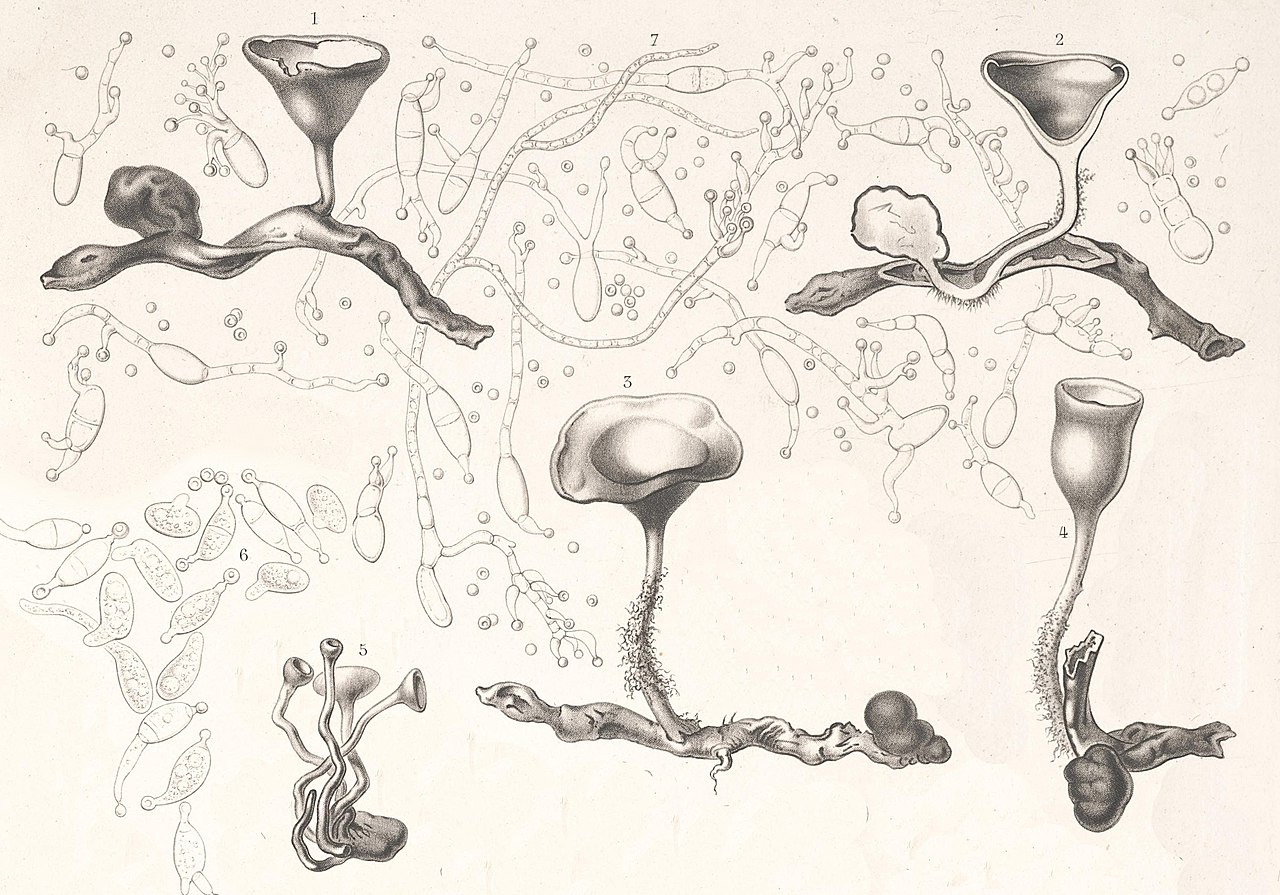
\includegraphics[width=\linewidth]{Figures/PezizaTuberosa.jpg}
%     \caption[Illustration of the fungus Dumontinia tuberosa.]{Illustration of the fungus Dumontinia tuberosa by physician, mycologist, and illustrator Charles Tulasne (1816–1884) in the book Selecta Fungorum Carpologia (1861–65). (Name of the original work: Peziza tuberosa parasite on Anemone nemorosa).}
%     \label{fig:figure-01}
% \end{figure}


\enlargethispage{3\baselineskip}
\begin{figure}[!hb]
\renewcommand\thesubfigure{A.\arabic{subfigure}} % Local change starts here
    \centering
    \begin{subfigure}{0.32\textwidth}
        \centering
        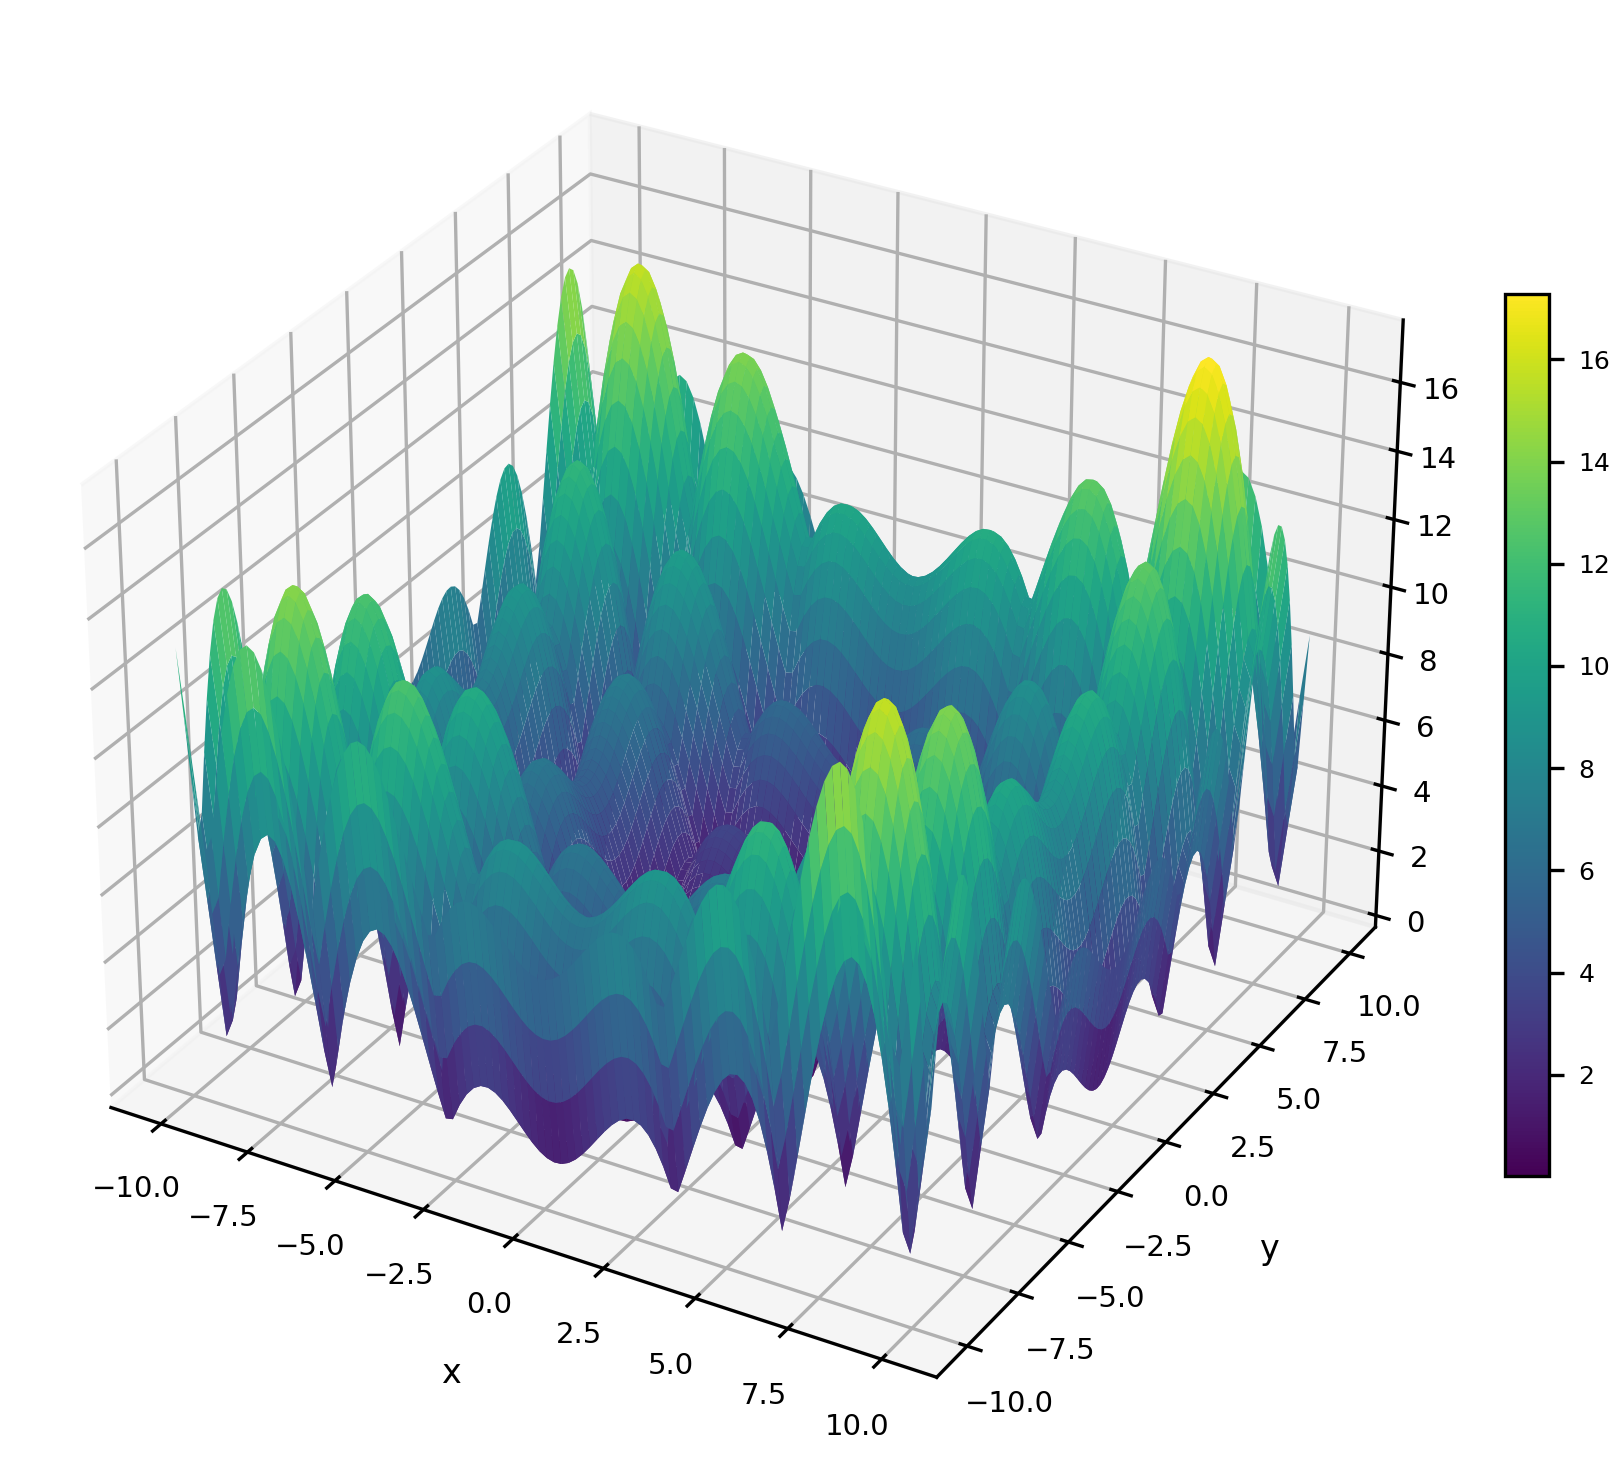
\includegraphics[width=1\textwidth]{Figures/benchmark_plots/Alpine_N1_maximized.png}
        \caption{Alpine N.1}
    \end{subfigure}
    % \hspace{.5cm} % Adjust the space as needed.
    \begin{subfigure}{0.32\textwidth}
        \centering
        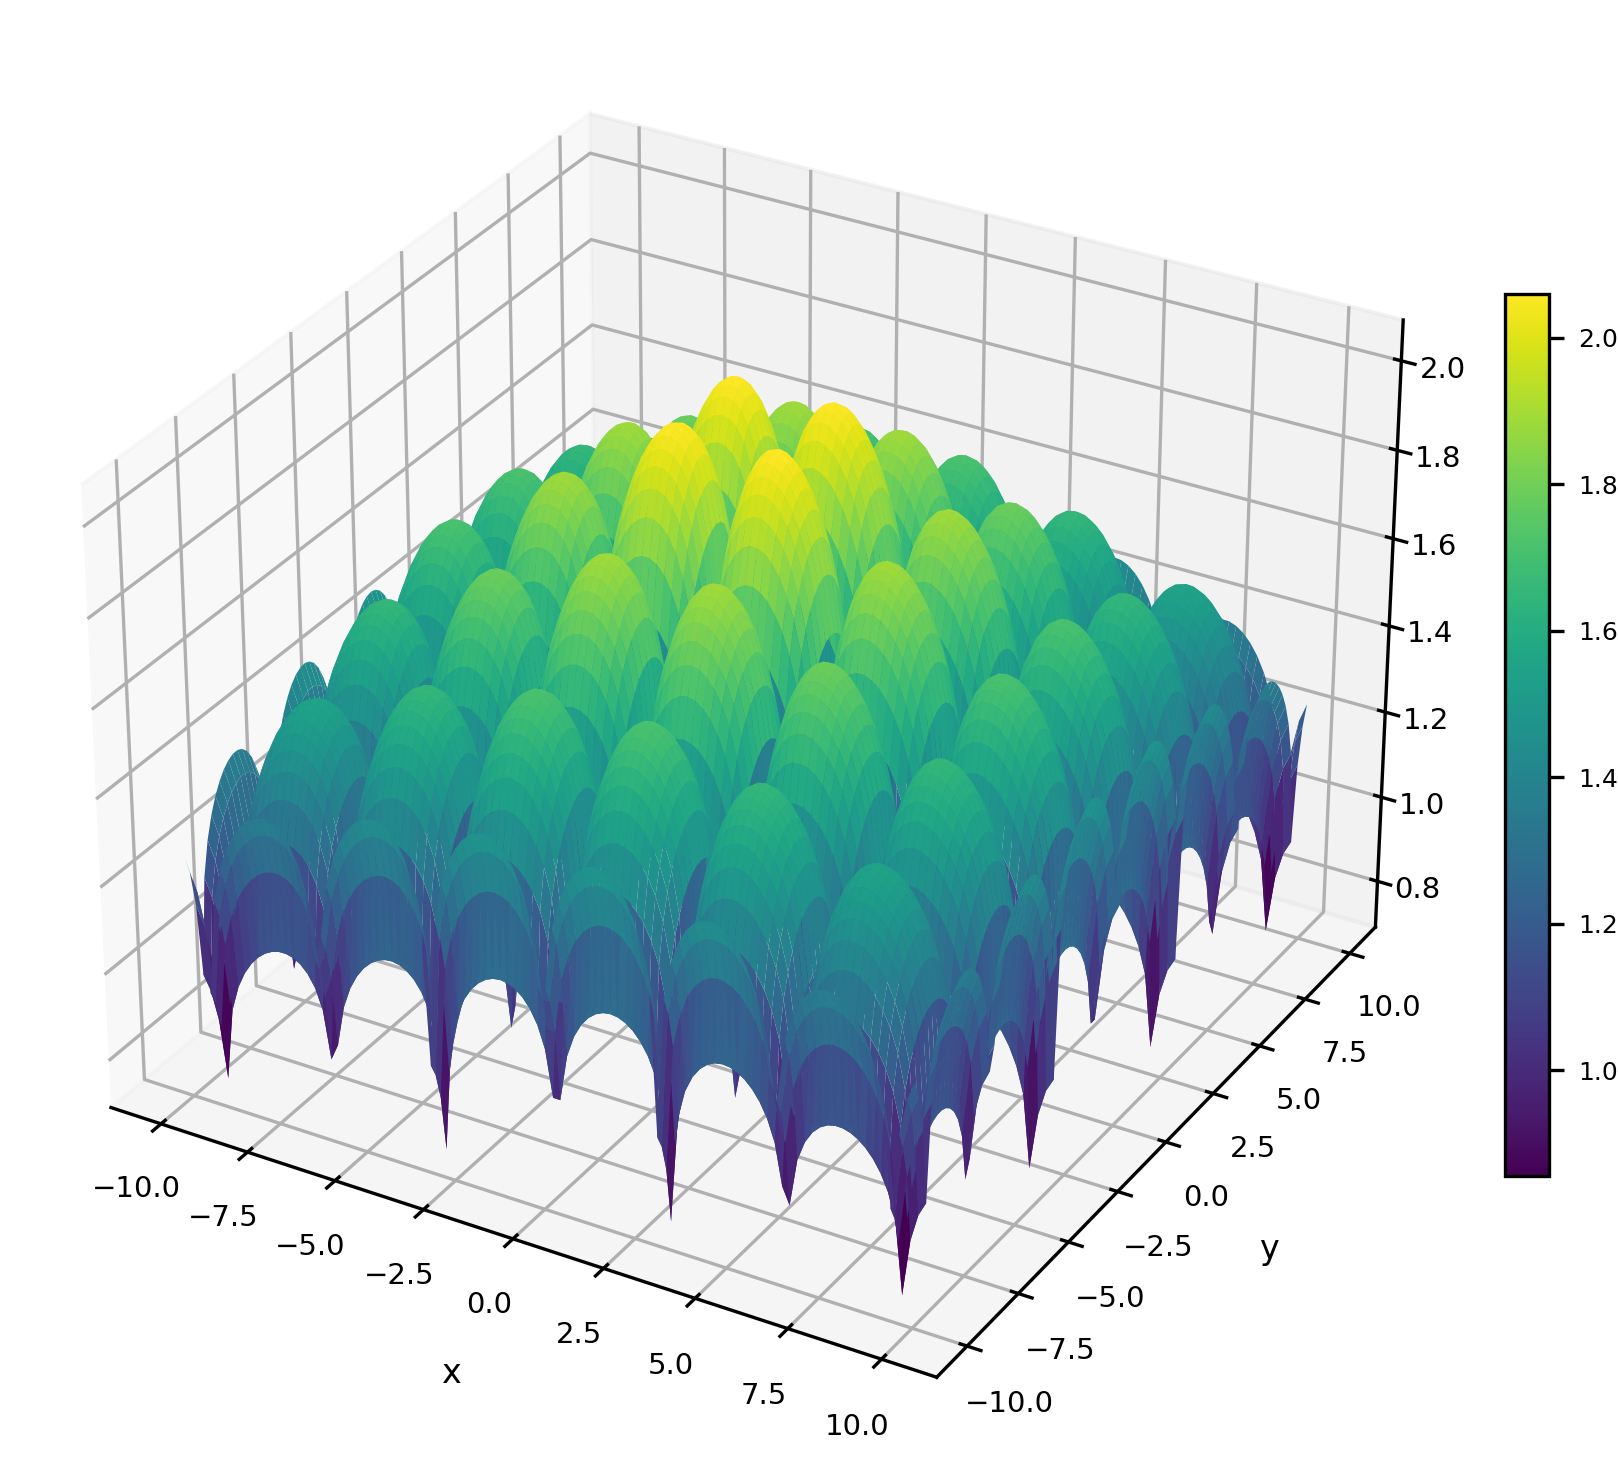
\includegraphics[width=1\textwidth]{Figures/benchmark_plots/Crowned_Cross_maximized.png}
        \caption{Crowned Cross}
    \end{subfigure}
    \begin{subfigure}{0.32\textwidth}
        \centering
        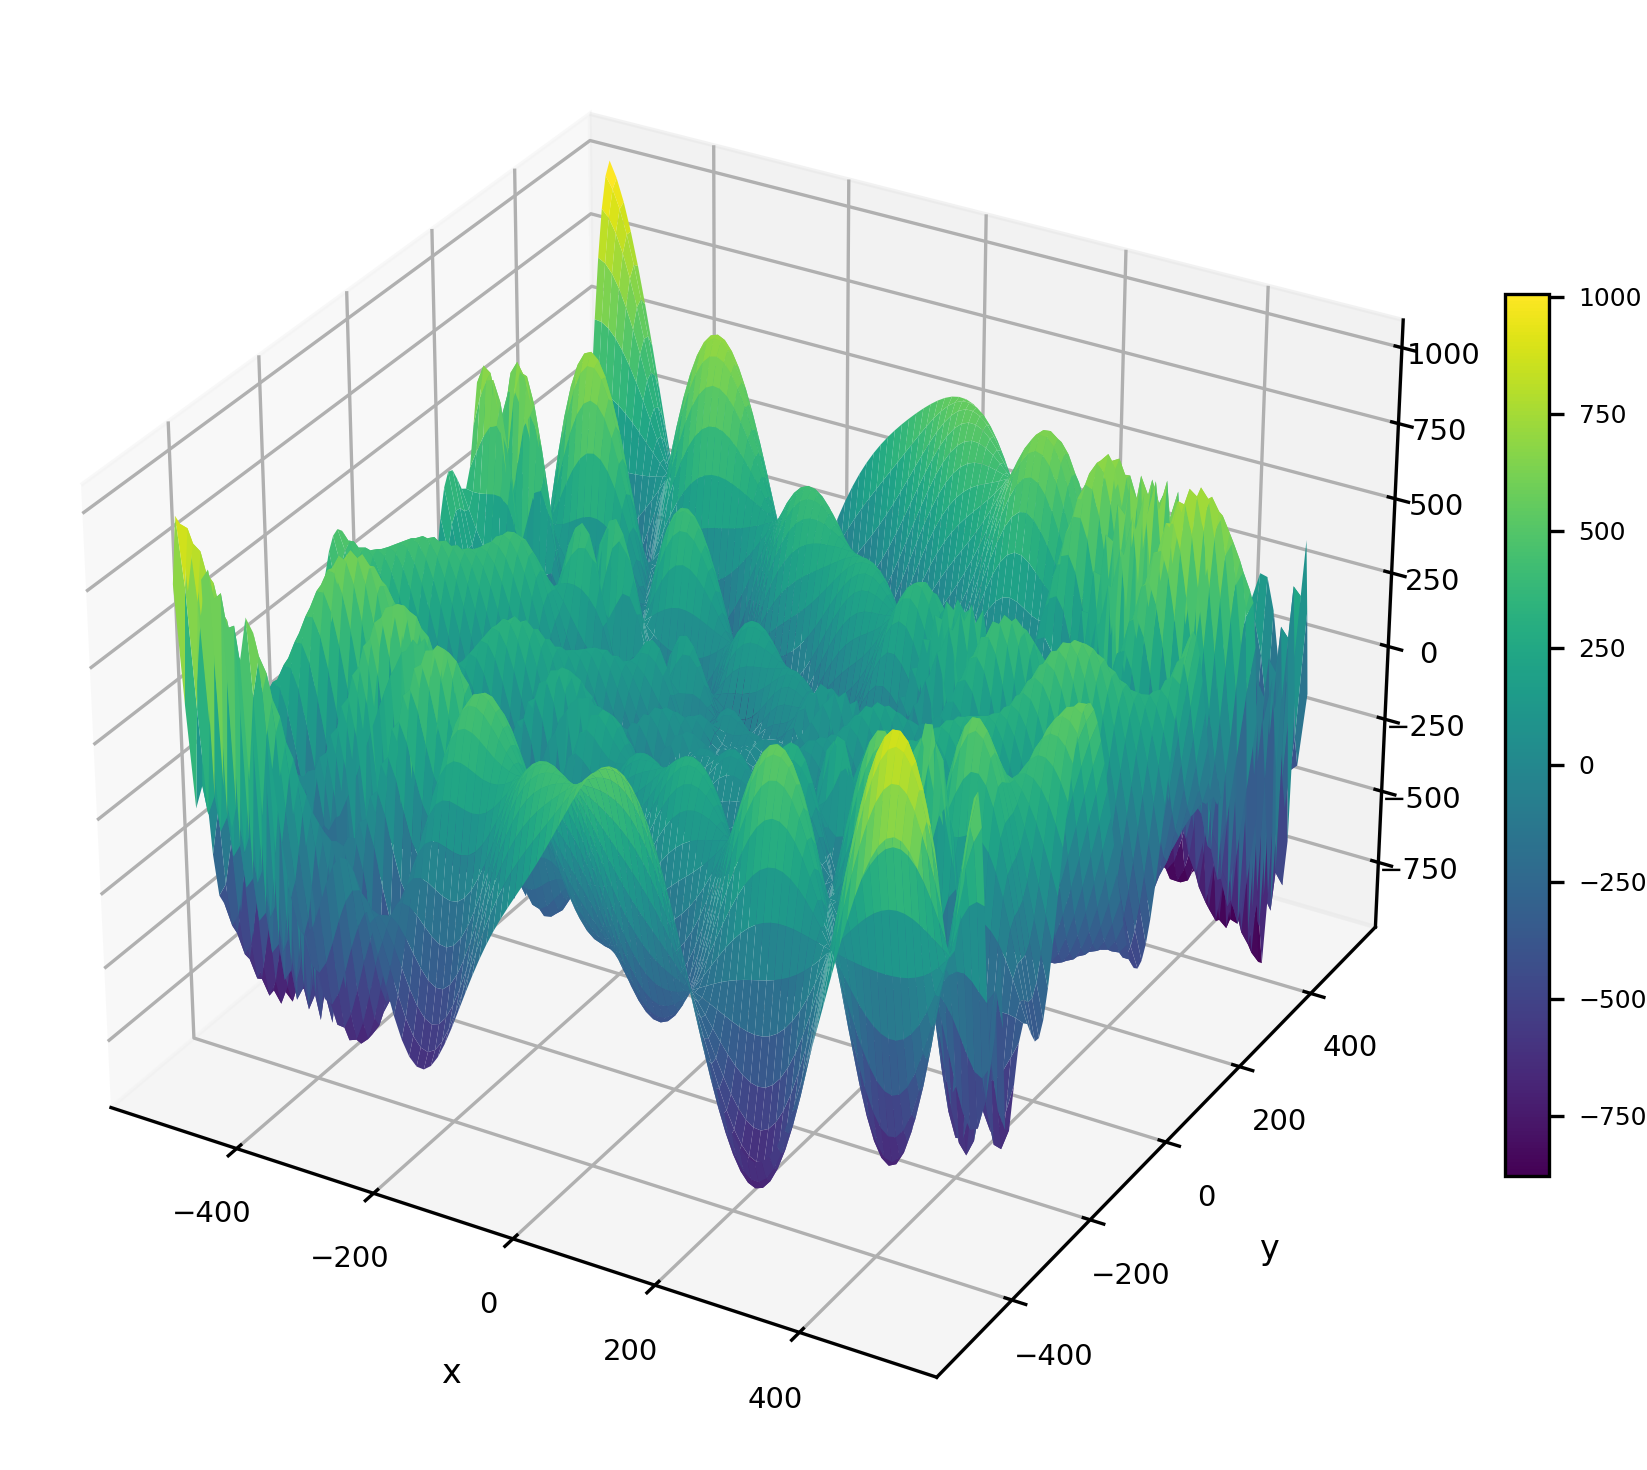
\includegraphics[width=1\textwidth]{Figures/benchmark_plots/Egg_Holder_maximized.png}
        \caption{Egg Holder}
    \end{subfigure}
    % \hspace{.5cm} % Adjust the space as needed.
    \begin{subfigure}{0.32\textwidth}
        \centering
        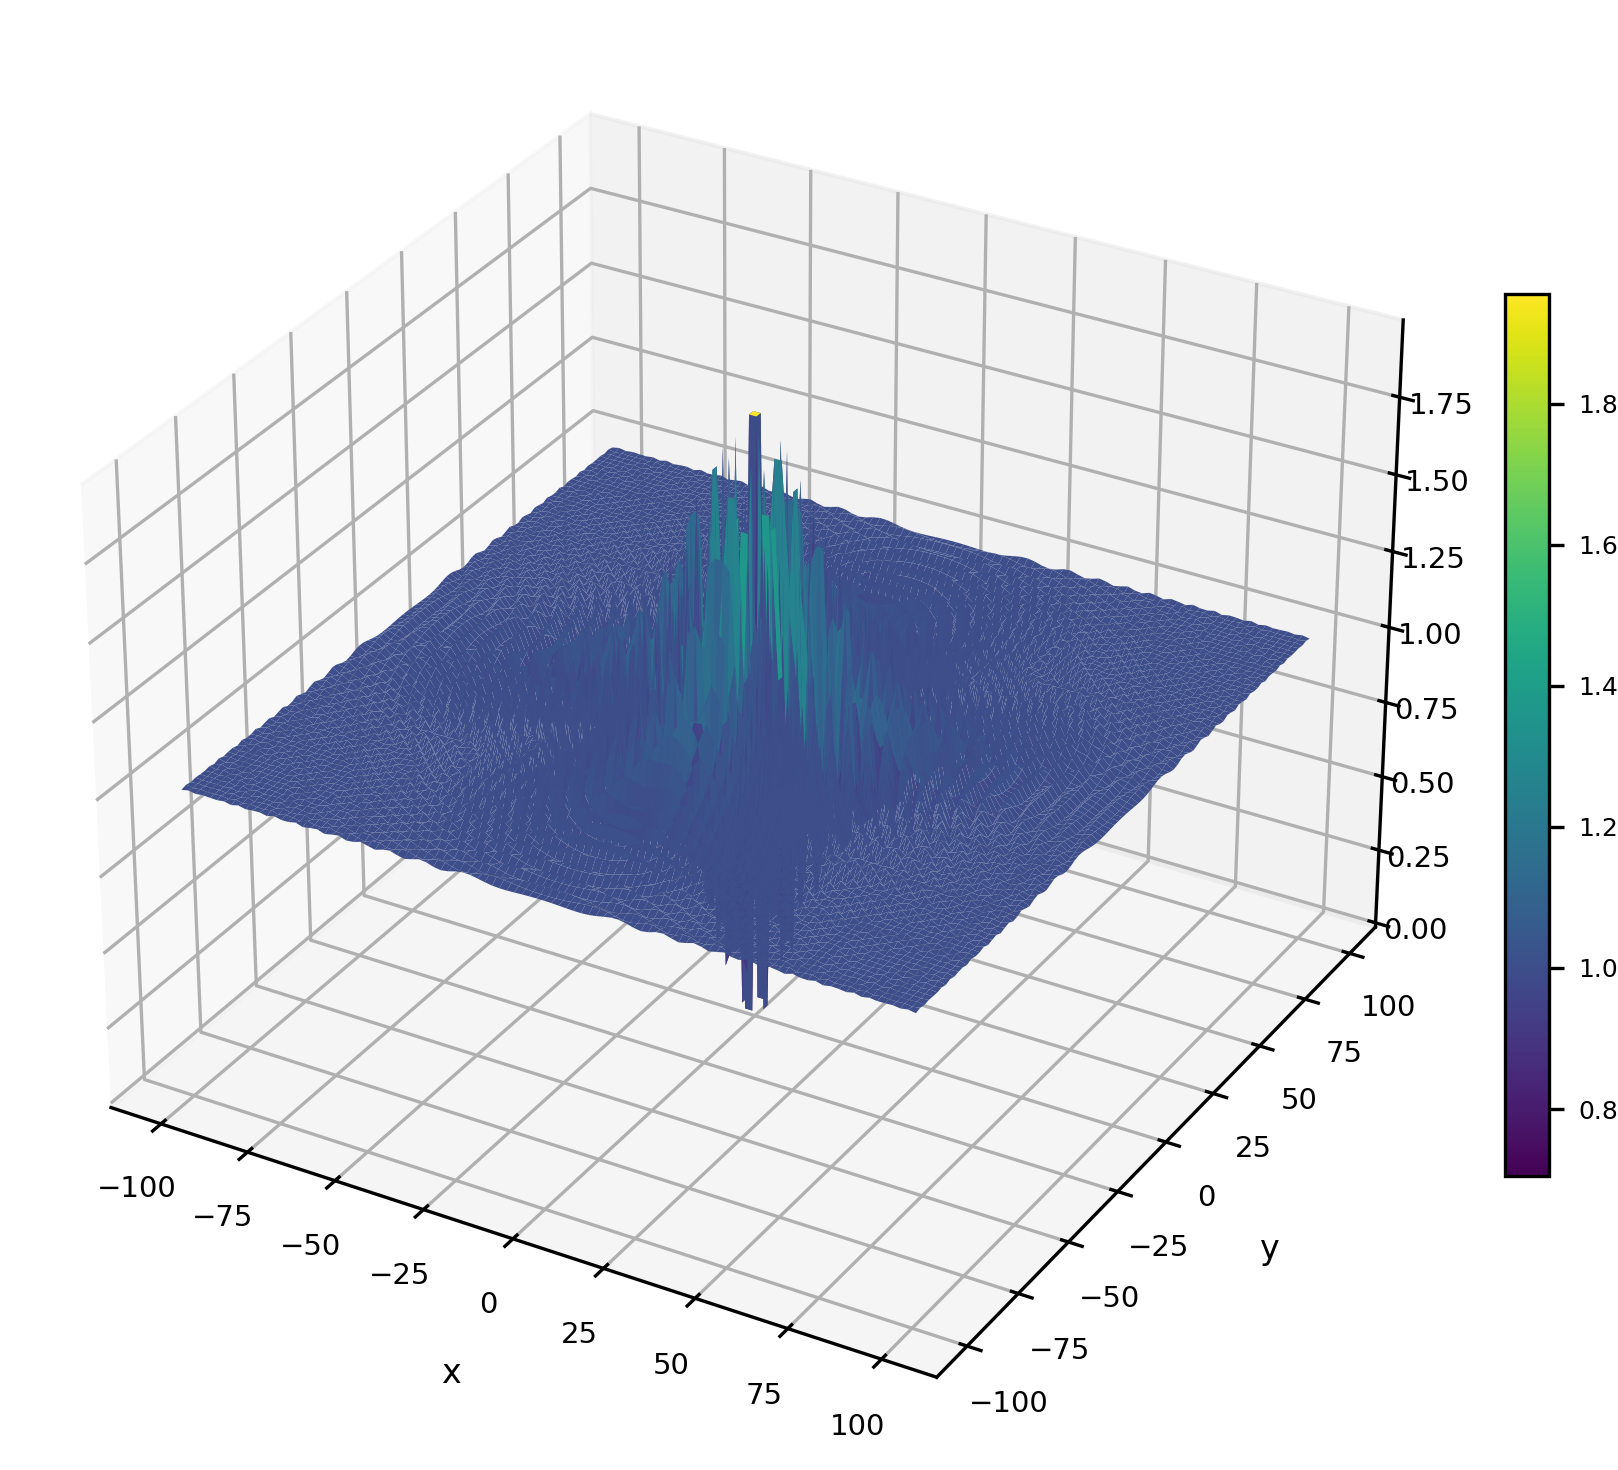
\includegraphics[width=1\textwidth]{Figures/benchmark_plots/Expanded_Shaffer_maximized.png}
        \caption{Expanded Shaffer (F6)}
    \end{subfigure}
        \begin{subfigure}{0.32\textwidth}
        \centering
        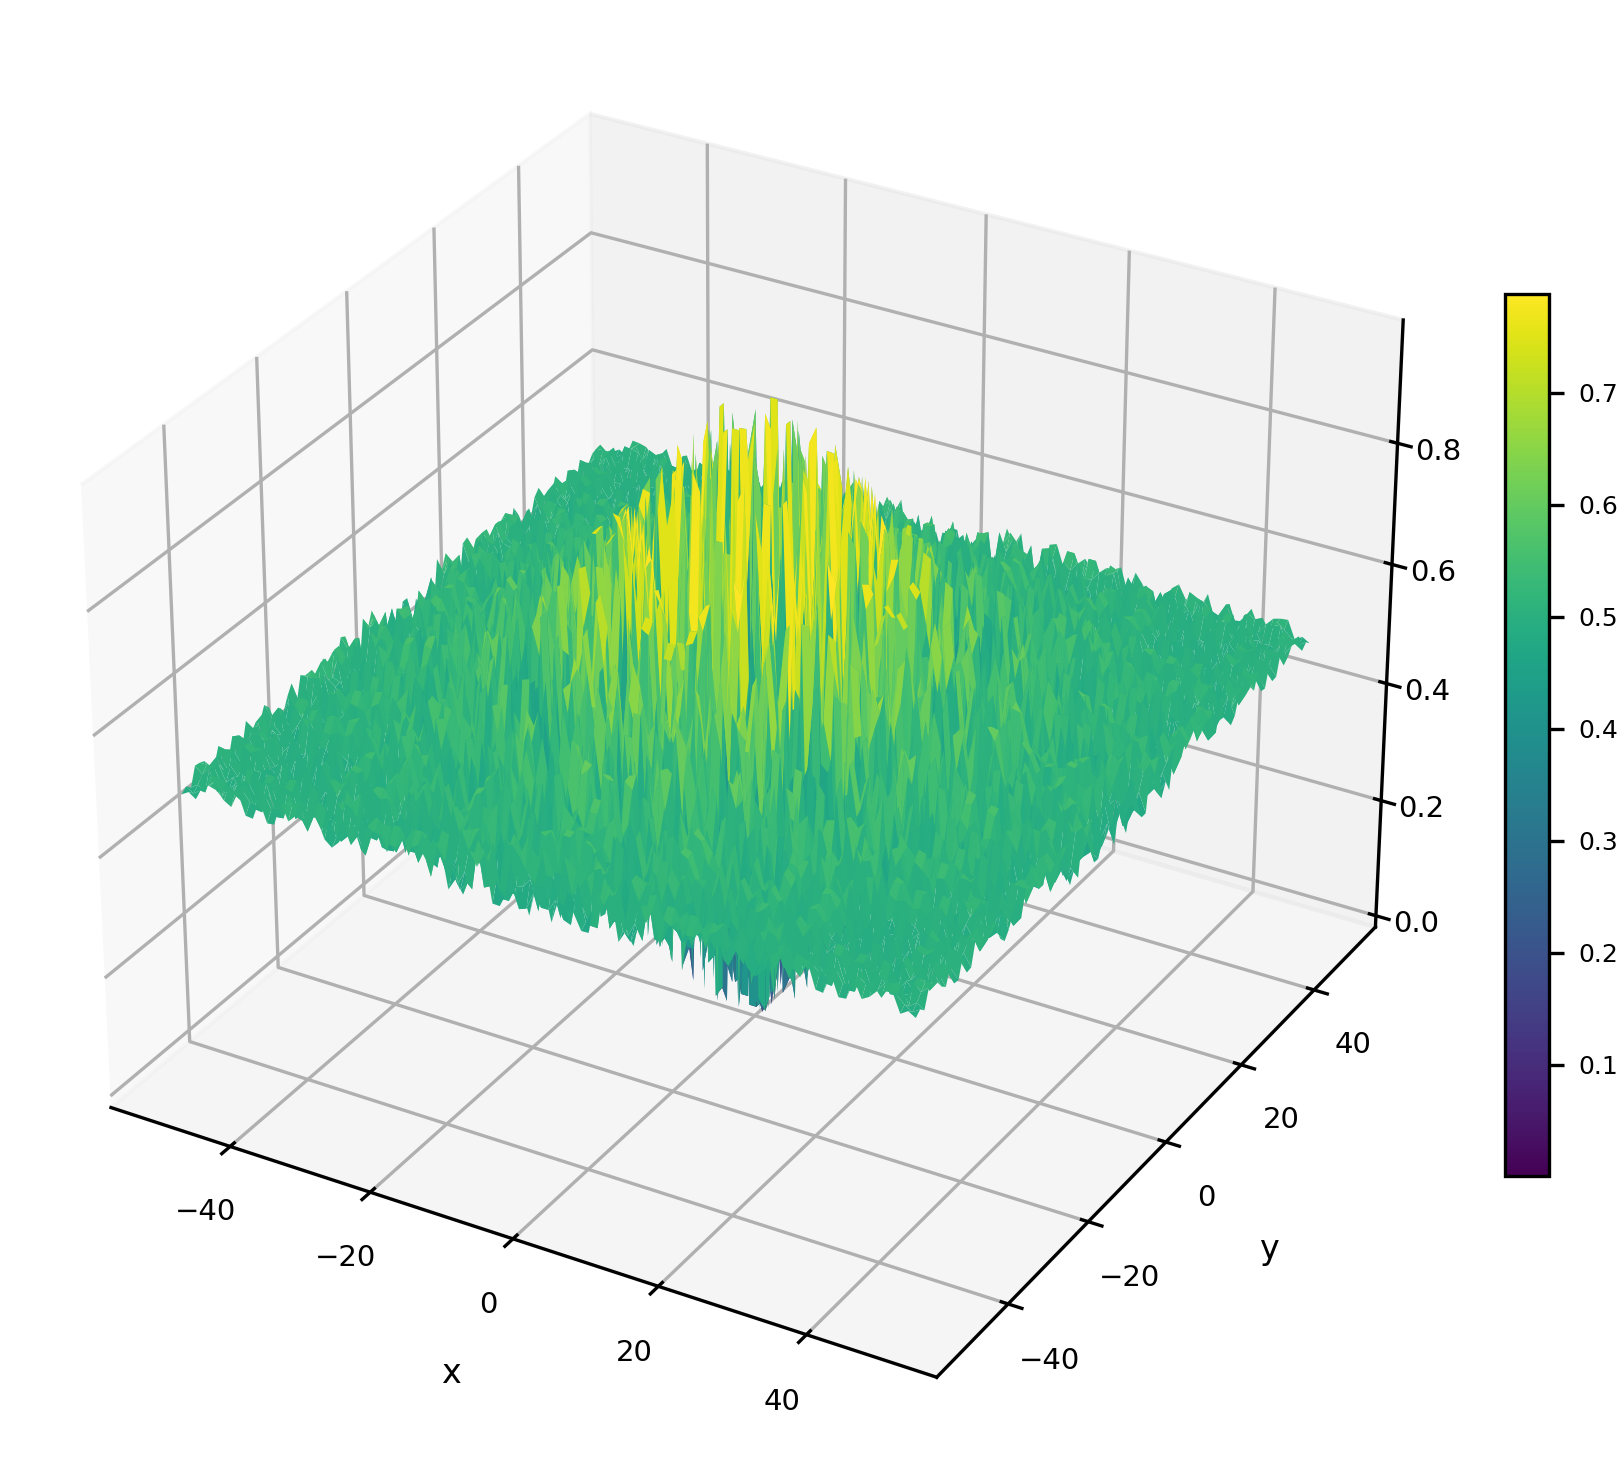
\includegraphics[width=1\textwidth]{Figures/benchmark_plots/Generalized_Schaffer_N1_maximized.png}
        \caption{Generalized Schaffer N1}
    \end{subfigure}
        \begin{subfigure}{0.32\textwidth}
        \centering
        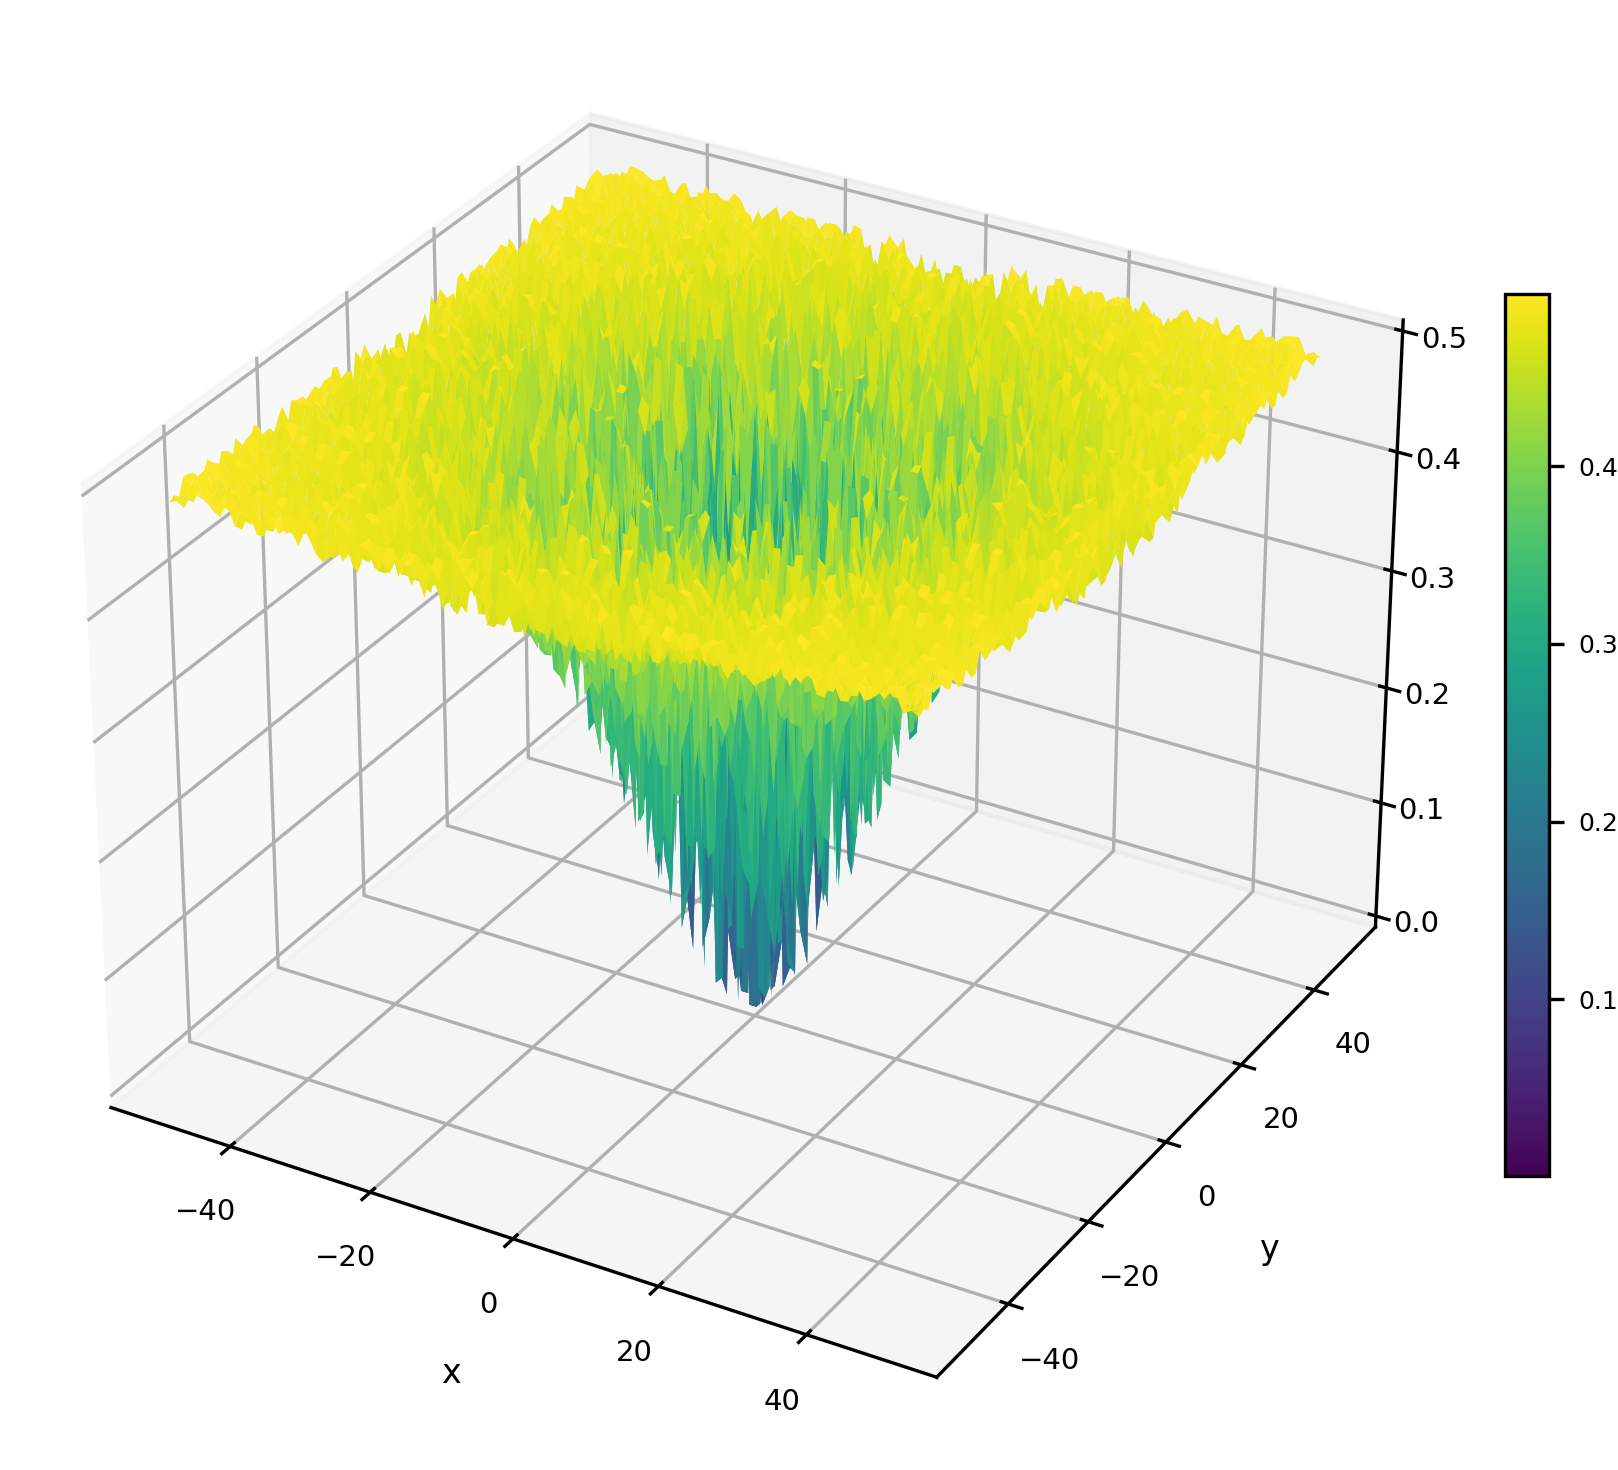
\includegraphics[width=1\textwidth]{Figures/benchmark_plots/Generalized_Schaffer_N2_maximized.png}
        \caption{Generalized Schaffer N2}
    \end{subfigure}
        \begin{subfigure}{0.32\textwidth}
        \centering
        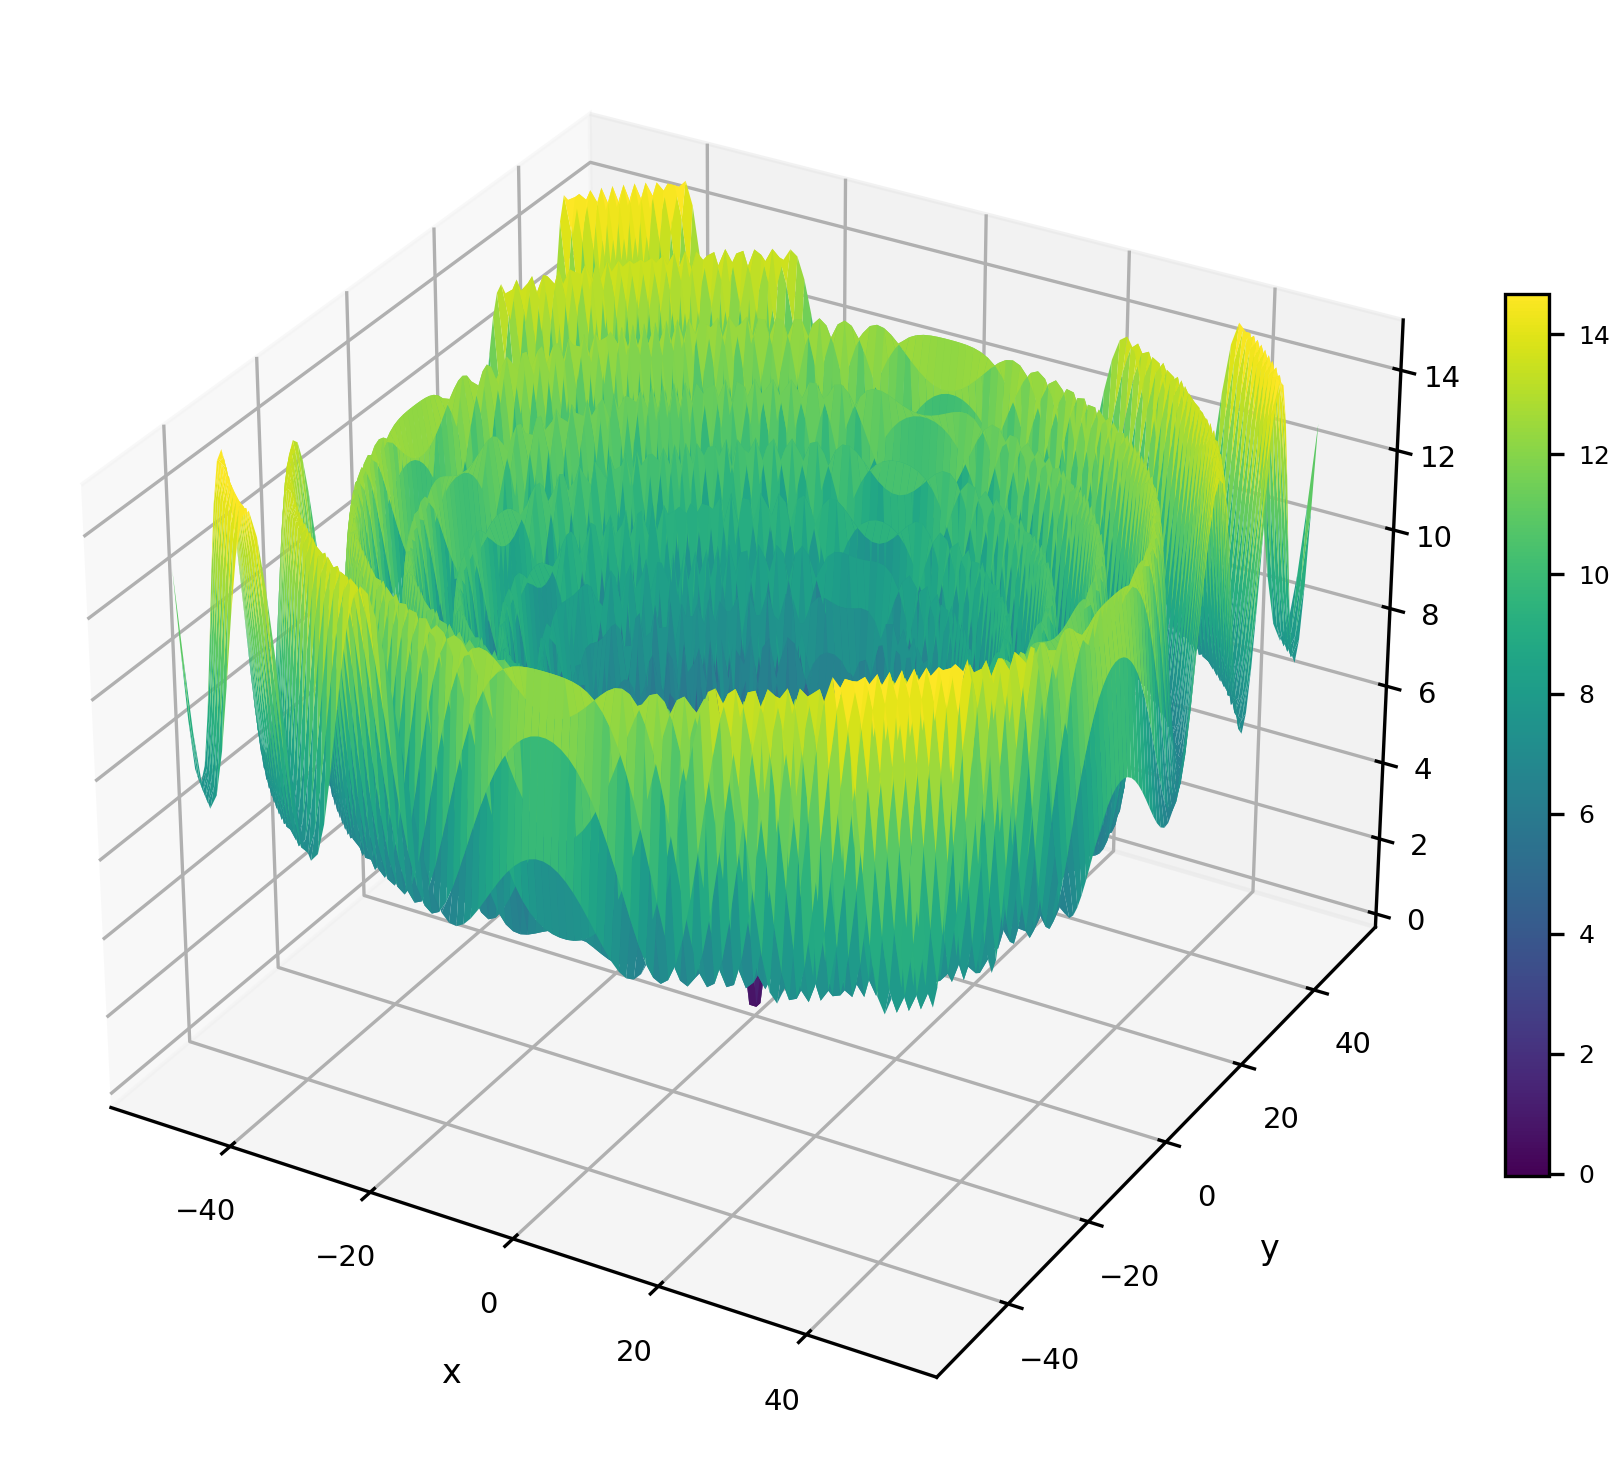
\includegraphics[width=1\textwidth]{Figures/benchmark_plots/Generalized_Schaffer_N3_maximized.png}
        \caption{Generalized Schaffer N3}
    \end{subfigure}
      \begin{subfigure}{0.32\textwidth}
        \centering
        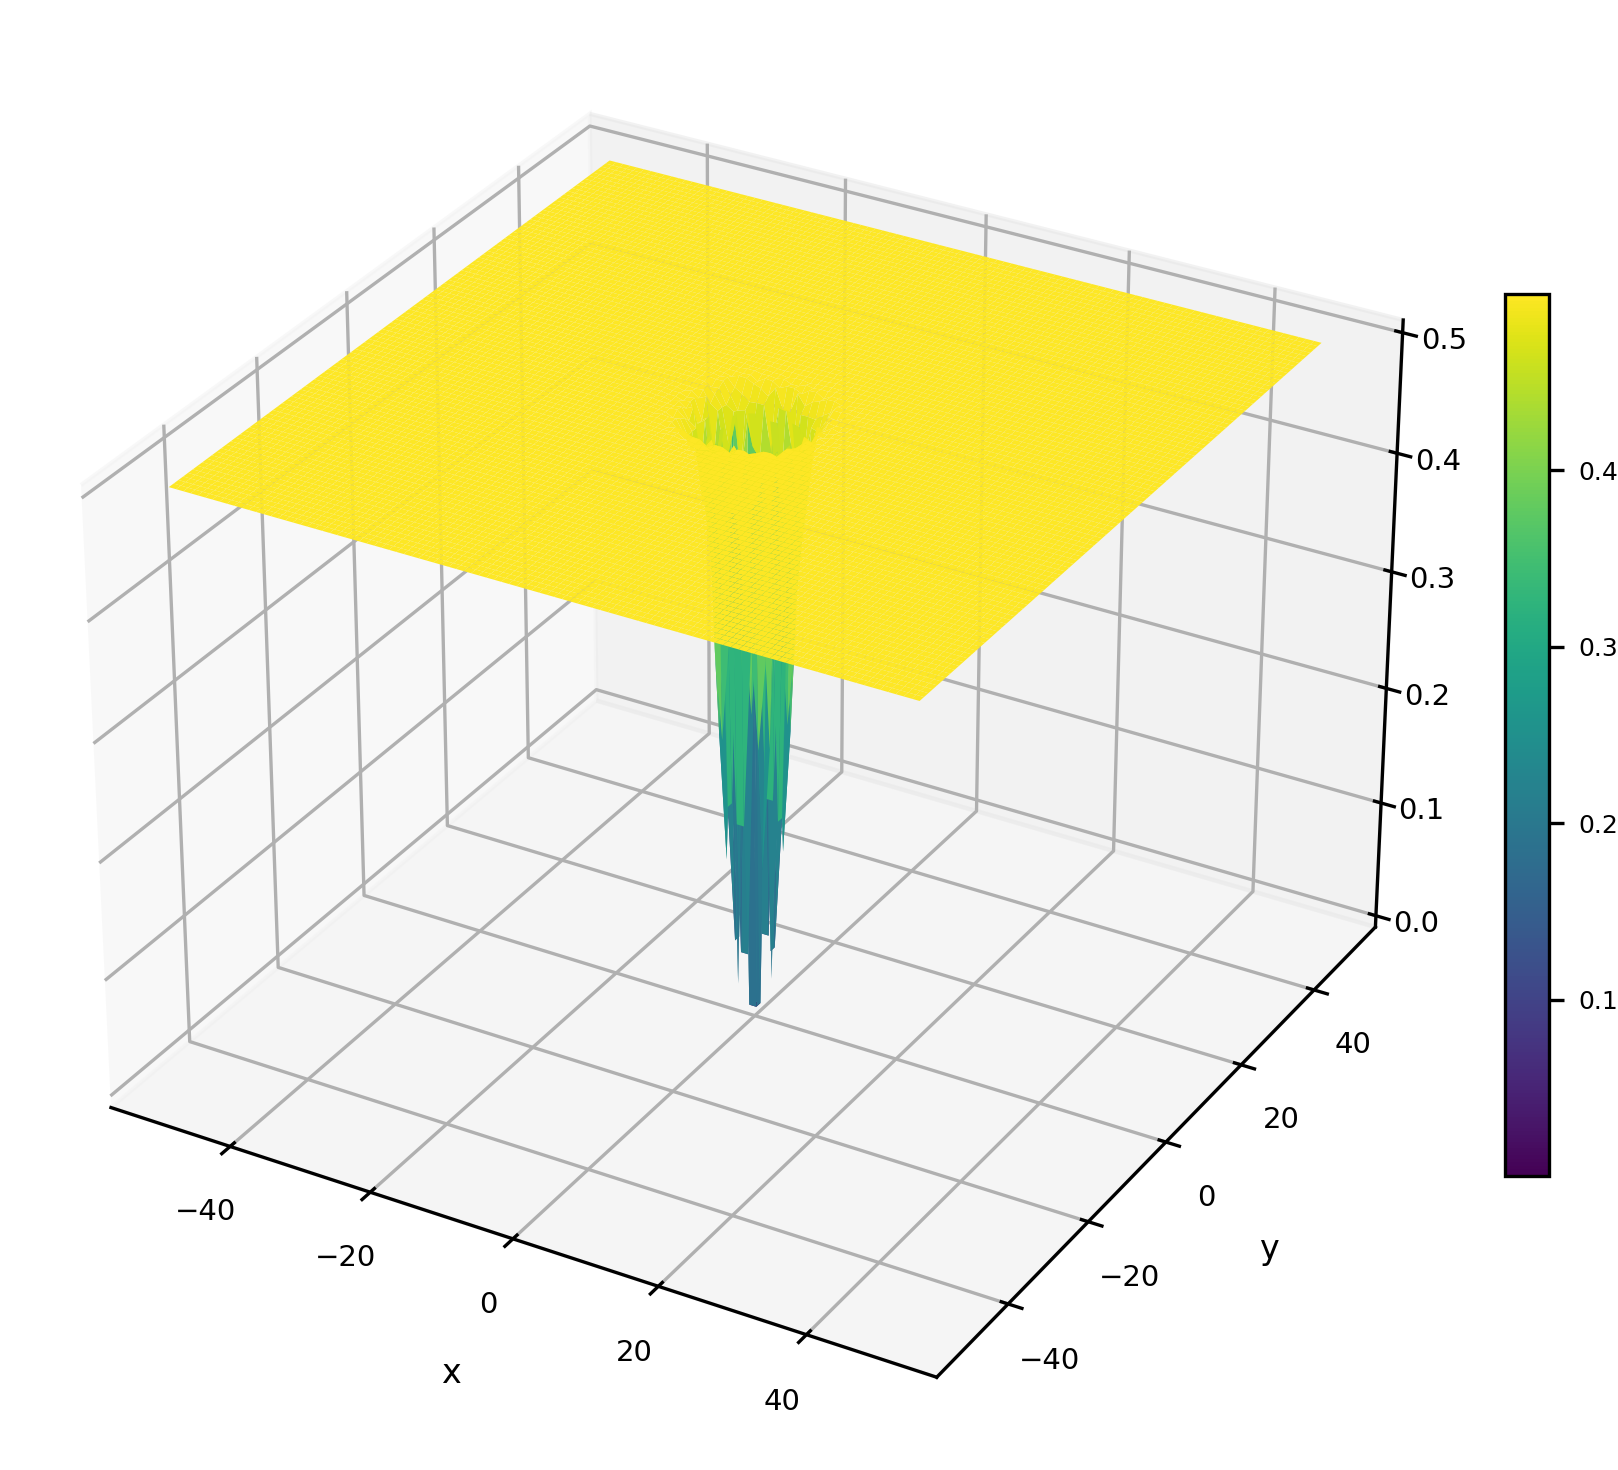
\includegraphics[width=1\textwidth]{Figures/benchmark_plots/Generalized_Schaffer_N4_maximized.png}
        \caption{Generalized Schaffer N4}
    \end{subfigure}
        \begin{subfigure}{0.32\textwidth}
        \centering
        \includegraphics[width=1\textwidth]{Figures/benchmark_plots/Generalized_Schmidt–Vetters_maximized.png}
        \caption{Schmidt–Vetters}
    \end{subfigure}
    \caption[Visualizations of benchmark problem landscapes]{Two-dimensional visualizations of benchmark problem landscapes.}
\end{figure}


\begin{figure}[p]\ContinuedFloat
\renewcommand\thesubfigure{A.\arabic{subfigure}} % Local change starts here
    \centering
    \begin{subfigure}{0.32\textwidth}
        \centering
        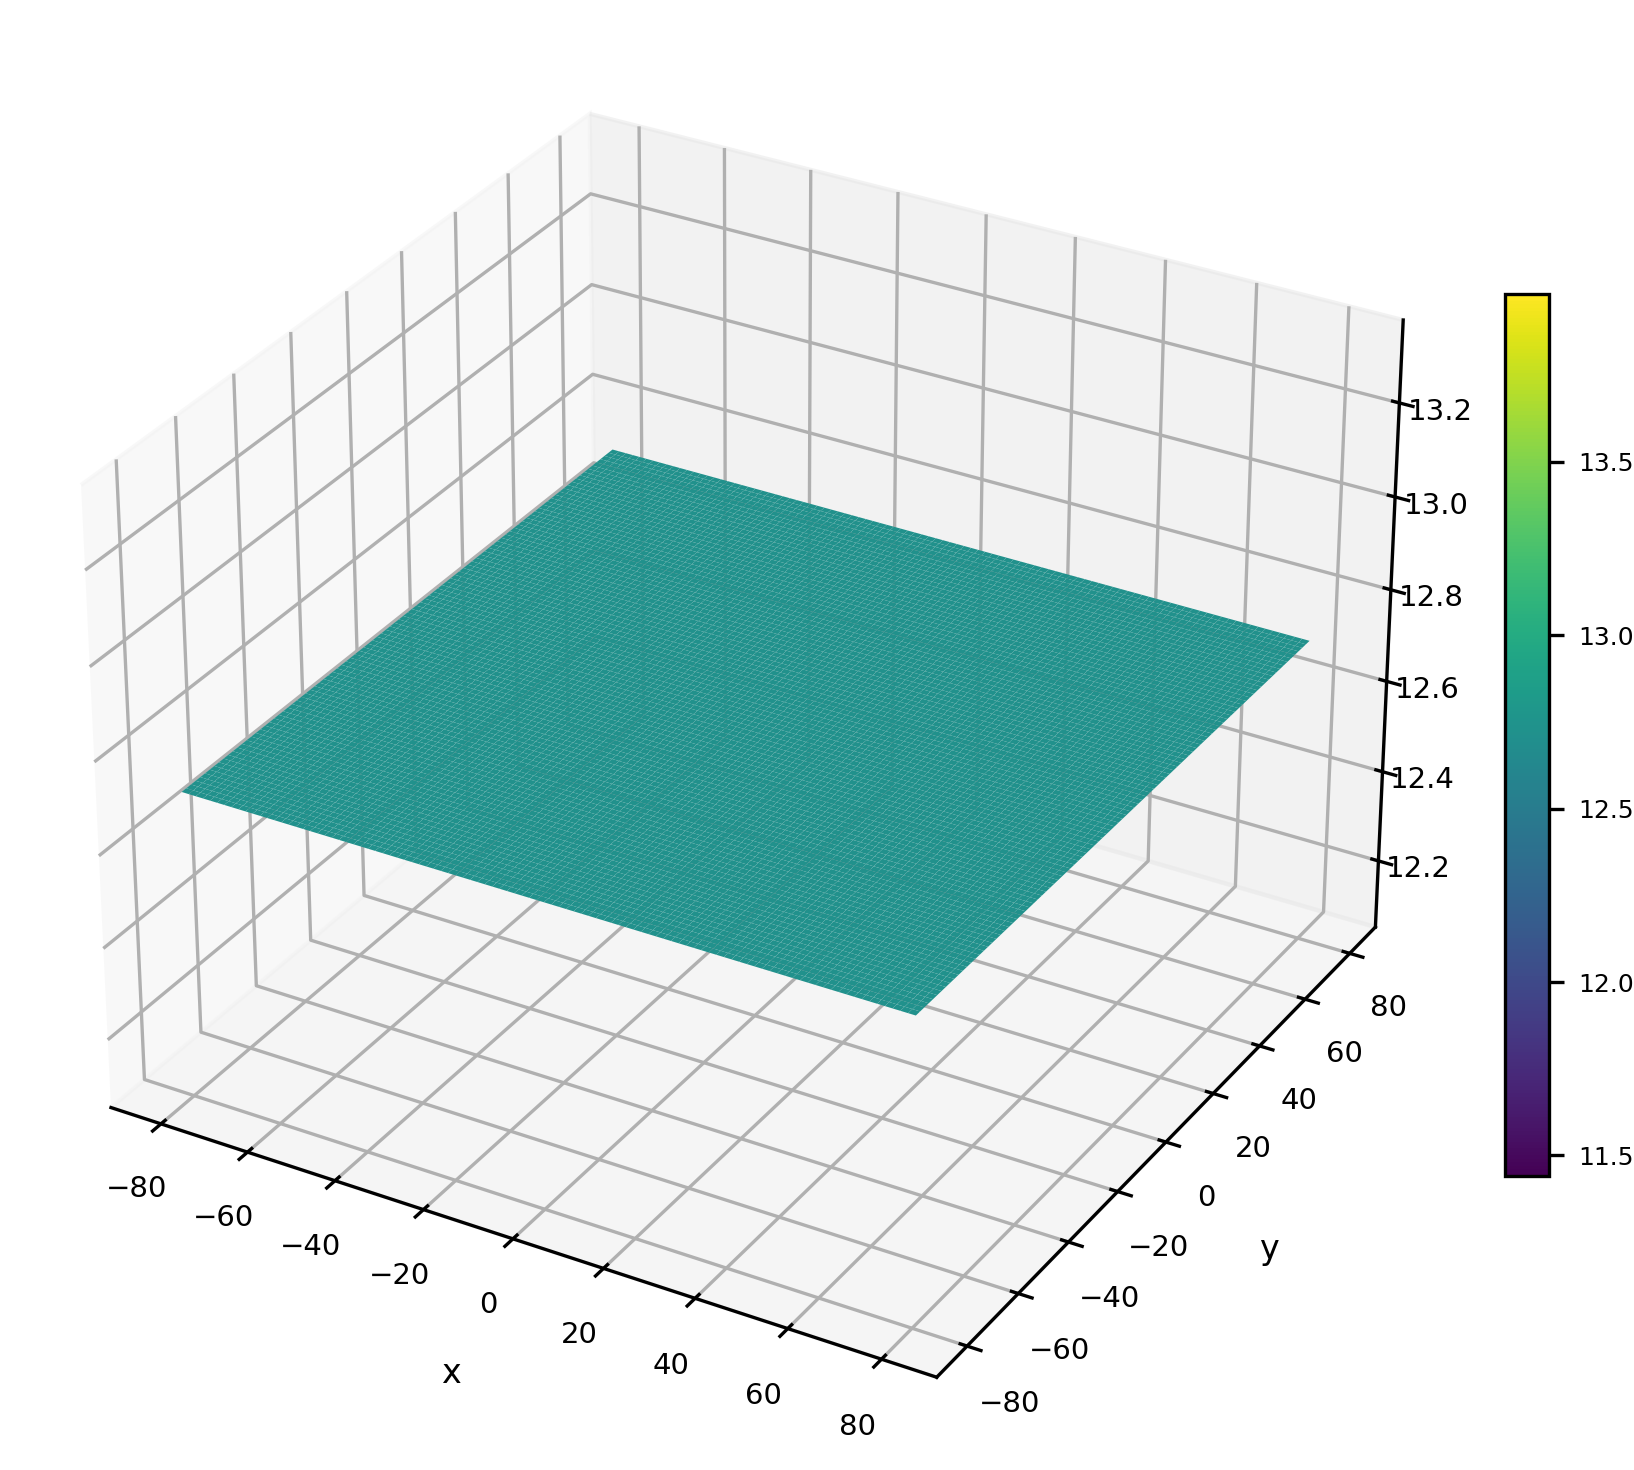
\includegraphics[width=1\textwidth]{Figures/benchmark_plots/Lennard_Jones_Minimum_Energy_Cluster_maximized.png}
        \caption{Lennard‑Jones}
    \end{subfigure}
    \begin{subfigure}{0.32\textwidth}
        \centering
        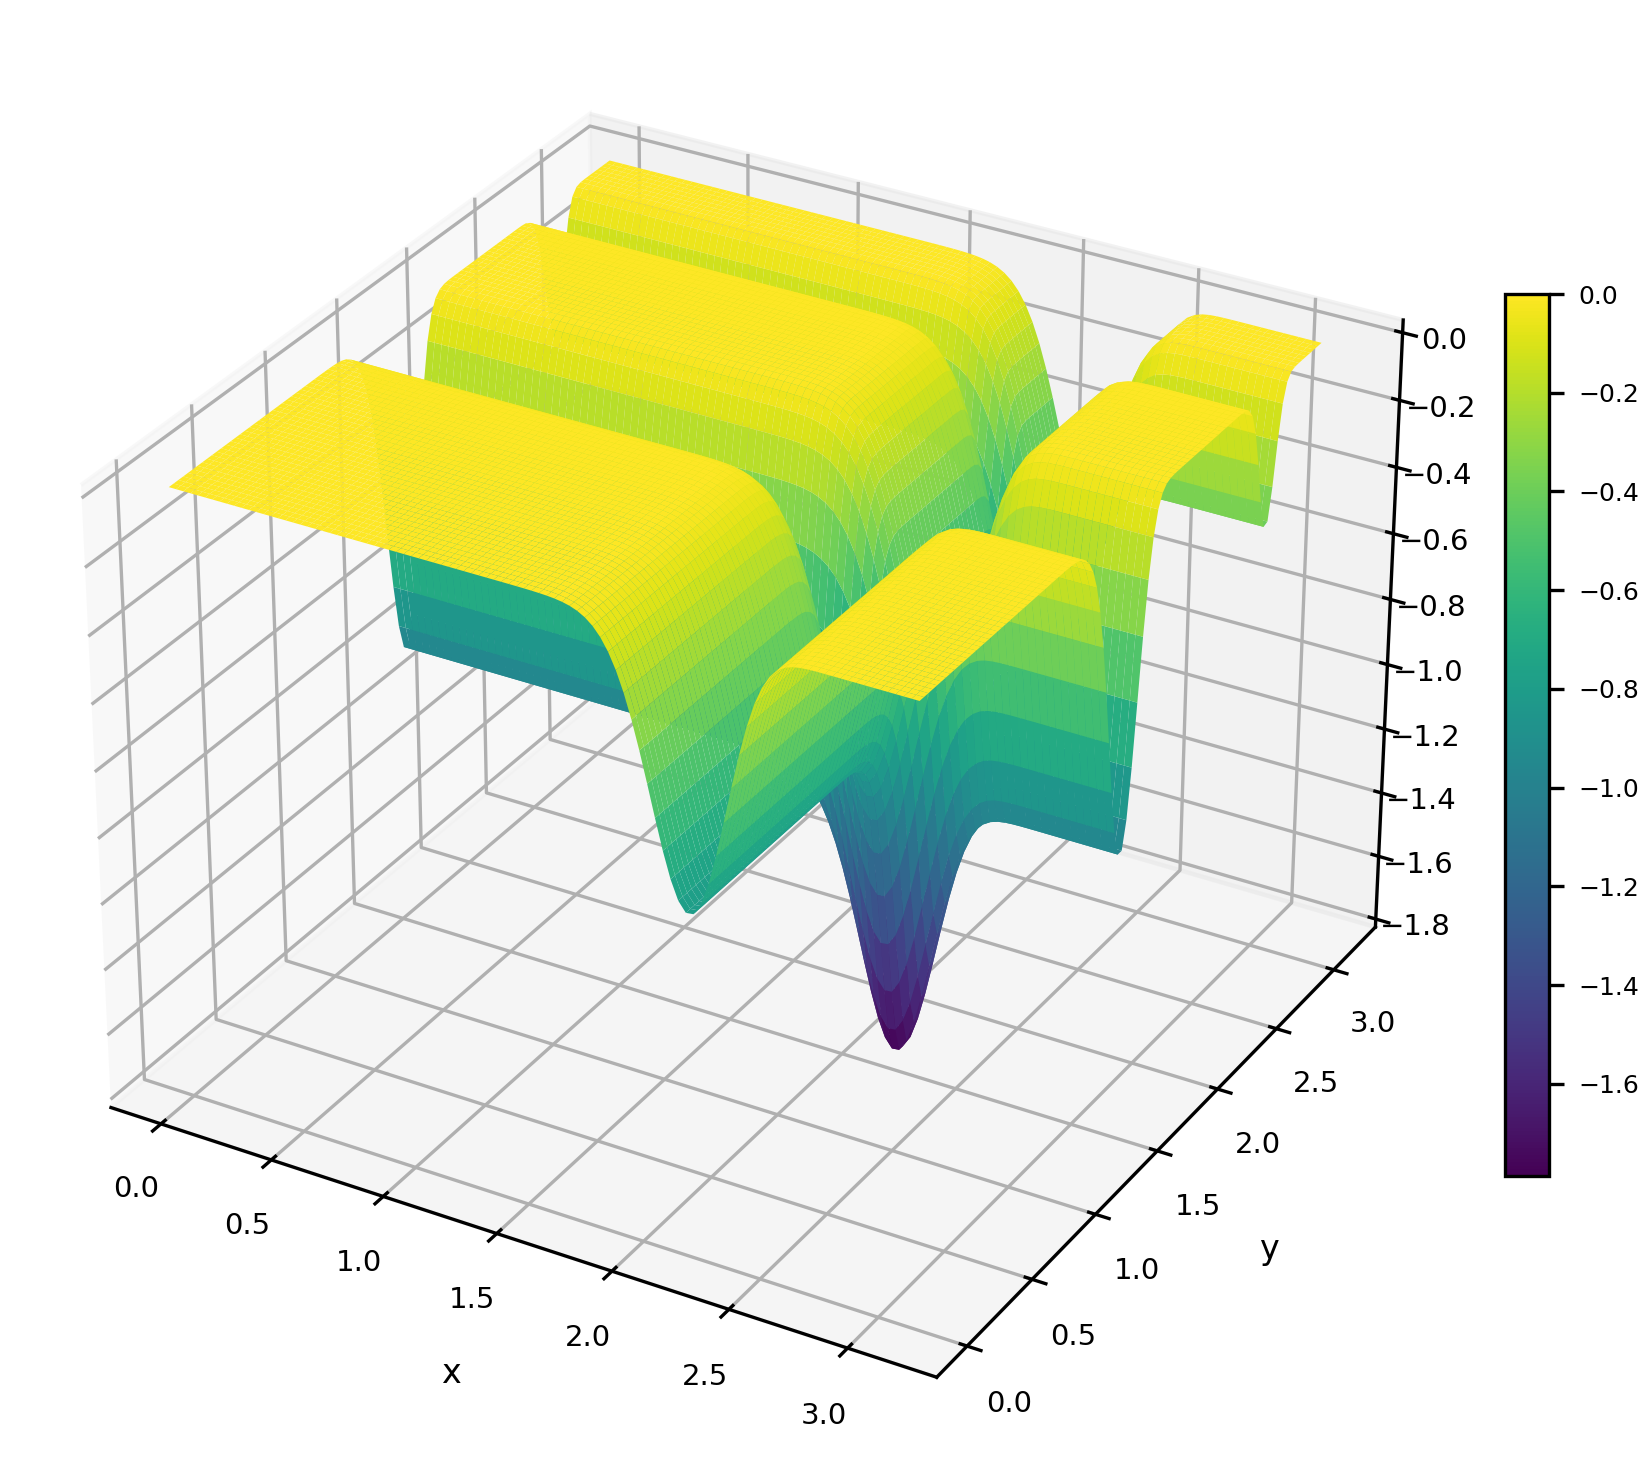
\includegraphics[width=1\textwidth]{Figures/benchmark_plots/Michalewicz_maximized.png}
        \caption{Michalewicz}
    \end{subfigure}
    % \hspace{.5cm} % Adjust the space as needed.
    \begin{subfigure}{0.32\textwidth}
        \centering
        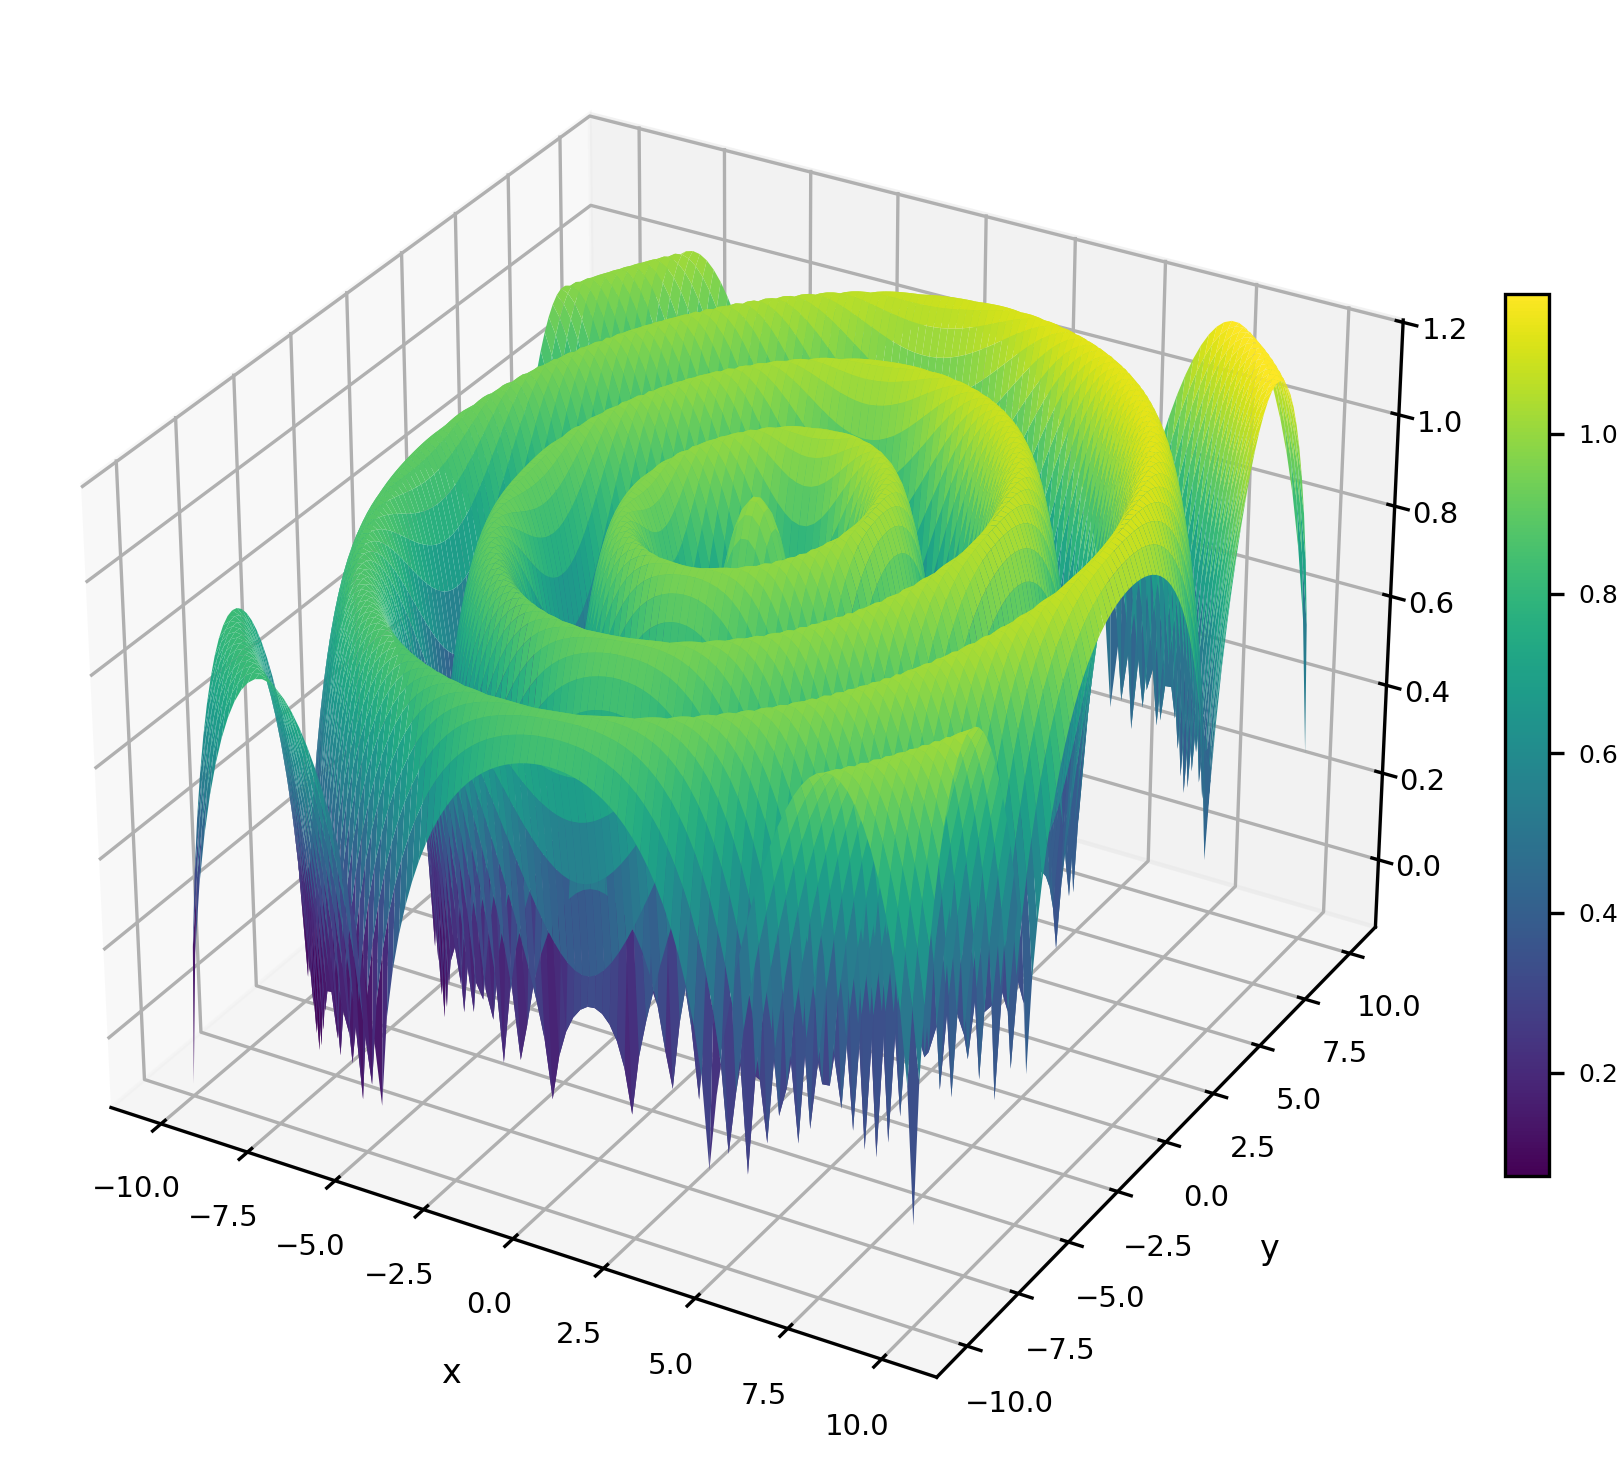
\includegraphics[width=1\textwidth]{Figures/benchmark_plots/Mishra_N3_maximized.png}
        \caption{Mishra 03}
    \end{subfigure}
    \begin{subfigure}{0.48\textwidth}
        \centering
        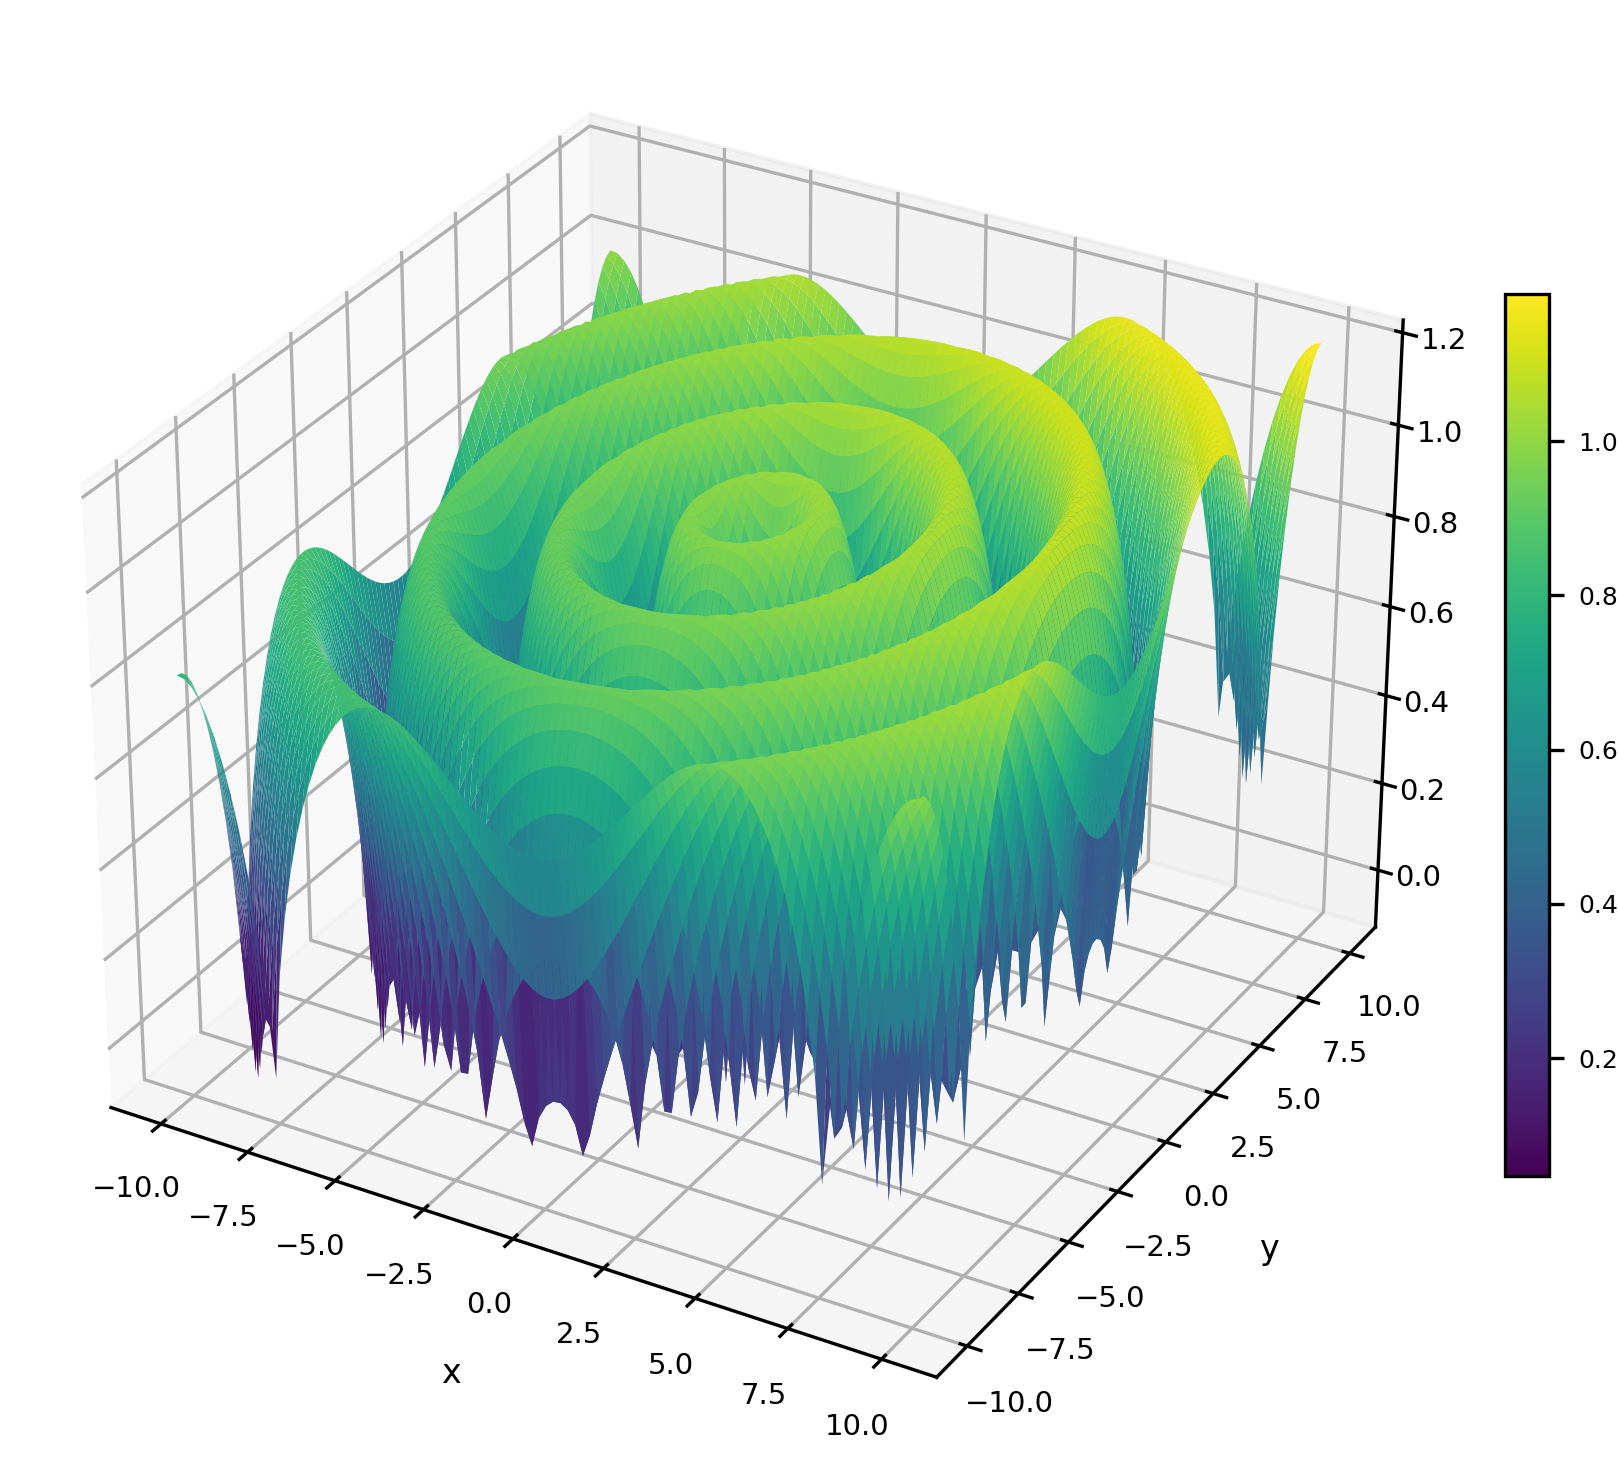
\includegraphics[width=1\textwidth]{Figures/benchmark_plots/Mishra_N4_maximized.png}
        \caption{Mishra 04}
    \end{subfigure}
    % \hspace{.5cm} % Adjust the space as needed.
    \begin{subfigure}{0.48\textwidth}
        \centering
        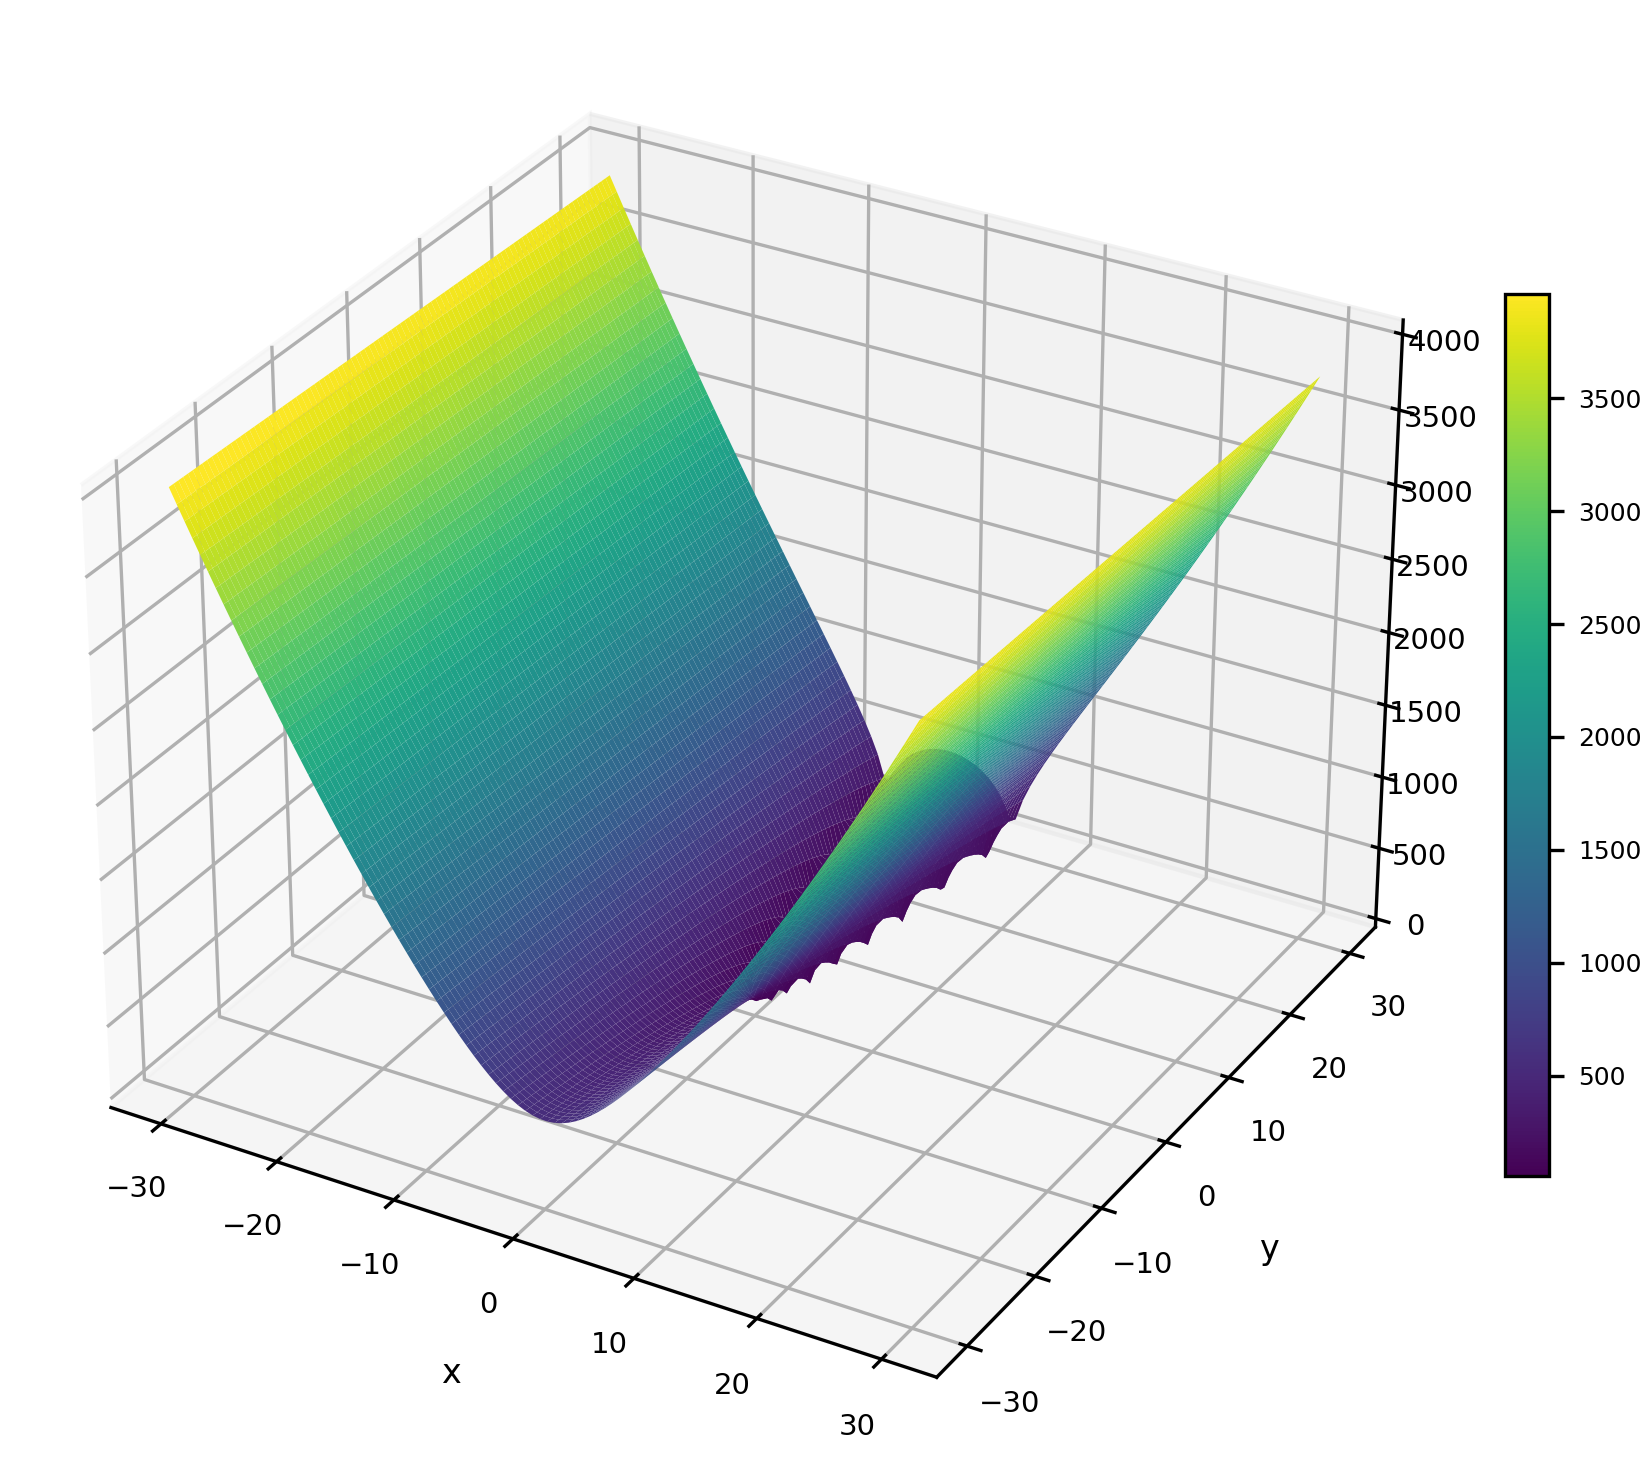
\includegraphics[width=1\textwidth]{Figures/benchmark_plots/Modified_Rosenbrock_No.02___Hollow_Ground_Bent_Knife_Edge_maximized.png}
        \caption{Modified Rosenbrock N.2}
    \end{subfigure}
    \begin{subfigure}{0.32\textwidth}
        \centering
        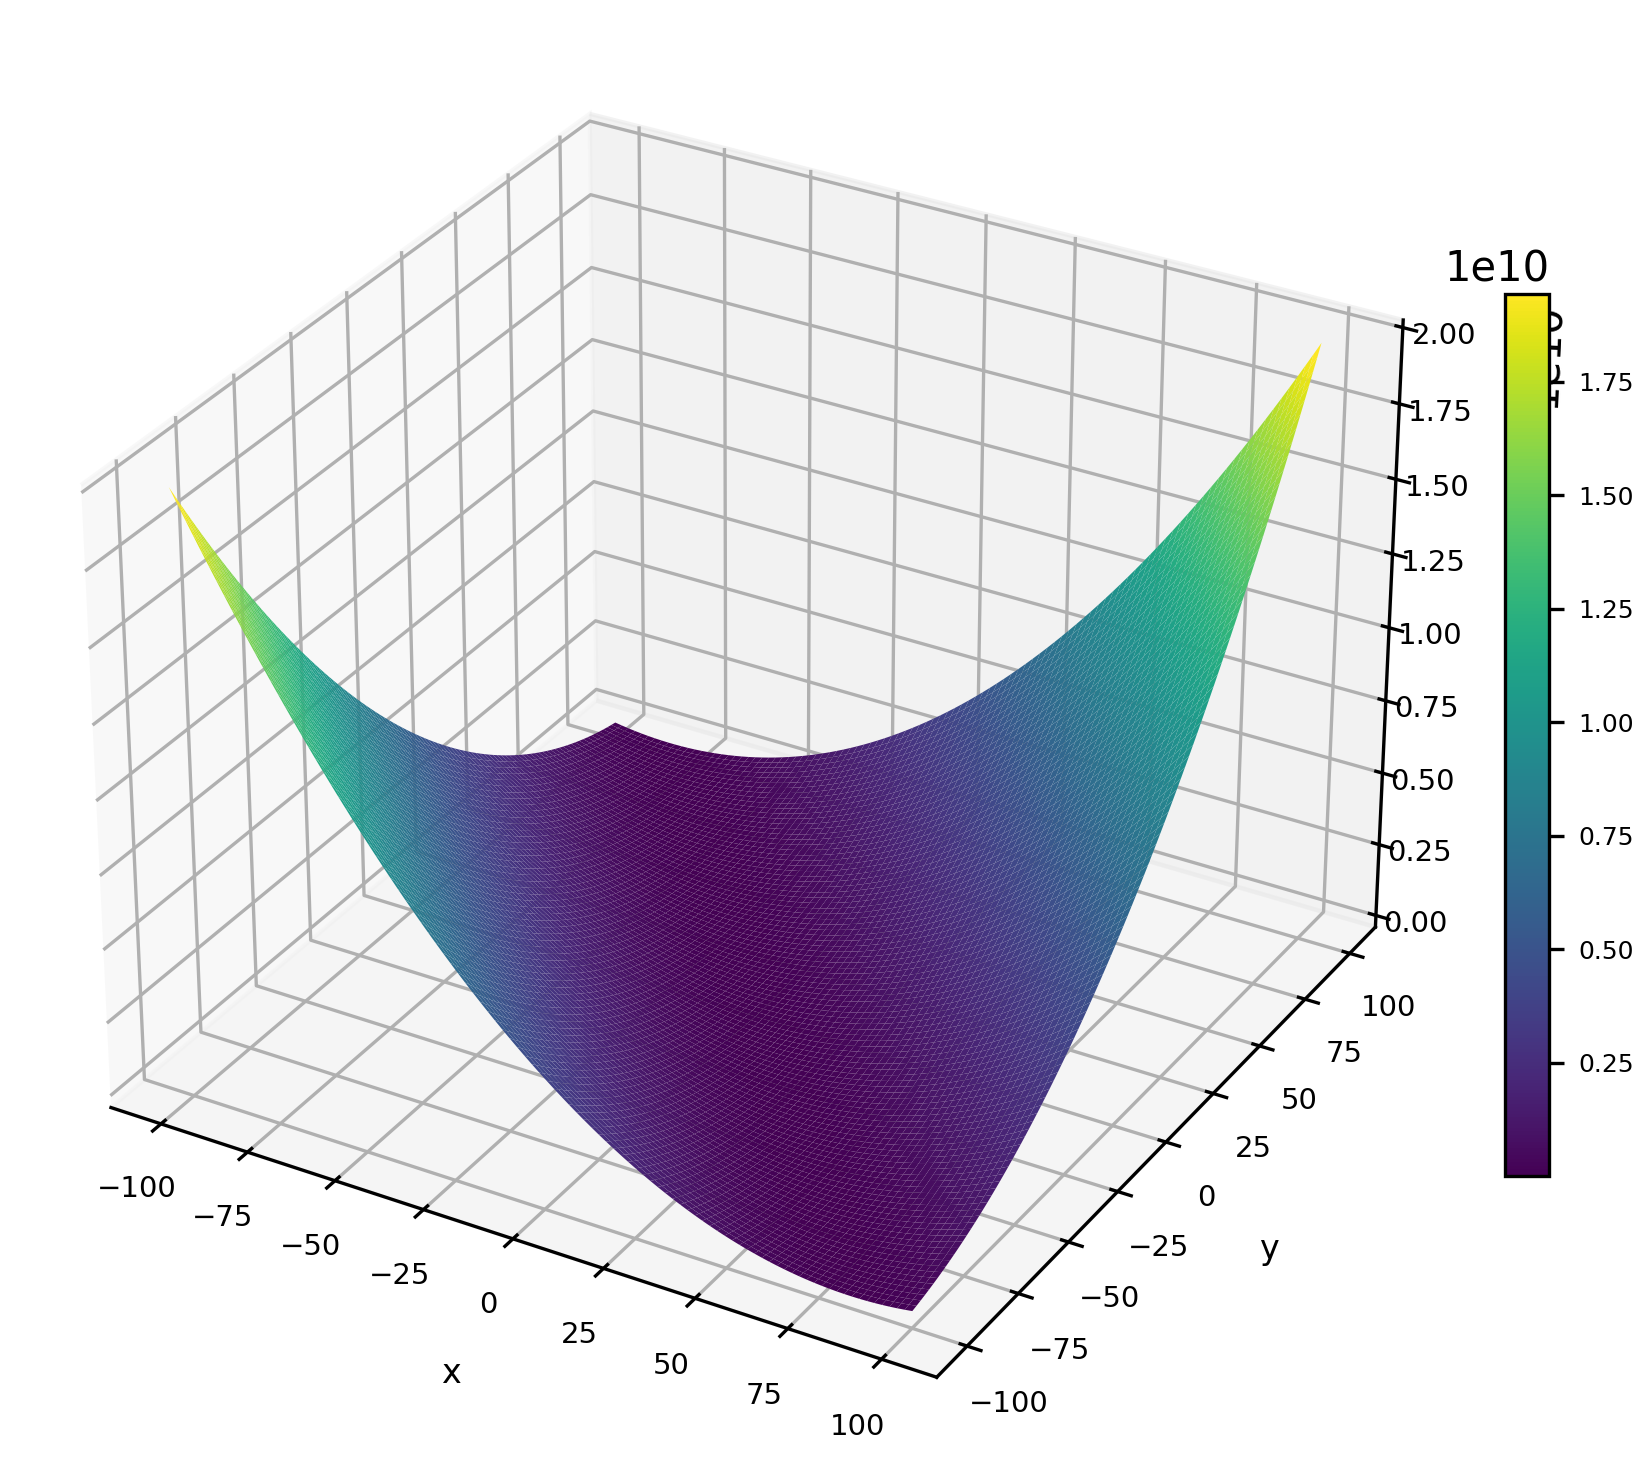
\includegraphics[width=1\textwidth]{Figures/benchmark_plots/Rotated_Bent_Cigar_maximized.png}
        \caption{Rotated Bent Cigar}
    \end{subfigure}
    % \hspace{.5cm} % Adjust the space as needed.
    \begin{subfigure}{0.32\textwidth}
        \centering
        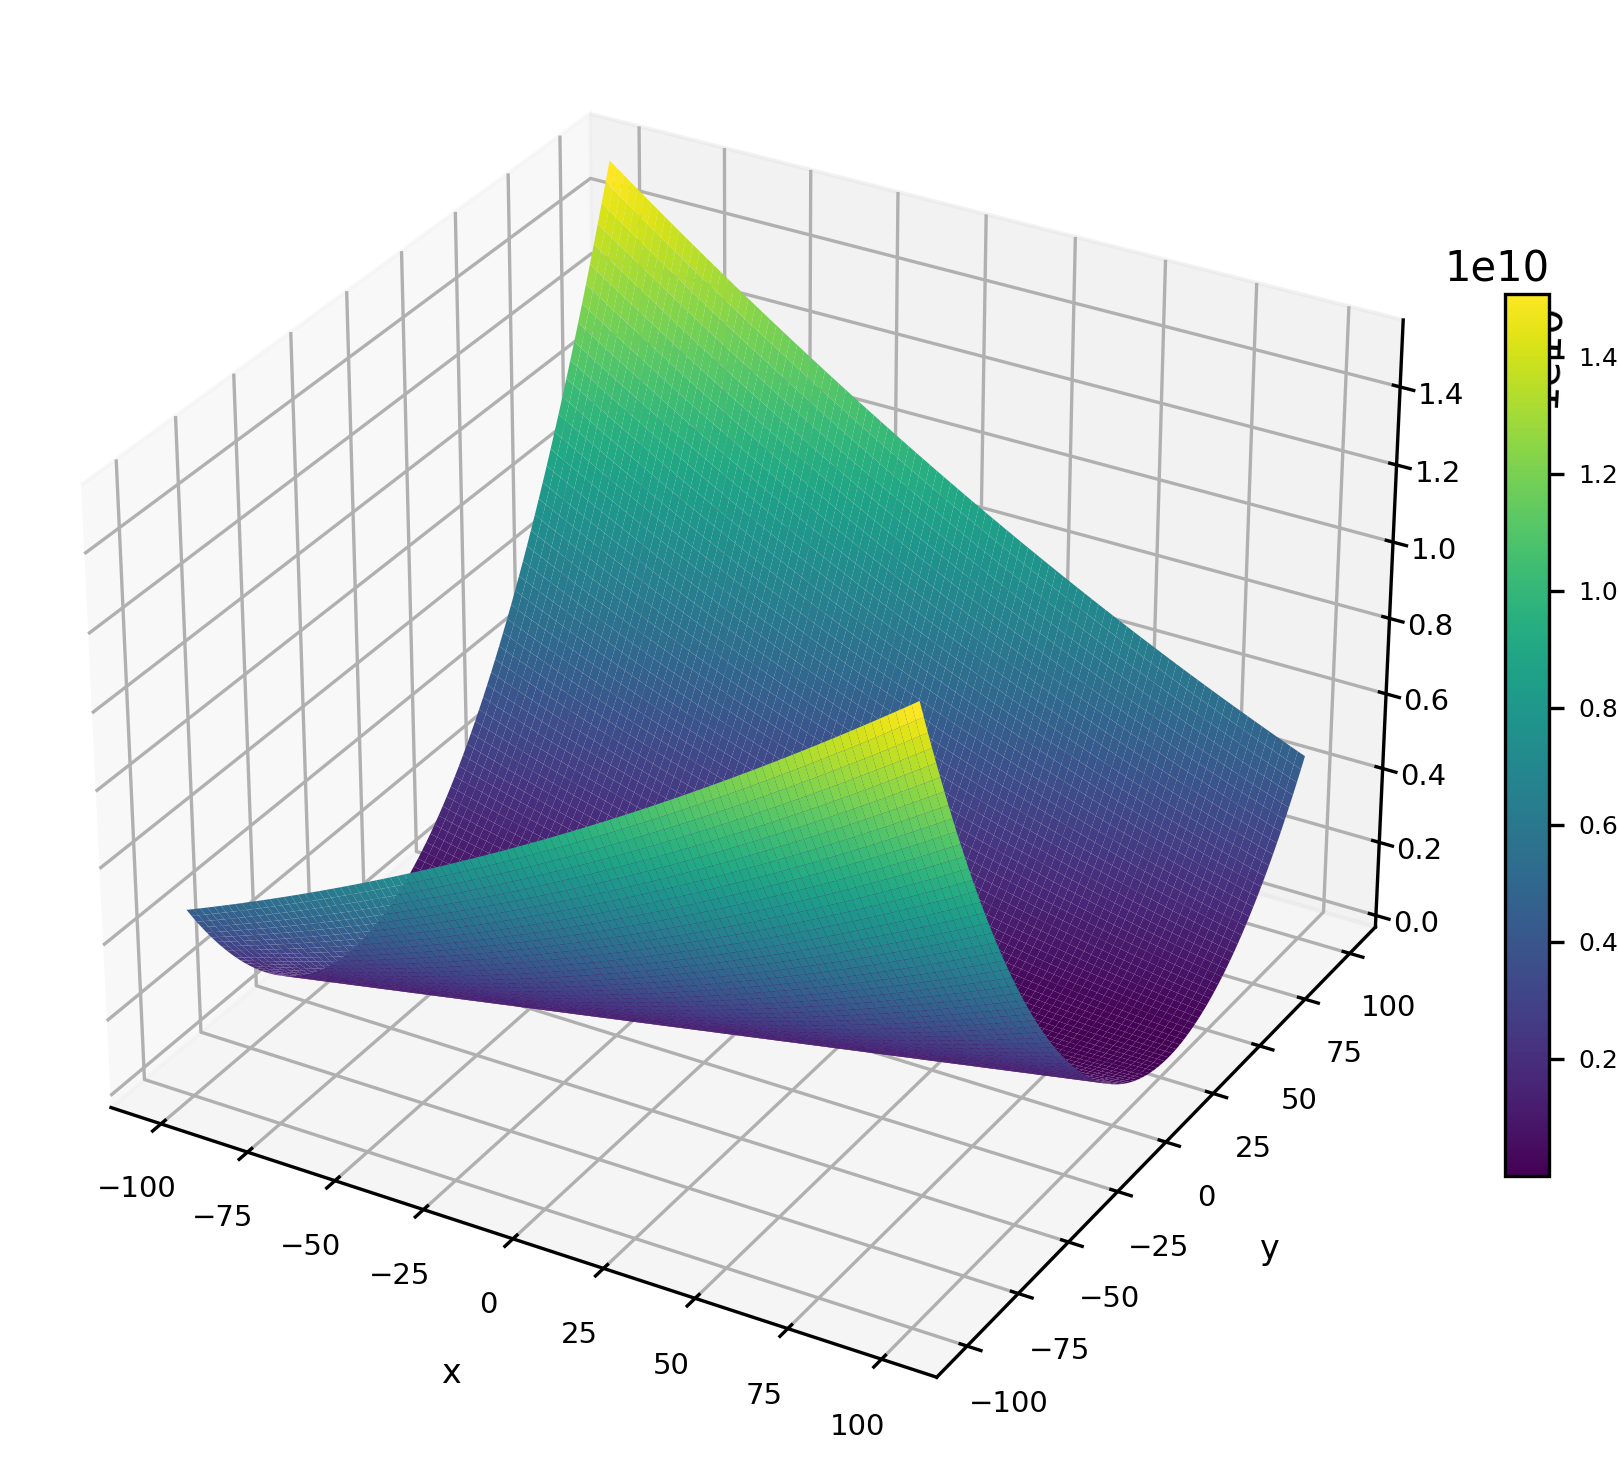
\includegraphics[width=1\textwidth]{Figures/benchmark_plots/Rotated_Discus_maximized.png}
        \caption{Rotated Discus}
    \end{subfigure}
        \begin{subfigure}{0.32\textwidth}
        \centering
        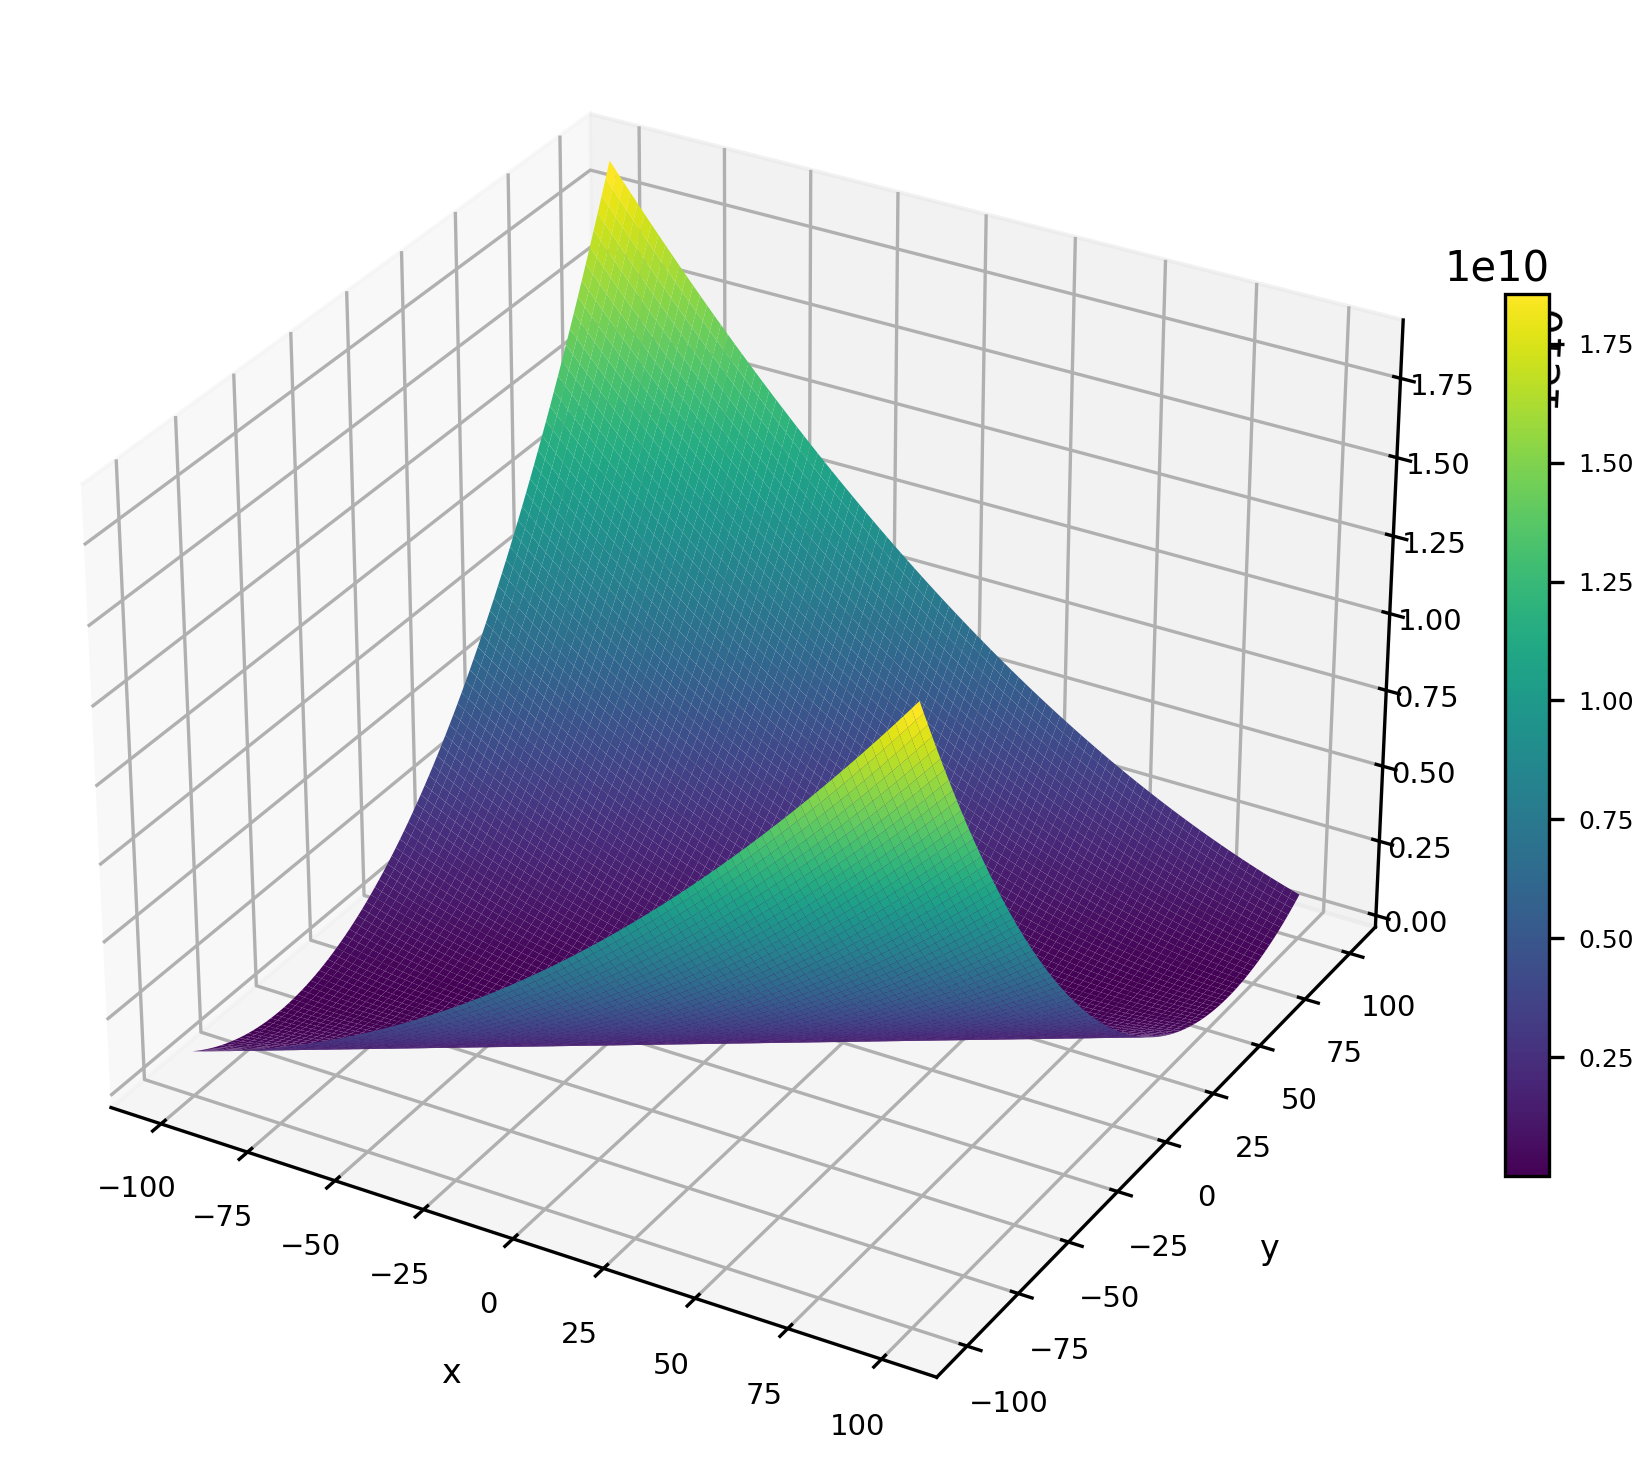
\includegraphics[width=1\textwidth]{Figures/benchmark_plots/Rotated_High_Conditioned_Elliptic_maximized.png}
        \caption{Rotated Elliptic}
    \end{subfigure}
    % \hspace{.5cm} % Adjust the space as needed.
    \begin{subfigure}{0.32\textwidth}
        \centering
        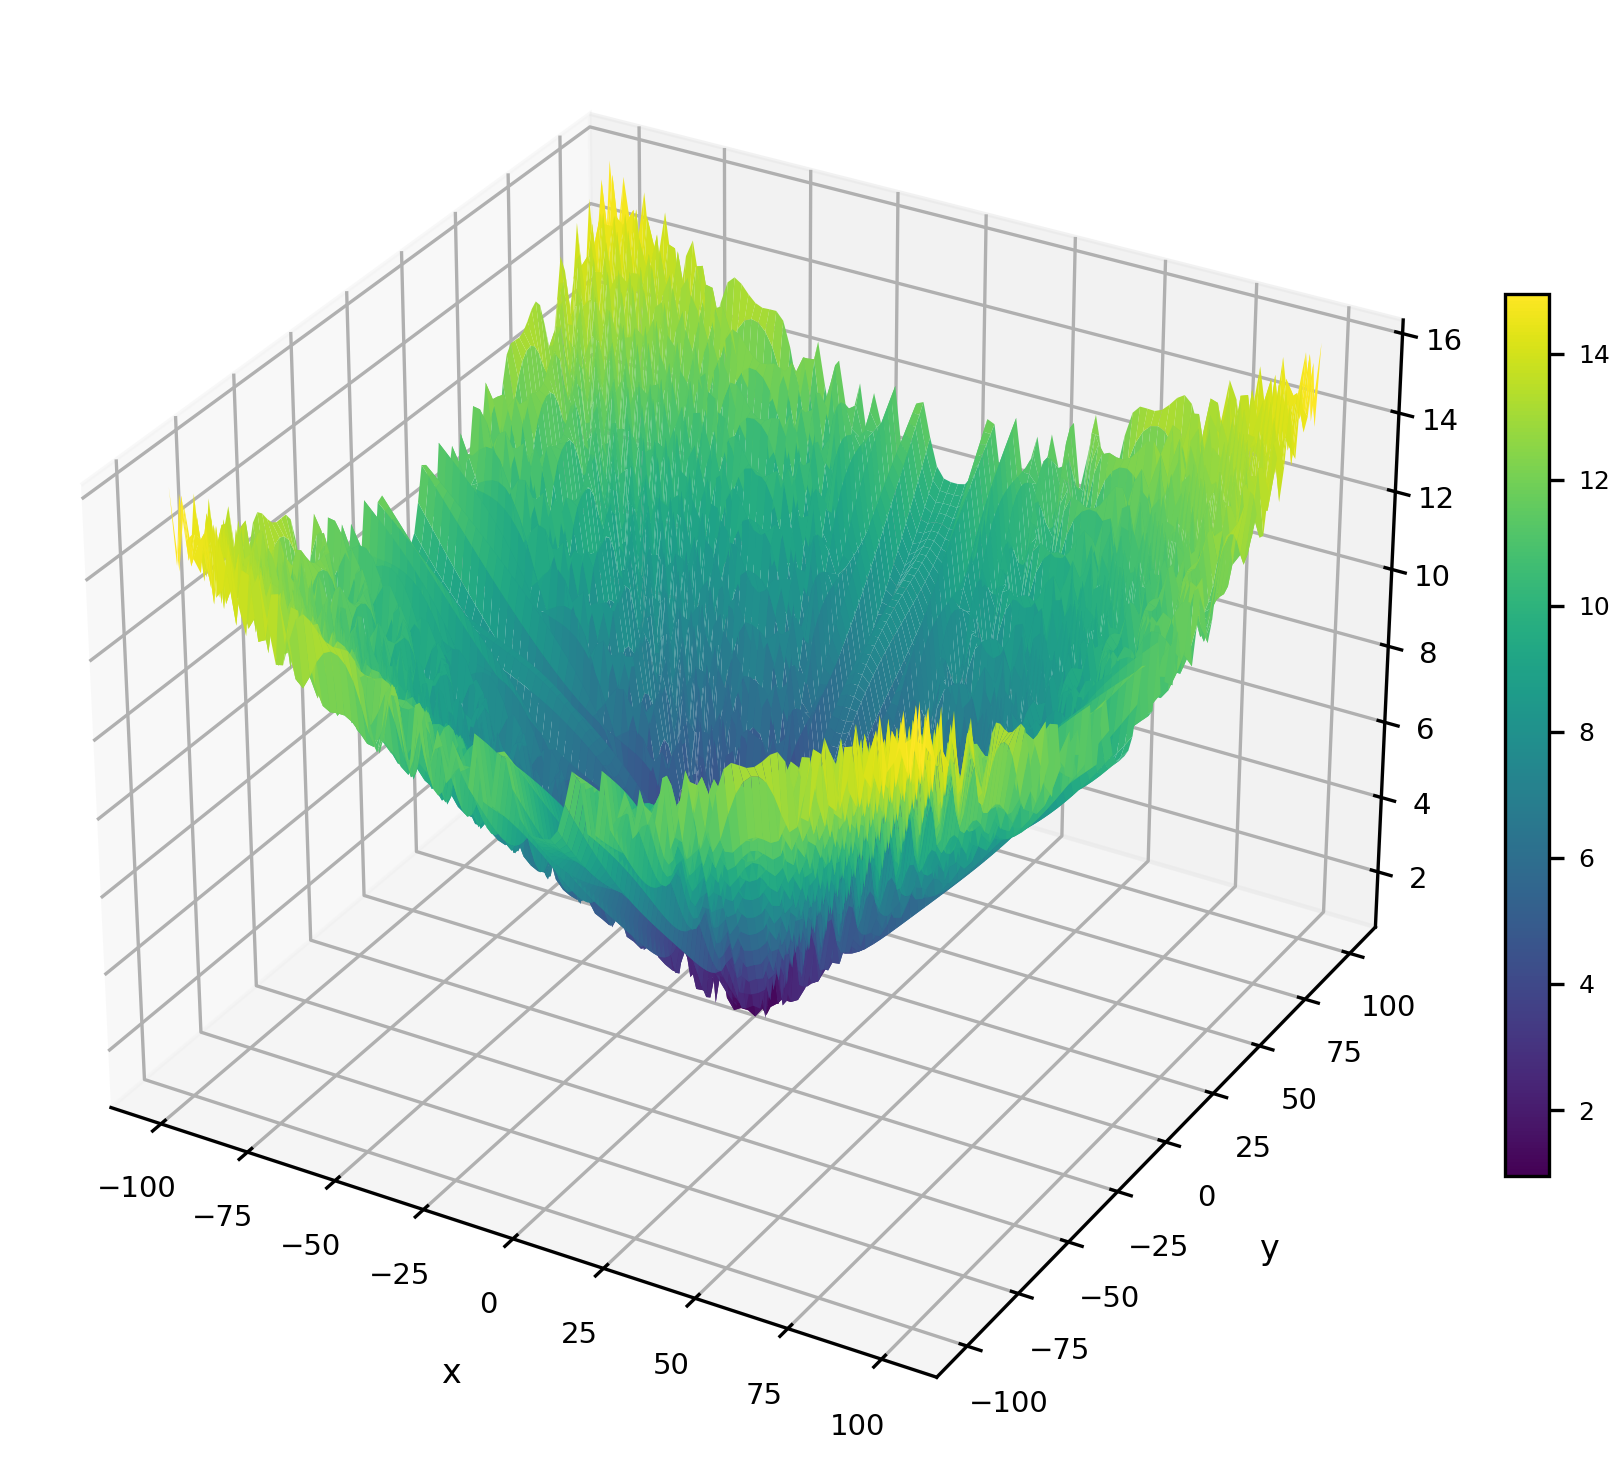
\includegraphics[width=1\textwidth]{Figures/benchmark_plots/Salomon_maximized.png}
        \caption{Salomon}
    \end{subfigure}
    \begin{subfigure}{0.32\textwidth}
        \centering
        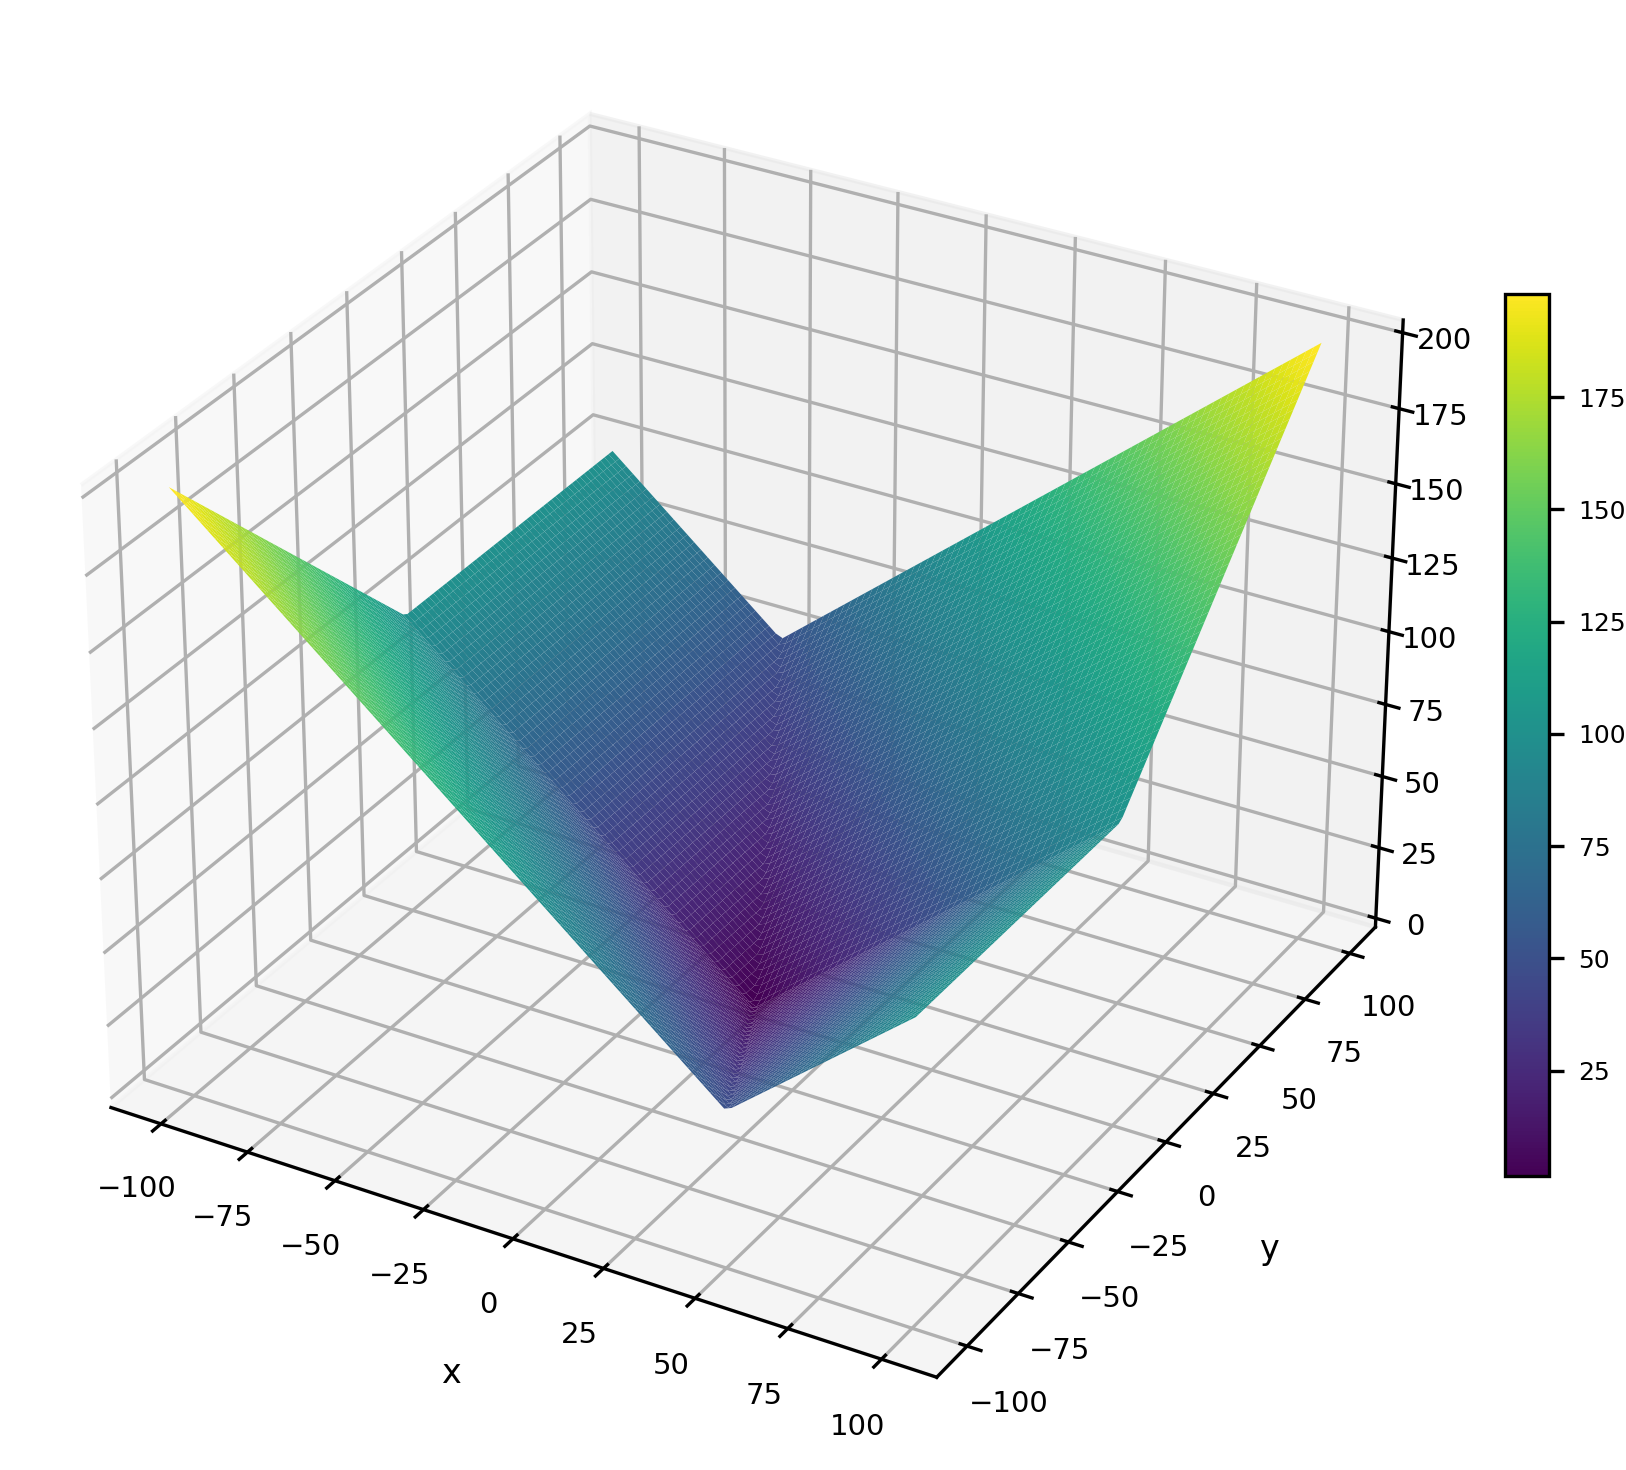
\includegraphics[width=1\textwidth]{Figures/benchmark_plots/Schwefel_N20_maximized.png}
        \caption{Schwefel N.2.0}
    \end{subfigure}
    % \hspace{.5cm} % Adjust the space as needed.
    \begin{subfigure}{0.32\textwidth}
        \centering
        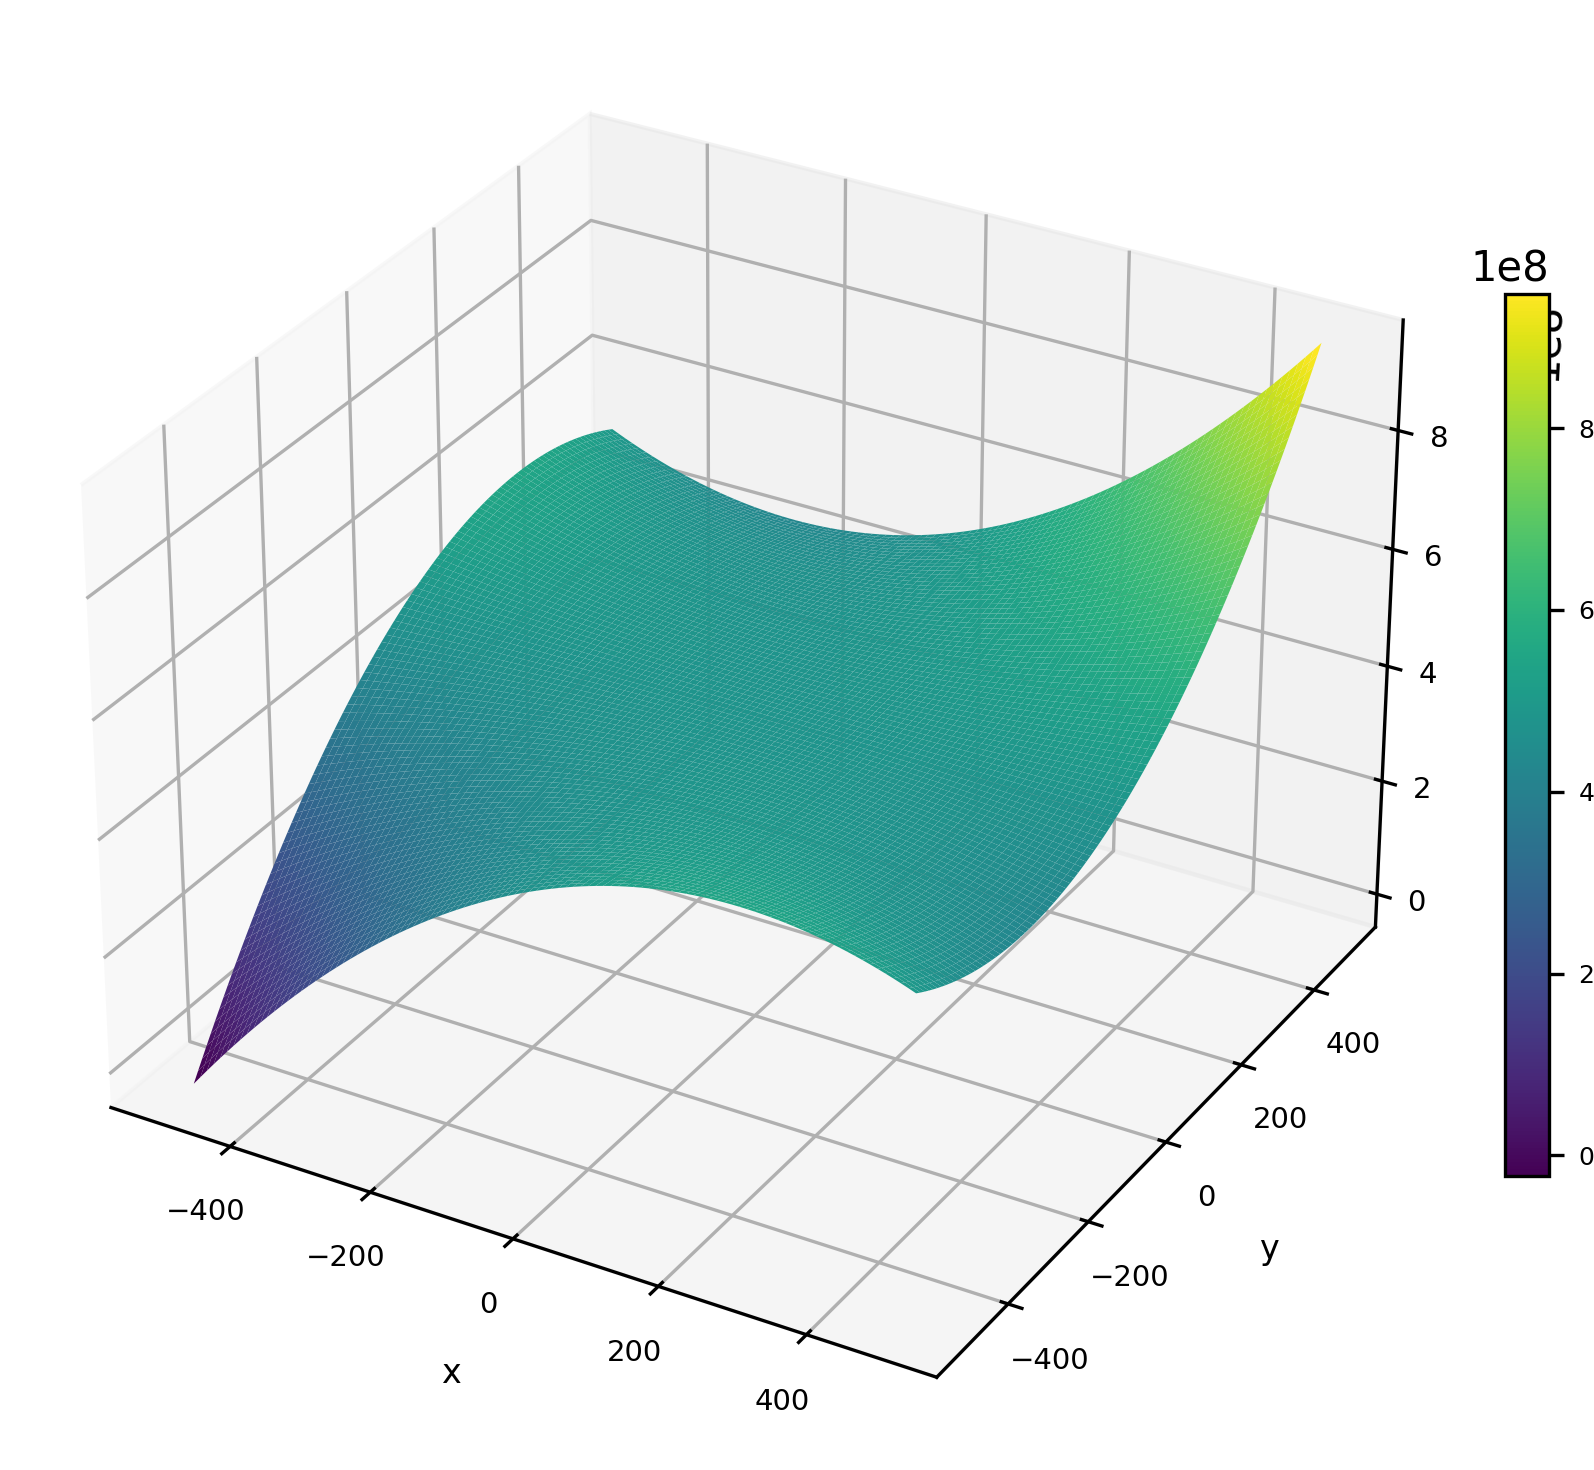
\includegraphics[width=1\textwidth]{Figures/benchmark_plots/Schwefel_N36_maximized.png}
        \caption{Schwefel N.3.6}
    \end{subfigure}
        \captionsetup{list=no}
\caption{Two-dimensional visualizations of benchmark problem landscapes.}
\end{figure}

\begin{figure}[p]\ContinuedFloat
\renewcommand\thesubfigure{A.\arabic{subfigure}} % Local change starts here
    \centering
    \begin{subfigure}{0.32\textwidth}
        \centering
        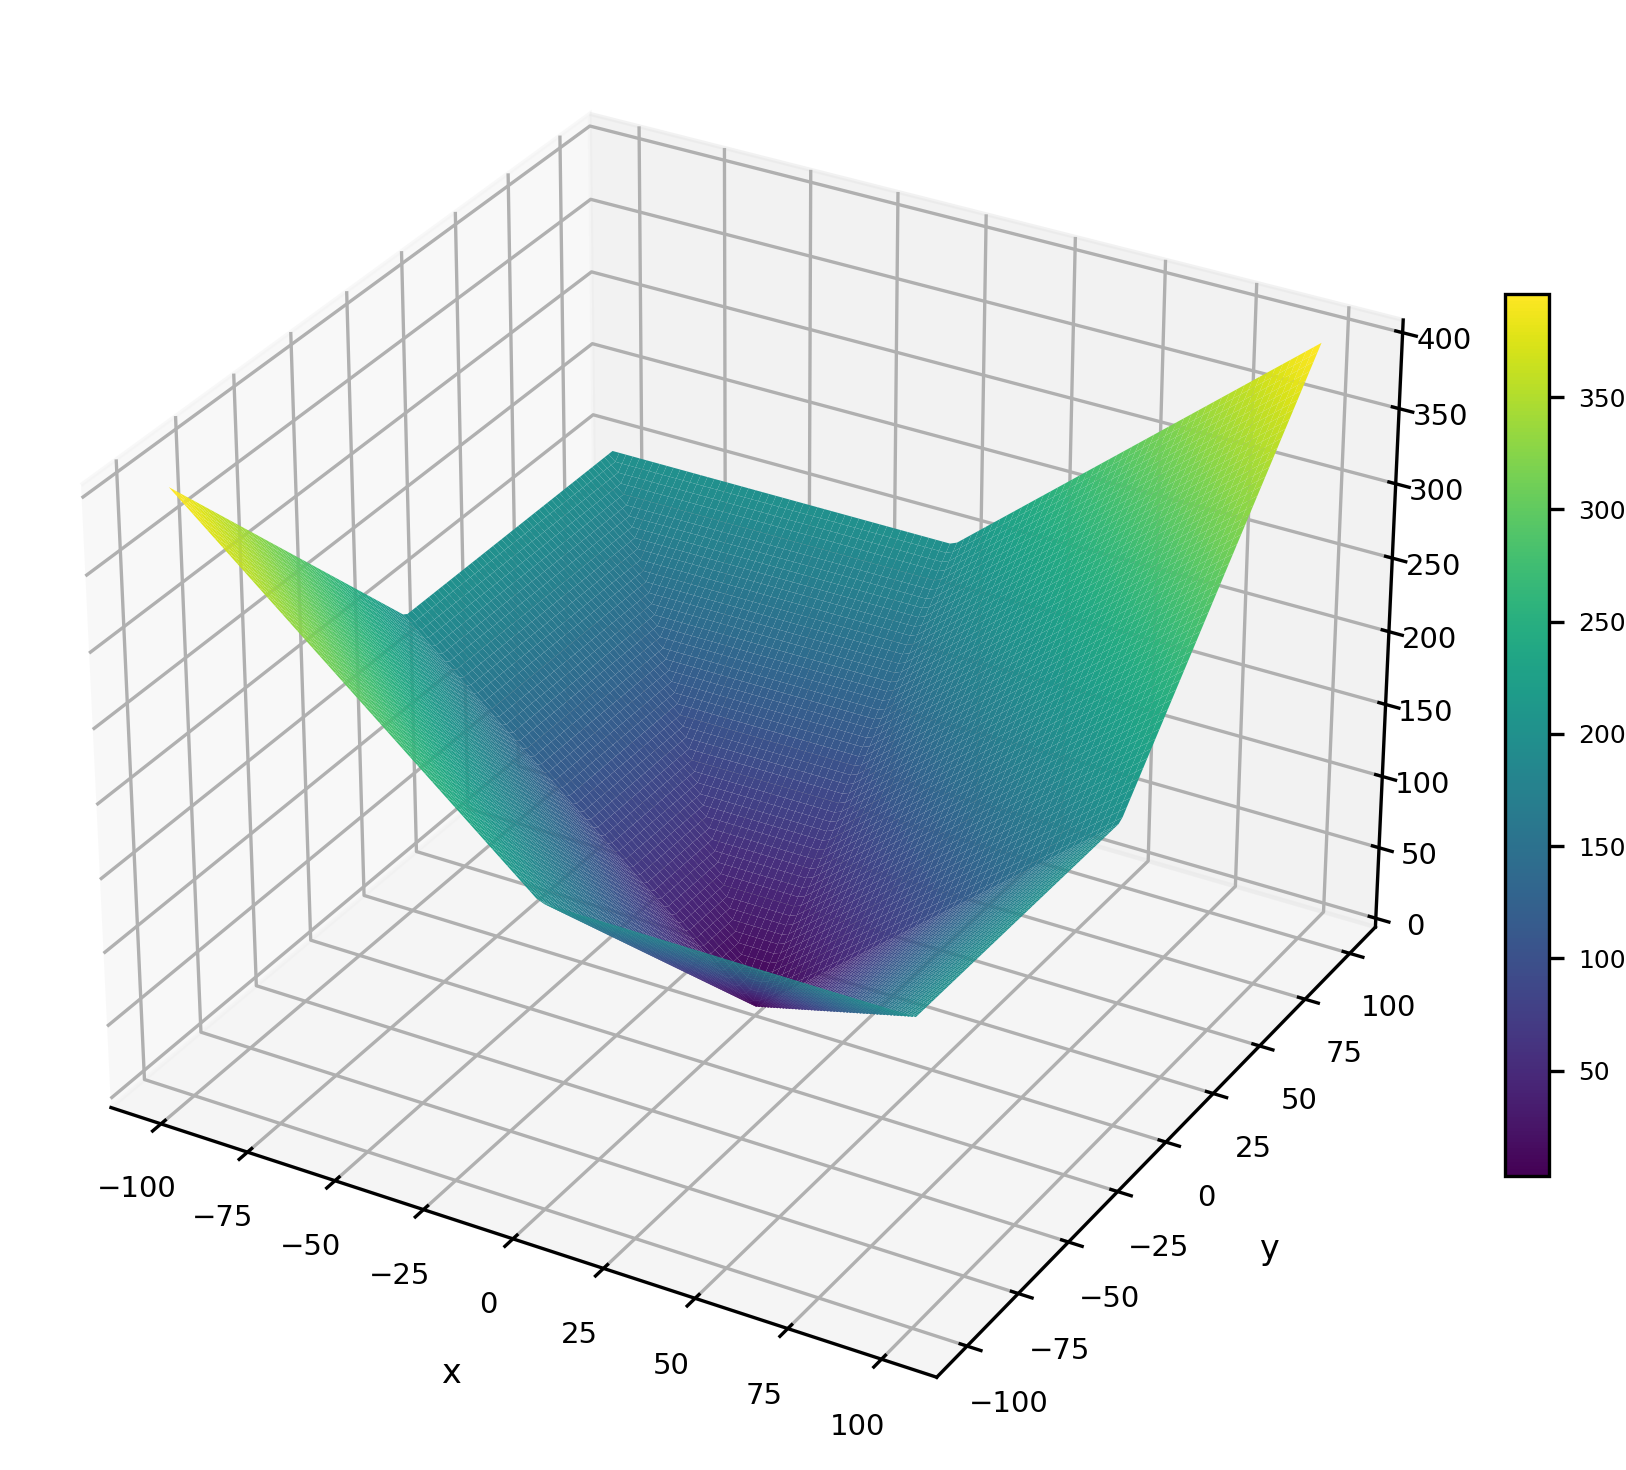
\includegraphics[width=1\textwidth]{Figures/benchmark_plots/Schwefel_N6_maximized.png}
        \caption{Schwefel N.6}
    \end{subfigure}
    % \hspace{.5cm} % Adjust the space as needed.
    \begin{subfigure}{0.32\textwidth}
        \centering
        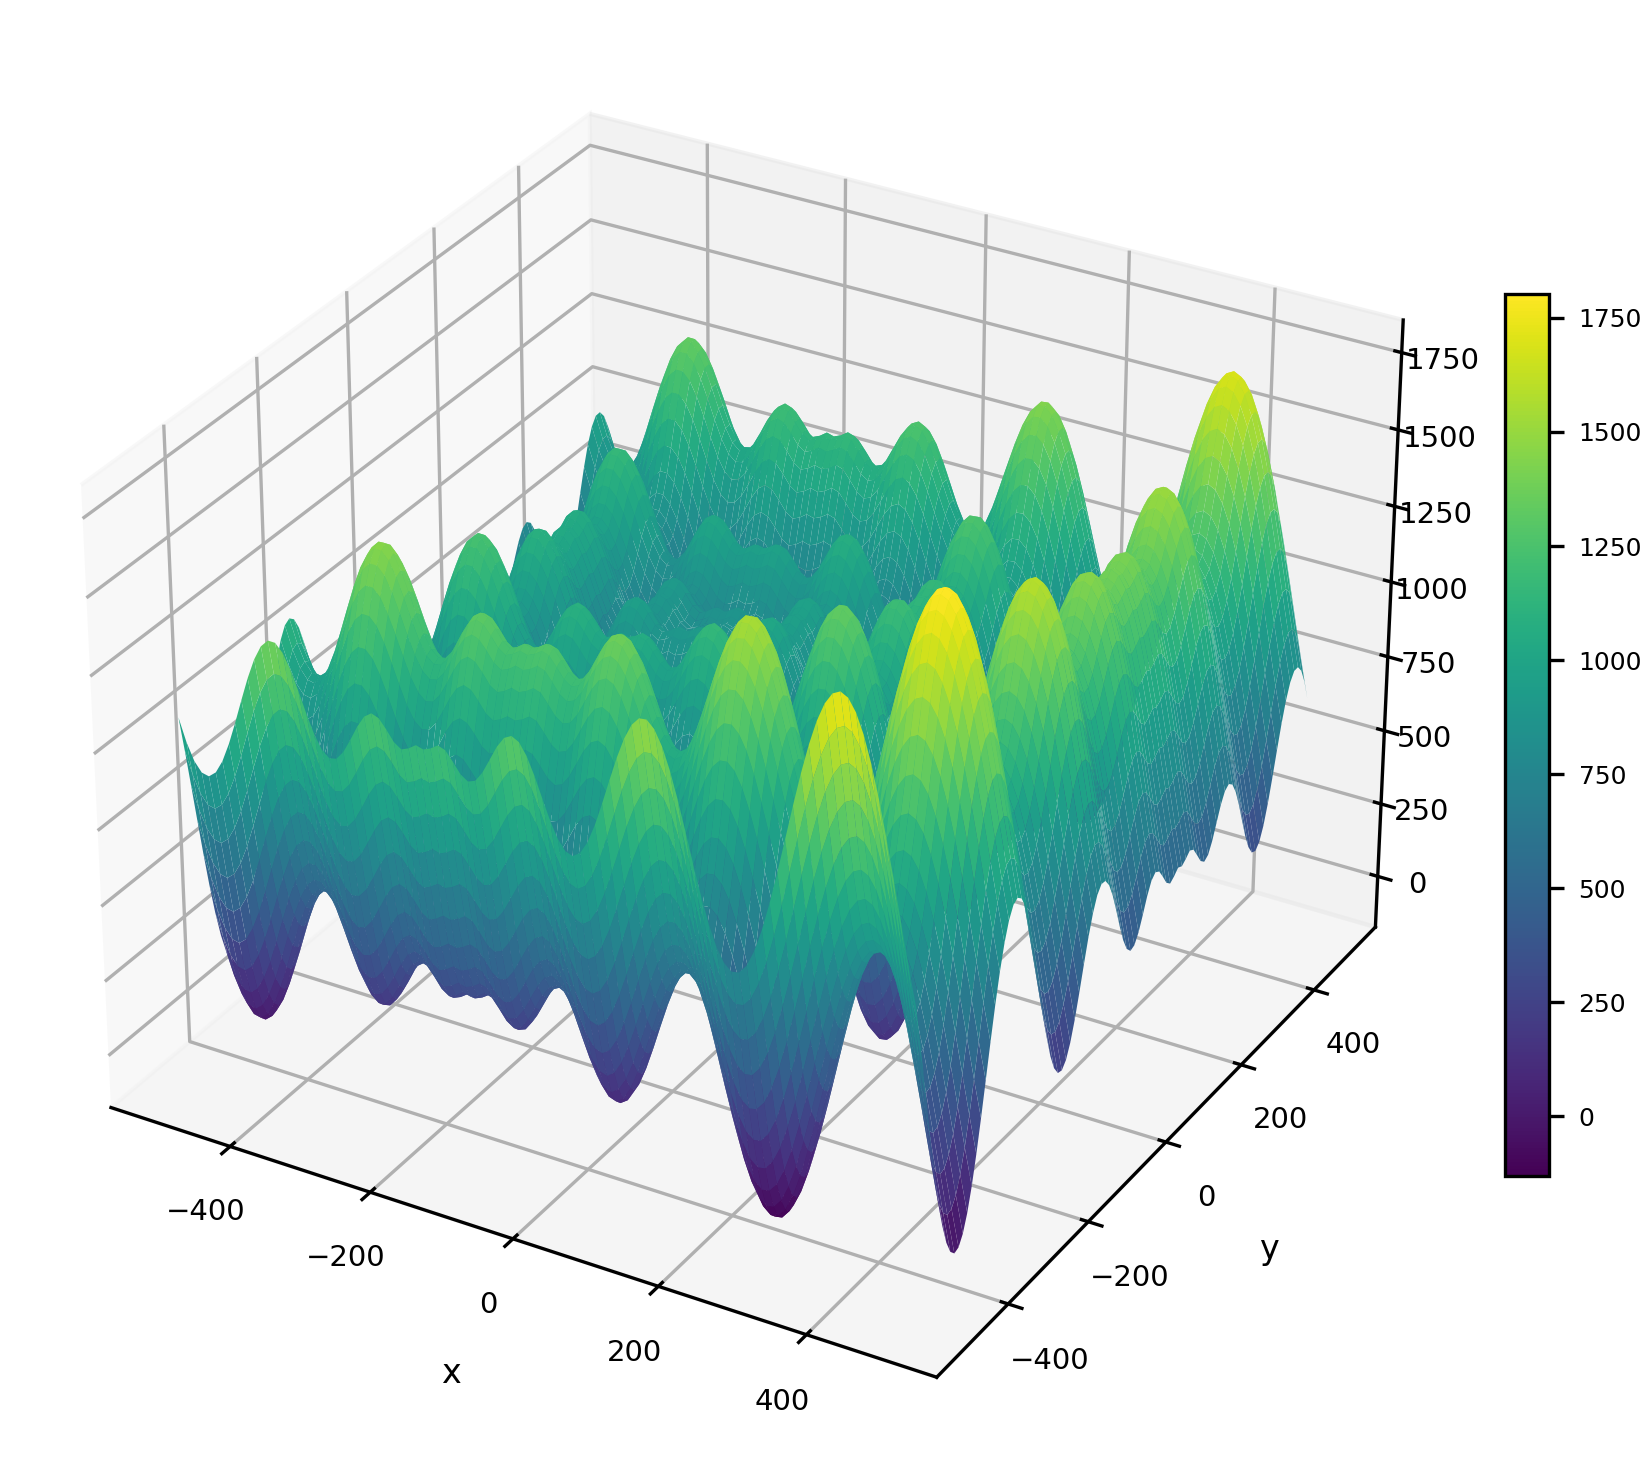
\includegraphics[width=1\textwidth]{Figures/benchmark_plots/Shifted_Schwefel_maximized.png}
        \caption{Shifted Schwefel (N.2.6)}
    \end{subfigure}
    \begin{subfigure}{0.32\textwidth}
        \centering
        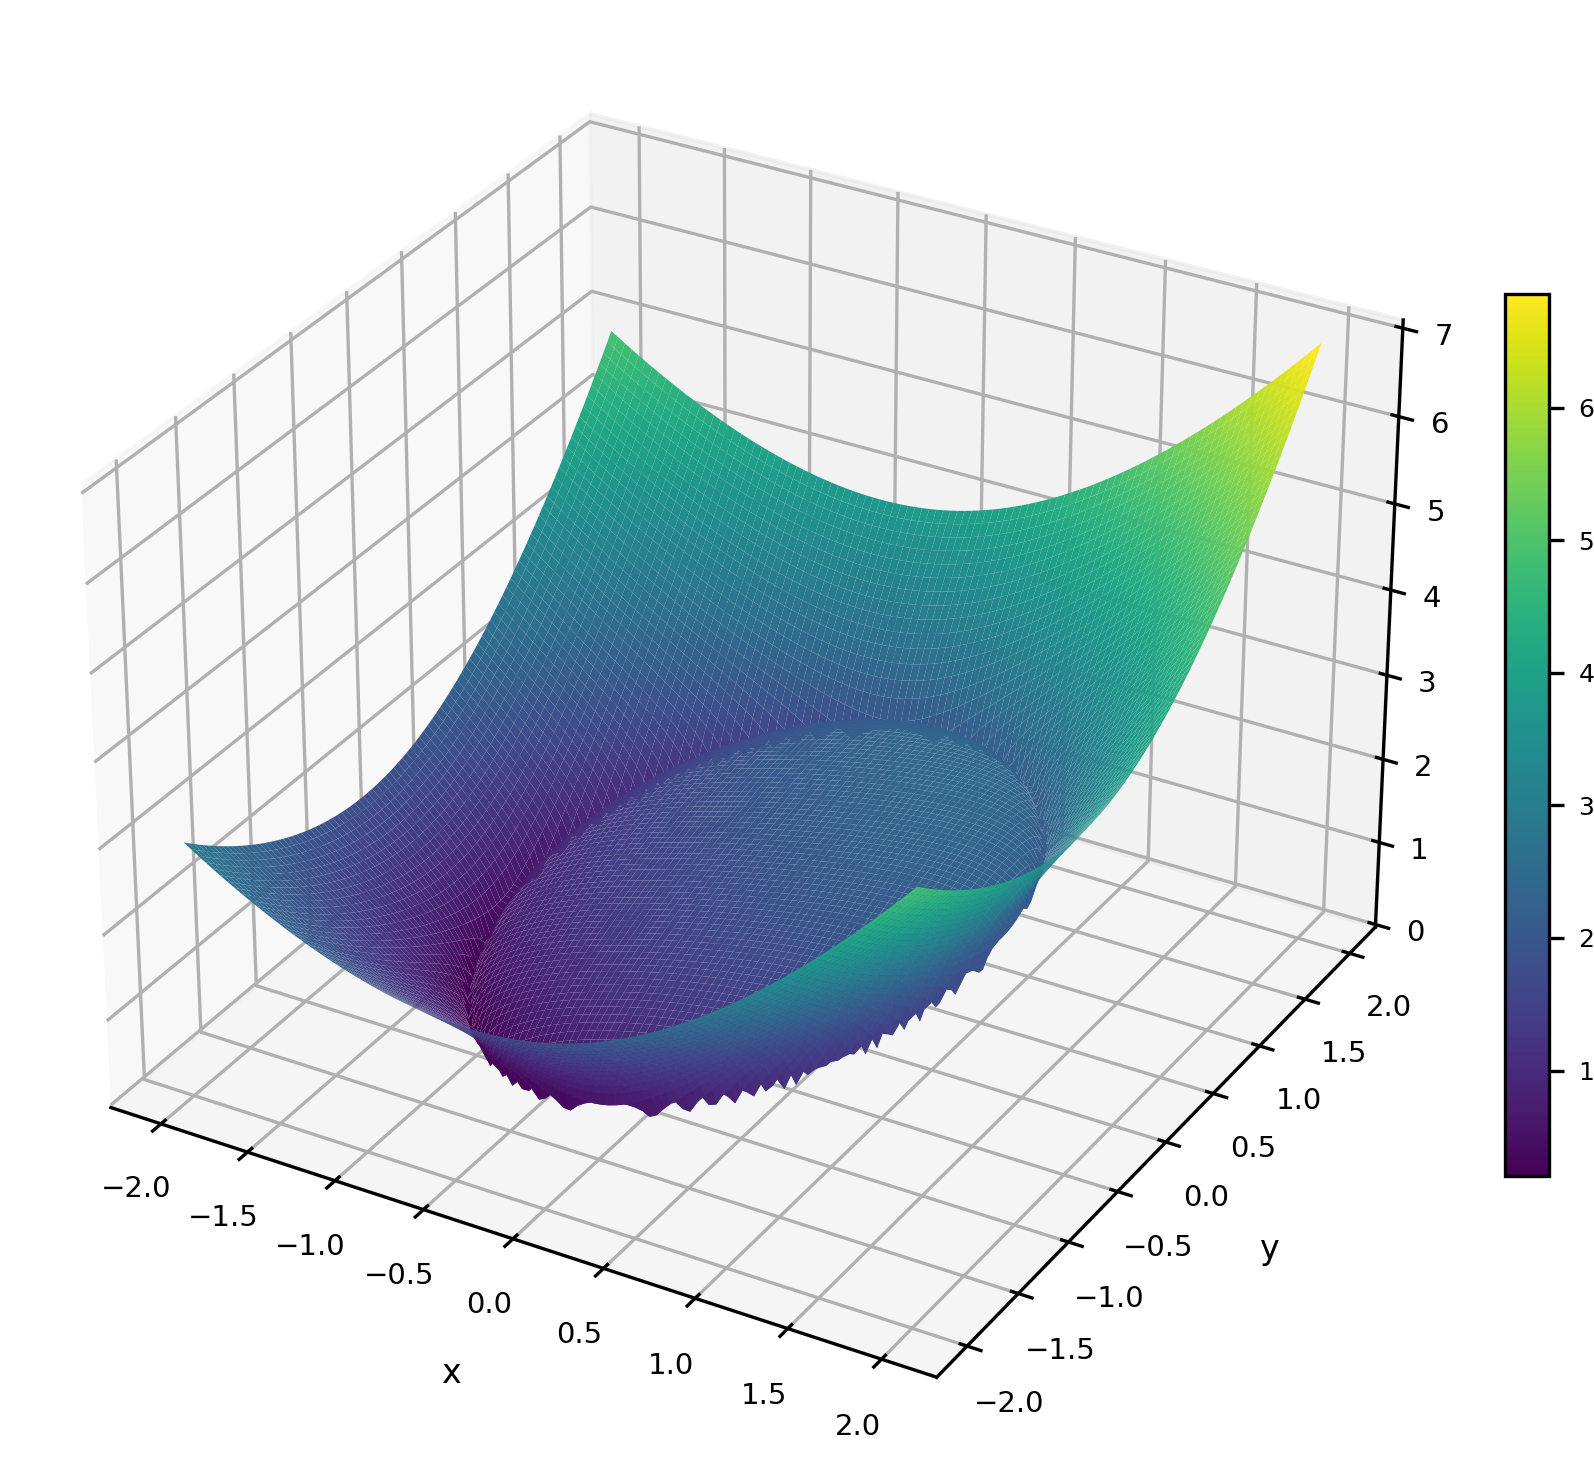
\includegraphics[width=1\textwidth]{Figures/benchmark_plots/Happy_Cat_maximized.png}
        \caption{HappyCat}
    \end{subfigure}
    % % \hspace{.5cm} % Adjust the space as needed.
    \begin{subfigure}{0.32\textwidth}
        \centering
        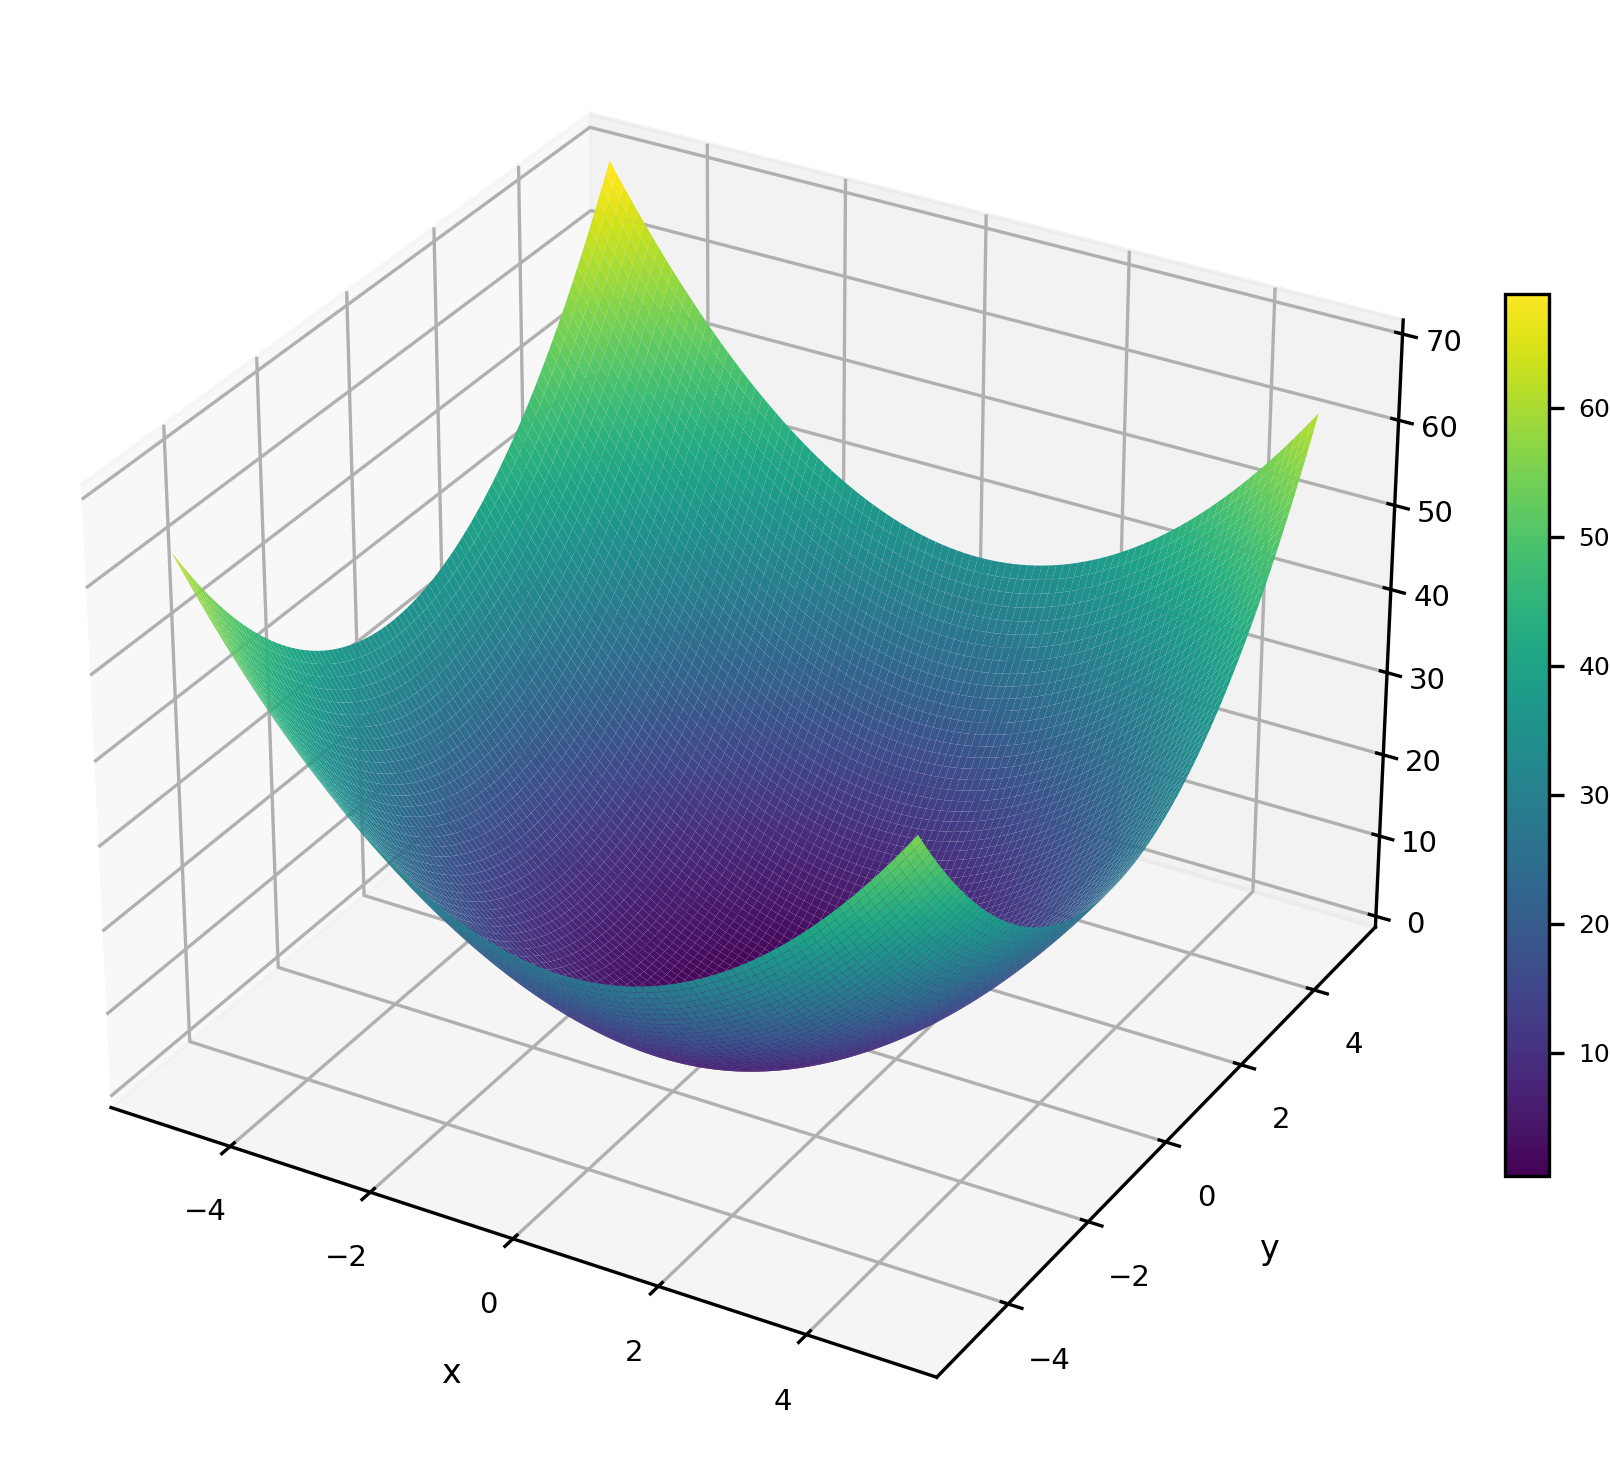
\includegraphics[width=1\textwidth]{Figures/benchmark_plots/Shifted_and_Rotated_HGBat_maximized.png}
        \caption{HGBat}
    \end{subfigure}
        \begin{subfigure}{0.32\textwidth}
        \centering
        \includegraphics[width=1\textwidth]{Figures/benchmark_plots/Shifted_and_Rotated_Expanded_Scaffer’s_F6_maximized.png}
        \caption{Schaffer F7}
    \end{subfigure}
        \begin{subfigure}{0.32\textwidth}
        \centering
        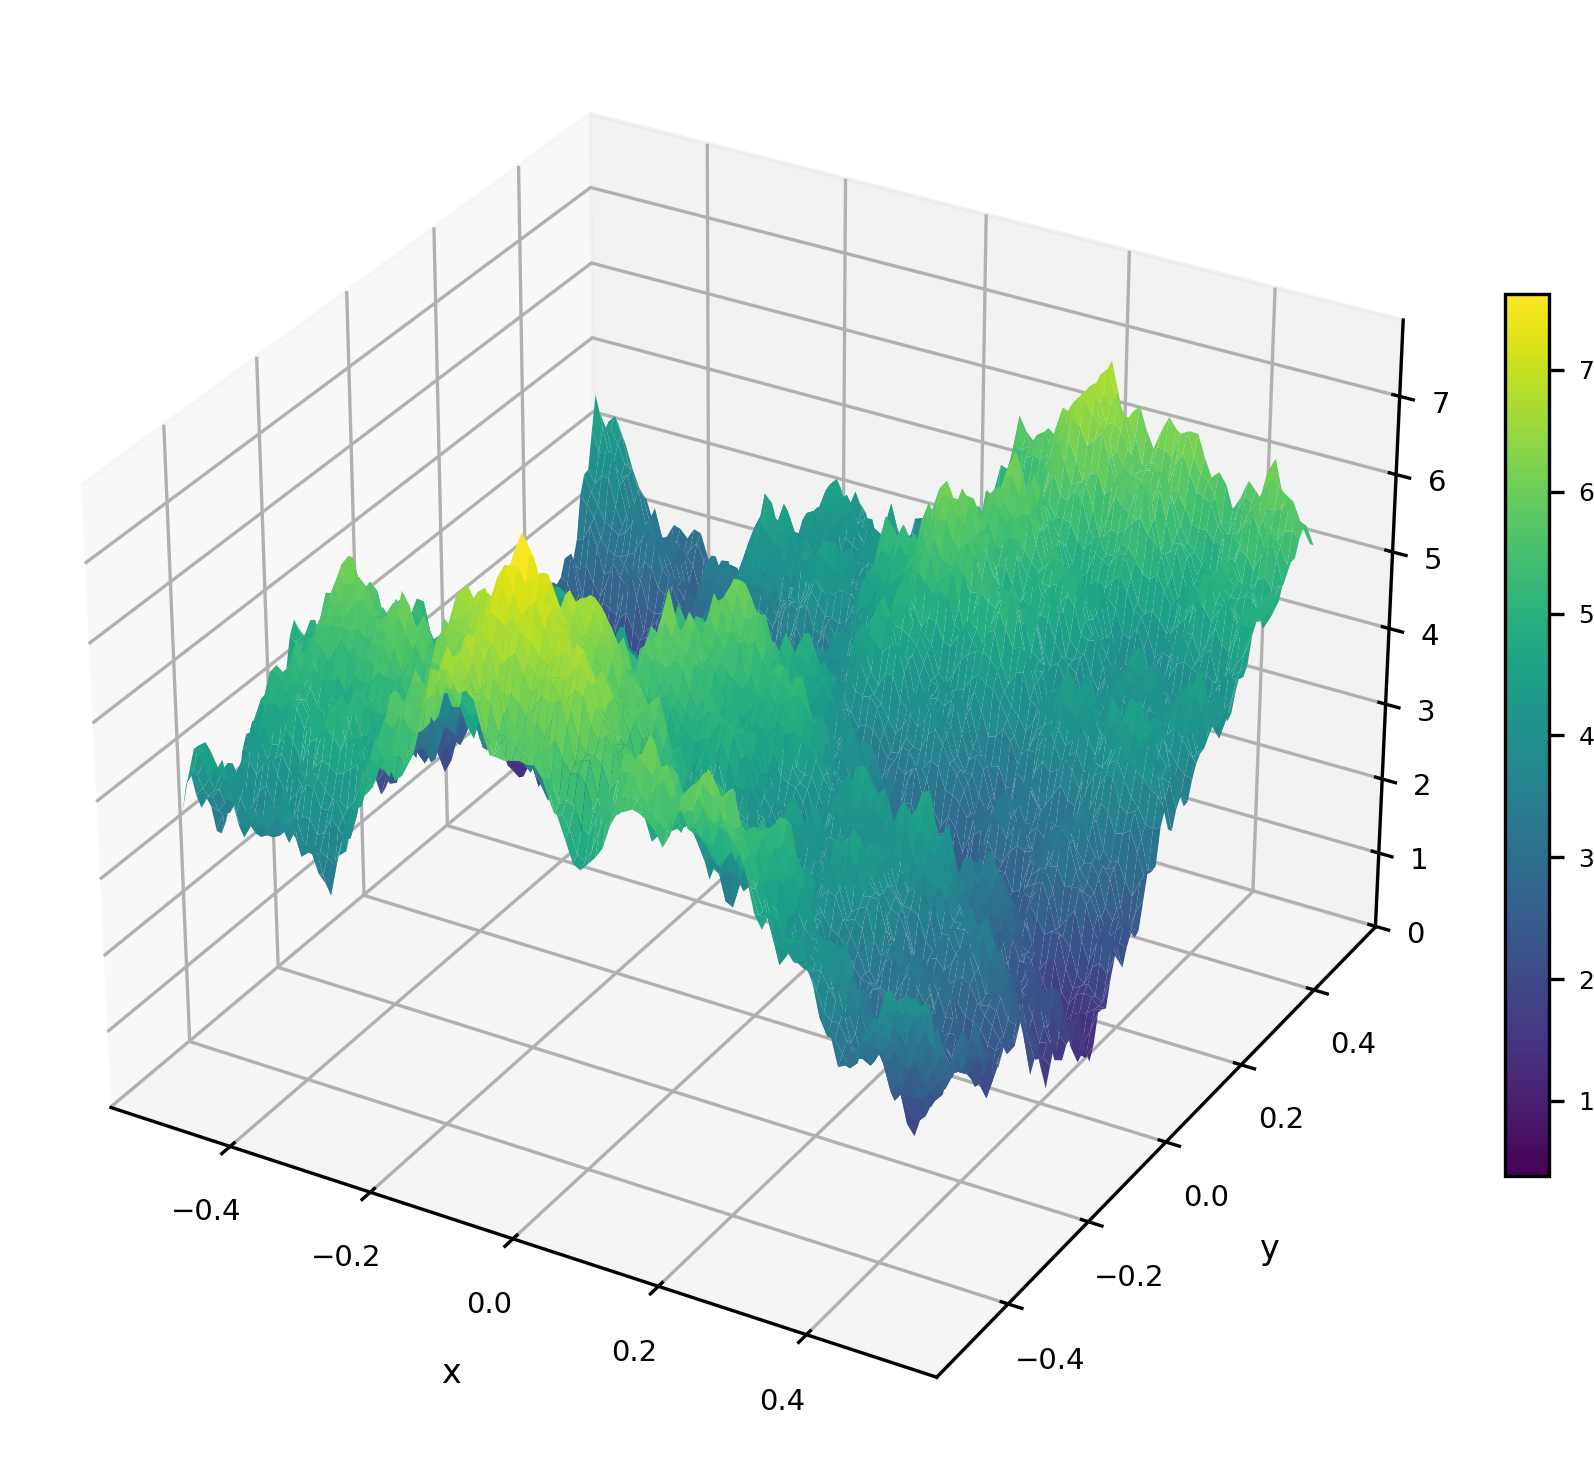
\includegraphics[width=1\textwidth]{Figures/benchmark_plots/Shifted_and_Rotated_Weierstrass_maximized.png}
        \caption{Weierstrass}
    \end{subfigure}
    % \hspace{.5cm} % Adjust the space as needed.
    \begin{subfigure}{0.32\textwidth}
        \centering
        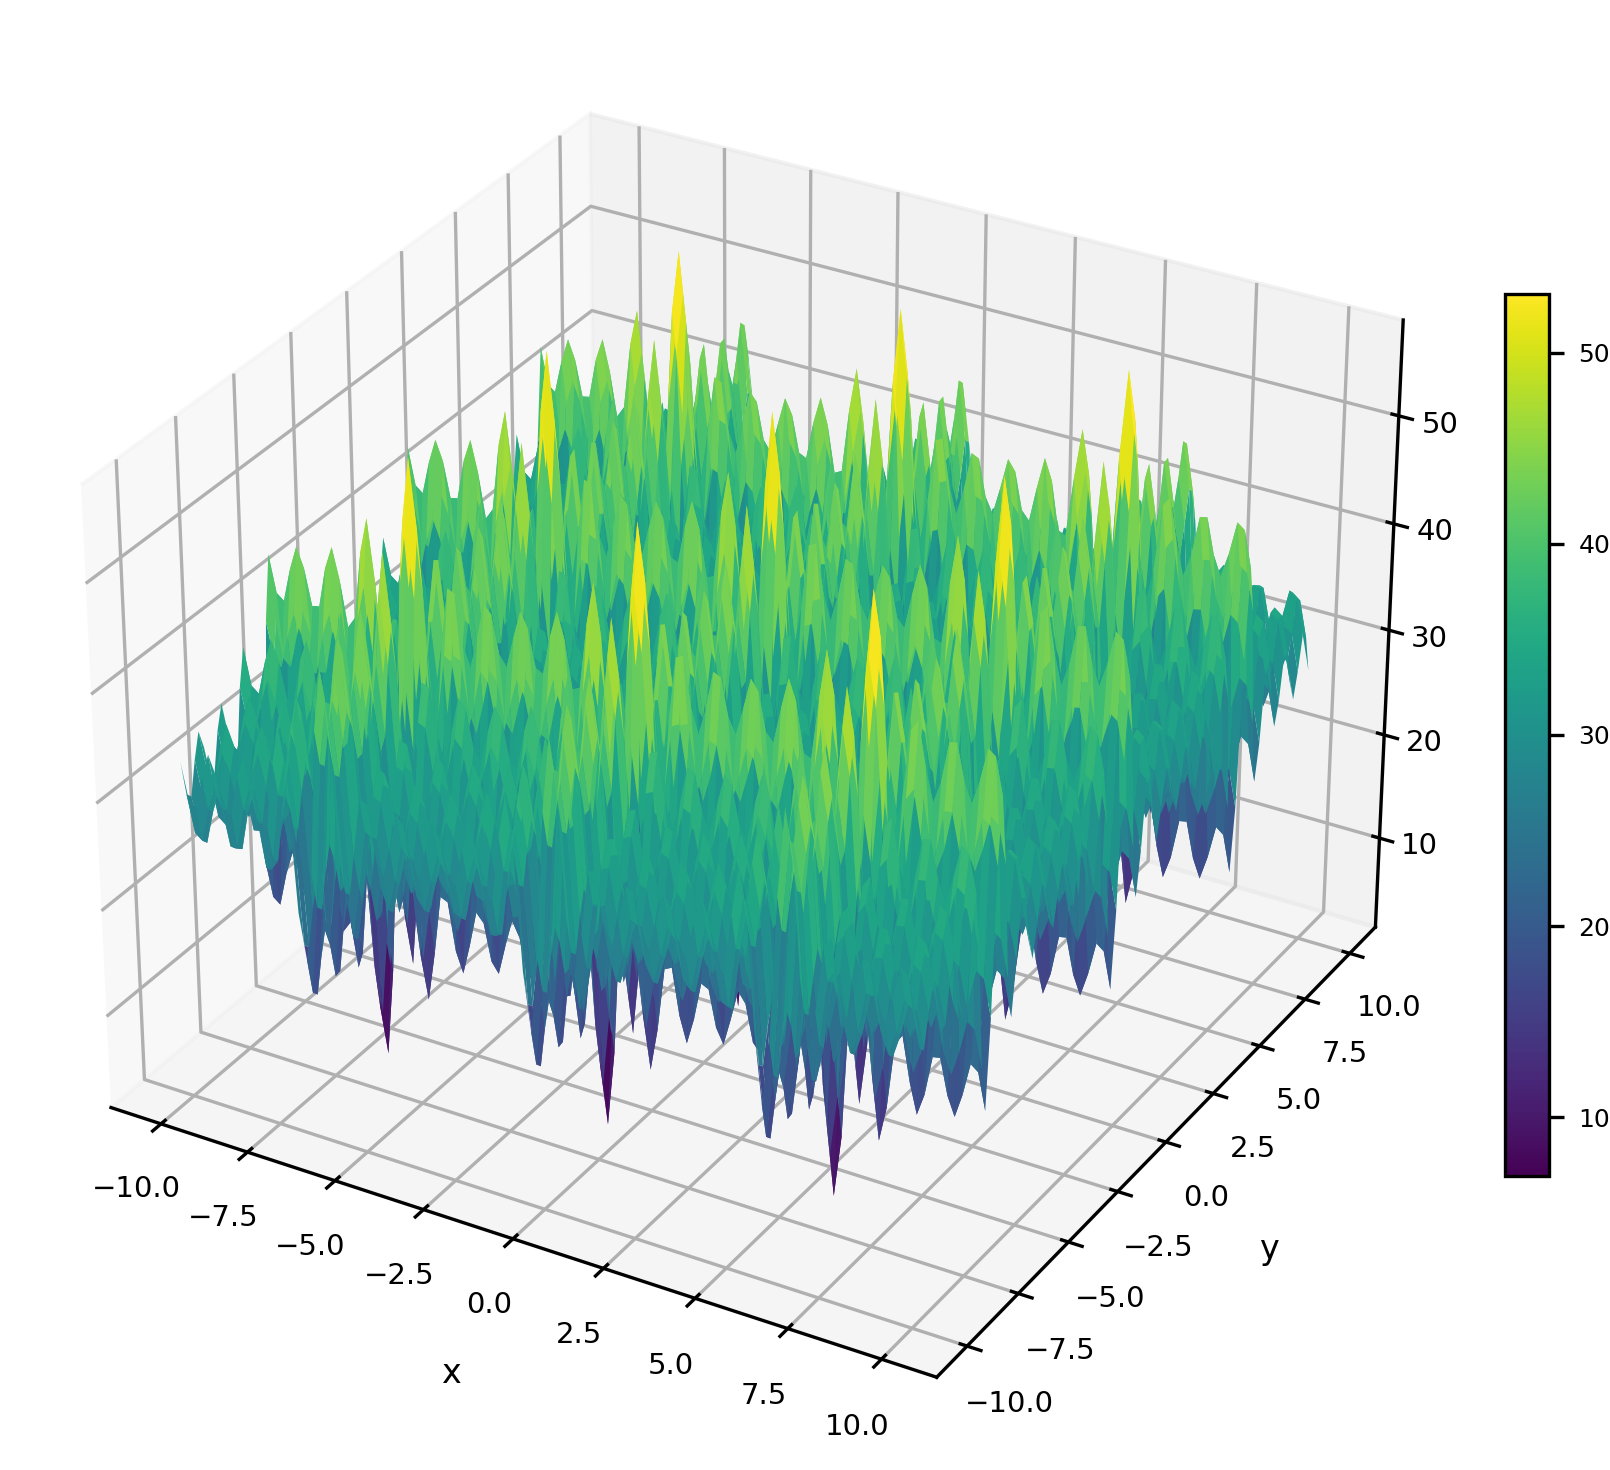
\includegraphics[width=1\textwidth]{Figures/benchmark_plots/Shubert_N3_maximized.png}
        \caption{Shubert N.3}
    \end{subfigure}
    % \hspace{.5cm} % Adjust the space as needed.
    \begin{subfigure}{0.32\textwidth}
        \centering
        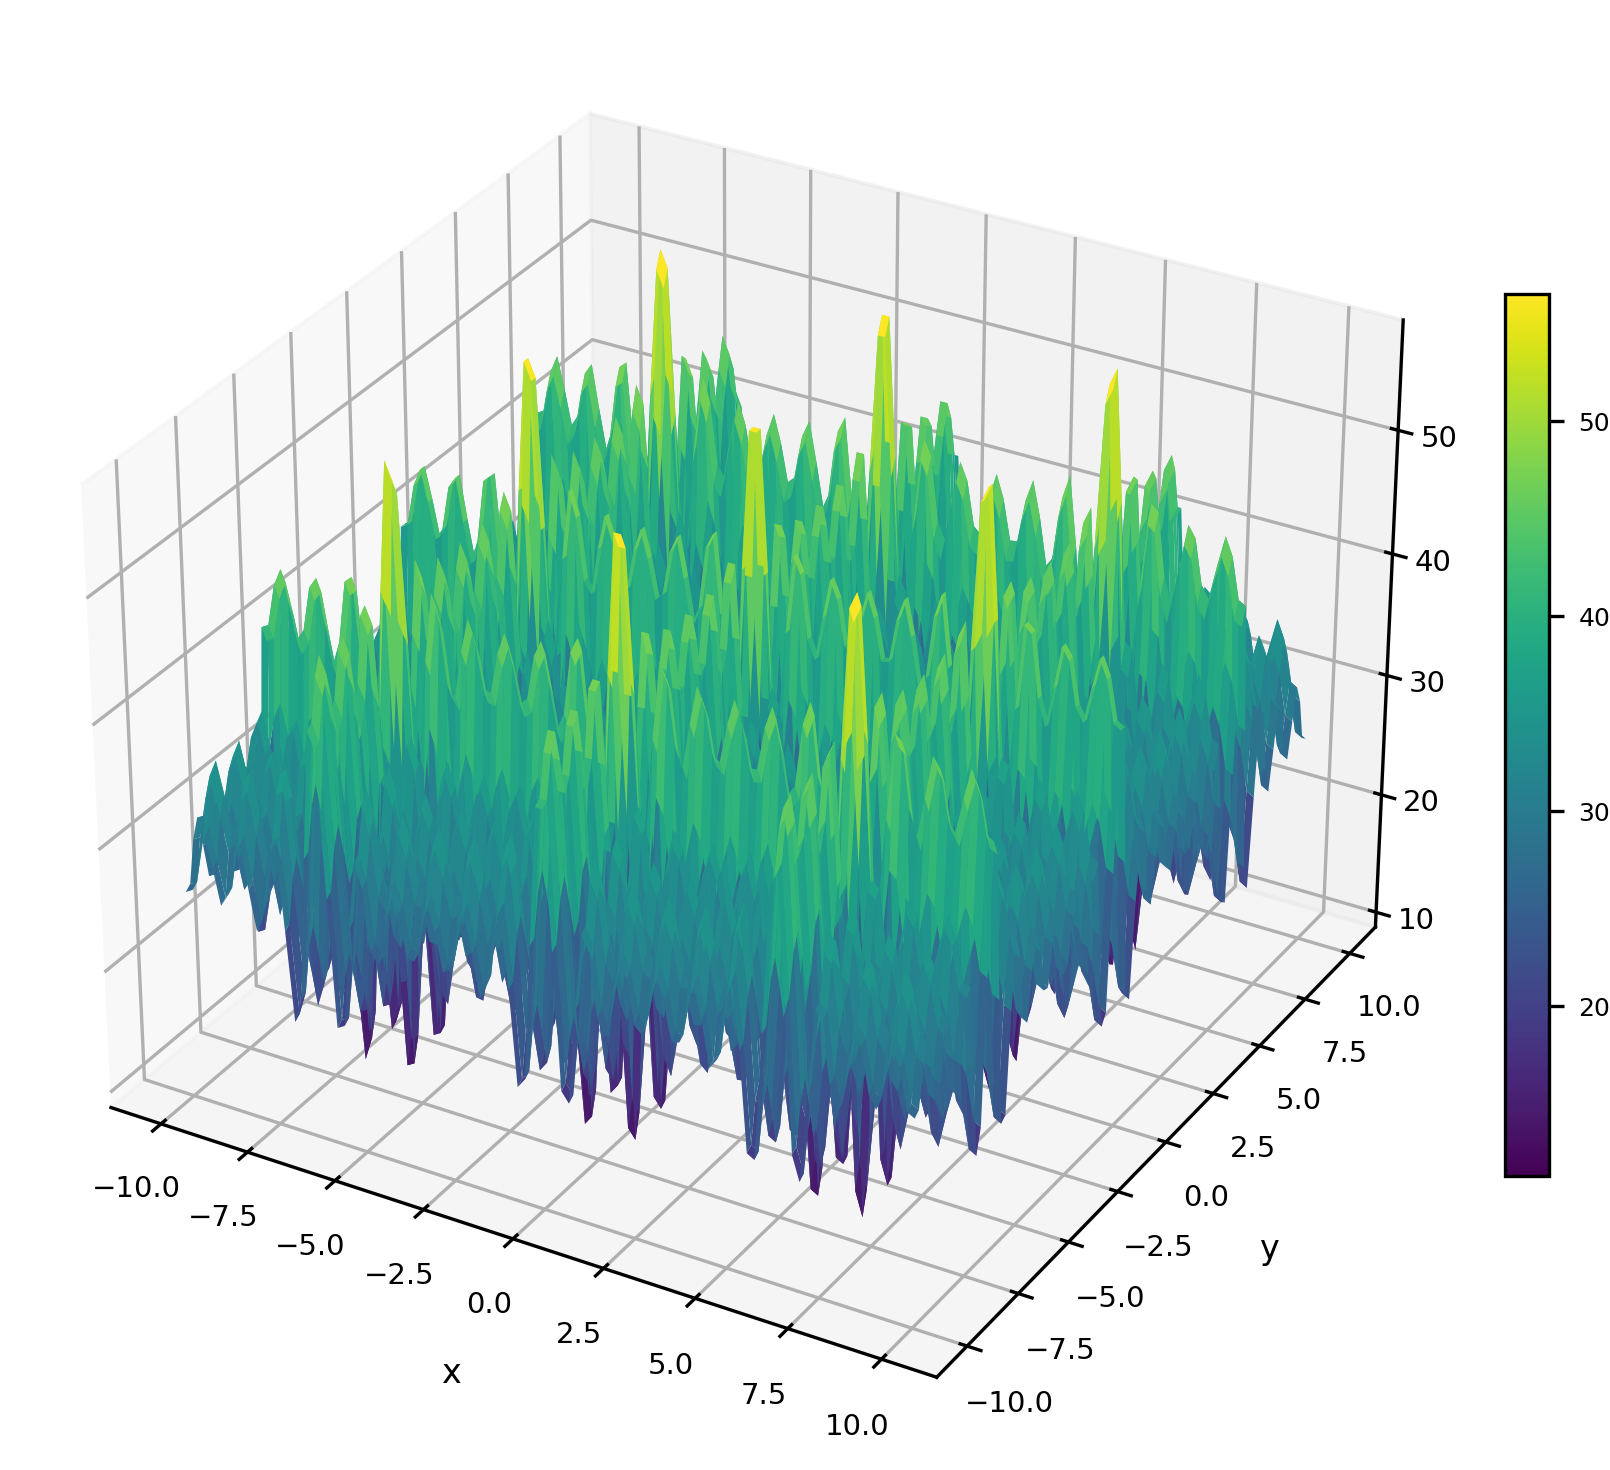
\includegraphics[width=1\textwidth]{Figures/benchmark_plots/Shubert_N4_maximized.png}
        \caption{Shubert N.4}
    \end{subfigure}
    % \hspace{.5cm} % Adjust the space as needed.
    \begin{subfigure}{0.32\textwidth}
        \centering
        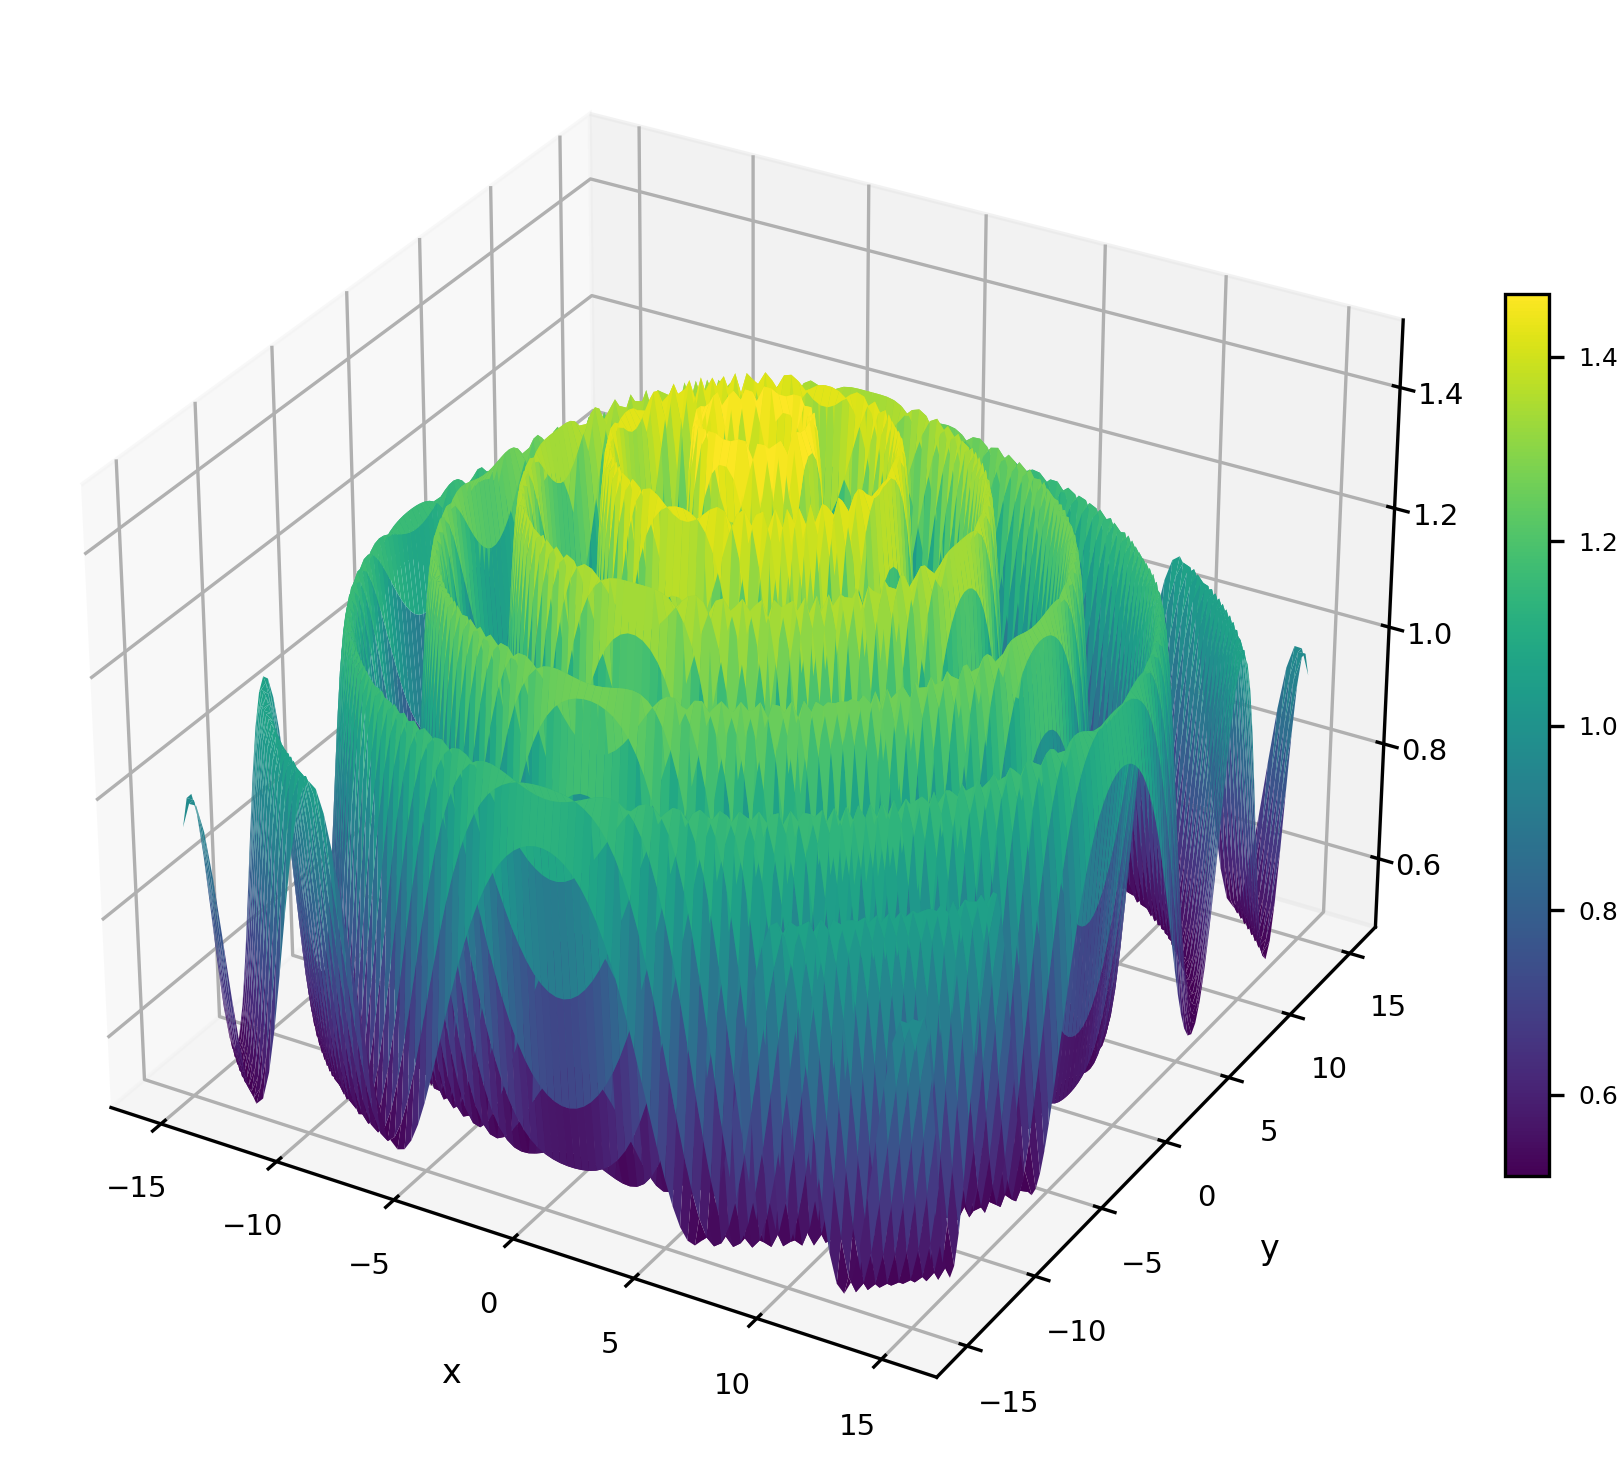
\includegraphics[width=1\textwidth]{Figures/benchmark_plots/SineEnvelope_maximized.png}
        \caption{Sine Envelope}
    \end{subfigure}
    \begin{subfigure}{0.32\textwidth}
        \centering
        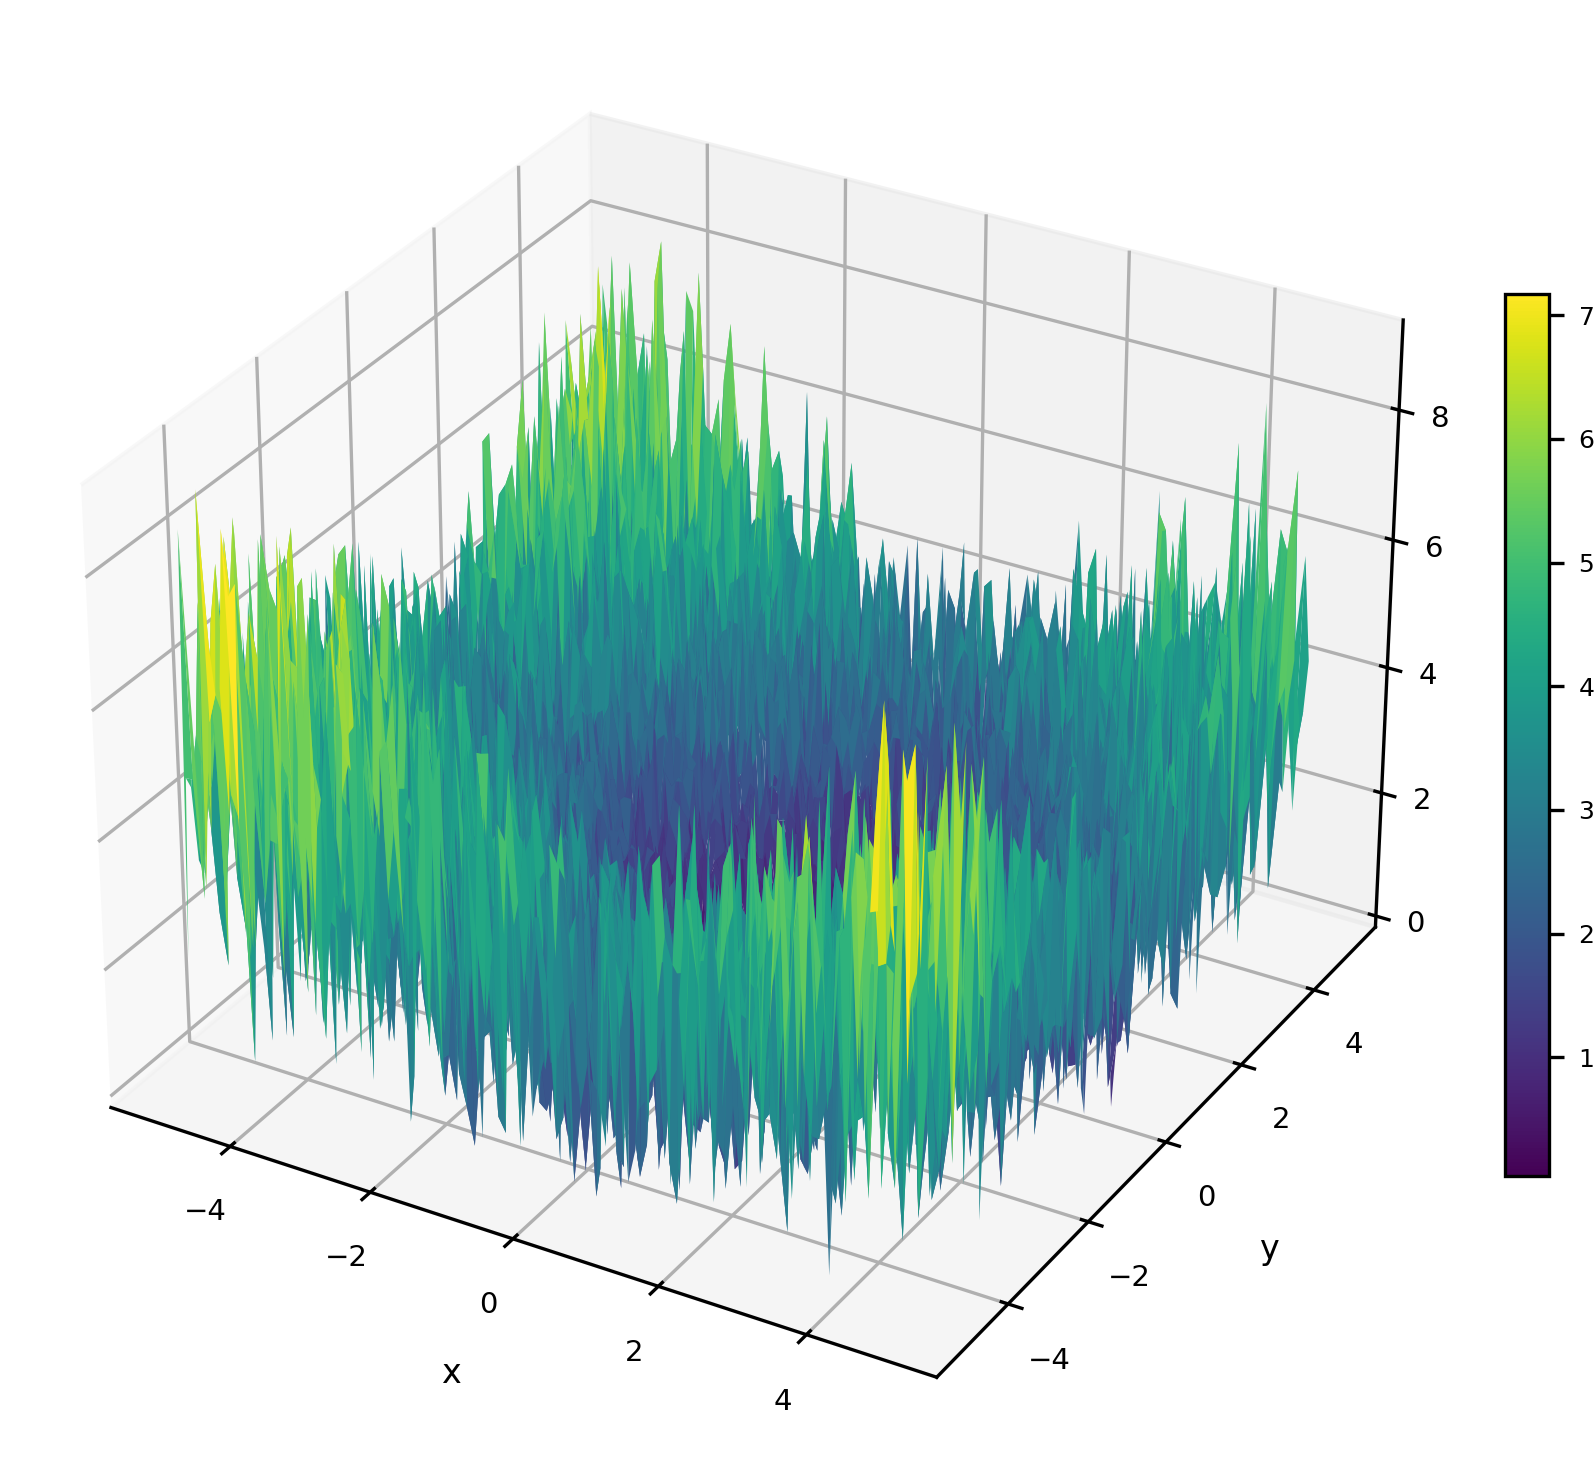
\includegraphics[width=1\textwidth]{Figures/benchmark_plots/Stochastic_maximized.png}
        \caption{Stochastic}
    \end{subfigure}
    % \hspace{.5cm} % Adjust the space as needed.
    \begin{subfigure}{0.32\textwidth}
        \centering
        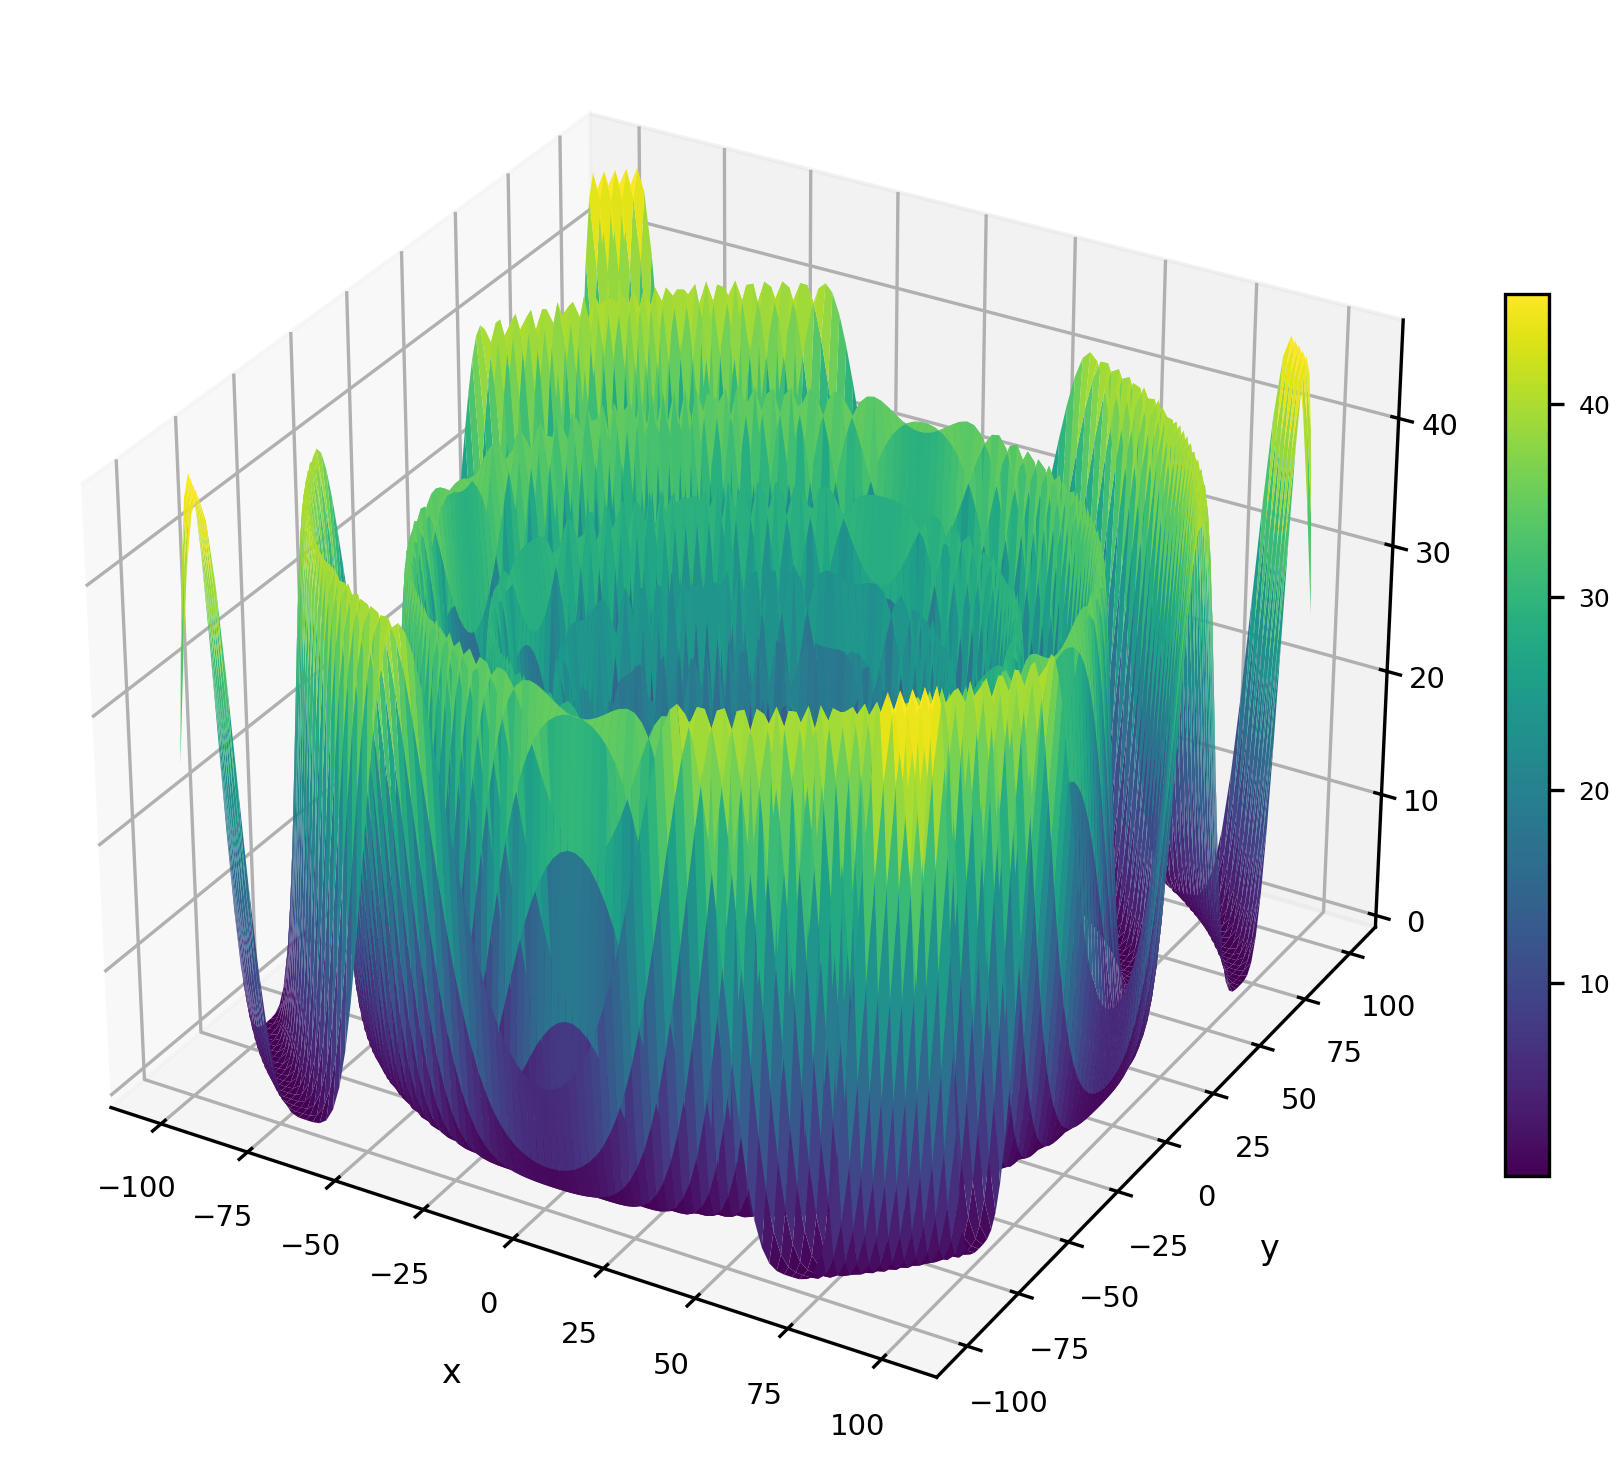
\includegraphics[width=1\textwidth]{Figures/benchmark_plots/StretchedV_maximized.png}
        \caption{Stretched V}
    \end{subfigure}
        \begin{subfigure}{0.32\textwidth}
        \centering
        \includegraphics[width=1\textwidth]{Figures/benchmark_plots/Styblinski–Tang_maximized.png}
        \caption{Styblinski–Tang}
    \end{subfigure}
        \captionsetup{list=no}
\caption{Two-dimensional visualizations of benchmark problem landscapes.}
\label{fig:benchmark_problems_plot}
\end{figure} % IMPORTANT!!!
\chapter{Parameter Optimization Results}\label{app:optimization results}

\enlargethispage{1\baselineskip}
\begin{longtable}{l
*{15}{>{\centering\arraybackslash}p{0.6cm}}
}
\caption[Parameter configurations]{Algorithm parameter configurations used in the experiments.}
\label{tab:parameter_configuration}\\
\toprule
\adjustbox{angle=90}{\textbf{Parameter}} &
\adjustbox{angle=90}{\textbf{PSO}} &
\adjustbox{angle=90}{\textbf{PerturbationPSO}} &
\adjustbox{angle=90}{\textbf{RebelPSO}} &
\adjustbox{angle=90}{\textbf{RejectorPSO}} &
\adjustbox{angle=90}{\textbf{RebelRejectorPSO}} &
\adjustbox{angle=90}{\textbf{ContrarianPSO}} &
\adjustbox{angle=90}{\textbf{DefeatistPSO}} &
\adjustbox{angle=90}{\textbf{ContrarianDefeatistPSO}} &
\adjustbox{angle=90}{\textbf{EschewerPSO}} &
\adjustbox{angle=90}{\textbf{EscapistPSO}} &
\adjustbox{angle=90}{\textbf{EschewerEscapistPSO}} &
\adjustbox{angle=90}{\textbf{HybridFullDisjointPSO}} &
\adjustbox{angle=90}{\textbf{HybridPartialDisjointPSO}} &
\adjustbox{angle=90}{\textbf{HybridAdditivePSO}} \\
\midrule
\endfirsthead

\toprule
\adjustbox{angle=90}{\textbf{Parameter}} &
\adjustbox{angle=90}{\textbf{PSO}} &
\adjustbox{angle=90}{\textbf{PerturbationPSO}} &
\adjustbox{angle=90}{\textbf{RebelPSO}} &
\adjustbox{angle=90}{\textbf{RejectorPSO}} &
\adjustbox{angle=90}{\textbf{RebelRejectorPSO}} &
\adjustbox{angle=90}{\textbf{ContrarianPSO}} &
\adjustbox{angle=90}{\textbf{DefeatistPSO}} &
\adjustbox{angle=90}{\textbf{ContrarianDefeatistPSO}} &
\adjustbox{angle=90}{\textbf{EschewerPSO}} &
\adjustbox{angle=90}{\textbf{EscapistPSO}} &
\adjustbox{angle=90}{\textbf{EschewerEscapistPSO}} &
\adjustbox{angle=90}{\textbf{HybridFullDisjointPSO}} &
\adjustbox{angle=90}{\textbf{HybridPartialDisjointPSO}} &
\adjustbox{angle=90}{\textbf{HybridAdditivePSO}} \\
\midrule
\endhead
$N$   & 100 & 100 & 100 & 100 & 100 & 100 & 100 & 100 & 100 & 100 & 100 & 100 & 100 & 100 \\
$\omega$   & 0.063 & 0.637 & 0.131 & 0.084 & 0.116 & 0.102 & 0.069 & 0.067 & 0.091 & 0.047 & 0.088 & 0.010 & 0.054 & 0.043 \\
$c_1$      & 4.373 & 2.545 & 0.308 & 1.545 & 1.292 & 0.405 & 0.405 & 0.905 & 2.177 & 2.577 & 0.900 & 2.519 & 5.251 & 0.254 \\
$c_2$      & 2.755 & 0.789 & 5.531 & 5.918 & 4.833 & 5.729 & 5.296 & 5.063 & 3.649 & 5.865 & 5.271 & 1.959 & 1.044 & 2.307 \\
$c_3$      & --    & --    & 3.923 & --    & 3.745 & --    & --    & --    & --    & --    & --    & 1.523 & 0.445 & 0.041 \\
$c_4$      & --    & --    & --    & 0.466 & 1.441 & --    & --    & --    & --    & --    & --    & 0.805 & 0.108 & 1.304 \\
$c_5$      & --    & --    & --    & --    & --    & 4.560 & --    & 4.333 & --    & --    & --    & 4.525 & 0.792 & 2.243 \\
$c_6$      & --    & --    & --    & --    & --    & --    & 0.953 & 1.746 & --    & --    & --    & 0.353 & 0.068 & 0.137 \\
$c_7$      & --    & --    & --    & --    & --    & --    & --    & --    & 1.658 & --    & 4.853 & 3.545 & 3.732 & 2.769 \\
$c_8$      & --    & --    & --    & --    & --    & --    & --    & --    & --    & 0.059 & 1.582 & 2.257 & 5.558 & 0.023 \\
$\sigma$   & --    & 0.008 & --    & --    & --    & --    & --    & --    & --    & --    & --    & --    & --    & --    \\
$\rho_1$   & --    & --    & --    & --    & --    & --    & --    & --    & --    & --    & --    & --    & --    & 0.880 \\
$\rho_2$   & --    & --    & --    & --    & --    & --    & --    & --    & --    & --    & --    & --    & --    & 0.764 \\
$\rho_3$   & --    & --    & 0.180 & --    & 0.189 & --    & --    & --    & --    & --    & --    & 0.071 & 0.114 & 0.476 \\
$\rho_4$   & --    & --    & --    & 0.679 & 0.194 & --    & --    & --    & --    & --    & --    & 0.353 & 0.393 & 0.536 \\
$\rho_5$   & --    & --    & --    & --    & --    & 0.480 & --    & 0.122 & --    & --    & --    & 0.035 & 0.365 & 0.460 \\
$\rho_6$   & --    & --    & --    & --    & --    & --    & 0.528 & 0.192 & --    & --    & --    & 0.388 & 0.570 & 0.539 \\
$\rho_7$   & --    & --    & --    & --    & --    & --    & --    & --    & 0.224 & --    & 0.163 & 0.136 & 0.172 & 0.315 \\
$\rho_8$   & --    & --    & --    & --    & --    & --    & --    & --    & --    & 0.476 & 0.230 & 0.016 & 0.038 & 0.463 \\
\bottomrule
\end{longtable}


\begin{figure}[H]
    \centering
    \begin{subfigure}{0.49\textwidth}
        \centering
        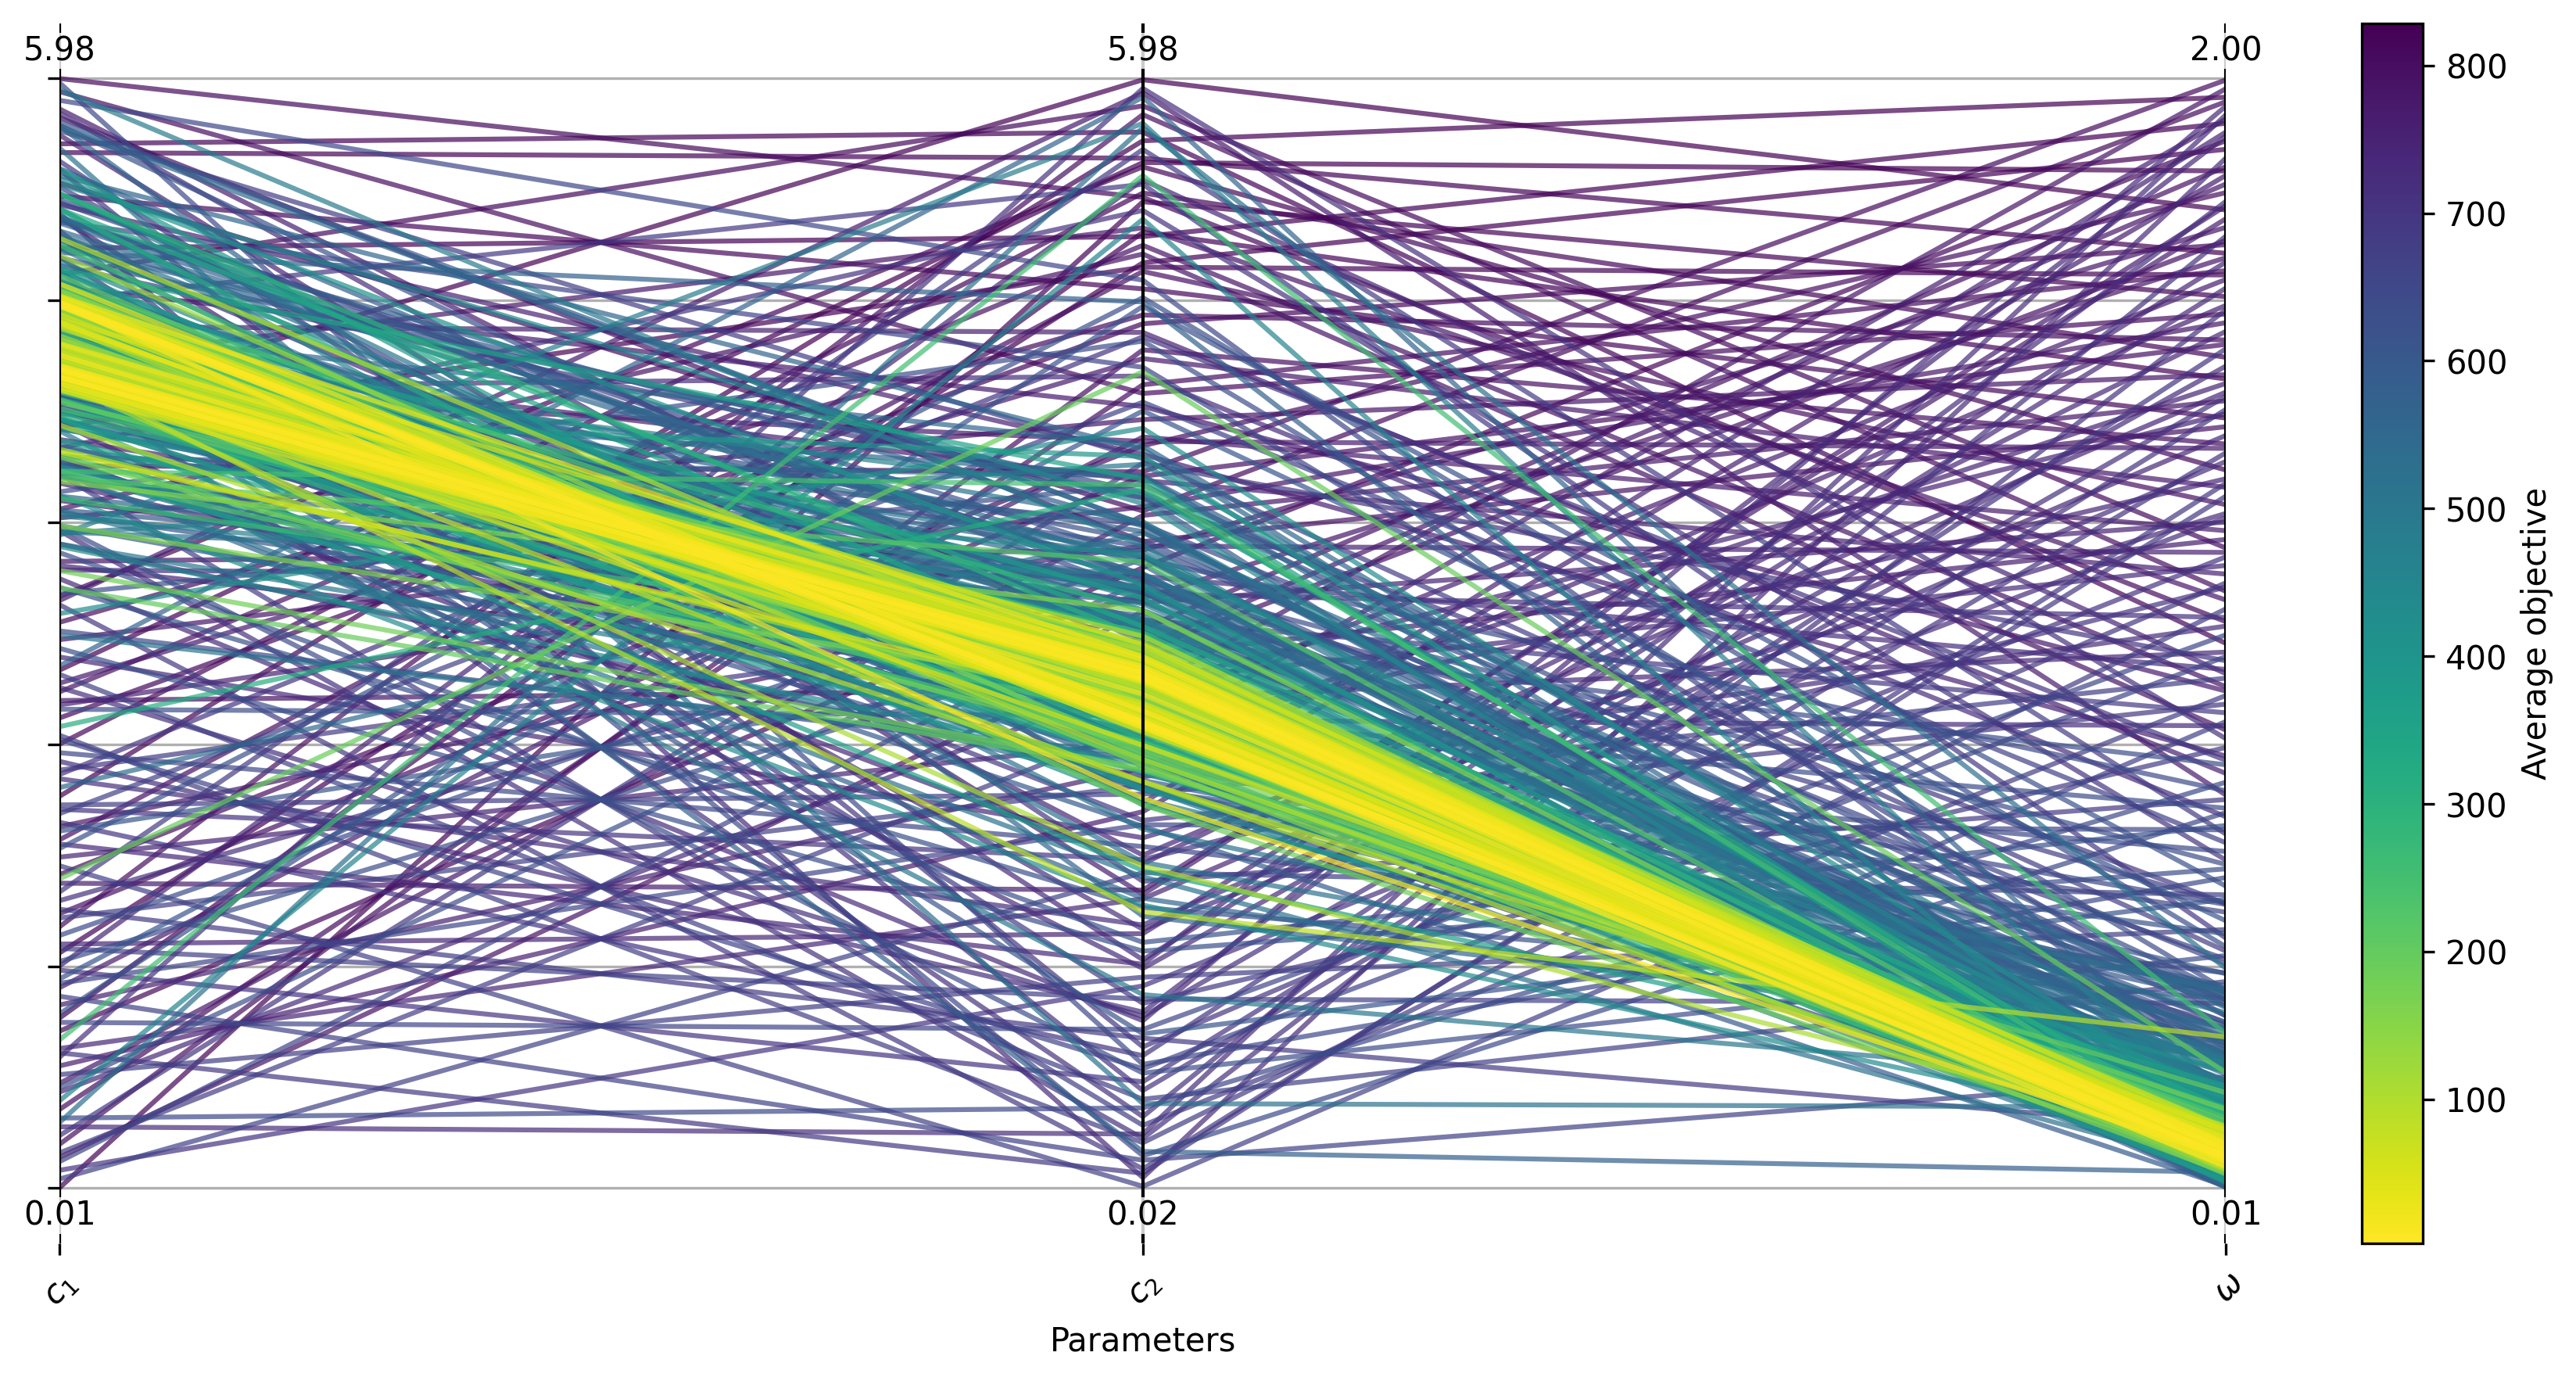
\includegraphics[width=1\textwidth]{Figures/tuning_plots/Parallel_coordinates_plot_for_PSO_parameters.png}
        \caption{PSO}
    \end{subfigure}
    % \hspace{.5cm} % Adjust the space as needed.
    \begin{subfigure}{0.49\textwidth}
        \centering
        \includegraphics[width=1\textwidth]{Figures/tuning_plots/Parallel_coordinates_plot_for_PerturbationPSO_parameters.png}
        \caption{PerturbationPSO}\label{fig:perturbation_params}
    \end{subfigure}
    \begin{subfigure}{0.49\textwidth}
        \centering
        \includegraphics[width=1\textwidth]{Figures/tuning_plots/Parallel_coordinates_plot_for_RebelPSO_parameters.png}
        \caption{RebelPSO}
    \end{subfigure}
    % \hspace{.5cm} % Adjust the space as needed.
    \begin{subfigure}{0.49\textwidth}
        \centering
        \includegraphics[width=1\textwidth]{Figures/tuning_plots/Parallel_coordinates_plot_for_RejectorPSO_parameters.png}
        \caption{RejectorPSO}
    \end{subfigure}
        \begin{subfigure}{0.49\textwidth}
        \centering
        \includegraphics[width=1\textwidth]{Figures/tuning_plots/Parallel_coordinates_plot_for_RebelRejectorPSO_parameters.png}
        \caption{RebelRejectorPSO}
    \end{subfigure}
        \begin{subfigure}{0.49\textwidth}
        \centering
        \includegraphics[width=1\textwidth]{Figures/tuning_plots/Parallel_coordinates_plot_for_ContrarianPSO_parameters.png}
        \caption{ContrarianPSO}
    \end{subfigure}
        \begin{subfigure}{0.49\textwidth}
        \centering
        \includegraphics[width=1\textwidth]{Figures/tuning_plots/Parallel_coordinates_plot_for_DefeatistPSO_parameters.png}
        \caption{DefeatistPSO}
    \end{subfigure}
      \begin{subfigure}{0.49\textwidth}
        \centering
        \includegraphics[width=1\textwidth]{Figures/tuning_plots/Parallel_coordinates_plot_for_ContrarianDefeatistPSO_parameters.png}
        \caption{ContrarianDefeatistPSO}
    \end{subfigure}
        \begin{subfigure}{0.49\textwidth}
        \centering
        \includegraphics[width=1\textwidth]{Figures/tuning_plots/Parallel_coordinates_plot_for_EschewerPSO_parameters.png}
        \caption{EschewerPSO}
    \end{subfigure}
    \begin{subfigure}{0.49\textwidth}
        \centering
        \includegraphics[width=1\textwidth]{Figures/tuning_plots/Parallel_coordinates_plot_for_EscapistPSO_parameters.png}
        \caption{EscapistPSO}
    \end{subfigure}
            \captionsetup{list=no}
\caption[Parallel coordinates plots of parameter configurations]{Parallel coordinates plots showing the distribution of  parameter configurations, colored by their average objective value.}
\end{figure}


\begin{figure}[H]\ContinuedFloat
    \centering
    \begin{subfigure}{0.49\textwidth}
        \centering
        \includegraphics[width=1\textwidth]{Figures/tuning_plots/Parallel_coordinates_plot_for_EschewerEscapistPSO_parameters.png}
        \caption{EschewerEscapistPSO}
    \end{subfigure}
    % \hspace{.5cm} % Adjust the space as needed.
    \begin{subfigure}{0.49\textwidth}
        \centering
        \includegraphics[width=1\textwidth]{Figures/tuning_plots/Parallel_coordinates_plot_for_HybridFullDisjointPSO_parameters.png}
        \caption{HybridFullDisjointPSO}
    \end{subfigure}
    \begin{subfigure}{0.49\textwidth}
        \centering
        \includegraphics[width=1\textwidth]{Figures/tuning_plots/Parallel_coordinates_plot_for_HybridPartialDisjointPSO_parameters.png}
        \caption{HybridPartialDisjointPSO}
    \end{subfigure}
    % \hspace{.5cm} % Adjust the space as needed.
    \begin{subfigure}{0.49\textwidth}
        \centering
        \includegraphics[width=1\textwidth]{Figures/tuning_plots/Parallel_coordinates_plot_for_HybridAdditivePSO_parameters.png}
        \caption{HybridAdditivePSO}
    \end{subfigure}
\caption[Parallel coordinates plots of parameter configurations]{Parallel coordinates plots showing the distribution of  parameter configurations, colored by their average objective value.}
\label{fig:parameter_plots}
\end{figure} % IMPORTANT!!!
\chapter{Detailed Results}\label{app:detailed_results}


This appendix provides the detailed results of the empirical experiments conducted in this study. Figure~\ref{fig:plot_encoding} illustrates the consistent line styles, color schemes, and numbering used for the convergence curves and final fitness distribution raincloud plots shown in Figures~\ref{fig:results100}, \ref{fig:results500}, and \ref{fig:results1000}. For clarity, nine plots displayed on a logarithmic scale are explicitly marked with “(log)” following the problem name.

\vfill

\vspace{.875em}
\begin{figure}[H]
\begin{tcbraster}[
    raster columns=2, 
    raster equal height, 
    nobeforeafter, 
    raster column skip=.1cm
]
\begin{colorblock}{Baseline}{note}
\begin{scriptsize}
\textbf{1}. PSO \quad \rule[0.5ex]{2em}{0.35pt} \colorbox{kit-gray100}{\color{white}\textbf{black}}\\
\textbf{2}. PerturbationPSO \quad $- - -$  \colorbox{kit-gray50}{\color{white}\textbf{gray}}\end{scriptsize}
\end{colorblock}
\begin{colorblock}{Repulsion strategy}{tip}
\begin{scriptsize}
\textbf{3}. RebelPSO \quad $\mathbf{- \cdot -\, \cdot }$ \colorbox{tiplight}{\textbf{light green}} \\
\textbf{4}. RejectorPSO \quad $\mathbf{\cdots\cdots }$ \colorbox{tipmedium}{\textbf{medium green}} \\
\textbf{5}. RebelRejectorPSO \quad $\mathbf{- \cdot \cdot - \cdot}$ \colorbox{tipdark}{\textbf{dark green}} \end{scriptsize}
\end{colorblock}
\end{tcbraster}

\begin{tcbraster}[
    raster columns=2, 
    raster equal height, 
    nobeforeafter, 
    raster column skip=.1cm
]
\begin{colorblock}{Negative learning strategies}{warning}
\begin{scriptsize}
\textbf{6}. ContrarianPSO \quad \rule[0.5ex]{2em}{0.35pt} \colorbox{warninglight}{\textbf{light yellow}} \\
\textbf{7}. DefeatistPSO \quad $- - -$ \colorbox{warningpale}{\textbf{medium yellow}}\\
\textbf{8}. ContrarianDefeatistPSO \quad $\mathbf{- \cdot -\, \cdot }$ \colorbox{warningmedium}{\textbf{dark yellow}}\end{scriptsize}
\end{colorblock}
\begin{colorblock}{Reverse learning strategies}{infodarkest}
\begin{scriptsize}
\textbf{9}. EschewerPSO \quad $\mathbf{\cdots\cdots }$ \colorbox{infolight}{\textbf{light blue}} \\
\textbf{10}. EscapistPSO \quad$\mathbf{- \cdot \cdot - \cdot}$  \colorbox{infomediumpale}{\textbf{medium blue}}\\
\textbf{11}. EschewerEscapistPSO \quad  \rule[0.5ex]{2em}{0.35pt} \colorbox{infodarklight}{\textbf{dark blue}}\end{scriptsize}
\end{colorblock}
\end{tcbraster}

\begin{colorblock}{Multi-hybrid strategies}{todo}
\begin{scriptsize}
\textbf{12}. HybridFullDisjointPSO \quad $- - -$ \colorbox{todolight}{\textbf{light red}} \\
\textbf{13}. HybridPartialDisjointPSO \quad $\mathbf{- \cdot -\, \cdot }$ \colorbox{todomedium}{\textbf{medium red}}\\
\textbf{14}. HybridAdditivePSO \quad $\mathbf{\cdots\cdots }$ \colorbox{tododark}{\textbf{dark red}}\end{scriptsize}
\end{colorblock}
\caption[Plots encoding]{Numbering, line styles, and color coding used consistently for the convergence and final fitness distribution plots throughout this appendix.}
    \label{fig:plot_encoding}
\end{figure}
\vspace{.875em}







% \newpage


\begin{figure}[p]
\renewcommand\thesubfigure{C.\arabic{figure}.\arabic{subfigure}} % Local change starts here

    \centering
\begin{subfigure}{1\textwidth}
    \centering
    \includegraphics[width=.49\textwidth]{Figures/results/100/Alpine_N1_All_selected_algorithms_dim100_annot_legend.png}
    \includegraphics[width=.49\textwidth]{Figures/results/100/Alpine_N1_all_dim100_raincloud_vertical.png}
    \caption{Alpine N.1 (log)}
\end{subfigure}

\begin{subfigure}{1\textwidth}
    \centering
    \includegraphics[width=.49\textwidth]{Figures/results/100/Crowned_Cross_All_selected_algorithms_dim100_annot_legend.png}
    \includegraphics[width=.49\textwidth]{Figures/results/100/Crowned_Cross_all_dim100_raincloud_vertical.png}
    \caption{Crowned Cross}
\end{subfigure}

\begin{subfigure}{1\textwidth}
    \centering
    \includegraphics[width=.49\textwidth]{Figures/results/100/Egg_Holder_All_selected_algorithms_dim100_annot_legend.png}
    \includegraphics[width=.49\textwidth]{Figures/results/100/Egg_Holder_all_dim100_raincloud_vertical.png}
    \caption{Egg-Holder}
\end{subfigure}

\begin{subfigure}{1\textwidth}
    \centering
    \includegraphics[width=.49\textwidth]{Figures/results/100/Expanded_Shaffer_All_selected_algorithms_dim100_annot_legend.png}
    \includegraphics[width=.49\textwidth]{Figures/results/100/Expanded_Shaffer_all_dim100_raincloud_vertical.png}
    \caption{Expanded Shaffer}
\end{subfigure}

\begin{subfigure}{1\textwidth}
    \centering
    \includegraphics[width=.49\textwidth]{Figures/results/100/Generalized_Schaffer_N1_All_selected_algorithms_dim100_annot_legend.png}
    \includegraphics[width=.49\textwidth]{Figures/results/100/Generalized_Schaffer_N1_all_dim100_raincloud_vertical.png}
    \caption{Generalized Schaffer N.1}
\end{subfigure}

\begin{subfigure}{1\textwidth}
    \centering
    \includegraphics[width=.49\textwidth]{Figures/results/100/Generalized_Schaffer_N2_All_selected_algorithms_dim100_annot_legend.png}
    \includegraphics[width=.49\textwidth]{Figures/results/100/Generalized_Schaffer_N2_all_dim100_raincloud_vertical.png}
    \caption{Generalized Schaffer N.2}
\end{subfigure}

% \enlargethispage{3\baselineskip}
            \captionsetup{list=no}
\caption[Convergence curves and final fitness distribution raincloud plots for 100-dimensional problems]{Convergence curves (left) and final fitness distribution raincloud plots (right) for each tested benchmark problem in the 100-dimensional setting. Algorithms are numbered, line-styled, ordered, and color-coded consistently according to the legend in Figure~\ref{fig:plot_encoding}. Problems plotted on a logarithmic scale are indicated with ``(log)'' following the problem name.}

\end{figure}




%%%%%%%%%%%%%%%%%%%%%%%%%%%




\begin{figure}[p]\ContinuedFloat
\renewcommand\thesubfigure{C.\arabic{figure}.\arabic{subfigure}} % Local change starts here

    \centering

\begin{subfigure}{1\textwidth}
    \centering
    \includegraphics[width=.49\textwidth]{Figures/results/100/Generalized_Schaffer_N3_All_selected_algorithms_dim100_annot_legend.png}
    \includegraphics[width=.49\textwidth]{Figures/results/100/Generalized_Schaffer_N3_all_dim100_raincloud_vertical.png}
    \caption{Generalized Schaffer N3}
\end{subfigure}

\begin{subfigure}{1\textwidth}
    \centering
    \includegraphics[width=.49\textwidth]{Figures/results/100/Generalized_Schaffer_N4_All_selected_algorithms_dim100_annot_legend.png}
    \includegraphics[width=.49\textwidth]{Figures/results/100/Generalized_Schaffer_N4_all_dim100_raincloud_vertical.png}
    \caption{Generalized Schaffer N4}
\end{subfigure}

\begin{subfigure}{1\textwidth}
    \centering
    \includegraphics[width=.49\textwidth]{Figures/results/100/Generalized_Schmidt–Vetters_All_selected_algorithms_dim100_annot_legend.png}
    \includegraphics[width=.49\textwidth]{Figures/results/100/Generalized_Schmidt–Vetters_all_dim100_raincloud_vertical.png}
    \caption{Generalized Schmidt–Vetters}
\end{subfigure}

\begin{subfigure}{1\textwidth}
    \centering
    \includegraphics[width=.49\textwidth]{Figures/results/100/Lennard_Jones_Minimum_Energy_Cluster_All_selected_algorithms_dim100_annot_legend.png}
    \includegraphics[width=.49\textwidth]{Figures/results/100/Lennard_Jones_Minimum_Energy_Cluster_all_dim100_raincloud_vertical.png}
    \caption{Lennard-Jones Minimum Energy Cluster}
\end{subfigure}

\begin{subfigure}{1\textwidth}
    \centering
    \includegraphics[width=.49\textwidth]{Figures/results/100/Michalewicz_All_selected_algorithms_dim100_annot_legend.png}
    \includegraphics[width=.49\textwidth]{Figures/results/100/Michalewicz_all_dim100_raincloud_vertical.png}
    \caption{Michalewicz}
\end{subfigure}

\begin{subfigure}{1\textwidth}
    \centering
    \includegraphics[width=.49\textwidth]{Figures/results/100/Mishra_N3_All_selected_algorithms_dim100_annot_legend.png}
    \includegraphics[width=.49\textwidth]{Figures/results/100/Mishra_N3_all_dim100_raincloud_vertical.png}
    \caption{Mishra N3}
\end{subfigure}


\captionsetup{list=no}
\caption[Convergence curves and final fitness distribution raincloud plots for 100-dimensional problems]{Convergence curves (left) and final fitness distribution raincloud plots (right) for each tested benchmark problem in the 100-dimensional setting. Algorithms are numbered, line-styled, ordered, and color-coded consistently according to the legend in Figure~\ref{fig:plot_encoding}. Problems plotted on a logarithmic scale are indicated with ``(log)'' following the problem name.}
\end{figure}




%%%%%%%%%%%%%%%%%%%%%%%%%%%



\begin{figure}[p]\ContinuedFloat
\renewcommand\thesubfigure{C.\arabic{figure}.\arabic{subfigure}} % Local change starts here

    \centering

\begin{subfigure}{1\textwidth}
    \centering
    \includegraphics[width=.49\textwidth]{Figures/results/100/Mishra_N4_All_selected_algorithms_dim100_annot_legend.png}
    \includegraphics[width=.49\textwidth]{Figures/results/100/Mishra_N4_all_dim100_raincloud_vertical.png}
    \caption{Mishra N4}
\end{subfigure}

\begin{subfigure}{1\textwidth}
    \centering
    \includegraphics[width=.49\textwidth]{Figures/results/100/Modified_Rosenbrock_No.02___Hollow_Ground_Bent_Knife_Edge_All_selected_algorithms_dim100_annot_legend.png}
    \includegraphics[width=.49\textwidth]{Figures/results/100/Modified_Rosenbrock_No.02___Hollow_Ground_Bent_Knife_Edge_all_dim100_raincloud_vertical.png}
    \caption{Modified Rosenbrock N.2 (log)}
\end{subfigure}

\begin{subfigure}{1\textwidth}
    \centering
    \includegraphics[width=.49\textwidth]{Figures/results/100/Rotated_Bent_Cigar_All_selected_algorithms_dim100_annot_legend.png}
    \includegraphics[width=.49\textwidth]{Figures/results/100/Rotated_Bent_Cigar_all_dim100_raincloud_vertical.png}
    \caption{Rotated Bent Cigar (log)}
\end{subfigure}

\begin{subfigure}{1\textwidth}
    \centering
    \includegraphics[width=.49\textwidth]{Figures/results/100/Rotated_Discus_All_selected_algorithms_dim100_annot_legend.png}
    \includegraphics[width=.49\textwidth]{Figures/results/100/Rotated_Discus_all_dim100_raincloud_vertical.png}
    \caption{Rotated Discus (log)}
\end{subfigure}

\begin{subfigure}{1\textwidth}
    \centering
    \includegraphics[width=.49\textwidth]{Figures/results/100/Rotated_High_Conditioned_Elliptic_All_selected_algorithms_dim100_annot_legend.png}
    \includegraphics[width=.49\textwidth]{Figures/results/100/Rotated_High_Conditioned_Elliptic_all_dim100_raincloud_vertical.png}
    \caption{Rotated High Conditioned Elliptic (log)}
\end{subfigure}

\begin{subfigure}{1\textwidth}
    \centering
    \includegraphics[width=.49\textwidth]{Figures/results/100/Salomon_All_selected_algorithms_dim100_annot_legend.png}
    \includegraphics[width=.49\textwidth]{Figures/results/100/Salomon_all_dim100_raincloud_vertical.png}
    \caption{Salomon (log)}
\end{subfigure}

    \captionsetup{list=no}
\caption[Convergence curves and final fitness distribution raincloud plots for 100-dimensional problems]{Convergence curves (left) and final fitness distribution raincloud plots (right) for each tested benchmark problem in the 100-dimensional setting. Algorithms are numbered, line-styled, ordered, and color-coded consistently according to the legend in Figure~\ref{fig:plot_encoding}. Problems plotted on a logarithmic scale are indicated with ``(log)'' following the problem name.}
\end{figure}


%%%%%%%%%


\begin{figure}[p]\ContinuedFloat
\renewcommand\thesubfigure{C.\arabic{figure}.\arabic{subfigure}} % Local change starts here

    \centering

\begin{subfigure}{1\textwidth}
    \centering
    \includegraphics[width=.49\textwidth]{Figures/results/100/Schwefel_N20_All_selected_algorithms_dim100_annot_legend.png}
    \includegraphics[width=.49\textwidth]{Figures/results/100/Schwefel_N20_all_dim100_raincloud_vertical.png}
    \caption{Schwefel N.20}
\end{subfigure}

\begin{subfigure}{1\textwidth}
    \centering
    \includegraphics[width=.49\textwidth]{Figures/results/100/Schwefel_N36_All_selected_algorithms_dim100_annot_legend.png}
    \includegraphics[width=.49\textwidth]{Figures/results/100/Schwefel_N36_all_dim100_raincloud_vertical.png}
    \caption{Schwefel N36}
\end{subfigure}

\begin{subfigure}{1\textwidth}
    \centering
    \includegraphics[width=.49\textwidth]{Figures/results/100/Schwefel_N6_All_selected_algorithms_dim100_annot_legend.png}
    \includegraphics[width=.49\textwidth]{Figures/results/100/Schwefel_N6_all_dim100_raincloud_vertical.png}
    \caption{Schwefel N6 (log)}
\end{subfigure}

\begin{subfigure}{1\textwidth}
    \centering
    \includegraphics[width=.49\textwidth]{Figures/results/100/Shifted_Schwefel_All_selected_algorithms_dim100_annot_legend.png}
    \includegraphics[width=.49\textwidth]{Figures/results/100/Shifted_Schwefel_all_dim100_raincloud_vertical.png}
    \caption{Shifted Schwefel}
\end{subfigure}

\begin{subfigure}{1\textwidth}
    \centering
    \includegraphics[width=.49\textwidth]{Figures/results/100/Shifted_and_Rotated_HGBat_All_selected_algorithms_dim100_annot_legend.png}
    \includegraphics[width=.49\textwidth]{Figures/results/100/Shifted_and_Rotated_HGBat_all_dim100_raincloud_vertical.png}
    \caption{Shifted and Rotated HGBat}
\end{subfigure}

\begin{subfigure}{1\textwidth}
    \centering
    \includegraphics[width=.49\textwidth]{Figures/results/100/Shifted_and_Rotated_HappyCat_All_selected_algorithms_dim100_annot_legend.png}
    \includegraphics[width=.49\textwidth]{Figures/results/100/Shifted_and_Rotated_HappyCat_all_dim100_raincloud_vertical.png}
    \caption{Shifted and Rotated HappyCat}
\end{subfigure}

\enlargethispage{1\baselineskip}
\captionsetup{list=no}
\caption[Convergence curves and final fitness distribution raincloud plots for 100-dimensional problems]{Convergence curves (left) and final fitness distribution raincloud plots (right) for each tested benchmark problem in the 100-dimensional setting. Algorithms are numbered, line-styled, ordered, and color-coded consistently according to the legend in Figure~\ref{fig:plot_encoding}. Problems plotted on a logarithmic scale are indicated with ``(log)'' following the problem name.}
\end{figure}


% %%%%%%%%%


\begin{figure}[p]\ContinuedFloat
\renewcommand\thesubfigure{C.\arabic{figure}.\arabic{subfigure}} % Local change starts here

    \centering

\begin{subfigure}{1\textwidth}
    \centering
    \includegraphics[width=.49\textwidth]{Figures/results/100/Shifted_and_Rotated_Expanded_Scaffer’s_F6_All_selected_algorithms_dim100_annot_legend.png}
    \includegraphics[width=.49\textwidth]{Figures/results/100/Shifted_and_Rotated_Expanded_Scaffer’s_F6_all_dim100_raincloud_vertical.png}
    \caption{Shifted and Rotated Schaffer F7}
\end{subfigure}

\begin{subfigure}{1\textwidth}
    \centering
    \includegraphics[width=.49\textwidth]{Figures/results/100/Shifted_and_Rotated_Weierstrass_All_selected_algorithms_dim100_annot_legend.png}
    \includegraphics[width=.49\textwidth]{Figures/results/100/Shifted_and_Rotated_Weierstrass_all_dim100_raincloud_vertical.png}
    \caption{Shifted and Rotated Weierstrass}
\end{subfigure}

\begin{subfigure}{1\textwidth}
    \centering
    \includegraphics[width=.49\textwidth]{Figures/results/100/Shubert_N3_All_selected_algorithms_dim100_annot_legend.png}
    \includegraphics[width=.49\textwidth]{Figures/results/100/Shubert_N3_all_dim100_raincloud_vertical.png}
    \caption{Shubert N3}
\end{subfigure}

\begin{subfigure}{1\textwidth}
    \centering
    \includegraphics[width=.49\textwidth]{Figures/results/100/Shubert_N4_All_selected_algorithms_dim100_annot_legend.png}
    \includegraphics[width=.49\textwidth]{Figures/results/100/Shubert_N4_all_dim100_raincloud_vertical.png}
    \caption{Shubert N4}
\end{subfigure}

\begin{subfigure}{1\textwidth}
    \centering
    \includegraphics[width=.49\textwidth]{Figures/results/100/SineEnvelope_All_selected_algorithms_dim100_annot_legend.png}
    \includegraphics[width=.49\textwidth]{Figures/results/100/SineEnvelope_all_dim100_raincloud_vertical.png}
    \caption{Sine Envelope}
\end{subfigure}

\begin{subfigure}{1\textwidth}
    \centering
    \includegraphics[width=.49\textwidth]{Figures/results/100/Stochastic_All_selected_algorithms_dim100_annot_legend.png}
    \includegraphics[width=.49\textwidth]{Figures/results/100/Stochastic_all_dim100_raincloud_vertical.png}
    \caption{Stochastic (log)}
\end{subfigure}

\captionsetup{list=no}
\caption[Convergence curves and final fitness distribution raincloud plots for 100-dimensional problems]{Convergence curves (left) and final fitness distribution raincloud plots (right) for each tested benchmark problem in the 100-dimensional setting. Algorithms are numbered, line-styled, ordered, and color-coded consistently according to the legend in Figure~\ref{fig:plot_encoding}. Problems plotted on a logarithmic scale are indicated with ``(log)'' following the problem name.}
\end{figure}



% %%%%%%%%%


\begin{figure}[H]\ContinuedFloat
\renewcommand\thesubfigure{C.\arabic{figure}.\arabic{subfigure}} % Local change starts here

    \centering

\begin{subfigure}{1\textwidth}
    \centering
    \includegraphics[width=.49\textwidth]{Figures/results/100/StretchedV_All_selected_algorithms_dim100_annot_legend.png}
    \includegraphics[width=.49\textwidth]{Figures/results/100/StretchedV_all_dim100_raincloud_vertical.png}
    \caption{StretchedV (log)}
\end{subfigure}

\begin{subfigure}{1\textwidth}
    \centering
    \includegraphics[width=.49\textwidth]{Figures/results/100/Styblinski–Tang_All_selected_algorithms_dim100_annot_legend.png}
    \includegraphics[width=.49\textwidth]{Figures/results/100/Styblinski–Tang_all_dim100_raincloud_vertical.png}
    \caption{Styblinski–Tang}
\end{subfigure}

\caption[Convergence curves and final fitness distribution raincloud plots for\\100-dimensional problems]{Convergence curves (left) and final fitness distribution raincloud plots (right) for each tested benchmark problem in the 100-dimensional setting. Algorithms are numbered, line-styled, ordered, and color-coded consistently according to the legend in Figure~\ref{fig:plot_encoding}. Problems plotted on a logarithmic scale are indicated with ``(log)'' following the problem name.}
\label{fig:results100}
\end{figure}


% %%%%%%%%%
%%%%%%%%%%%%%%%%%%%%%%%%%%%%%%%%%%%%%%%%%%%%%%%%%%%%%%%%%%%%%%%%%%%%%%%%%%%%
%%%%%%%%%%%%%%%%%%%%%%%%%%%%%%%%%%%%%%%%%%%%%%%%%%%%%%%%%%%%%%%%%%%%%%%%%%%%
%%%%%%%%%%%%%%%%%%%%%%%%%%%%%%%%%%%%%%%%%%%%%%%%%%%%%%%%%%%%%%%%%%%%%%%%%%%%



\vfill
% \vspace{.875em}


\begin{figure}[H]
\renewcommand\thesubfigure{C.\arabic{figure}.\arabic{subfigure}} % Local change starts here

    \centering

    \begin{subfigure}{1\textwidth}
    \centering
    \includegraphics[width=.49\textwidth]{Figures/results/500/Alpine_N1_All_selected_algorithms_dim500_annot_legend.png}
    \includegraphics[width=.49\textwidth]{Figures/results/500/Alpine_N1_all_dim500_raincloud_vertical.png}
    \caption{Alpine N.1 (log)}
\end{subfigure}

\begin{subfigure}{1\textwidth}
    \centering
    \includegraphics[width=.49\textwidth]{Figures/results/500/Crowned_Cross_All_selected_algorithms_dim500_annot_legend.png}
    \includegraphics[width=.49\textwidth]{Figures/results/500/Crowned_Cross_all_dim500_raincloud_vertical.png}
    \caption{Crowned Cross}
\end{subfigure}

\begin{subfigure}{1\textwidth}
    \centering
    \includegraphics[width=.49\textwidth]{Figures/results/500/Egg_Holder_All_selected_algorithms_dim500_annot_legend.png}
    \includegraphics[width=.49\textwidth]{Figures/results/500/Egg_Holder_all_dim500_raincloud_vertical.png}
    \caption{Egg-Holder}
\end{subfigure}

\captionsetup{list=no}
\caption[Convergence curves and final fitness distribution raincloud plots for\\500-dimensional problems]{Convergence curves (left) and final fitness distribution raincloud plots (right) for each tested benchmark problem in the 500-dimensional setting. Algorithms are numbered, line-styled, ordered, and color-coded consistently according to the legend in Figure~\ref{fig:plot_encoding}. Problems plotted on a logarithmic scale are indicated with ``(log)'' following the problem name.}
\end{figure}



% %%%%%%%%%


\begin{figure}[p]\ContinuedFloat
\renewcommand\thesubfigure{C.\arabic{figure}.\arabic{subfigure}} % Local change starts here

    \centering

\begin{subfigure}{1\textwidth}
    \centering
    \includegraphics[width=.49\textwidth]{Figures/results/500/Expanded_Shaffer_All_selected_algorithms_dim500_annot_legend.png}
    \includegraphics[width=.49\textwidth]{Figures/results/500/Expanded_Shaffer_all_dim500_raincloud_vertical.png}
    \caption{Expanded Shaffer}
\end{subfigure}

\begin{subfigure}{1\textwidth}
    \centering
    \includegraphics[width=.49\textwidth]{Figures/results/500/Generalized_Schaffer_N1_All_selected_algorithms_dim500_annot_legend.png}
    \includegraphics[width=.49\textwidth]{Figures/results/500/Generalized_Schaffer_N1_all_dim500_raincloud_vertical.png}
    \caption{Generalized Schaffer N.1}
\end{subfigure}

\begin{subfigure}{1\textwidth}
    \centering
    \includegraphics[width=.49\textwidth]{Figures/results/500/Generalized_Schaffer_N2_All_selected_algorithms_dim500_annot_legend.png}
    \includegraphics[width=.49\textwidth]{Figures/results/500/Generalized_Schaffer_N2_all_dim500_raincloud_vertical.png}
    \caption{Generalized Schaffer N.2}
\end{subfigure}

\begin{subfigure}{1\textwidth}
    \centering
    \includegraphics[width=.49\textwidth]{Figures/results/500/Generalized_Schaffer_N3_All_selected_algorithms_dim500_annot_legend.png}
    \includegraphics[width=.49\textwidth]{Figures/results/500/Generalized_Schaffer_N3_all_dim500_raincloud_vertical.png}
    \caption{Generalized Schaffer N3}
\end{subfigure}

\begin{subfigure}{1\textwidth}
    \centering
    \includegraphics[width=.49\textwidth]{Figures/results/500/Generalized_Schaffer_N4_All_selected_algorithms_dim500_annot_legend.png}
    \includegraphics[width=.49\textwidth]{Figures/results/500/Generalized_Schaffer_N4_all_dim500_raincloud_vertical.png}
    \caption{Generalized Schaffer N4}
\end{subfigure}

\begin{subfigure}{1\textwidth}
    \centering
    \includegraphics[width=.49\textwidth]{Figures/results/500/Generalized_Schmidt–Vetters_All_selected_algorithms_dim500_annot_legend.png}
    \includegraphics[width=.49\textwidth]{Figures/results/500/Generalized_Schmidt–Vetters_all_dim500_raincloud_vertical.png}
    \caption{Generalized Schmidt–Vetters}
\end{subfigure}

\captionsetup{list=no}
\caption[Convergence curves and final fitness distribution raincloud plots for 500-dimensional problems]{Convergence curves (left) and final fitness distribution raincloud plots (right) for each tested benchmark problem in the 500-dimensional setting. Algorithms are numbered, line-styled, ordered, and color-coded consistently according to the legend in Figure~\ref{fig:plot_encoding}. Problems plotted on a logarithmic scale are indicated with ``(log)'' following the problem name.}
\end{figure}



% %%%%%%%%%


\begin{figure}[p]\ContinuedFloat
\renewcommand\thesubfigure{C.\arabic{figure}.\arabic{subfigure}} % Local change starts here

    \centering

\begin{subfigure}{1\textwidth}
    \centering
    \includegraphics[width=.49\textwidth]{Figures/results/500/Lennard_Jones_Minimum_Energy_Cluster_All_selected_algorithms_dim500_annot_legend.png}
    \includegraphics[width=.49\textwidth]{Figures/results/500/Lennard_Jones_Minimum_Energy_Cluster_all_dim500_raincloud_vertical.png}
    \caption{Lennard-Jones Minimum Energy Cluster}
\end{subfigure}

\begin{subfigure}{1\textwidth}
    \centering
    \includegraphics[width=.49\textwidth]{Figures/results/500/Michalewicz_All_selected_algorithms_dim500_annot_legend.png}
    \includegraphics[width=.49\textwidth]{Figures/results/500/Michalewicz_all_dim500_raincloud_vertical.png}
    \caption{Michalewicz}
\end{subfigure}

\begin{subfigure}{1\textwidth}
    \centering
    \includegraphics[width=.49\textwidth]{Figures/results/500/Mishra_N3_All_selected_algorithms_dim500_annot_legend.png}
    \includegraphics[width=.49\textwidth]{Figures/results/500/Mishra_N3_all_dim500_raincloud_vertical.png}
    \caption{Mishra N3}
\end{subfigure}

\begin{subfigure}{1\textwidth}
    \centering
    \includegraphics[width=.49\textwidth]{Figures/results/500/Mishra_N4_All_selected_algorithms_dim500_annot_legend.png}
    \includegraphics[width=.49\textwidth]{Figures/results/500/Mishra_N4_all_dim500_raincloud_vertical.png}
    \caption{Mishra N4}
\end{subfigure}

\begin{subfigure}{1\textwidth}
    \centering
    \includegraphics[width=.49\textwidth]{Figures/results/500/Modified_Rosenbrock_No.02___Hollow_Ground_Bent_Knife_Edge_All_selected_algorithms_dim500_annot_legend.png}
    \includegraphics[width=.49\textwidth]{Figures/results/500/Modified_Rosenbrock_No.02___Hollow_Ground_Bent_Knife_Edge_all_dim500_raincloud_vertical.png}
    \caption{Modified Rosenbrock N.2 (log)}
\end{subfigure}

\begin{subfigure}{1\textwidth}
    \centering
    \includegraphics[width=.49\textwidth]{Figures/results/500/Rotated_Bent_Cigar_All_selected_algorithms_dim500_annot_legend.png}
    \includegraphics[width=.49\textwidth]{Figures/results/500/Rotated_Bent_Cigar_all_dim500_raincloud_vertical.png}
    \caption{Rotated Bent Cigar (log)}
\end{subfigure}


\captionsetup{list=no}
\caption[Convergence curves and final fitness distribution raincloud plots for 500-dimensional problems]{Convergence curves (left) and final fitness distribution raincloud plots (right) for each tested benchmark problem in the 500-dimensional setting. Algorithms are numbered, line-styled, ordered, and color-coded consistently according to the legend in Figure~\ref{fig:plot_encoding}. Problems plotted on a logarithmic scale are indicated with ``(log)'' following the problem name.}
\end{figure}



% % %%%%%%%%%


\begin{figure}[p]\ContinuedFloat
\renewcommand\thesubfigure{C.\arabic{figure}.\arabic{subfigure}} % Local change starts here

    \centering


\begin{subfigure}{1\textwidth}
    \centering
    \includegraphics[width=.49\textwidth]{Figures/results/500/Rotated_Discus_All_selected_algorithms_dim500_annot_legend.png}
    \includegraphics[width=.49\textwidth]{Figures/results/500/Rotated_Discus_all_dim500_raincloud_vertical.png}
    \caption{Rotated Discus (log)}
\end{subfigure}

\begin{subfigure}{1\textwidth}
    \centering
    \includegraphics[width=.49\textwidth]{Figures/results/500/Rotated_High_Conditioned_Elliptic_All_selected_algorithms_dim500_annot_legend.png}
    \includegraphics[width=.49\textwidth]{Figures/results/500/Rotated_High_Conditioned_Elliptic_all_dim500_raincloud_vertical.png}
    \caption{Rotated High Conditioned Elliptic (log)}
\end{subfigure}

\begin{subfigure}{1\textwidth}
    \centering
    \includegraphics[width=.49\textwidth]{Figures/results/500/Salomon_All_selected_algorithms_dim500_annot_legend.png}
    \includegraphics[width=.49\textwidth]{Figures/results/500/Salomon_all_dim500_raincloud_vertical.png}
    \caption{Salomon (log)}
\end{subfigure}

\begin{subfigure}{1\textwidth}
    \centering
    \includegraphics[width=.49\textwidth]{Figures/results/500/Schwefel_N20_All_selected_algorithms_dim500_annot_legend.png}
    \includegraphics[width=.49\textwidth]{Figures/results/500/Schwefel_N20_all_dim500_raincloud_vertical.png}
    \caption{Schwefel N.20}
\end{subfigure}

\begin{subfigure}{1\textwidth}
    \centering
    \includegraphics[width=.49\textwidth]{Figures/results/500/Schwefel_N36_All_selected_algorithms_dim500_annot_legend.png}
    \includegraphics[width=.49\textwidth]{Figures/results/500/Schwefel_N36_all_dim500_raincloud_vertical.png}
    \caption{Schwefel N36}
\end{subfigure}

\begin{subfigure}{1\textwidth}
    \centering
    \includegraphics[width=.49\textwidth]{Figures/results/500/Schwefel_N6_All_selected_algorithms_dim500_annot_legend.png}
    \includegraphics[width=.49\textwidth]{Figures/results/500/Schwefel_N6_all_dim500_raincloud_vertical.png}
    \caption{Schwefel N6 (log)}
\end{subfigure}


\captionsetup{list=no}
\caption[Convergence curves and final fitness distribution raincloud plots for 500-dimensional problems]{Convergence curves (left) and final fitness distribution raincloud plots (right) for each tested benchmark problem in the 500-dimensional setting. Algorithms are numbered, line-styled, ordered, and color-coded consistently according to the legend in Figure~\ref{fig:plot_encoding}. Problems plotted on a logarithmic scale are indicated with ``(log)'' following the problem name.}
\end{figure}



% % %%%%%%%%%


\begin{figure}[p]\ContinuedFloat
\renewcommand\thesubfigure{C.\arabic{figure}.\arabic{subfigure}} % Local change starts here

    \centering
\begin{subfigure}{1\textwidth}
    \centering
    \includegraphics[width=.49\textwidth]{Figures/results/500/Shifted_Schwefel_All_selected_algorithms_dim500_annot_legend.png}
    \includegraphics[width=.49\textwidth]{Figures/results/500/Shifted_Schwefel_all_dim500_raincloud_vertical.png}
    \caption{Shifted Schwefel}
\end{subfigure}

\begin{subfigure}{1\textwidth}
    \centering
    \includegraphics[width=.49\textwidth]{Figures/results/500/Shifted_and_Rotated_HGBat_All_selected_algorithms_dim500_annot_legend.png}
    \includegraphics[width=.49\textwidth]{Figures/results/500/Shifted_and_Rotated_HGBat_all_dim500_raincloud_vertical.png}
    \caption{Shifted and Rotated HGBat}
\end{subfigure}

\begin{subfigure}{1\textwidth}
    \centering
    \includegraphics[width=.49\textwidth]{Figures/results/500/Shifted_and_Rotated_HappyCat_All_selected_algorithms_dim500_annot_legend.png}
    \includegraphics[width=.49\textwidth]{Figures/results/500/Shifted_and_Rotated_HappyCat_all_dim500_raincloud_vertical.png}
    \caption{Shifted and Rotated HappyCat}
\end{subfigure}

\begin{subfigure}{1\textwidth}
    \centering
    \includegraphics[width=.49\textwidth]{Figures/results/500/Shifted_and_Rotated_Expanded_Scaffer’s_F6_All_selected_algorithms_dim500_annot_legend.png}
    \includegraphics[width=.49\textwidth]{Figures/results/500/Shifted_and_Rotated_Expanded_Scaffer’s_F6_all_dim500_raincloud_vertical.png}
    \caption{Shifted and Rotated Schaffer F7}
\end{subfigure}

\begin{subfigure}{1\textwidth}
    \centering
    \includegraphics[width=.49\textwidth]{Figures/results/500/Shifted_and_Rotated_Weierstrass_All_selected_algorithms_dim500_annot_legend.png}
    \includegraphics[width=.49\textwidth]{Figures/results/500/Shifted_and_Rotated_Weierstrass_all_dim500_raincloud_vertical.png}
    \caption{Shifted and Rotated Weierstrass}
\end{subfigure}

\begin{subfigure}{1\textwidth}
    \centering
    \includegraphics[width=.49\textwidth]{Figures/results/500/Shubert_N3_All_selected_algorithms_dim500_annot_legend.png}
    \includegraphics[width=.49\textwidth]{Figures/results/500/Shubert_N3_all_dim500_raincloud_vertical.png}
    \caption{Shubert N3}
\end{subfigure}

\captionsetup{list=no}
\caption[Convergence curves and final fitness distribution raincloud plots for 500-dimensional problems]{Convergence curves (left) and final fitness distribution raincloud plots (right) for each tested benchmark problem in the 500-dimensional setting. Algorithms are numbered, line-styled, ordered, and color-coded consistently according to the legend in Figure~\ref{fig:plot_encoding}. Problems plotted on a logarithmic scale are indicated with ``(log)'' following the problem name.}
\end{figure}



% % %%%%%%%%%


\begin{figure}[p]\ContinuedFloat
\renewcommand\thesubfigure{C.\arabic{figure}.\arabic{subfigure}} % Local change starts here

    \centering



\begin{subfigure}{1\textwidth}
    \centering
    \includegraphics[width=.49\textwidth]{Figures/results/500/Shubert_N4_All_selected_algorithms_dim500_annot_legend.png}
    \includegraphics[width=.49\textwidth]{Figures/results/500/Shubert_N4_all_dim500_raincloud_vertical.png}
    \caption{Shubert N4}
\end{subfigure}

\begin{subfigure}{1\textwidth}
    \centering
    \includegraphics[width=.49\textwidth]{Figures/results/500/SineEnvelope_All_selected_algorithms_dim500_annot_legend.png}
    \includegraphics[width=.49\textwidth]{Figures/results/500/SineEnvelope_all_dim500_raincloud_vertical.png}
    \caption{SineEnvelope}
\end{subfigure}

\begin{subfigure}{1\textwidth}
    \centering
    \includegraphics[width=.49\textwidth]{Figures/results/500/Stochastic_All_selected_algorithms_dim500_annot_legend.png}
    \includegraphics[width=.49\textwidth]{Figures/results/500/Stochastic_all_dim500_raincloud_vertical.png}
    \caption{Stochastic (log)}
\end{subfigure}

\begin{subfigure}{1\textwidth}
    \centering
    \includegraphics[width=.49\textwidth]{Figures/results/500/StretchedV_All_selected_algorithms_dim500_annot_legend.png}
    \includegraphics[width=.49\textwidth]{Figures/results/500/StretchedV_all_dim500_raincloud_vertical.png}
    \caption{StretchedV (log)}
\end{subfigure}

\begin{subfigure}{1\textwidth}
    \centering
    \includegraphics[width=.49\textwidth]{Figures/results/500/Styblinski–Tang_All_selected_algorithms_dim500_annot_legend.png}
    \includegraphics[width=.49\textwidth]{Figures/results/500/Styblinski–Tang_all_dim500_raincloud_vertical.png}
    \caption{Styblinski–Tang}
\end{subfigure}



% \captionsetup{list=no}
\caption[Convergence curves and final fitness distribution raincloud plots for\\500-dimensional problems]{Convergence curves (left) and final fitness distribution raincloud plots (right) for each tested benchmark problem in the 500-dimensional setting. Algorithms are numbered, line-styled, ordered, and color-coded consistently according to the legend in Figure~\ref{fig:plot_encoding}. Problems plotted on a logarithmic scale are indicated with ``(log)'' following the problem name.}
\label{fig:results500}
\end{figure}


%%%%%%%%%%%%%%%%%%%%%%%%%%%%%%%%%%%%%%%%%%%%%%%%%%%%%%%%%%%%%%%%%%%%%%%%%%%%%%%%%%%%%%%%%%%%%%%%%%%%%%%%
%%%%%%%%%%%%%%%%%%%%%%%%%%%%%%%%%%%%%%%%%%%%%%%%%%%%%%%%%%%%%%%%%%%%%%%%%%%%%%%%%%%%%%%%%%%%%%%%%%%%%%%%
%%%%%%%%%%%%%%%%%%%%%%%%%%%%%%%%%%%%%%%%%%%%%%%%%%%%%%%%%%%%%%%%%%%%%%%%%%%%%%%%%%%%%%%%%%%%%%%%%%%%%%%%
% % %%%%%%%%%


\begin{figure}[p]
\renewcommand\thesubfigure{C.\arabic{figure}.\arabic{subfigure}} % Local change starts here
    \centering

    \begin{subfigure}{1\textwidth}
    \centering
    \includegraphics[width=.49\textwidth]{Figures/results/1000/Alpine_N1_All_selected_algorithms_dim1000_annot_legend.png}
    \includegraphics[width=.49\textwidth]{Figures/results/1000/Alpine_N1_all_dim1000_raincloud_vertical.png}
    \caption{Alpine N.1 (log)}
\end{subfigure}

\begin{subfigure}{1\textwidth}
    \centering
    \includegraphics[width=.49\textwidth]{Figures/results/1000/Crowned_Cross_All_selected_algorithms_dim1000_annot_legend.png}
    \includegraphics[width=.49\textwidth]{Figures/results/1000/Crowned_Cross_all_dim1000_raincloud_vertical.png}
    \caption{Crowned Cross}
\end{subfigure}

\begin{subfigure}{1\textwidth}
    \centering
    \includegraphics[width=.49\textwidth]{Figures/results/1000/Egg_Holder_All_selected_algorithms_dim1000_annot_legend.png}
    \includegraphics[width=.49\textwidth]{Figures/results/1000/Egg_Holder_all_dim1000_raincloud_vertical.png}
    \caption{Egg-Holder}
\end{subfigure}

\begin{subfigure}{1\textwidth}
    \centering
    \includegraphics[width=.49\textwidth]{Figures/results/1000/Expanded_Shaffer_All_selected_algorithms_dim1000_annot_legend.png}
    \includegraphics[width=.49\textwidth]{Figures/results/1000/Expanded_Shaffer_all_dim1000_raincloud_vertical.png}
    \caption{Expanded Shaffer}
\end{subfigure}

\begin{subfigure}{1\textwidth}
    \centering
    \includegraphics[width=.49\textwidth]{Figures/results/1000/Generalized_Schaffer_N1_All_selected_algorithms_dim1000_annot_legend.png}
    \includegraphics[width=.49\textwidth]{Figures/results/1000/Generalized_Schaffer_N1_all_dim1000_raincloud_vertical.png}
    \caption{Generalized Schaffer N.1}
\end{subfigure}

\begin{subfigure}{1\textwidth}
    \centering
    \includegraphics[width=.49\textwidth]{Figures/results/1000/Generalized_Schaffer_N2_All_selected_algorithms_dim1000_annot_legend.png}
    \includegraphics[width=.49\textwidth]{Figures/results/1000/Generalized_Schaffer_N2_all_dim1000_raincloud_vertical.png}
    \caption{Generalized Schaffer N.2}
\end{subfigure}

\captionsetup{list=no}
\caption[Convergence curves and final fitness distribution raincloud plots for 1000-dimensional problems]{Convergence curves (left) and final fitness distribution raincloud plots (right) for each tested benchmark problem in the 1000-dimensional setting. Algorithms are numbered, line-styled, ordered, and color-coded consistently according to the legend in Figure~\ref{fig:plot_encoding}. Problems plotted on a logarithmic scale are indicated with ``(log)'' following the problem name.}
\end{figure}



% % %%%%%%%%%


\begin{figure}[p]\ContinuedFloat
\renewcommand\thesubfigure{C.\arabic{figure}.\arabic{subfigure}} % Local change starts here
    \centering

\begin{subfigure}{1\textwidth}
    \centering
    \includegraphics[width=.49\textwidth]{Figures/results/1000/Generalized_Schaffer_N3_All_selected_algorithms_dim1000_annot_legend.png}
    \includegraphics[width=.49\textwidth]{Figures/results/1000/Generalized_Schaffer_N3_all_dim1000_raincloud_vertical.png}
    \caption{Generalized Schaffer N3}
\end{subfigure}

\begin{subfigure}{1\textwidth}
    \centering
    \includegraphics[width=.49\textwidth]{Figures/results/1000/Generalized_Schaffer_N4_All_selected_algorithms_dim1000_annot_legend.png}
    \includegraphics[width=.49\textwidth]{Figures/results/1000/Generalized_Schaffer_N4_all_dim1000_raincloud_vertical.png}
    \caption{Generalized Schaffer N4}
\end{subfigure}

\begin{subfigure}{1\textwidth}
    \centering
    \includegraphics[width=.49\textwidth]{Figures/results/1000/Generalized_Schmidt–Vetters_All_selected_algorithms_dim1000_annot_legend.png}
    \includegraphics[width=.49\textwidth]{Figures/results/1000/Generalized_Schmidt–Vetters_all_dim1000_raincloud_vertical.png}
    \caption{Generalized Schmidt–Vetters}
\end{subfigure}

\begin{subfigure}{1\textwidth}
    \centering
    \includegraphics[width=.49\textwidth]{Figures/results/1000/Lennard_Jones_Minimum_Energy_Cluster_All_selected_algorithms_dim1000_annot_legend.png}
    \includegraphics[width=.49\textwidth]{Figures/results/1000/Lennard_Jones_Minimum_Energy_Cluster_all_dim1000_raincloud_vertical.png}
    \caption{Lennard-Jones Minimum Energy Cluster}
\end{subfigure}

\begin{subfigure}{1\textwidth}
    \centering
    \includegraphics[width=.49\textwidth]{Figures/results/1000/Michalewicz_All_selected_algorithms_dim1000_annot_legend.png}
    \includegraphics[width=.49\textwidth]{Figures/results/1000/Michalewicz_all_dim1000_raincloud_vertical.png}
    \caption{Michalewicz}
\end{subfigure}

\begin{subfigure}{1\textwidth}
    \centering
    \includegraphics[width=.49\textwidth]{Figures/results/1000/Mishra_N3_All_selected_algorithms_dim1000_annot_legend.png}
    \includegraphics[width=.49\textwidth]{Figures/results/1000/Mishra_N3_all_dim1000_raincloud_vertical.png}
    \caption{Mishra N3}
\end{subfigure}

\captionsetup{list=no}
\caption[Convergence curves and final fitness distribution raincloud plots for 1000-dimensional problems]{Convergence curves (left) and final fitness distribution raincloud plots (right) for each tested benchmark problem in the 1000-dimensional setting. Algorithms are numbered, line-styled, ordered, and color-coded consistently according to the legend in Figure~\ref{fig:plot_encoding}. Problems plotted on a logarithmic scale are indicated with ``(log)'' following the problem name.}
\end{figure}



% % %%%%%%%%%


\begin{figure}[p]\ContinuedFloat
\renewcommand\thesubfigure{C.\arabic{figure}.\arabic{subfigure}} % Local change starts here
    \centering

\begin{subfigure}{1\textwidth}
    \centering
    \includegraphics[width=.49\textwidth]{Figures/results/1000/Mishra_N4_All_selected_algorithms_dim1000_annot_legend.png}
    \includegraphics[width=.49\textwidth]{Figures/results/1000/Mishra_N4_all_dim1000_raincloud_vertical.png}
    \caption{Mishra N4}
\end{subfigure}

\begin{subfigure}{1\textwidth}
    \centering
    \includegraphics[width=.49\textwidth]{Figures/results/1000/Modified_Rosenbrock_No.02___Hollow_Ground_Bent_Knife_Edge_All_selected_algorithms_dim1000_annot_legend.png}
    \includegraphics[width=.49\textwidth]{Figures/results/1000/Modified_Rosenbrock_No.02___Hollow_Ground_Bent_Knife_Edge_all_dim1000_raincloud_vertical.png}
    \caption{Modified Rosenbrock N.2 (log)}
\end{subfigure}

\begin{subfigure}{1\textwidth}
    \centering
    \includegraphics[width=.49\textwidth]{Figures/results/1000/Rotated_Bent_Cigar_All_selected_algorithms_dim1000_annot_legend.png}
    \includegraphics[width=.49\textwidth]{Figures/results/1000/Rotated_Bent_Cigar_all_dim1000_raincloud_vertical.png}
    \caption{Rotated Bent Cigar (log)}
\end{subfigure}

\begin{subfigure}{1\textwidth}
    \centering
    \includegraphics[width=.49\textwidth]{Figures/results/1000/Rotated_Discus_All_selected_algorithms_dim1000_annot_legend.png}
    \includegraphics[width=.49\textwidth]{Figures/results/1000/Rotated_Discus_all_dim1000_raincloud_vertical.png}
    \caption{Rotated Discus (log)}
\end{subfigure}

\begin{subfigure}{1\textwidth}
    \centering
    \includegraphics[width=.49\textwidth]{Figures/results/1000/Rotated_High_Conditioned_Elliptic_All_selected_algorithms_dim1000_annot_legend.png}
    \includegraphics[width=.49\textwidth]{Figures/results/1000/Rotated_High_Conditioned_Elliptic_all_dim1000_raincloud_vertical.png}
    \caption{Rotated High Conditioned Elliptic (log)}
\end{subfigure}

\begin{subfigure}{1\textwidth}
    \centering
    \includegraphics[width=.49\textwidth]{Figures/results/1000/Salomon_All_selected_algorithms_dim1000_annot_legend.png}
    \includegraphics[width=.49\textwidth]{Figures/results/1000/Salomon_all_dim1000_raincloud_vertical.png}
    \caption{Salomon (log)}
\end{subfigure}

\captionsetup{list=no}
\caption[Convergence curves and final fitness distribution raincloud plots for 1000-dimensional problems]{Convergence curves (left) and final fitness distribution raincloud plots (right) for each tested benchmark problem in the 1000-dimensional setting. Algorithms are numbered, line-styled, ordered, and color-coded consistently according to the legend in Figure~\ref{fig:plot_encoding}. Problems plotted on a logarithmic scale are indicated with ``(log)'' following the problem name.}
\end{figure}



% % %%%%%%%%%


\begin{figure}[p]\ContinuedFloat
\renewcommand\thesubfigure{C.\arabic{figure}.\arabic{subfigure}} % Local change starts here
    \centering

\begin{subfigure}{1\textwidth}
    \centering
    \includegraphics[width=.49\textwidth]{Figures/results/1000/Schwefel_N20_All_selected_algorithms_dim1000_annot_legend.png}
    \includegraphics[width=.49\textwidth]{Figures/results/1000/Schwefel_N20_all_dim1000_raincloud_vertical.png}
    \caption{Schwefel N.20}
\end{subfigure}

\begin{subfigure}{1\textwidth}
    \centering
    \includegraphics[width=.49\textwidth]{Figures/results/1000/Schwefel_N36_All_selected_algorithms_dim1000_annot_legend.png}
    \includegraphics[width=.49\textwidth]{Figures/results/1000/Schwefel_N36_all_dim1000_raincloud_vertical.png}
    \caption{Schwefel N36}
\end{subfigure}

\begin{subfigure}{1\textwidth}
    \centering
    \includegraphics[width=.49\textwidth]{Figures/results/1000/Schwefel_N6_All_selected_algorithms_dim1000_annot_legend.png}
    \includegraphics[width=.49\textwidth]{Figures/results/1000/Schwefel_N6_all_dim1000_raincloud_vertical.png}
    \caption{Schwefel N6 (log)}
\end{subfigure}

\begin{subfigure}{1\textwidth}
    \centering
    \includegraphics[width=.49\textwidth]{Figures/results/1000/Shifted_Schwefel_All_selected_algorithms_dim1000_annot_legend.png}
    \includegraphics[width=.49\textwidth]{Figures/results/1000/Shifted_Schwefel_all_dim1000_raincloud_vertical.png}
    \caption{Shifted Schwefel}
\end{subfigure}

\begin{subfigure}{1\textwidth}
    \centering
    \includegraphics[width=.49\textwidth]{Figures/results/1000/Shifted_and_Rotated_HGBat_All_selected_algorithms_dim1000_annot_legend.png}
    \includegraphics[width=.49\textwidth]{Figures/results/1000/Shifted_and_Rotated_HGBat_all_dim1000_raincloud_vertical.png}
    \caption{Shifted and Rotated HGBat}
\end{subfigure}

\begin{subfigure}{1\textwidth}
    \centering
    \includegraphics[width=.49\textwidth]{Figures/results/1000/Shifted_and_Rotated_HappyCat_All_selected_algorithms_dim1000_annot_legend.png}
    \includegraphics[width=.49\textwidth]{Figures/results/1000/Shifted_and_Rotated_HappyCat_all_dim1000_raincloud_vertical.png}
    \caption{Shifted and Rotated HappyCat}
\end{subfigure}

\captionsetup{list=no}
\caption[Convergence curves and final fitness distribution raincloud plots for 1000-dimensional problems]{Convergence curves (left) and final fitness distribution raincloud plots (right) for each tested benchmark problem in the 1000-dimensional setting. Algorithms are numbered, line-styled, ordered, and color-coded consistently according to the legend in Figure~\ref{fig:plot_encoding}. Problems plotted on a logarithmic scale are indicated with ``(log)'' following the problem name.}
\end{figure}



% % %%%%%%%%%


\begin{figure}[p]\ContinuedFloat
\renewcommand\thesubfigure{C.\arabic{figure}.\arabic{subfigure}} % Local change starts here
    \centering

\begin{subfigure}{1\textwidth}
    \centering
    \includegraphics[width=.49\textwidth]{Figures/results/1000/Shifted_and_Rotated_Expanded_Scaffer’s_F6_All_selected_algorithms_dim1000_annot_legend.png}
    \includegraphics[width=.49\textwidth]{Figures/results/1000/Shifted_and_Rotated_Expanded_Scaffer’s_F6_all_dim1000_raincloud_vertical.png}
    \caption{Shifted and Rotated Schaffer F7}
\end{subfigure}

\begin{subfigure}{1\textwidth}
    \centering
    \includegraphics[width=.49\textwidth]{Figures/results/1000/Shifted_and_Rotated_Weierstrass_All_selected_algorithms_dim1000_annot_legend.png}
    \includegraphics[width=.49\textwidth]{Figures/results/1000/Shifted_and_Rotated_Weierstrass_all_dim1000_raincloud_vertical.png}
    \caption{Shifted and Rotated Weierstrass}
\end{subfigure}

\begin{subfigure}{1\textwidth}
    \centering
    \includegraphics[width=.49\textwidth]{Figures/results/1000/Shubert_N3_All_selected_algorithms_dim1000_annot_legend.png}
    \includegraphics[width=.49\textwidth]{Figures/results/1000/Shubert_N3_all_dim1000_raincloud_vertical.png}
    \caption{Shubert N3}
\end{subfigure}

\begin{subfigure}{1\textwidth}
    \centering
    \includegraphics[width=.49\textwidth]{Figures/results/1000/Shubert_N4_All_selected_algorithms_dim1000_annot_legend.png}
    \includegraphics[width=.49\textwidth]{Figures/results/1000/Shubert_N4_all_dim1000_raincloud_vertical.png}
    \caption{Shubert N4}
\end{subfigure}

\begin{subfigure}{1\textwidth}
    \centering
    \includegraphics[width=.49\textwidth]{Figures/results/1000/SineEnvelope_All_selected_algorithms_dim1000_annot_legend.png}
    \includegraphics[width=.49\textwidth]{Figures/results/1000/SineEnvelope_all_dim1000_raincloud_vertical.png}
    \caption{SineEnvelope}
\end{subfigure}

\begin{subfigure}{1\textwidth}
    \centering
    \includegraphics[width=.49\textwidth]{Figures/results/1000/Stochastic_All_selected_algorithms_dim1000_annot_legend.png}
    \includegraphics[width=.49\textwidth]{Figures/results/1000/Stochastic_all_dim1000_raincloud_vertical.png}
    \caption{Stochastic (log)}
\end{subfigure}


\captionsetup{list=no}
\caption[Convergence curves and final fitness distribution raincloud plots for 1000-dimensional problems]{Convergence curves (left) and final fitness distribution raincloud plots (right) for each tested benchmark problem in the 1000-dimensional setting. Algorithms are numbered, line-styled, ordered, and color-coded consistently according to the legend in Figure~\ref{fig:plot_encoding}. Problems plotted on a logarithmic scale are indicated with ``(log)'' following the problem name.}
\end{figure}



% % %%%%%%%%%


\begin{figure}[H]\ContinuedFloat
\renewcommand\thesubfigure{C.\arabic{figure}.\arabic{subfigure}}
    \centering

\begin{subfigure}{1\textwidth}
    \centering
    \includegraphics[width=.49\textwidth]{Figures/results/1000/StretchedV_All_selected_algorithms_dim1000_annot_legend.png}
    \includegraphics[width=.49\textwidth]{Figures/results/1000/StretchedV_all_dim1000_raincloud_vertical.png}
    \caption{StretchedV (log)}
\end{subfigure}

\begin{subfigure}{1\textwidth}
    \centering
    \includegraphics[width=.49\textwidth]{Figures/results/1000/Styblinski–Tang_All_selected_algorithms_dim1000_annot_legend.png}
    \includegraphics[width=.49\textwidth]{Figures/results/1000/Styblinski–Tang_all_dim1000_raincloud_vertical.png}
    \caption{Styblinski–Tang}
\end{subfigure}


% \captionsetup{list=no}
\caption[Convergence curves and final fitness distribution raincloud plots for\\1000-dimensional problems]{Convergence curves (left) and final fitness distribution raincloud plots (right) for each tested benchmark problem in the 1000-dimensional setting. Algorithms are numbered, line-styled, ordered, and color-coded consistently according to the legend in Figure~\ref{fig:plot_encoding}. Problems plotted on a logarithmic scale are indicated with ``(log)'' following the problem name.}
\label{fig:results1000}
\end{figure}



% % %%%%%%%%%


% % \begin{figure}[p]
% %     \centering


% % \captionsetup{list=no}
% % \caption[Parallel coordinates plots of parameter configurations]{Parallel coordinates plots showing the distribution of  parameter configurations, colored by their average objective value.}
% % \end{figure}

 % IMPORTANT!!!






% %%% Annexes: Work that *YOU DID NOT* Develop %%%
% \ifthenelse{\equal{\LanguageOption}{portuguese}}{
    \addtocontents{toc}{\protect\contentsline{chapter}{Anexos}{}{}}
}{
    \addtocontents{toc}{\protect\contentsline{chapter}{Annexes}{}{}}
}

\setcounter{chapter}{11} % To start at the "L" chapter.
\MediaOptionLogicAnnexes
\begin{center}
    \crimsonfont
    \thispagestyle{empty}
        
    \vspace*{\fill}
    \ifthenelse{\equal{\LanguageOption}{portuguese}}{%
        {\LARGE\fontsize{26}{26}\selectfont\textcolor{maincolor}{Anexos}\par}
    }{%
        {\LARGE\fontsize{26}{26}\selectfont\textcolor{maincolor}{Annexes}\par}
    }
    \vspace*{\fill}
\end{center}
\MediaOptionLogicBlank
% \chapter{Showcasing the First Annex}
\guideinfo{Annexes are supplementary sections in a dissertation that provide additional information or external documents not essential to the main arguments but that support or complement the research. Unlike appendices, \textbf{annexes generally contain material that was not developed by the author}, such as reports, legal documents, or published datasets from external sources. This information is placed separately to keep the main content concise, allowing readers access to relevant external references without disrupting the dissertation's flow.}

%%% Back Page %%%
% \ifthenelse{\equal{\MediaOption}{paper}}{\blankpage}{}

\clearpage
\null
\thispagestyle{empty}

\ifthenelse{\equal{\CoverOption}{classic}}{
    \newcommand\BackgroundPicBackPage{%
    \put(0,0){%
    \parbox[b][\paperheight]{\paperwidth}{%
    \vfill
    \centering
    \includegraphics[width=\paperwidth,height=\paperheight,keepaspectratio]{Figures/Theme/Cover-BG-dark.pdf}%
    \vfill
    }}}
}{
    \newcommand\BackgroundPicBackPage{%
    \put(0,0){%
    \parbox[b][\paperheight]{\paperwidth}{%
    \vfill
    \centering
    \includegraphics[width=\paperwidth,height=\paperheight,keepaspectratio]{Figures/Theme/Back-Page-BG-W.pdf}%
    \vfill
    }}}
}

\AddToShipoutPictureBG*{\BackgroundPicBackPage}

\newgeometry{margin=1.98cm, top=1.47cm, bottom=1.47cm}
\noindent\clearpage
\restoregeometry

\end{document}